%%%%%%%%%%%%%%%%%%%%%%%%%%%%%%%%%%%%%%%%%%%%%%%%%%%%%%%%%%%%%%%%%%%%%%%%%%%%
%% Author template for Management Science (mnsc) for articles with no e-companion (EC)
%% Mirko Janc, Ph.D., INFORMS, mirko.janc@informs.org
%% ver. 0.95, December 2010
%%%%%%%%%%%%%%%%%%%%%%%%%%%%%%%%%%%%%%%%%%%%%%%%%%%%%%%%%%%%%%%%%%%%%%%%%%%%
\documentclass[mnsc,blindrev]{informs3}
%\documentclass[mnsc,nonblindrev]{informs3} % current default for manuscript submission

\OneAndAHalfSpacedXI
%%\OneAndAHalfSpacedXII % Current default line spacing
%%\DoubleSpacedXII
%%\DoubleSpacedXI

% If hyperref is used, dvi-to-ps driver of choice must be declared as
%   an additional option to the \documentclass. For example
%\documentclass[dvips,mnsc]{informs3}      % if dvips is used
%\documentclass[dvipsone,mnsc]{informs3}   % if dvipsone is used, etc.

% Private macros here (check that there is no clash with the style)

%https://tex.stackexchange.com/questions/400692/different-height-of-tikz-subfigures-despite-same-axis-width-height
\usepackage{lscape}
\usepackage{booktabs}
\usepackage{tabu}
\usepackage{colortbl}
\usepackage{array}
\newcolumntype{P}[1]{>{\centering\arraybackslash}p{#1}}
\usepackage{multirow,calc,amsmath}
\newlength\mylenA
\newlength\mylenB
\newlength\mylenC
\newlength\mylenD
\usepackage{tikz}
\usepackage{tcolorbox}
\usepackage{etoolbox}
\AtBeginEnvironment{tcolorbox}{\normalsize}

\usepackage{adjustbox}[valign=t]

\tcbuselibrary{skins, breakable}

\makeatletter
\tcbset{
  tabular/.style={
    boxsep=\z@,top=\z@,bottom=\z@,leftupper=\z@,rightupper=\z@,
    toptitle=1mm,bottomtitle=1mm,boxrule=0.5mm,
    fontupper=\small,
    before upper={\arrayrulecolor{tcbcolframe}\def\arraystretch{1.1}%
      \tcb@hack@currenvir\tabular{#1}},
    after upper=\endtabular\arrayrulecolor{black}},
}
\makeatother

\usepackage{color, colortbl}
\usepackage{graphicx}
%\usepackage{subfigure}
\usepackage{caption}
\usepackage{subcaption}
%\usepackage{tcolorbox}

\usepackage{amsmath}
\usepackage{amsthm}
\usepackage{dsfont}
\usepackage{statmath}
\usepackage{mathtools}
\usepackage{physics}

\usepackage{hyperref}
\usepackage{makecell}
% \usepackage{pgfplots}
% \usepackage{tikzviolinplots}
% \usepgfplotslibrary{external}
% \tikzexternalize
% \usepackage{minted}
% \usemintedstyle{gruvbox-light}
% \usepackage{scontents}


 
\newcommand{\bx}{\mathbf{x}}
\newcommand{\mD}{\mathcal{D}}
\newcommand{\mG}{\mathcal{G}}
\newcommand{\mM}{\mathcal{M}}
\newcommand{\mE}{\mathcal{E}}
\newcommand{\gray}{\rowcolor[gray]{.90}}
% Natbib setup for author-year style
\usepackage{natbib}
 \bibpunct[, ]{(}{)}{,}{a}{}{,}%
 \def\bibfont{\small}%
 \def\bibsep{\smallskipamount}%
 \def\bibhang{24pt}%
 \def\newblock{\ }%
 \def\BIBand{and}%
\def\pipeline{Explanation Pipeline}
\newcommand{\tw}[1]{\textcolor{red}{Tong: #1}}

\def\checkmark{\tikz\fill[scale=0.4](0,.35) -- (.25,0) -- (1,.7) -- (.25,.15) -- cycle;} 

% \newtheorem{theorem}{Theorem}
% \newtheorem{corollary}{Corollary}[theorem]
% \newtheorem{lemma}[theorem]{Lemma}
% \newtheorem{remark}{Remark}
% \newtheorem{proof}{Proof}


%% Setup of theorem styles. Outcomment only one.
%% Preferred default is the first option.
\TheoremsNumberedThrough     % Preferred (Theorem 1, Lemma 1, Theorem 2)
%\TheoremsNumberedByChapter  % (Theorem 1.1, Lema 1.1, Theorem 1.2)
\ECRepeatTheorems

%% Setup of the equation numbering system. Outcomment only one.
%% Preferred default is the first option.
\EquationsNumberedThrough    % Default: (1), (2), ...
%\EquationsNumberedBySection % (1.1), (1.2), ...

% For new submissions, leave this number blank.
% For revisions, input the manuscript number assigned by the on-line
% system along with a suffix ".Rx" where x is the revision number.
\MANUSCRIPTNO{MS-0001-1922.65}

%%%%%%%%%%%%%%%%
\begin{document}
%%%%%%%%%%%%%%%%

% Outcomment only when entries are known. Otherwise leave as is and
%   default values will be used.
%\setcounter{page}{1}
%\VOLUME{00}%
%\NO{0}%
%\MONTH{Xxxxx}% (month or a similar seasonal id)
%\YEAR{0000}% e.g., 2005
%\FIRSTPAGE{000}%
%\LASTPAGE{000}%
%\SHORTYEAR{00}% shortened year (two-digit)
%\ISSUE{0000} %
%\LONGFIRSTPAGE{0001} %
%\DOI{10.1287/xxxx.0000.0000}%

% Author's names for the running heads
% Sample depending on the number of authors;
% \RUNAUTHOR{Jones}
% \RUNAUTHOR{Jones and Wilson}
% \RUNAUTHOR{Jones, Miller, and Wilson}
% \RUNAUTHOR{Jones et al.} % for four or more authors
% Enter authors following the given pattern:
%\RUNAUTHOR{}

% Title or shortened title suitable for running heads. Sample:
% \RUNTITLE{Bundling Information Goods of Decreasing Value}
% Enter the (shortened) title:
\RUNTITLE{The Risk of Extrapolation of Post hoc Explanations}

% Full title. Sample:
% \TITLE{Bundling Information Goods of Decreasing Value}
% Enter the full title:
%change title!!!
\TITLE{The Risk of Inferring Data Insights from post hoc Explanations of Machine Learning Models}

% Block of authors and their affiliations starts here:
% NOTE: Authors with same affiliation, if the order of authors allows,
%   should be entered in ONE field, separated by a comma.
%   \EMAIL field can be repeated if more than one author
\ARTICLEAUTHORS{%
\AUTHOR{Snidely Slippery}
\AFF{Department of Bread Spread Engineering, Dairy University, Cowtown, IL 60208, \EMAIL{slippery@dairy.edu}} %, \URL{}}
\AUTHOR{Marg Arinella}
\AFF{Institute for Food Adulteration, University of Food Plains, Food Plains, MN 55599, \EMAIL{m.arinella@adult.ufp.edu}}
% Enter all authors
} % end of the block

% palette for colorblindness https://davidmathlogic.com/colorblind/#%23000000-%23E69F00-%2356B4E9-%23009E73-%23F0E442-%230072B2-%23D55E00-%23CC79A7

\ABSTRACT{%
Machine learning models have been increasingly used in business research. However, most state-of-the-art machine learning models, such as deep neural networks and XGBoost, are black-boxes in nature. Therefore, post hoc explainers that provide explanations for machine learning models such as feature importance, have been gaining wide usage. Despite the intended use of the post hoc explainers being explaining machine learning models' predictions, we found a rising trend in business research where post hoc explanations, more specifically feature importance, are used to infer \emph{how} explanatory variables ($X$) are associated with the target variable ($Y$): especially in terms of the signs and relative importances of the marginal effects of $X$ on $Y$. In this work, we investigate the validity of such use. Specifically, we investigate with extensive experiments \emph{whether} the feature importance obtained by the two most popular post hoc explainers, SHAP and LIME, provide correct information about the true marginal effect of $X$ on $Y$ in the \textit{data}, a property we refer to as data-alignment. We then identify \emph{what} factors influence the alignment of explanations. Finally, we propose a set of mitigation strategies to improve explanations and demonstrate their effectiveness with real-world data in an econometric context. In spite of this effort, we nevertheless conclude that post hoc explainers should only be used to propose hypotheses on data rather than validate hypotheses. The ultimate goal of this paper is to caution business researchers \textit{against} translating explanations of machine learning \textit{models} into potentially false insights and understanding of \textit{data}.
%\textcolor{red}{add somewhere that we prove theoretical evidence that SHAP is unsuited for this task}
}%

% Sample
%\KEYWORDS{deterministic inventory theory; infinite linear programming duality;
%  existence of optimal policies; semi-Markov decision process; cyclic schedule}

% Fill in data. If unknown, outcomment the field
\KEYWORDS{post hoc explanation, explainable machine learning, XAI, interpretable machine learning} %\HISTORY{This paper was first submitted on April 12, 1922 and has been with the authors for 83 years for 65 revisions.}

\maketitle

% use statistics of the citation of the post hoc papers
% show how difficult it is to solve the problem, e.g., cite cynthia's paper
\section{Introduction}
    % Mention Marketing Science Institute "consistently identified attribution as a topmost research priority over the last few years" (from SHAP meets uniform paper)

% =========================== Tong ===========================
Over the past few decades, the surge in data volume and complexity has led to the widespread adoption of machine learning (ML) for business analysis \citep{kleinberg2015prediction,mullainathan17applied}. ML is commonly used in scenarios involving numerous variables where researchers focus on predicting a particular variable of interest. This translates into formulating a supervised learning problem where the target variable is predicted by an ML model using available features (explanatory variables).

However, in business research, prediction alone is often insufficient. Researchers and practitioners are also interested in gaining insights about the data through predictive ML models. In particular, they seek information about how explanatory variables are associated with the target variable, a relationship that can be described by the marginal effects of the explanatory variables\footnote{Note that marginal effects are descriptive and do not directly indicate causality.}. 

Unfortunately, most ML models with high accuracy operate as black boxes \footnote{It is worth acknowledging that recent years have seen the emergence of inherently interpretable models that can attain comparable performance to black box models, sans the reliance on post hoc explanations. However, these models, which lie beyond the purview of this paper's discussion, will not be further delved into here.} that produce predictions without providing any insight into the decision-making processes.


Recently, many business researchers have turned their attention to \emph{post hoc} explainers. Explainers provide various types of explanations of black-box models, such as feature importance \citep{ribeiro16lime,lundberg17shap}, partial dependence plots \citep{friedman01pdp}, counterfactual examples \citep{mothilal20dice}, etc. Many recent business research follows what we call the Explanation Pipeline in this paper, shown in Figure \ref{fig:pipeline}, where a black-box ML model is employed for a complicated task which is subsequently explained by a post hoc explainer. % feature importance for the ML model,  from which they draw some conclusions on the features as if they are using $\boldsymbol{\beta}$s.
The post hoc explanations aim to provide insight into the decision-making process of the ML models. 
Although post hoc explanations are intended to explain ML models, a growing number of researchers consider it natural to expect that such explanations can also be extrapolated to understand their data. This expectation is particularly pertinent for explainers that produce feature importance, such as LIME \citep{ribeiro16lime} and SHAP \citep{lundberg17shap}\footnote{We will only study SHAP and LIME in this paper.}.


Indeed, recent literature increasingly adopts this perspective. SHAP and LIME explanations of black box models have been extrapolated in diverse areas of business literature to make inferences about the marginal effects of the features. For instance, \cite{park2024extracting} claimed that SHAP explanations provide guidance on what smartphone features customers prefer, \cite{kovvuri23fund}  extrapolates their interpretation of SHAP values to assert that moderate diversification is beneficial to the performance of global equity funds, and \cite{sanchez2023role} claims that their SHAP explanations reveal what factors actually drive hotel guest satisfaction and hotel managers should plan their service strategies accordingly, to name a few. In fact, several recent papers \citep{berger2023supply,srivastava23energy,zhou23consumption,hanauer22boosting} advocate the use of the combination of an ML model and SHAP as an  ``alternative to OLS'', arguing that it can provide similar economic insights to OLS. %\cite{zhang2023can} used SHAP explanations to identify features such as whether photos posted online by restaurant reviewers have food in them as important to restaurant survival\footnote{They then use causal forests to try to further understand the treatment effect of those features on restaurant survival.}. 


To gain a deeper understanding of the prevalent practice of employing post hoc explanations in business research, we conducted a thorough review of the literature. Specifically, We meticulously examined 150 papers from the business literature utilizing either SHAP or LIME, spanning from 2018\footnote{LIME was published in 2016, and SHAP was published in 2017. Considering the time it takes to write a business paper, we set the start time of our literature search to 2018 for papers that use either LIME or SHAP.} to 2024. Notably, our findings reveal that among these 150 papers (109 of which are from top journals \footnote{We consider a journal a top journal if the 5-year impact factor is above 5 or the journal is an INFORMS journal. Note that SHAP and LIME are relatively new methods, and the business journal review processes are long. Therefore, many of the remaining papers are still under review and are not counted among the 109 top journal papers we reviewed.}), 42\% used explanations to draw conclusions on the $X$ and $Y$ relationship in the data, rather than in the ML model being explained. Their conclusions and supposed insights about the marginal effects can be roughly categorized into three dominant types\footnote{There are some other incorrect uses, which we will discuss in the appendix. Further details and comprehensive results of this analysis can also be found in the online supplementary  appendix.}. First, papers infer the qualitative relationship from post hoc explanations, i.e., whether an explanatory variable has a positive or negative relationship with the response variable. They use language like ``$X_j$ has a positive/negative impact on $Y$'', when the explainer provides a positive/negative feature importance for feature $X_j$. Second, papers infer the relative importance of the features from the post hoc explanations. They use language like ``$X_1$ is more important to $Y$ than $X_2$ is" if the feature importance of $X_1$ is larger than that of $X_2$. Finally, some papers would use post hoc explanations to identify the most influential features and use language like ``$X_{j_1}, X_{j_2}$, and $X_{j_3}$ are the most important to $Y$" when the feature importance for $X_{j_1}, X_{j_2}$, and $X_{j_3}$ are higher than others. 
Such use of explainers to draw conclusions on data suggests an emerging paradigm shift in which, through post hoc explanations, ML models are used not only for prediction but also as a means to gain understanding of data. However, the validity of using explainers for this purpose remains unjustified. 




  % \citep{lorentzen2020peeking}. 
      \begin{figure}[t]
        \centering
        %\fbox{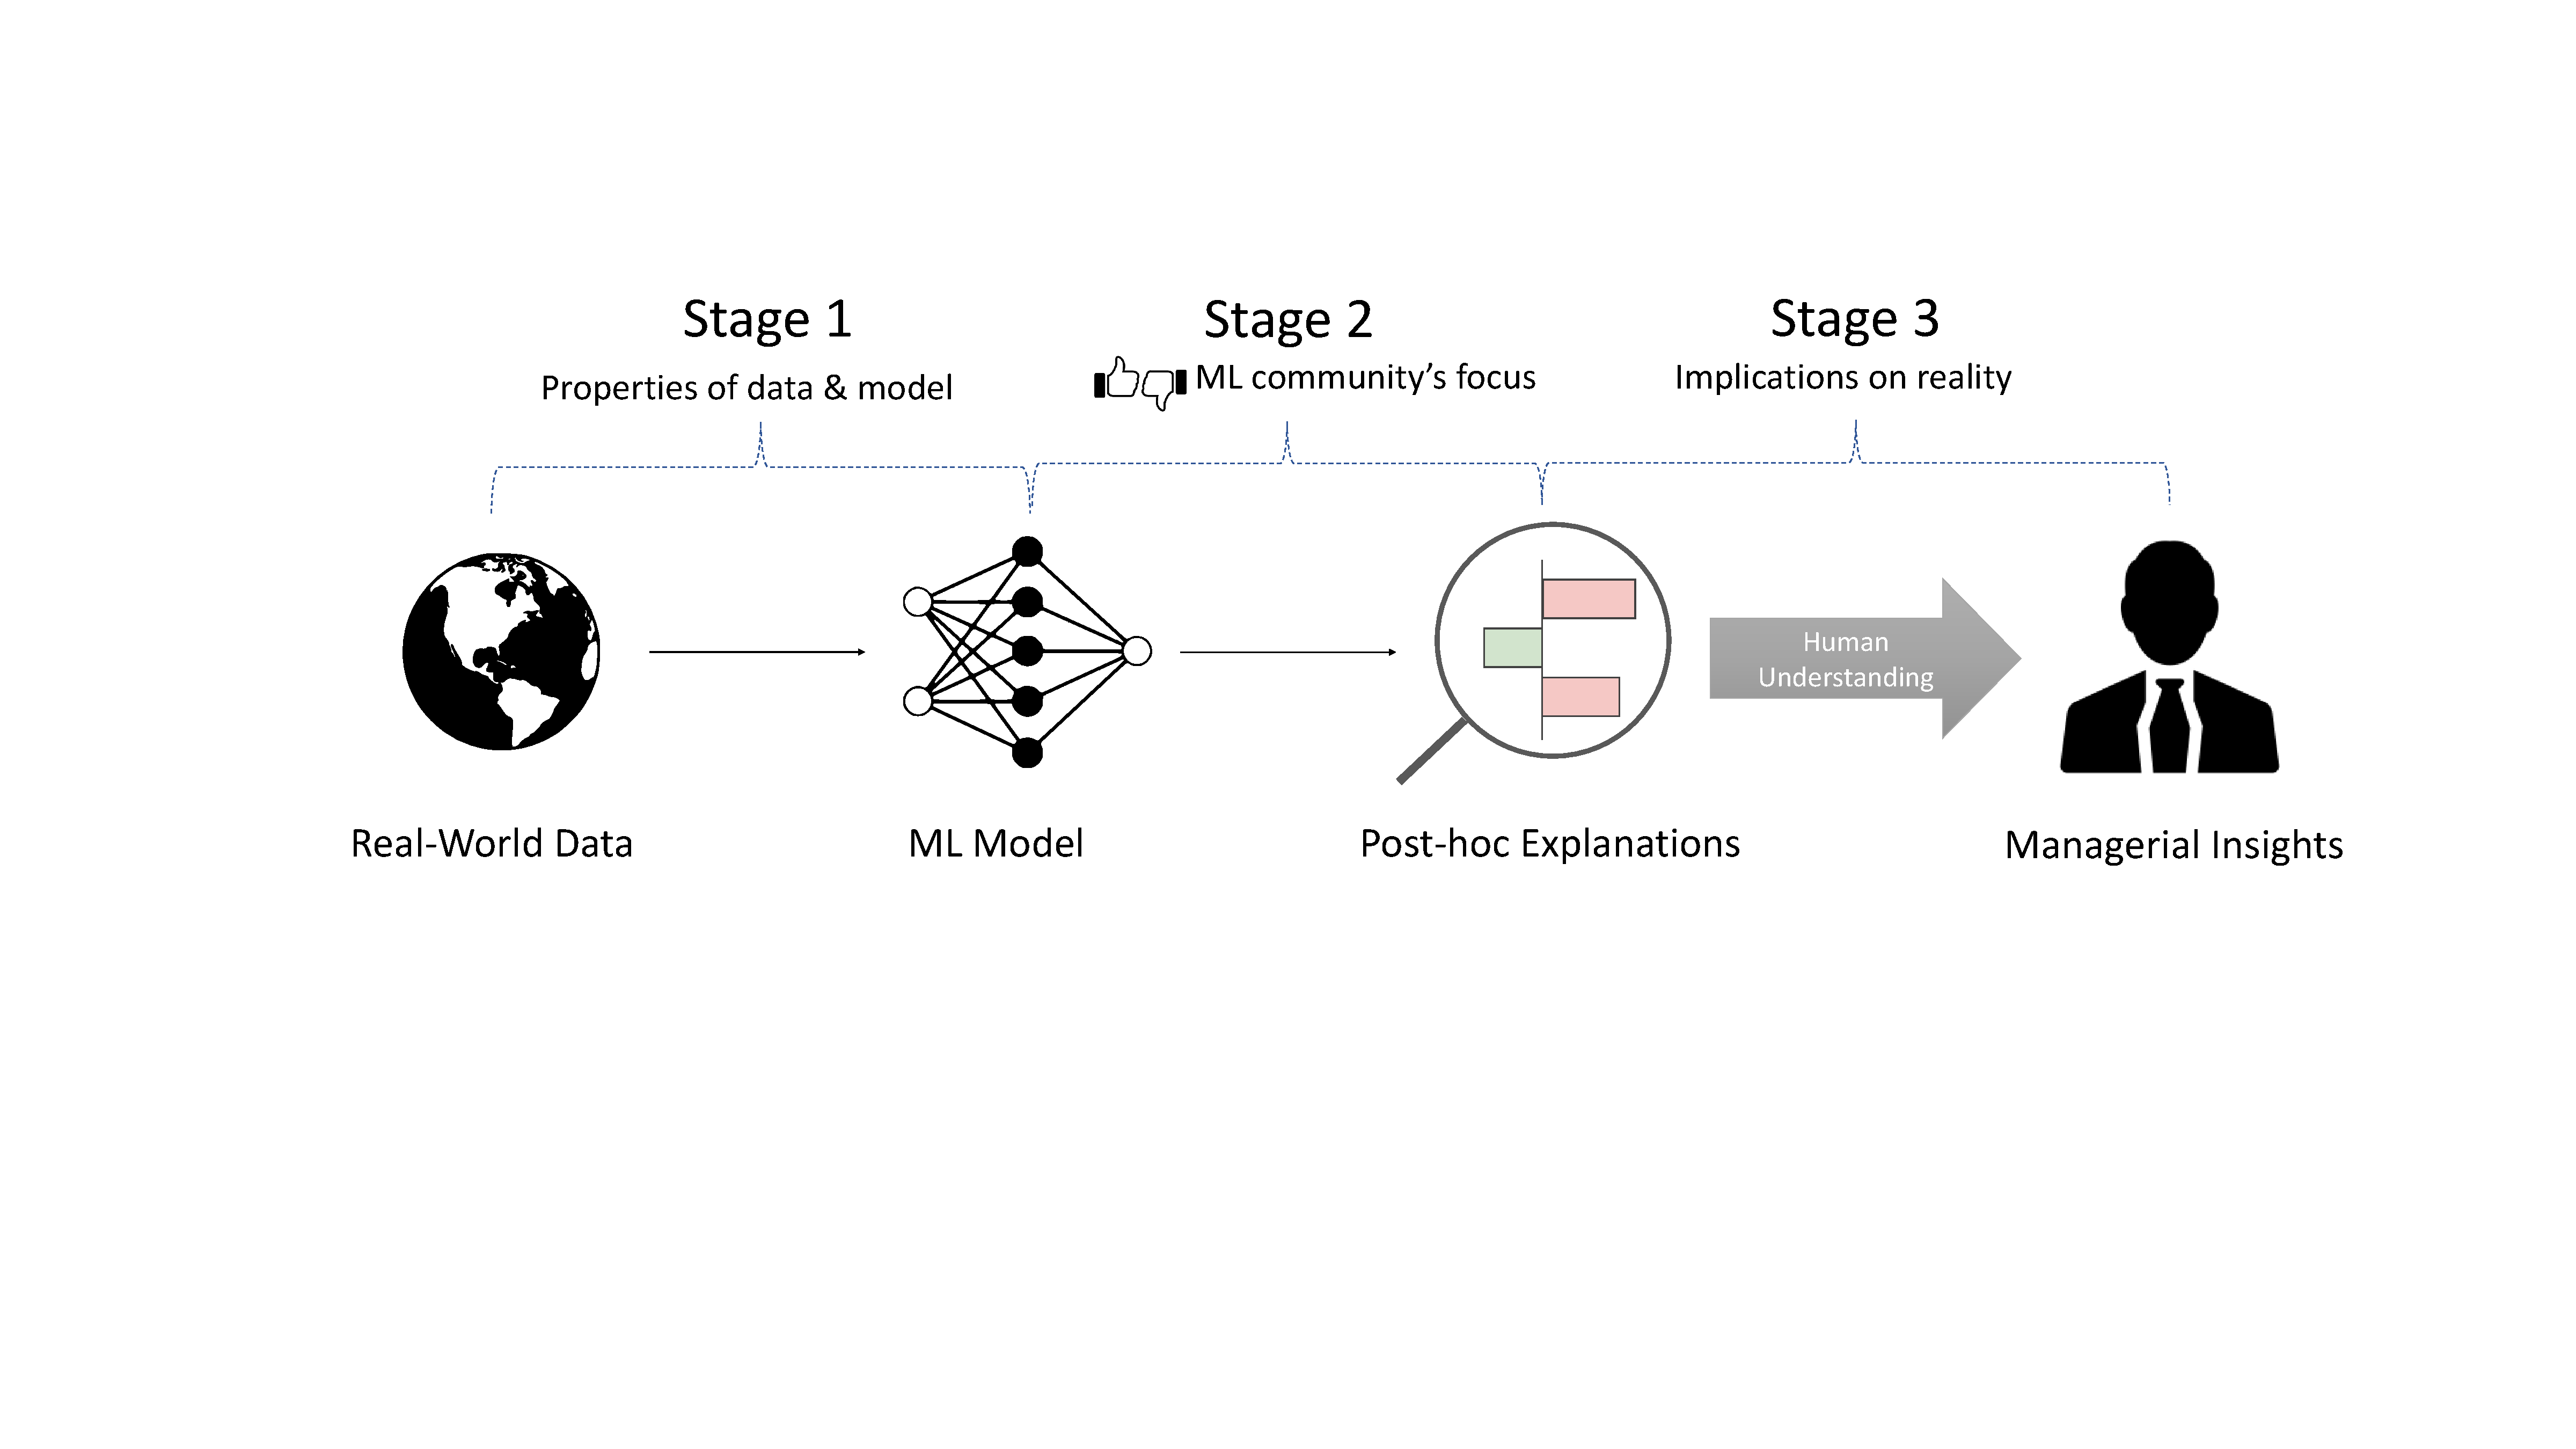
\includegraphics[width = \textwidth,trim=250 500 150 250 mm, clip=true]{Figures/pipeline.pdf}}
        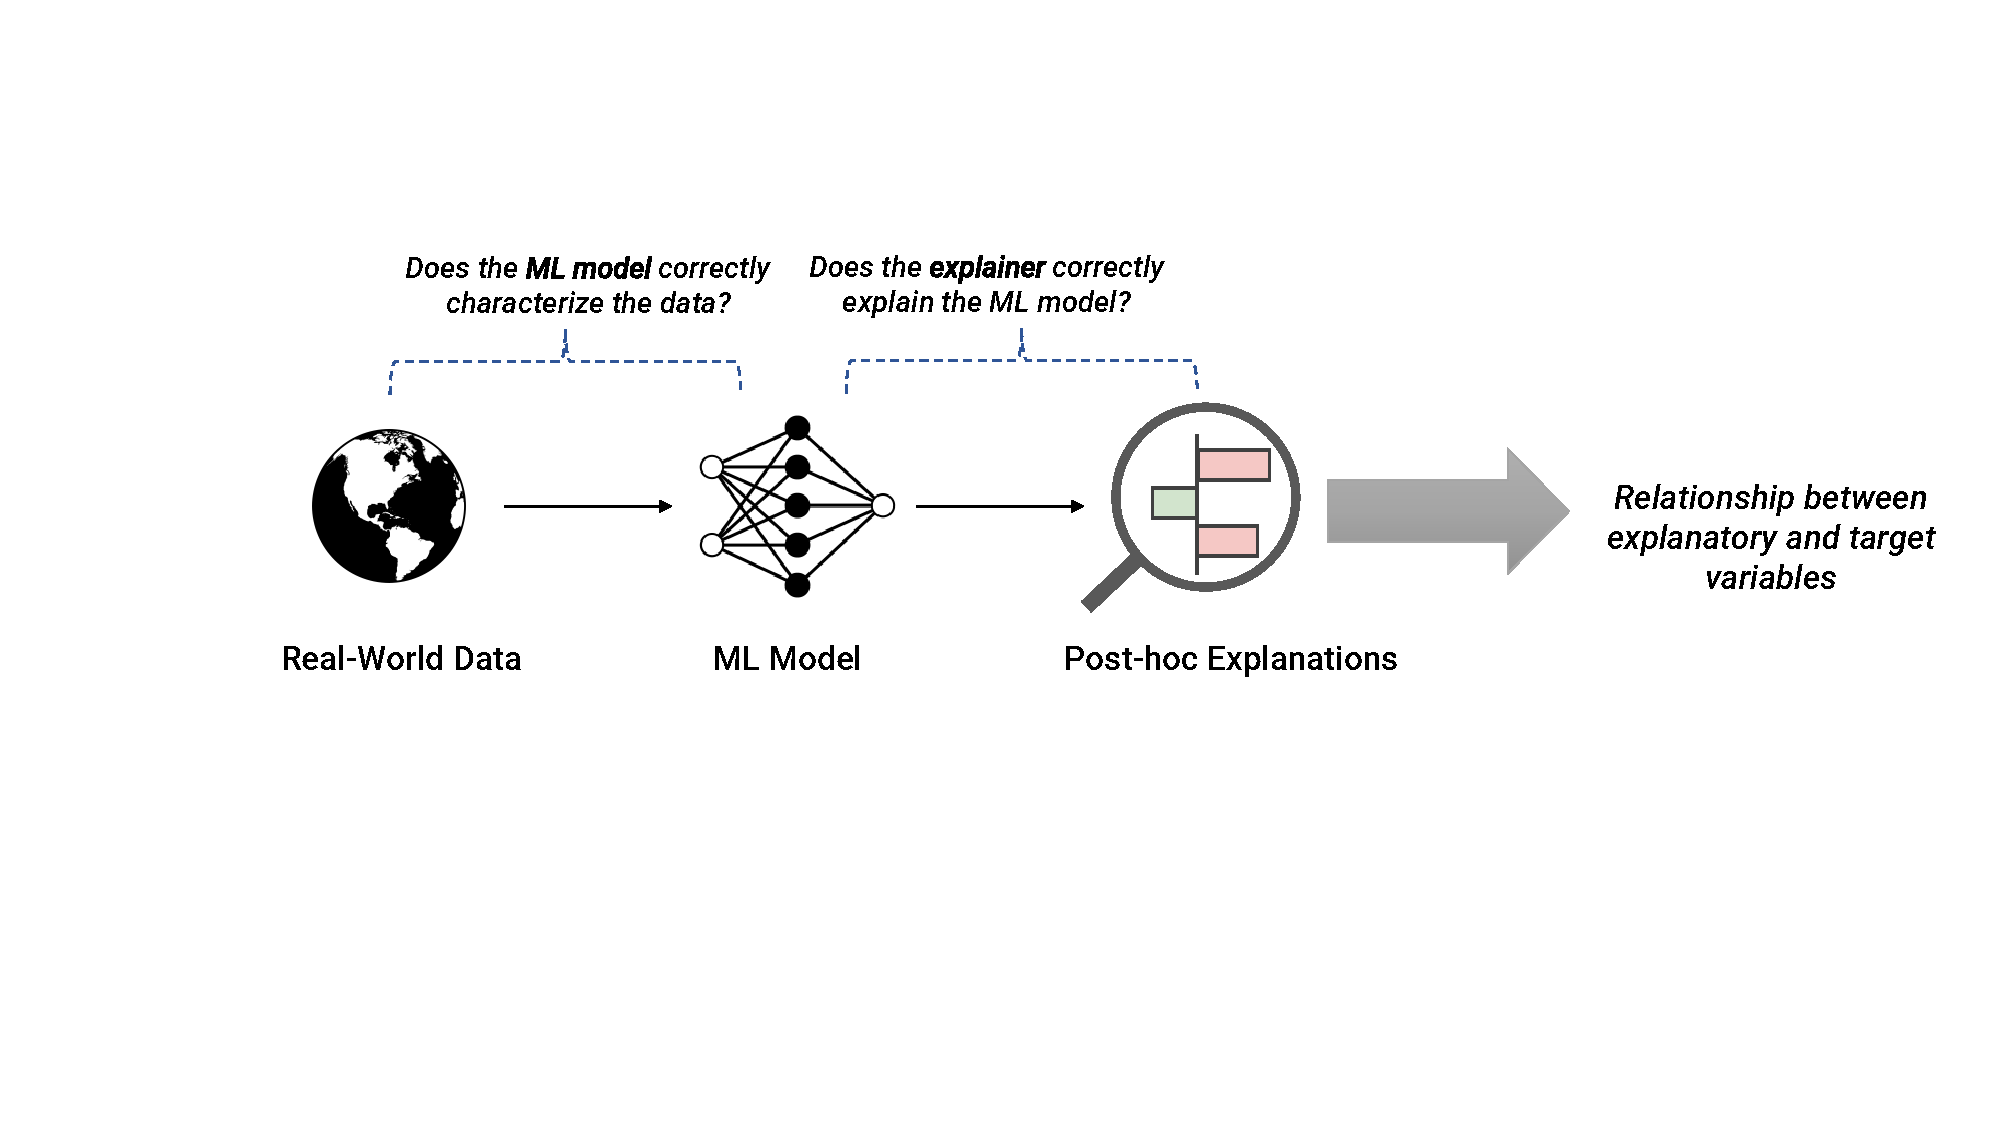
\includegraphics[trim={4.75cm 7.5cm 1.125cm 4.25cm},clip, width = 0.9\textwidth]{Figures/pipeline_flow_new.pdf}
        \caption{Explanation Pipeline: the pipeline of using post hoc explainers to explain a machine learning model. Additionally inferring information about the actual marginal effects of the features constitutes mistaken usage of the pipeline.}
        \label{fig:pipeline}
    \end{figure}
     % They build a black-box ML model for a complicated task, which could have many variables, or strong interactions of variables, or include unstructured data, such that canonical econometric methods do not easily apply. Then a post hoc explainer is used to generate feature importance for the ML model,  from which they draw some conclusions on the features as if they are using $\boldsymbol{\beta}$s. 
 

 
 % In addition, there are many types of feature importance \citep{AchenChristopherH1982Iaur}. However, except for \citep{lorentzen2020peeking}, the works cited in the previous paragraph did not provide a formal definition of feature importance and justify that the explainer(s) used were actually providing that type of feature importance. Similarly, the basic question of why Shapley values are appropriate feature importance measures is never addressed in these works\footnote{It is argued in \citep{kumar20shap} that Shapley values are not conducive to human understanding of feature importance.}. 


%Therefore, the goal of this paper is to urge the research community to approach post hoc explanations with skepticism and a more critical eye. 
% We argue in this paper that there exist fundamental flaws in using post hoc explanations to elicit information on $\boldsymbol{\beta}$s. 
Therefore, the goal of this paper is to conduct a thorough investigation into this new and emerging trend of research methodology so that we might advise the business research community
against this particular inappropriate use of post hoc explainers. We aim to directly answer the question, %``\emph{Can explanations from SHAP and LIME be extrapolated to infer $X$ and $Y$ relationship in the data?}''
``\emph{Can SHAP and LIME explanations capture the correct relationship between $X$ and $Y$, specifically the marginal effect of $X$ on $Y$, in the data?}''
with both empirical and theoretical evidence.  Specifically, we investigate whether the SHAP and LIME explanations align with marginal effects within three contexts that they are often used, as described previously. For this purpose, we design three metrics. The first evaluates whether an explanation's feature importance values have the same signs as the corresponding marginal effects. We call it the \textbf{directionality} of an explanation. The second metric evaluates how much the ranking of features by a post hoc explanation agrees with the ranking induced by the marginal effects. We call it the \textbf{concordance} of an explanation. The last metric evaluates whether a post hoc explanation identifies the most important features. We call it the \textbf{relevance} of the explanation. These metrics assess the extent to which the explanations are consistent with the marginal effects in terms of the sign, the ranking of features, and the identification of the most important features. We call the evaluation of the three metrics the test of \textbf{data-alignment}.

We evaluate the data-alignment of post hoc explanations using simulated data where we can control the ground truth marginal effects in the data. Our findings reveal that SHAP and LIME explanations typically do not align with marginal effects coefficients. This misalignment is evident even in straightforward business scenarios with a linear ground truth model. Such discrepancies remain notable even when the black box model being explained demonstrates high predictive performance on data containing all relevant features to $Y$, all of which are mutually independent. We then delve into the causes of this misalignment, discovering that various factors within the explanation pipeline affect explanation quality. These include having correlated features in the data, the predictive performance of the black box model, and specific settings of the explanation parameters. We corroborate the initial presentation of our results by showing that misalignment pervades an additional 100 simulations where we explain models produced using AutoML that were trained on datasets with varying numbers of features, rows, and label noise.


Critically, we offer a theoretical justification for why SHAP explanations inherently fail to align with the marginal effects, making Shapley values fundamentally inappropriate for any definite claims regarding marginal effects. We discuss in Section \ref{sec:theoretical_considerations} that SHAP estimates situational importance~\citep{StrumbeljErik2014Epma}, 
 which expresses the consequence of a feature taking on a value different from its mean. Although the computation of situational importance for a feature involves its marginal effect, the information it contributes can be destroyed in the process so that situational importance has no bearing on the marginal effect.%Moreover, we present theoretical grounds for conditions under which LIME might achieve a high degree of data-alignment.

% \textcolor{red}{I think we should say SHAP and LIME separately. }

% We then demonstrate another critical issue of post hoc explanations: inconsistency. Inconsistency refers to the difference in explanations produced by different configurations within the Explanation Pipeline. Using the same simulated data, we show that varying choices along this pipeline can lead to significantly divergent, and occasionally opposing, explanations. It then follows from the view that the purpose of science is to identify phenomena that occur without fail that post hoc explainers have very limited utility to researchers.


Finally, we explore potential strategies to increase the $\beta$-alignment of explanations provided by SHAP and LIME. Although our theoretical and empirical findings suggest that it is not possible to fully eliminate the issues of data-misalignment and inconsistency, they nevertheless reveal opportunities for improvement, which we address. For SHAP, the most immediate fix to increase data-alignment is to divide the Shapley values by the differences between the corresponding feature values and their means. For LIME, increasing some hyperparameters will significantly increase the alignment with the data.

Another strategy that showed promise involves averaging the explanations derived from a family of accurate models. We also observe that when the training data used by the black-box model include all relevant features, all of which are independent, the faithfulness of the explanations tends to increase. This suggests that the underlying data quality and structure play a significant role in the effectiveness of post hoc explanations.
However, other intuitive strategies we tested, such as combining explanations from both SHAP and LIME for a single black-box model or increasing the local approximation accuracy of LIME, did not yield effective results. This highlights the complexity of the issue and the need for more nuanced solutions.
It is also important to note that while our proposed mitigation strategies improve data-alignment to various degrees, they do not completely resolve the issues of misalignment and inconsistency inherent in SHAP and LIME. Consequently, post hoc explainers such as SHAP and LIME should be used with great caution and for the correct purpose by business researchers. %Specifically, researchers should not rely on post hoc explanations to validate hypotheses in data. %add something about robustness/causal forest here??????

    
 

   % Our main contributions can be grouped into the following two parts. First, we give a novel systemization of the use of post hoc explainers that illuminates how and why post hoc explainers may not give business researchers correct understanding of $\boldsymbol{\beta}$, as well as what kinds of errors the explanations can contain and how the errors could negatively affect businesses and researchers. Our proposed system addresses vulnerabilities in the pipeline shown in Figure \ref{fig:pipeline} that business researchers are encouraged to keep in mind or mitigate in order to successfully glean managerial insights from post hoc explainers. We develop the system over the course of the paper by first demonstrating the issues, then identifying the causes of the issues. The second main component of our contributions is a set of mitigation strategies for misalignment and inconsistency that we propose and test. 
   
%This research paper presents significant contributions to the understanding and application of explainable AI in business research, focusing on two or three key areas.

% Firstly, a key contribution is the critical examination of the emerging use of a popular yet not rigorously validated methodology in business research: using SHAP and LIME to infer $\boldsymbol{\beta}$. The paper provides a nuanced critique, showing that these widely used tools often fail to convey accurate information about $\boldsymbol{\beta}$.  This critique is substantiated with empirical evidence using a simulated dataset, which demonstrates the misalignment of these explanations even under ideal conditions.  This finding is crucial as it challenges the prevailing trend in business research that heavily relies on these tools for understanding the dynamics of $\boldsymbol{\beta}$.

% Secondly, the paper contributes by exploring the reasons behind the misalignment and inconsistency of post hoc explanations. It delves into both theoretical and empirical aspects, revealing how various factors, including model hyperparameters and the underlying data structure, influence the quality of these explanations. This analysis not only adds depth to our understanding of the limitations of post hoc explainers but also highlights the complexity involved in extracting meaningful insights from machine learning models in business contexts.

% Lastly, the paper proposes potential strategies to improve the quality of explanations from post hoc explainers. One notable strategy is averaging explanations across a family of accurate models, which shows promise in mitigating some of the identified limitations. While acknowledging that these strategies do not fully resolve the issues of misalignment and inconsistency, the paper provides a constructive directionality for future research and application, emphasizing the need for caution and informed decision-making when using post hoc explainers in business research.

% Note that our work is fundamentally different from critiques on post hoc explanations in the machine learning community.

Overall, our paper identifies and cautions against a growing trend of the inappropriate use of post hoc explanations to draw definite conclusions on data. We argue that post hoc explanations should not be used to \textbf{validate} hypotheses about data; instead, their role in gathering knowledge about data should be limited to \textbf{proposal} of hypotheses. To gain an accurate understanding of the underlying relationships between $X$ and $Y$ in the data, we emphasize the need for more rigorous and comprehensive follow-up analyzes, both quantitatively and qualitatively. This distinction is essential to ensure the prevention of the overestimation of the reliability and validity of insights derived from machine learning models in business research.

% Our system addresses the following questions which are of particular interest to the business community, and therefore not investigated in prior machine learning works on post hoc explainer efficacy. 
% \begin{enumerate}
%     \item How well can post hoc explanations faithfully explain a simple linear ground truth underlying a black box model's training data?
%     \item Will explanations obtained from different configurations of the pipeline contain an internally consistent narrative, such that I do not need to worry too much about my choice of data pre-processing, black box, explainer, and explainer settings? 
%     \item What strategies can I adopt to increase the likelihood that the managerial insights I glean from post hoc explanations are actually valid in reality?
%     %\item What steps can I take to address choice paralysis induced by the many possible configurations of the pipeline?
% \end{enumerate}

    The paper is organized as follows. We will review related work in Section \ref{sec:related_work}. Then we use a simulated dataset with ground-truth models that we create to demonstrate the Explanation Pipeline and its vulnerabilities in Section 3.  We provide theoretical and empirical analyses on why post hoc explanations are not suitable to infer information about marginal effects in Section 4. Section 5 discusses another limitation of post hoc explanations, the inconsistency, which further hinders its use in practice. We then showcase some mitigation strategies for SHAP and LIME in Section \ref{sec:mitigation_strategies} and subsequently gauge how beneficial they are over baselines in reproducing the findings of an econometric study carried out using real loan application data in Section \ref{sec:case_study}. The paper concludes in Section \ref{sec:discussion} with a summary of our findings and final remarks on post hoc explanations and their use in business research. In the appendix, we corroborate all of the experiments in the main body of the paper by running them a second time using a synthetic direct marketing dataset. 
    
\section{Related Work}
    \label{sec:related_work}
    This section introduces SHAP and LIME and then reviews the prior literature that discusses their weaknesses. %Weaknesses discussed include intrinsic (theoretical) issues due to how the explainers are designed, and practical issues users may face due to those intrinsic issues. 

    \subsection{Post Hoc Explainers - SHAP and LIME}
     SHAP \citep{lundberg17shap} and LIME \citep{ribeiro16lime}  are the two most widely used post hoc explainers. %Model agnosticism refers to the ability to explain any ML model without the access to the internals of the ML model, i.e., only using the input and output of a model. Attributive explainers explain the predictions of a predictive ML model by attributing numerical feature importance values to each input feature. Both SHAP and LIME represent feature importance using the coefficients of an additive feature importance model. %Counterfactual explainers such as WachterCF\citep{wachter17wachtercf} and DiCE\citep{mothilal20dice} are of secondary importance and explain an output of an ML model by providing a contrasting input that cause the model to produce a different output. 
        We use SHAP and LIME as representatives for post hoc explainers in this paper because they constitute the dominant use case for post hoc explainers in business research.

        % Counterfactual explainers explain an output of an ML model by providing a contrasting input that cause the model to produce a different output. It is desirable for the contrasting input to be as close to the original as possible in order to identify a minimal change that yields a different output. Examples of counterfactual explainers include WachterCF\citep{wachter17wachtercf} and DiCE\citep{mothilal20dice}.
        
     %SHAP and LIME are model-agnostic attributive post hoc explainers. They are model-agnostic in the sense that they can explain any ML model.  Standard implementations of SHAP and LIME can explain both classification and regression models using tabular, text, or image data as input.

\paragraph{SHAP}
SHAP (SHapley Additive exPlanations) is a groundbreaking approach in the field of interpretable machine learning that offers a unified measure of feature importance. Developed by Lundberg and Lee in 2017, it builds on the concepts of game theory, particularly the Shapley value, to assign an importance value to each feature for a particular prediction. The fundamental idea behind SHAP is to assess the contribution of each feature to the difference between the actual prediction and the average prediction over the dataset. One of the unique aspects of SHAP is its consistency and local accuracy. The method guarantees that if a model changes in a way that makes a feature more important, the SHAP value of that feature will not decrease. Local accuracy ensures that the contributions of all features sum up to the actual prediction minus the average prediction, providing a detailed and accurate decomposition of the prediction. Note that LIME does not have this local accuracy property. There are several variants of SHAP, such as Kernel SHAP \citep{lundberg17shap}, TreeSHAP \citep{lundberg2018consistent} and DeepSHAP \citep{lundberg17shap}. Each variant retains the core principles of SHAP while adjusting the computational strategy to suit the specific model architecture, ensuring that the interpretability benefits of SHAP can be realized across a wide range of machine learning models.
    % SHAP's additive feature importance model differs from LIME's in that the coefficient of each feature represent the Shapley value~\citep{shapley97shapley} of that feature. SHAP surrogate models are not fit on sampled training data instances directly like LIME's, but rather on sampled coalition vectors (binary vectors indicating presence of each feature). Shapley values were originally a game-theoretic notion meant to quantify how much each player contributed to the final score of a game. In the context of SHAP, the Shapley values (surrogate model coefficients) represent how much the value of the feature to which they correspond contributes to the final value of the black-box model's prediction. 

    
\paragraph{LIME}  % Underlying LIME explanations are ridge regressors fitted on data sampled around the input datum being explained. 
LIME is the very first model-agnostic post hoc explainer developed by \citet{ribeiro16lime}. In the (default) implementation of LIME by its authors, the input data are discretized and LIME trains a ridge regressor on a synthetic dataset constructed by sampling uniformly around the input datum. The coefficients of the ridge regressors indicate the importance of each feature. LIME discretizes numerical features into quartiles to avoid dealing with problems associated with differing scales of features and ensure users do not get confused when interpreting negative weights for negative valued features. The ridge regression's optimization weighs the sampled data with an exponential kernel and includes an $L_1$ (LASSO) penalty to encourage explanations to be sparse. The ridge regressors are called surrogate models because they are trained to approximate the predictions of the black box model.
    
    LIME's ridge coefficients are meant to represent marginal effects, but depending on the LIME variant and the model being explained, are not the gradient of the black box model at the input being explained. \citet{garreau20theoretical,garreau2020looking} proved that the original LIME formulation's coefficients did not, in general, equal the gradient of the black box model at the input being explained. Instead, each feature importance value is proportional to the partial derivative of the black box at the input datum and the proportionality constants differ by feature. \citet{agarwal21clime} showed that a simpler variant of LIME called C-LIME that does not discretize input features and does not perform weighted ridge regression produced coefficients that are proportional to the gradient of the black box model. %Removing discretization allows C-LIME to recover the gradient because otherwise, local information about the black box's decision boundary is destroyed.
    In discretizing features, the data used in LIME's regression problem consists of binary features indicating which bins (quantiles) the feature values of sampled data fall into, which destroys the gradient since the local information about the black box's decision boundary is lost. Moreover, C-LIME drops the ridge penalty because enforcing sparsity opposes the goal of recovering the gradient. In the specific case where the model being explained is linear, C-LIME recovers the coefficients of the linear model. Thus in this paper, we choose to disable the discretization setting of LIME throughout the paper.



    \subsection{The Faithfulness and Interpretability of Post hoc Explanations}
        \label{sec:cs_critique}
        The alarm for post hoc explanations had first gone off in the field of machine learning, as researchers questioned the correctness and validity of post hoc explanations. However, the notions of correctness and validity in the ML literature differ from the point of view we take in this paper. The machine learning community's attention has mainly focused on explanation quality \textbf{with respect to the ML model} since the primary goal of the machine learning field is to develop new models that make better or faster predictions. In addition, they consider factors relating the ability of humans to interpret the explanations, most of which do not fall within the scope of our critique. Thus, the way the ML community evaluates explainers is different from how we will evaluate them in this paper.

    
        That post hoc explainers misrepresent the black boxes they explain is a pillar of the ML community's critique. The terms \emph{fidelity} and \emph{faithfulness} are used interchangeably and generally represent the maxims of completeness and soundness outlined by \citep{zhou21evaluating}. An explanation is complete if it is a full characterization of the black box's behavior. An explanation is sound if its characterization is correct.\footnote{In this paper, however, we characterize faithfulness in reference to the ground truth instead of the black box model because we are interested in obtaining insights about reality, not about black box models. In Section \ref{sec:evaluating_faithfulness}, we define metrics that capture our notion of faithfulness.} 
    \cite{garreau2020looking} and \cite{han22which} consider soundness from a function approximation perspective, directly measuring the difference between an explainers underlying model and the black box function. \cite{garreau2020looking} shows that LIME's approximation error is always bounded away from 0. \cite{han22which} analyzes kernelSHAP and LIME relying on a view of KernelSHAP and LIME as kernel weighted linear regression models whose input data are sampled by perturbing the input to be explained by a noise random variable. They remark that the choice of noise distribution made by kernelSHAP and LIME prevents them from being able to recover the gradient of linear models they explain as feature importance values. It follows that KernelSHAP and LIME cannot necessarily be expected to reliably perform their intended task of interpreting black box model behaviors. 
%We will show in this paper how the different design choices in the modeling process will cause inconsistency of post hoc explanations and make resulting inferences about $\boldsymbol{\beta}$ unreliable. 
Other fidelity/faithfulness metrics measure particular approximation properties such as the extent to which an explainer assigns zero importance to features the model does not depend on are used as metrics in \cite{nguyen2020quantitative}. Metrics such as Deletion and Insertion metrics are based on the idea that features said to be important by an explainer should have significant effects on black box output \citep{deyoung20eraser,nguyen2020quantitative,alvarez18robustness,luss2021leveraging}.
%The underlying supposition of Deletion and Insertion metrics is that removing or adding features said to be important to a prediction by an explainer should change the prediction to change substantially \citep{deyoung20eraser,nguyen2020quantitative,alvarez18robustness,luss2021leveraging}. %Some works evaluate explainers by taking advantage of contexts where feature importance information of a model is known. \cite{blunsom2019can} evaluates explainers of a white box recurrent model by quantifying the explainers' error rates with respect to identifying important tokens in inputs. \cite{carmichael21framework} evaluates additive explainers by calculating the Jaccard index between the sets of effects present in neural networks and GAMs and the effects and associated contributions of features given by explainers for those models. 
    
  The machine learning community has also largely focused on other aspects of post hoc explanations, such as interpretability or understandability of the explanations.   Explainers which satisfy desiderata related to  interpretability should be able to provide a description of the behavior of a black box model in a form which can be easily understood by humans. For example, explanations should be simple enough to be intelligible but complex enough so that the explanation is still complete and sound. Parsimony \citep{nguyen2020quantitative} and clarity \citep{lakkaraju2017interpretable,montavon2018methods,alvarez18robustness} metrics, for example, measure the simplicity and ambiguity of explanations, respectively\footnote{We use the terminology of \cite{markus2021role} here.}. \cite{jacovi2023diagnosing} further requires that the form of explanations match what the psychology literature identifies as natural for human understanding.  Simplicity of explanations beyond the per-feature importance values given by attributive explainers is not desirable in our application because, e.g. artificial enforcement of sparsity could encourage explanations to omit information about the marginal effects and become incomplete and unsound as a result. For example, LIME's use of a LASSO penalty to make its explanations sparse is undesirable because it could cause a feature to have zero importance when the $\beta_j$ for that feature is non-zero. %Futhermore, stability metrics quantify how different explanations of nearby inputs are. The size of the local Lipschitz constant of the function underlying the explainer is one such example \citep{alvarez18robustness}. Stable explanations can be desirable because an explainer's explanations for two similar inputs being very dissimilar could engender mistrust of the explainer or arouse unwarranted suspicion of unfairness in the underlying decision process. These factors, however, are not within the scope of our discussion.

    
   
    \section{Use of SHAP and LIME in Business Research}
% \textcolor{red}{find papers that use post hoc explanation to get insights that resemble $\boldsymbol{\beta}$ (explaining G). Also mention that some papers only use post hoc explainer on M. It is the intended use of the post hoc explanations, but even that faces severe criticism from the ML community discusses explanations for M}

% \textcolor{red}{Move the appendix here}
        As part of our literature review process, we cataloged papers at the intersection of business and explainable machine learning. We used Web of Science to search for publications citing at least one of LIME~\citep{ribeiro16lime} or SHAP~\citep{lundberg17shap} and have either ``LIME" or ``SHAP" appear in the body of the paper.  The results were filtered by topics related to business, such as management, economics, supply chain \& logistics, operations research \& management science, etc. 
        We then iterated through hundreds of resulting papers one by one, collecting papers that actually used SHAP or LIME to explain a machine learning model (some papers only mentioned SHAP or LIME in the contexts of related work or future work) until we had a total of 150 papers. Out of these papers, \textcolor{red}{97\% used SHAP and 8.6\% used LIME to generate explanations for their models, including 6\% using both of them.} \textcolor{blue}{Ronilo, the maths still do not add up. 97 + 8.6 - 6 = 99.6, not 100}

        
        We took a close look at these papers and characterized the papers' use of post hoc explanations by following three steps. We first searched for evidence that it was understood that the intended use of SHAP and LIME is to explain model outputs (rather than the data). Then, we searched for four forms of problematic language indicative of inappropriate use of post hoc explanations and recorded quotations of each type (if available). Appendix Table \ref{tab:mistakes} provides examples of each language form. Not all papers contained such language; in some papers it was clear or made explicit that they used SHAP and LIME only within the scope of model explanation. Having identified any quotations which we deemed problematic, we then divided the papers into three categories: papers that clearly extrapolated explanations to glean information about the marginal effects, papers whose wording could suggest extrapolation, and papers that only used explanations for model interpretation.% Note again, though, that both SHAP and LIME fall short for their indented purpose and face intense scrutiny from the ML community \cite{kumar20shap,garreau2020looking}.

%\textcolor{red}{add a summary of the findings \&statistics from the 116 papers}
%\textcolor{red}{double check and update the numbers}
        We found that 42\% of the papers clearly extrapolated explanations to gain insight into the marginal effects in the data. In addition to that, there is another \textcolor{red}{21\%} that at least used unclear language such that readers could interpret their findings as being made about the marginal effects. This means that more than half of the papers we sampled had some problematic language. Further, \textcolor{red}{76\%} of the papers which had clear over-extrapolation were from top journals\footnote{A journal was considered a ``top journal" if it is an INFORMS journal or its most recent 5-year impact factor according to Clarivate's Journal Citation Reports (JCR) was at least 5.0 at the time of writing (April 2024).}.
        %Given the popularity of SHAP and the idea that the presence of this problem in publications from top journal is indicative of the pervasiveness of the problem, we also separately surveyed papers from the INFORMS family of journals that used SHAP to explain a machine learning model. About 25\% of these papers had clear extrapolations, and 17\% could be construed as having extrapolated. Thus it was still the case that about half of the papers using SHAP contained problematic language.
        Consequently, we estimate that a substantial portion of business literature that use SHAP or LIME to explain a machine learning model make inappropriate use of their feature importance values to gain insight into the marginal effects.

        The interpretation of SHAP and LIME feature importance in each paper fell into three categories: 1) identifying the directionality of impact of each feature (i.e., feature importance sign), 2) ranking features by relative importance, and 3) identifying a subset of the most important features. Table \ref{tab:metric_examples} below records prototypical ways in which authors expressed their desire to perform these tasks. In Section \ref{sec:evaluating_faithfulness}, we define metrics to characterize the ability of an explainer to perform these tasks. We call them directionality, concordance, and relevance, respectively. 

        
% \begin{table}[htbp] 
%     \tiny
%     \caption{Correspondence Between Paper Language and Our Metrics}
%     \begin{tabu} to 1\linewidth { | X[l] | X[l] | X[l] | X[l] |}% X[l] | X[l] |}
%        \hline
%        \textbf{Purpose} & \textbf{Example 1} & \textbf{Example 2} & \textbf{Example 3}\\
%        \hline
%        \textbf{Identifying How Features Impact on the Target (Direction)} 
%        & Positive SHAP values indicate that the variable has a facilitative effect on bike-sharing use, while negative values indicate a suppressive effect
%        & If there are more blue dots with negative SHAP values and more red dots with positive SHAP values, the values of that feature would be positively correlated with the prediction
% results. In other words, customers with higher scores for this characteristic are more likely to be churners. 
%        & For example, the spec values with positive mean SHAP are recommended options in product design because they have positive effects on customers’ choices. \\ \hline 
%        \textbf{Ranking the Features by Relative Importance (Concordance)}
%        &This study contributes fourfold to the literature, and findings provide several insights for station-area last-mile facility planning. First, it explicitly assesses the relative importance and associated rankings of last-mile facilities, the built environment and metro network attributes in predicting metro ridership
%        & We find that the application of Shapley values enables us to assess both the identification and the ranking of relevant explanatory variables for the investigated target variable. 
%        &  Using SHAP, we show the ranking of importance of features and visualise the exact impact patterns of the most important features on the target variable. This transparency provides policy makers with credible quantitative evidence that enables a targeted approach to improving road schemes and management, ultimately leading to a reduction in serious traffic accidents.  \\ \hline
%        \textbf{Identifying the Top-$k$ Features (Relevance)}
%        & These three CV factors ranked at the top three in terms of the relative importance of SHAP values. Their SHAP values also raise with the increase of corresponding CV values, revealing that alternative routes with large difference in travel distances, travel speeds or signalized intersection numbers would lead to higher degrees of disequilibrium states at the road network.
%        & the Shapley Additive Explanations (SHAP) method is integrated with the XGBoost classifier to identify the key risk-contributing traffic features.
%        & By implementing XAI to identify the most critical indicators/factors that contribute to harmful emissions, a controlled and measured approach can be taken to monitor the fluctuations of these indicators over time. \\ \hline
%        \textbf{Other Usage}
%        & (\textbf{OLS Alternative}) Hence, the applied black box algorithm in combination with Shapley values allows to unbox the black box ML approach and provides similar economic insights as provided by pooled OLS 
%        & (\textbf{Theory Confirmation}) XGBoost, is utilized to capture the quantitative associations, and the SHAP (Shapley Addictive exPlanation) model is used to interpret the results from XGBoost. Our results provide empirical support for prior theoretical findings based on mathematical equilibrium models  
%        & (\textbf{Recourse Advocacy}) Since the number of bus stops, bus lines, bike-sharing trips, parking lots and pedestrian shed ratio have high SHAP importance and substantial effects on metro ridership, relevant last-mile transport facilities should be given sufficient attention by transport planners and operators to enhance these access modes to metro stations. \\ \hline
%    \end{tabu}
%    \label{tab:metric_examples}
%    \end{table}

% ANONYMIZED VERSION

\tw{Please fix Table 1. The spacing between items in the examples are not consistent. }
\begin{table}[htbp]
\small
\caption{Correspondence Between Paper Language and Our Metrics.  Statements appearing in angle braces $\langle \cdot \rangle$ 
are meant to make the statements more general. The $X_j$ represent data features and $Y$ represents the outcome of interest.}
\begin{tabu} to 1\linewidth {  P{3cm} | X[l]  }
\toprule
\textbf{Purpose} & \textbf{Examples} \\
\hline
\textbf{Identifying How Features Impact the Target (Directionality)}
& ``...Positive SHAP values indicate that the variable has a facilitative effect on $\langle Y\rangle$, while negative values indicate a suppressive effect..." \\ 
& \vspace{-.8cm}``...Individuals whose predictions received larger SHAP values for this feature are more likely to have $\langle Y=1\rangle$..."\\
& ``...Choosing features with positive mean SHAP are recommended options because they have positive effects on $\langle Y\rangle$..." \\
\hline
\textbf{Ranking the Features by Relative Importance (Concordance)}
& ``...This study provides insights for planning the design of $\langle X\rangle$ by assessing the relative importance and associated rankings of the $\langle X_j\rangle$ in predicting $\langle Y\rangle$..."\\\smallskip
& \vspace{-.8cm}``...The use of Shapley values enables us to identify and rank relevant $\langle X_j\rangle$ for the investigated $\langle Y\rangle$.."\\\smallskip
& ``...Our feature rankings and visualizations of impact patterns provide policy makers with evidence for strategies to improve $\langle Y\rangle$..." \\
\hline
\textbf{Identifying the Most Important (Top-$k$) Features (Relevance)\hspace{3cm}}
& ``...That $\langle X_1$, $X_2$, and $X_3\rangle$ have the top-3 SHAP values and that their SHAP values are positive reveals that increasing $\langle X_1$, $X_2$, and $X_3\rangle$ would lead to larger $\langle Y\rangle$..."\\\smallskip
& \vspace{-.8cm}``...We use SHAP explanations of an XGBoost Classifier to identify the key features which contributing to the risk $\langle Y\rangle$..."\\\smallskip
& ``...By using XAI to identify the most important factors and indicators that contribute to $\langle Y\rangle$, their values and fluctuations can then be monitored over time..." \\
\hline
\textbf{Other Usage}
& (\textbf{OLS Alternative}) ``...The combination of a black box algorithm and SHAP provides similar economic insights as provided by pooled OLS..."\\\smallskip
& (\textbf{Theory Confirmation}) ``...SHAP is used to interpret the quantitative associations found by XGBoost; our results provide empirical support for prior theoretical findings..."\\\smallskip
& (\textbf{Recourse Advocacy}) ``...Since $\langle X_1$, $X_2$, and $X_3\rangle$ have high SHAP importance and substantial effects on $\langle Y\rangle$, $\langle X_1$, $X_2$, and $X_3\rangle$ should be given attention by policy makers to increase $\langle X_1$, $X_2$, and $X_3\rangle$..." \\
\bottomrule
\end{tabu}
\label{tab:metric_examples}
\end{table}
% \begin{table}[htbp] 
%     \tiny
%     \caption{Correspondence Between Paper Language and Our Metrics. The $X_j$ represent data features and $Y$ represents the outcome of interest.}
%     \begin{tabu} to 1\linewidth { | X[l] | X[l] | X[l] | X[l] |}% X[l] | X[l] |}
%        \hline
%        \textbf{Purpose} & \textbf{Example 1} & \textbf{Example 2} & \textbf{Example 3}\\
%        \hline
%        \textbf{Identifying How Features Impact on the Target (Directionality)} 
%        & Positive SHAP values indicate that the variable has a facilitative effect on $Y$, while negative values indicate a suppressive effect
%        & Individuals whose predictions received larger SHAP values for this feature are more likely to have $Y=1$. 
%        & Choosing features with positive mean SHAP are recommended options they have positive effects on $Y$. \\ \hline 
%        \textbf{Ranking the Features by Relative Importance (Concordance)}
%        & This study provides insights for planning the design of $X$ by assesses the relative importance and associated rankings of the $X_j$ in predicting $Y$
%        & The use of Shapley values enables us to identify and rank relevant $X_j$ for the investigated $Y$. 
%        & Our feature rankings and visualizations of impact patterns provide policy makers with evidence for strategies to improve $Y$ \\ \hline
%        \textbf{Identifying the Top-$k$ Features (Relevance)}
%        & That $X_1$, $X_2$, and $X_3$ have the top-3 SHAP values and that their SHAP values are positive reveals that increasing $X_1$, $X_2$, and $X_3$ would lead to larger $Y$.
%        & We use SHAP explanations of an XGBoost Classifier to identify the key features which contributing to the risk $Y$.
%        & By using XAI to identify the most important factors and indicators that contribute to $Y$, their values and fluctuations can then be monitored over time. \\ \hline
%        \textbf{Other Usage}
%        & (\textbf{OLS Alternative}) The combination of a black box algorithm and SHAP provides similar economic insights as provided by pooled OLS 
%        & (\textbf{Theory Confirmation}) SHAP is used to interpret the quantitative associations found by XGBoost; our results provide empirical support for prior theoretical findings..
%        & (\textbf{Recourse Advocacy}) Since $X_1$, $X_2$, and $X_3$ have high SHAP importance and substantial effects on $Y$, $X_1$, $X_2$, and $X_3$ should be given attention by policy makers to increase $X_1$, $X_2$, and $X_3$. \\ \hline
%    \end{tabu}
%    \label{tab:metric_examples}
%    \end{table}

\section{Explanation Pipeline}
    \label{sec:pipeline_demo}
    In this section we will use a simulated dataset to demonstrate the explanation pipeline many papers follow to elicit information about features.
    
An explanation pipeline consists of two stages. First, a machine learning model, denoted by $\mathcal{M}$, is trained on data $\mathcal{D}$. We call this stage the \emph{prediction stage}. Then, an explainer model (e.g., LIME or SHAP), denoted by $\mathcal{E}$, is applied to $\mathcal{M}$ to generate explanations. We use $e_{\mE}(x^{(i)}_j)$ to represent an explanation (e.g., feature importance) regarding feature $X_j$ of $\mE$'s prediction for the $i^{\text{th}}$ data instance $\mathbf{x}^{(i)}$. We call this second stage the \emph{explanation stage}. % We will also use the notation $\mathbf{x}^{(i)}$ to represent test set instance $i$. % building a machine learning
    
    We illustrate the Explanation Pipeline with a simulated loan approval dataset\footnote{Real datasets are not suitable for the experiments in this paper because we require access to the ground truth in order to evaluate the faithfulness of the post hoc explanations. However, in Section \ref{sec:case_study}, we will conduct a case study using a real loan application dataset and use the results of a published econometric study using that dataset as the ground truth}. Our simulated dataset models the task of predicting whether an individual will be approved for a loan based on their demographic features and credit-related features. We define the model for generating the dependent variable so that the ground truth is known and controllable. We also define the ground truth model to be linear, such that the explanation task is relatively easier for the post hoc explainers. %Some of the features are not independent. We demonstrate in Section \ref{sec:role_of_correlation} that the lack of feature independence effects data-alignment. This being the case, we test our mitigation strategies in Section \ref{sec:mitigation_strategies} using a variant of the data generation process where all features are mutually independent in order to control for the effect of feature correlation and focus on the effect of our mitigations.                                       
    In the following, we will describe how we generate our data and then apply the pipeline to a sample dataset using SHAP. This data and its variant will be used throughout the paper. %For example, in section \ref{sec:stage_2}, we will add confounding features to see how model explanations are affected by data that do not satisfy conditions for causal inference. Below, we show the different stages of our Explanation Pipeline.


 \subsection{Data Generation Process}
 \label{sec:data_generation}
 % \paragraph{Data Generator $\mathcal{G}$}
 %In this section, we will introduce a simulated dataset, variants of which will be used throughout the paper.  
 % thus the coefficients in the linear model are used for the ground truth. %The ground truth model is linear, so we can evaluate local explanations with respect to the ground truth's global explanation. 
 Our data generation process simulates a process of deciding whether loan applications are approved in the real-world scenario. The applicants have a total of ten features: four demographic features and six credit-related features. Table \ref{tab:simulated} summarizes how each feature is generated. % We also include an unobserved confounder to enhance the realism of the dataset - this feature is used to generate the label but not observed by $\mathcal{M}$. % The meanings and manners of construction of all the features are reported in Table \ref{tab:simulated}. 
 The credit score feature is generated based on a partial FICO credit scoring model \citep{ligons_fico} and given by the following formula:  $\text{Credit score}= 650 + (10 + 2.5\cdot \text{Credit history}) + (70 - 15 \cdot \text{Inquiries}) + (35 - 4 \cdot \text{Delinquencies}) + (105 - 100 \cdot \text{Utilization})$. The possession of a cosigner is positively correlated with marital status in that the probability of having a cosigner is given by $\sigma(2\cdot \text{Married} + \epsilon)$ where $\epsilon \sim \mathcal{N}(1,\frac{1}{2})$. 
% We describe the features in our loan approval data\footnote{We utilize variants of the dataset throughout the paper. When experiments use data that are different from what is used in this section, the differences will be indicated.}. The individuals in all datasets are generated with ages uniformly distributed between 18 and 100. Sex is male or female with equal probability. Marital status is a random binary variable (married versus not married). Whether the applicant has a cosigner or not is a binary variable influenced by marital status and social support. The incomes of the applicants are normally distributed with a mean of \$40,000 and a standard deviation of \$30,000. Credit utilization percentages are normally distributed with a mean of 15\% and a standard deviation of 5\%. The number of delinquent payments in the past two years is uniformly distributed between 0 and 24. The number of credit inquiries in the past year is uniformly distributed between 0 and 10. Depending on the experiment, the dataset will include an unobserved measure of social support that is uniformly distributed between 0 and 1. It is only ever used as an input to $\mathcal{G}$, as it is meant to be an unobserved confounder of the data input to $\mathcal{M}$.   Credit scores based on a partial FICO credit scoring model \citep{ligons_fico} are calculated as:  credit score $= 650 + (10 + 2.5\cdot \text{credit history}) + (70 - 15 \cdot \text{Inquiries}) + (35 - 4 \cdot \text{delinquencies}) + (105 - 100 \cdot \text{Utilization})$ %All datasets are imbalanced such that about 70\% of the applicants are approved and the remaining 30\% are not.
  
%  \begin{equation}
%     \label{eqn:credit_score}
%     \begin{split}
%     \text{credit score} = 650 + (10 + 2.5\cdot \text{credit history}) + (70 - 15 \cdot \text{Inquiries}) \\+ (35 - 4 \cdot \text{delinquencies}) + (105 - 100 \cdot \text{Utilization})
%     \end{split}
% \end{equation}
% \begin{table}[h]
% \centering
% \resizebox{\textwidth}{!}{%
% \begin{tabular}{c|cccc}
% \toprule
% \textsc{Feature} & \textsc{Explanation}                           & \textsc{Formula}       & \textsc{Input to $\mathcal{G}$} & \textsc{Input to $\mathcal{M}$}                            \\ \toprule%\Xhline{0.5ex}%\toprule
% %\rowcolor[gray]{.9}
% Age              & Applicant Age                                   & Uniform(18,100)        &  \checkmark & \checkmark                                            \\ 
% %\rowcolor[gray]{.9}
% Sex              & Applicant Sex                                   & Bernoulli(.5)          &  \checkmark & \checkmark                                              \\
% Married          & Applicant Marital Status                        & Bernoulli(.5)          &  \checkmark & \checkmark                                              \\ 
% Income           & Applicant Income                                & Normal(40,000, 30,000) & \checkmark & \checkmark  
% \\ 
% Inquiries         & Number of credit inquiries                     & Uniform(0,6)           &  \checkmark & \checkmark                                              \\ 
% %Social Support   & \makecell{0 = no support\\ 1 = perfectly supported}        & Uniform(0,1)           & \checkmark &                                  \\ 
% Cosigner         & \makecell{Indicator of presence \\of loan cosigner}         & \makecell{Function of \\marital status}         & \checkmark & \checkmark   \\ 
% %Economy          & Health of the economy in the customer's region & Uniform(0,1)           &                                %              \\ \hline

% %\rowcolor[gray]{.9}
% Utilization      & \makecell{Proportion of total \\credit utilized}            & Uniform(0,1)           & \checkmark & \checkmark  
% \\ 
% Delinquencies    & \makecell{Number of delinquent \\ payments in last 2 years}                   & Uniform(0,24)          &  \checkmark & \checkmark                                             \\ 
% %\rowcolor[gray]{.9}

% %\rowcolor[gray]{.9}
% Credit Score     & \makecell{Credit score based\\ on FICO scoring}             & FICO credit scoring model  \citep{ligons_fico}            & \checkmark & \checkmark                                              \\ \bottomrule
% \end{tabular}%
% }
% \caption{Description of features for simulated loan data.}
% \label{tab:simulated}
% \end{table}
\begin{table}[h]
\centering
\resizebox{\textwidth}{!}{%
\begin{tabular}{c|c|c}
\toprule
\textsc{Feature} & \textsc{Explanation}                           & \textsc{Formula}       \\ \toprule
Age              & Applicant Age                                   & Uniform(18,100)        \\ 
Sex              & Applicant Sex                                   & Bernoulli(.5)          \\
Married          & Applicant Marital Status                        & Bernoulli(.5)          \\ 
Income           & Applicant Income                                & Normal(40,000, 30,000) \\ 
Inquiries        & Number of credit inquiries                      & Uniform(0,6)           \\ 
Cosigner         & Indicator of presence of loan cosigner & Function of marital status         \\ 
Utilization      & Proportion of total credit utilized            & Uniform(0,1)           \\ 
Delinquencies    & Number of delinquent  payments in last 2 years & Uniform(0,24)          \\ 
Credit Score     & Credit score based on FICO scoring & FICO credit scoring model  \citep{ligons_fico}            \\ \bottomrule
\end{tabular}%
}
\caption{Description of features for simulated loan data.}
\label{tab:simulated}
\end{table}


  % As aforementioned, we designed the underlying true model $\mathcal{G}$ that determines whether individuals are approved for a loan. The decision is based on all features but the unobserved social support feature. Social support is an unobserved confounder of the cosigner feature. In subsequent sections, we will adapt the dataset depending on what is needed for each experiment. In one experiment, for example, we will compare what happens to explainers when their dataset does and does not have an unobserved feature. 

   We define a ground truth model $\mathcal{G}$ for generating applicants' labels, \textit{approved}, or \textit{rejected}. This ground truth model represents the real-world decision-making process that is never observed. Therefore, for the purpose of demonstration, we define $\mathcal{G}$ so that we have a ground truth model that we can use to evaluate the quality of explanations from the explainers. We define $\mathcal{G}$ as a linear model and then compose it with a logistic sigmoid function to generate the labels. The true marginal effects $\boldsymbol{\beta}$ are defined using $\mathcal{G}$\footnote{Note, however, that under our definition of $\boldsymbol{\beta}$, the coefficients $\mathcal{G}$ can differ from $\boldsymbol{\beta}$ because the $\beta_j$ for a feature which influences other features is defined to be the total derivative of the response with respect to that feature.}; it is the ground truth we compare the feature importance values provided by SHAP and LIME against.
   
    $\mathcal{G}$ is defined as the following linear model taking standardized features as input. 
    % \textcolor{red}{$\mathcal{G}$ has to use all features somewhere in the paper, if not section 3 then section 4 and 5 for demonstrating some issues. If there are features in Table 2 not used by G ever, remove it}
    %\begin{tcolorbox}%[title = Ground Truth Model $\mathcal{G}$]
    \begin{equation}
    \label{eqn:gt}
    \begin{split}
    \mathcal{G}(X) =2.5 +.0005\cdot\text{Age} -0\cdot\text{Sex} +.1 \cdot \text{Married} + .25\cdot \text{Cosigner} + 1.5 \cdot \text{Credit History} + \\   3 \cdot \text{Income} - 1\cdot\text{Utilization} -.75 \cdot \text{Delinquencies} - .5\cdot\text{Inquiries} + 5.\cdot\text{Credit Score} + \epsilon
    \end{split}
    \end{equation}
    %\end{tcolorbox}
    \noindent where $\epsilon \sim \mathcal{N}(0,\frac{1}{4})$ captures all the variation in the response variable that is not explained by the explanatory variables.
    Using the logistic sigmoid function $\sigma(\cdot)$, we assign $Y = 1$ (approved) for cases with $\sigma(\mathcal{G}(\mathbf{x}))\geq 0.5$, and $Y = 0$ (rejected) otherwise. The intercept term 2.5 is chosen so that at a baseline when feature values are zero (i.e., features are standardized, so the means of numerical features are zero), an applicant is most likely accepted. The remaining coefficients are chosen so that credit score is the most important feature, followed by credit inquiries, delinquencies, income, credit history, marital status, cosigner availability, marital status, age, and finally sex. The coefficient values used in $\mathcal{G}$ are motivated by the following facts. The probability of being approved for a loan increases insignificantly with age \citep{cfb_age}, but significantly with credit score. The probability decreases significantly as applicants use higher proportions of their available credit and receive recent credit inquiries. The sex of a customer is not supposed to affect approval outcomes~\citep{Calcagnini2014}. 
   We then create a dataset $\mathcal{D}$ with 5000 data points by sampling from the distributions of features to simulate applicant profiles ($\mathbf{x}$) and using $\mathcal{G}$ to create the labels ($Y$). 
   % Using marital status as an example illustrates the effect of our definition of $\boldsymbol{\beta}$. Although cosigner has a larger coefficient than married in $p(\mathbf{x})$, married has a larger $\boldsymbol{\beta}$ coefficient because the total derivative with respect to married factors in the importance marital status has to loan approval through possession of a cosigner. Accounting for feature standardization, we have 
   % \begin{equation*}
   %     \beta_{\text{Married}} = .25 + 2 \cdot .1 \cdot \frac{\sigma_{\text{Married}}}{\sigma_{\text{Cosigner}}} 
   % \end{equation*}
   % The coefficients for credit history, inquiries, delinquencies, and utilization are defined similarly, but factor in the effect of credit score rather than marital status. 
   In the following, we apply the Explanation Pipeline to demonstrate how one obtains an understanding of marginal effects by explaining $\mathcal{M}$ using $\mathcal{E}$. %Our demonstration will motivate the subsequent sections of the paper, which focus on investigating and mitigating unfaithful and inconsistent explanations. 


\subsection{Applying the Explanation Pipeline}
\label{sec:applying_to_simulated}
The Explanation Pipeline consists of two stages, \emph{prediction stage}, which builds an ML model $\mathcal{M}$ from $\mathcal{D}$ and \emph{explanation stage}, which explains $\mathcal{M}$ with an explainer $\mathcal{E}$.

In this demonstration, we choose $\mathcal{M}$ to be a multi-layer perceptron (MLP) with 100 hidden layer nodes and use the features in Table \ref{tab:simulated}. We perform a standard 80-20 train-test split of the 5000 applicants. The accuracy of $\mathcal{M}$ is 0.86 and the AUROC is 0.93 on the test set. %Unless otherwise stated later in the paper, this model is what $\mathcal{M}$ refers to. 
Then we use SHAP to explain $\mathcal{M}$'s decision on one applicant in hopes of learning about the marginal effects underlying the data, i.e., the coefficients in $\mathcal{G}$.% We do not allow LIME to discretize the input features to give it a better chance of recovering $\boldsymbol{\beta}$ (recall from Section \ref{sec:related_work} the comparison of default LIME and C-LIME)\footnote{We show in the Appendix that allowing discretization makes LIME's results demonstrably worse.}. %Since LIME builds a linear model locally for the focal instance being explained, the coefficients of LIME's linear model and the ground-truth coefficients can be compared to evaluate how faithful LIME is to the ground truth.

We demonstrate the explanation using post hoc explanations for an applicant that we will call John. John is a 61-year-old married male who makes approximately \$66,000/year, has a credit score of 761, 6 credit inquiries in the past 6 months, and utilizes 19\% of his 28-month old line of credit. He also has a cosigner and no delinquent payments in the last two years. John's application was accepted, i.e. $Y = 1$. Since we design the data generation model $\mathcal{G}$, we know the ground truth of the weight of each feature in obtaining the final decision, following formula (\ref{eqn:gt}). John's feature values along with SHAP's explanation for his approval are visualized in Figure \ref{fig:shap_ex_full}. We denote them by $e_\text{SHAP}(x_j)$. %For the most part, it was because their credit score is too low. We will now see if LIME can produce this insight.

 % \begin{figure}[ht!]
 %     \centering
 %     \includegraphics[width=.48\textwidth]{Figures/shap_ex.png}
 %     \caption{}
 %     \label{fig:shap_ex}
 % \end{figure}

    \begin{figure}[ht!]
    \small
        \centering
            \begin{subfigure}[t]{.35\textwidth}
              \centering
              %\includegraphics[height=.5\linewidth]{Figures/shap_ex_feat.png}%}%{Figures/feng_fig/acc_increase_iter_2.png}
                \begin{tabular}[b]{l|l}
                \toprule
                \textbf{Feature} & \textbf{Value} \\ \hline
                Credit Score     & 761            \\
                Income           & \$66,000       \\
                Credit History   & 28 months      \\
                Cosigner         & Yes            \\
                Married          & Yes            \\
                Age              & 61             \\
                Sex              & Male \\
                Inquiries        & 6              \\
                Delinquency      & 0              \\
                Utilization      & 19\%           \\
                \bottomrule
                \end{tabular}
              \caption{John's feature values}
              \label{fig:shap_ex_feat}
            \end{subfigure}%
            \hfill%#space{1cm}
            \begin{subfigure}[t]{.65\textwidth}
              \centering
              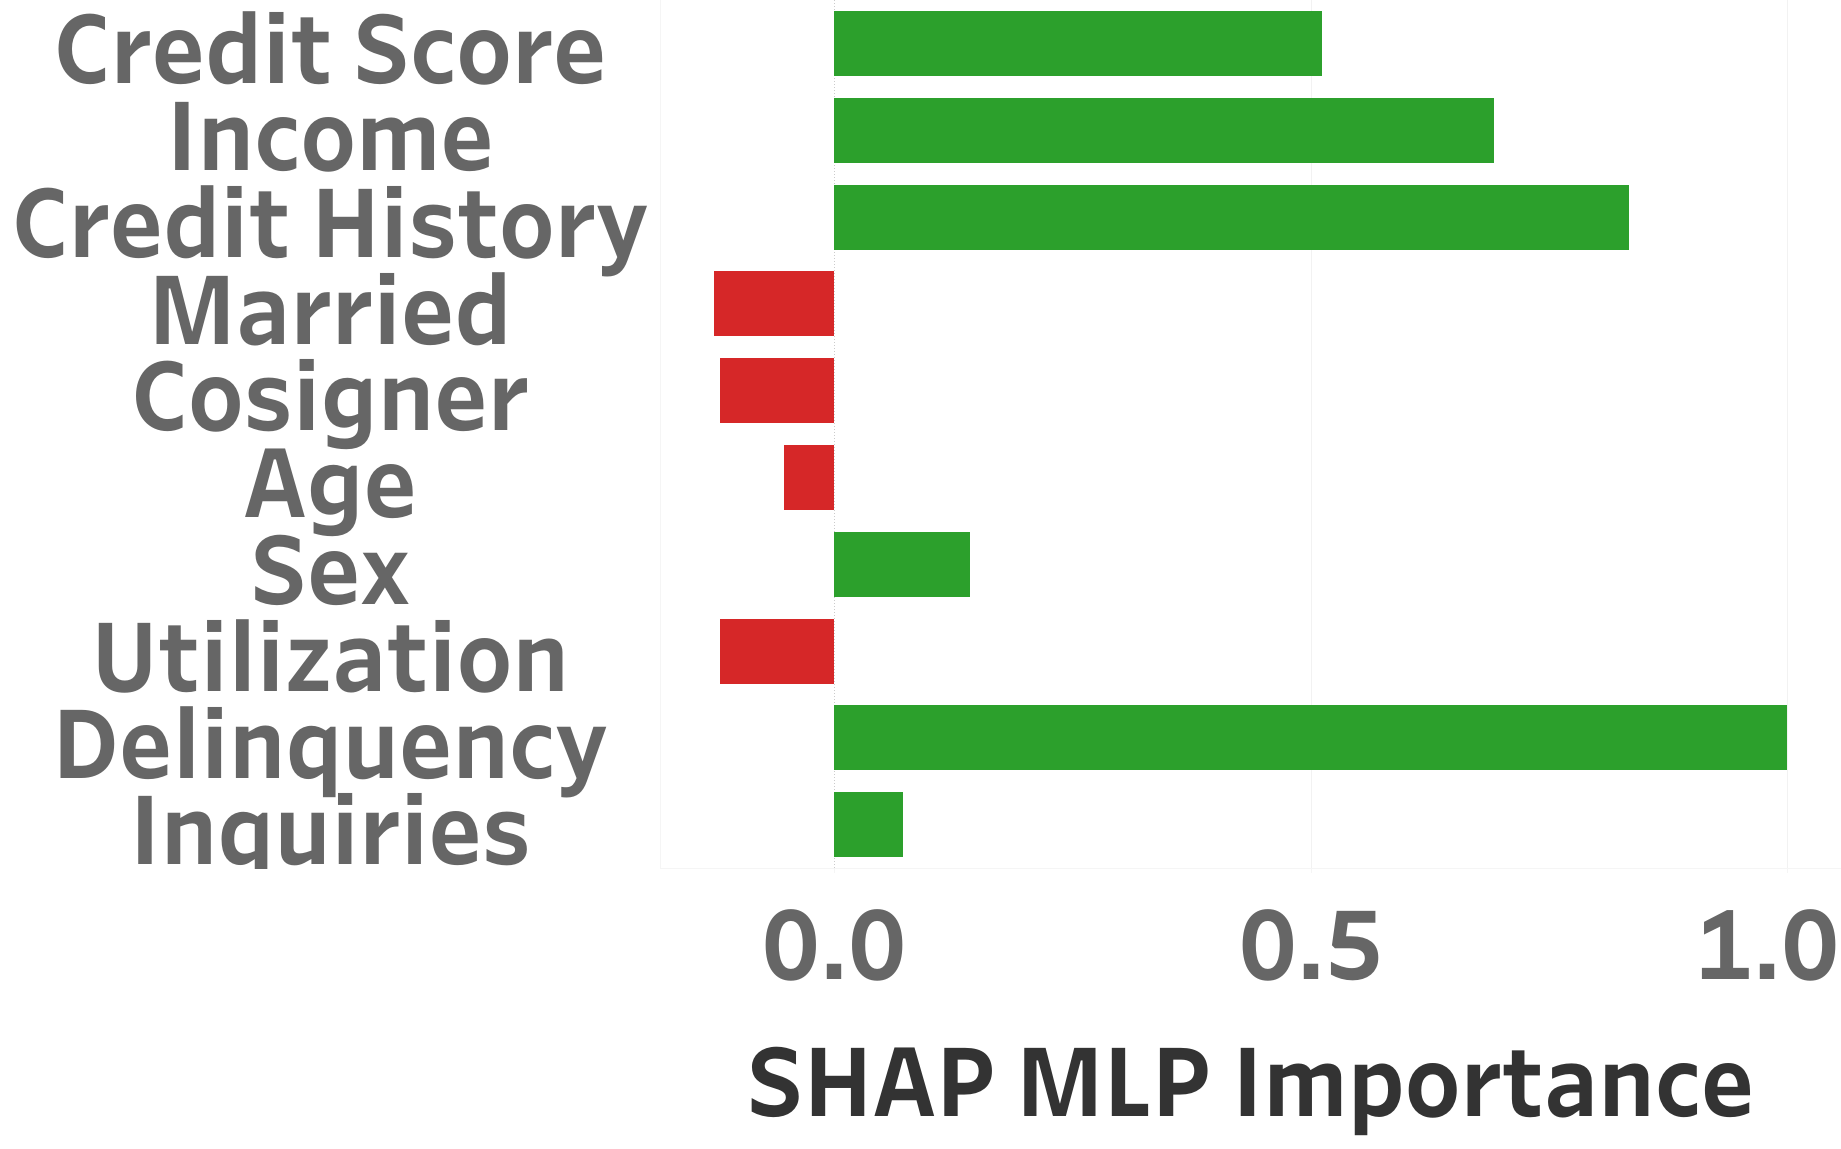
\includegraphics[width=0.65\linewidth]{Figs/shap_mlp_ex.png}%}%{Figures/feng_fig/acc_increase_size_2.png}
              \caption{SHAP's explanation of John's application decision}
              \label{fig:shap_ex}
            \end{subfigure}
        \caption{John's demographics along with a plot of the SHAP values obtained by explaining $\mathcal{M}$'s prediction for John. (b) quantifies the extents and directions with which SHAP says each feature is important to each class using a diverging bar chart. The numbers correspond to the SHAP coefficients $e_{\text{SHAP}}(x_j)$. The red bars represent negative contributions of $e_{\text{SHAP}}(x_j)$.}
        \label{fig:shap_ex_full}
        \end{figure}



 
% Figure \ref{fig:shap_ex} shows the output of LIME (using the Python LIME package) for the applicant. 
% REMOVED SO AS NOT TO SPOIL
% This explanation representation exemplifies one of the main criticisms of LIME mentioned in \citep{dieber20assessing}; it is unclear what the values associated to each feature in the rightmost part of the figure mean.
% John's feature values along with SHAP's explanation for his approval are visualized in Figure \ref{fig:shap_ex_full}. We denote them by $e_\text{SHAP}(x_j)$.% So even though credit inquries and income occur on different scales, their feature importance values are directly comparable and so their associated values of .09 in Figure \ref{fig:shap_ex} indicate that they are nearly tied to be the most important features in $\mathcal{M}$'s prediction for John. %Furthermore, income and credit inquiries both contribute .09 to the prediction that the applicant is approved. %increasing their credit score by one standard deviation would have increased the output of the ridge regressor by .034. 
% Overall, including the intercept term, the formula for the ridge regressor is as follows. We have abused notation by omitting any indication that the features are standardized. 
% \begin{gather*}
%     LIME(x)=.65 -.015 \cdot \text{Age} +.004\cdot \text{Sex} + .053 \cdot \text{Married} -.024 \cdot \text{Cosigner} + .036 \cdot \text{Credit history} \\+.085 \cdot \text{Income} -.030 \cdot \text{Utilization} -.058 \cdot \text{Delinquencies} - .094 \cdot \text{Inquiries} +.047 \cdot \text{Credit Score}
% \end{gather*}

% REMOVED SO AS NOT TO SPOIL
% The ground truth feature importance is represented by $\mathbf{\Sigma}_i$, where $\beta_i$ are the logistic regression coefficients from Equation 1.  $\beta_i$ are scale-agnostic feature importance measures because the logistic regression takes standardized data as input. $\beta_i$ measures how the odds of loan approval increases when feature $i$ is increased by one standard deviation. Since these coefficients are not directly comparable to LIME's feature coefficients $e_LIME}$ (logistic regression coefficients are interpreted in terms of odds while LIME's coefficients are interpreted in terms of the output of a ridge regressor), we instead compare the max-normalized sets of $\beta_i$ and $e_LIME}_i$. The feature importance values are max-normalized in order to emphasize how LIME and $\mathcal{G}$ compare in terms of relative feature importance.

 Following how post hoc explanations are interpreted in the literature, we now inspect the $e_\text{SHAP}(x_j)$ coefficients to try to infer some information about the marginal effect of each feature. First, we can use the sign of the coefficients to infer the directionality of the impact of features. For example, we may deduce that the negative SHAP coefficient of ``Married'' in Figure \ref{fig:shap_ex} implies that if the applicant is married, the likelihood of loan approval decreases. We could use this as evidence to infer that being married has a negative relationship with loan approval in reality. Second, we can use SHAP coefficients to make inferences about the relative importance of features. For example, the ``Delinquency" has the largest positive impact while ``Married" has the largest negative impact. Finally, we can use the magnitudes of the features to identify the most influential features. In this case, the ``Delinquency", ``Credit History" and ``Income" are the three most important features. %We use feature importance of $\mathcal{G}$ as the ground truth to compare with the feature importance generated by post hoc explanations since, in practice, users do not have access to $\mathcal{G}$. 

% \subsection{misalignment Within a Pipeline and Inconsistency Across Pipelines} 

We inspect the quality of the SHAP explanations by comparing the $e_\text{SHAP}(x_j)$ with the $\beta_j$, which governs the ground truth relationship between explanatory variables and the target variable. Feature importance according to SHAP and $\mathcal{G}$ are  shown in the left and middle plot (Pipeline 1) in Figure \ref{fig:shap_ex} respectively. Unfortunately, the explanations differ significantly from the true marginal effects in every way, not just in value, but even in sign and relative importance. For example, the most important feature (largest $\beta_j$) should be ``Credit Score'' but SHAP suggests ``Delinquency'' is the most important. In addition, being married should have a positive impact on getting a loan application approved and yet SHAP implies that the impact is negative. This example underscores the inherent pitfalls in relying on post hoc explanations to deduce marginal effects, offering a stark illustration of how their application can yield misleading interpretations. 

Beyond the evident misalignment, the inconsistency of the explanations further compounds the problem. Repeating the pipeline with alternative selections for $\mathcal{M}$ while maintaining all other parameters constant yields divergent SHAP explanations, as shown in the right plot of Figure \ref{fig:shap_ex}. These explanations vary greatly; the only point of agreement is that ``Credit Score" and ``Income" are important features assigned positive Shapley values. 

The ensuing sections will expand upon the risks associated with employing post hoc explanations to make inferences about marginal effects. We aim to provide a detailed theoretical foundation for their limitations and a thorough critique backed by empirical evidence, revealing the dangers of this approach.
%   We see from the difference in relative magnitudes of the coefficients from $e(x_j)$ in Figure \ref{fig:shap_ex} and the ground truth in Equation \ref{eqn:gt} that the explanation for John's approval is unfaithful.


%\subsection{Inconsistency Across Pipelines}
    % We simulate this scenario and show the results obtained by the two researchers in \ref{box}. We also compare the LIME explanations they receive with the ground truth. The plots at the bottom left, bottom middle, and bottom right show the importance of each feature. The features are vertically ordered from most to least important to $\mathcal{G}$. Feature importance values for the MLP and XGBoost models come from LIME's explanation of the models' decisions to approve John. They are max-normalized. The feature importance values for the ground truth are represented as the max-normalized coefficients of $\mathcal{G}$ from Equation \ref{eqn:gt}. We use max-normalization because the feature importance values of LIME and the coefficients of $\mathcal{G}$ occur on different scales. In the left and middle panels, the feature importance plots being visualized are for the ground truth and MLP from the previous section. For the right panel, we trained an XGBoost model with 3 estimators that achieves about an $85\%$ test set accuracy. Although they had similar accuracies, the MLP and XGBoost models may have captured different correlations in the data because the explanations of the MLP and XGBoost models were quite different from each other. The explanations of both black boxes were unfaithful and both had distinct errors (otherwise all three feature importance plots would look nearly identical). To see this, note that in pipeline 1 credit inquiries are implied to be the most important even though credit score is actually the most important. Also note that although credit score was correctly identified as the most important in pipeline 2, all the other features, except income, were incorrectly implied to be negligible. The explanations of pipelines 1 and 2 are also contradictory in that in pipeline 1 being male (sex$=1$) has a positive impact on approval chances while in pipeline 2 being male has a negative impact. 
     
\settowidth\mylenC{\textbf{$\mathcal{M}=\text{\textbf{XGBoost}}$}} 
% determine usable width of cols 2 and 3:
\setlength\mylenD{(.3\linewidth-3\tabcolsep)/3}


\begin{tcolorbox}[tabular = {*{9}{wc{\mylenD}}}, hbox,center,label = {pipelines_3_ex}]
\\%\midrule
\noalign{\vspace{-\normalbaselineskip}}
%\multicolumn{2}{c}{} & \multicolumn{2}{c}{$\mathcal{E}=\text{\textbf{LIME}}$}  & \multicolumn{2}{c}{$\mathcal{E}=\text{\textbf{LIME}}$} \tabularnewline \midrule
\multicolumn{3}{c}{\textsc{$\mathcal{G}$}} & \multicolumn{3}{c}{\textsc{Pipeline 1: }$\mathcal{M}=\text{\textsc{MLP}}$}  & \multicolumn{3}{c}{\textsc{Pipeline 2: }$\mathcal{M}=\text{\textsc{XGBoost}}$} \tabularnewline \cmidrule(lr){1-3}\cmidrule(lr){4-6}\cmidrule(lr){7-9}%\midrule
\multicolumn{3}{c}{\textsc{Ground Truth}} &\multicolumn{1}{wc{\mylenD}}{$\mathcal{E}$} & \multicolumn{1}{wc{\mylenD}}{\textsc{Accuracy}} & \multicolumn{1}{c}{\textsc{AUC}} & \multicolumn{1}{wc{\mylenD}}{$\mathcal{E}$} &\multicolumn{1}{wc{\mylenD}}{\textsc{Accuracy}} & \multicolumn{1}{wc{\mylenD}}{\textsc{AUC}}\tabularnewline\midrule
 & & & \multicolumn{1}{wc{\mylenD}}{SHAP} &\multicolumn{1}{wc{\mylenD}}{.86} & \multicolumn{1}{wc{\mylenD}}{.93} & \multicolumn{1}{wc{\mylenD}}{SHAP} &\multicolumn{1}{wc{\mylenD}}{.86} & \multicolumn{1}{wc{\mylenD}}{.97}\tabularnewline %\midrule
\multicolumn{3}{c|}{\begin{minipage}{.3\textwidth}
      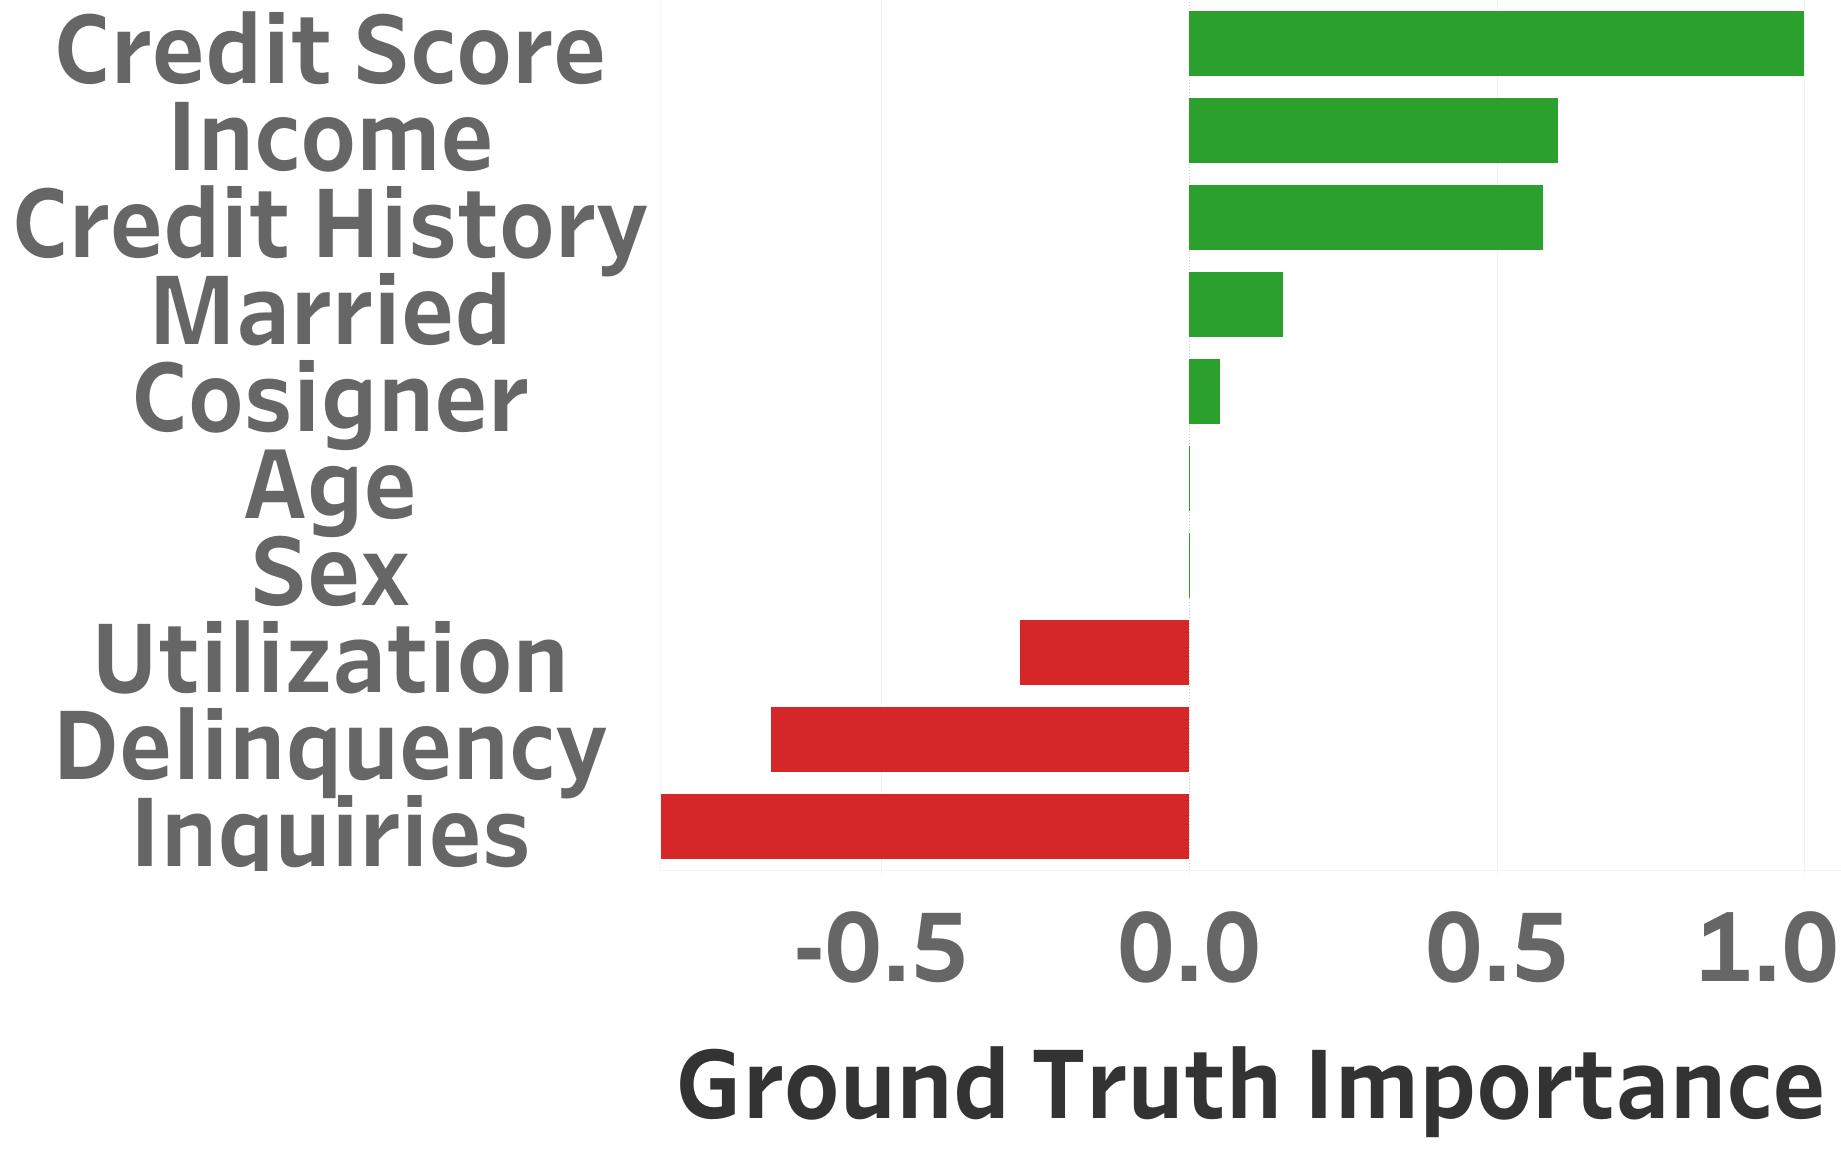
\includegraphics[width=\linewidth]{Figs/g_ex.png}
    \end{minipage}} & \multicolumn{3}{c}{\begin{minipage}{.3\textwidth}
      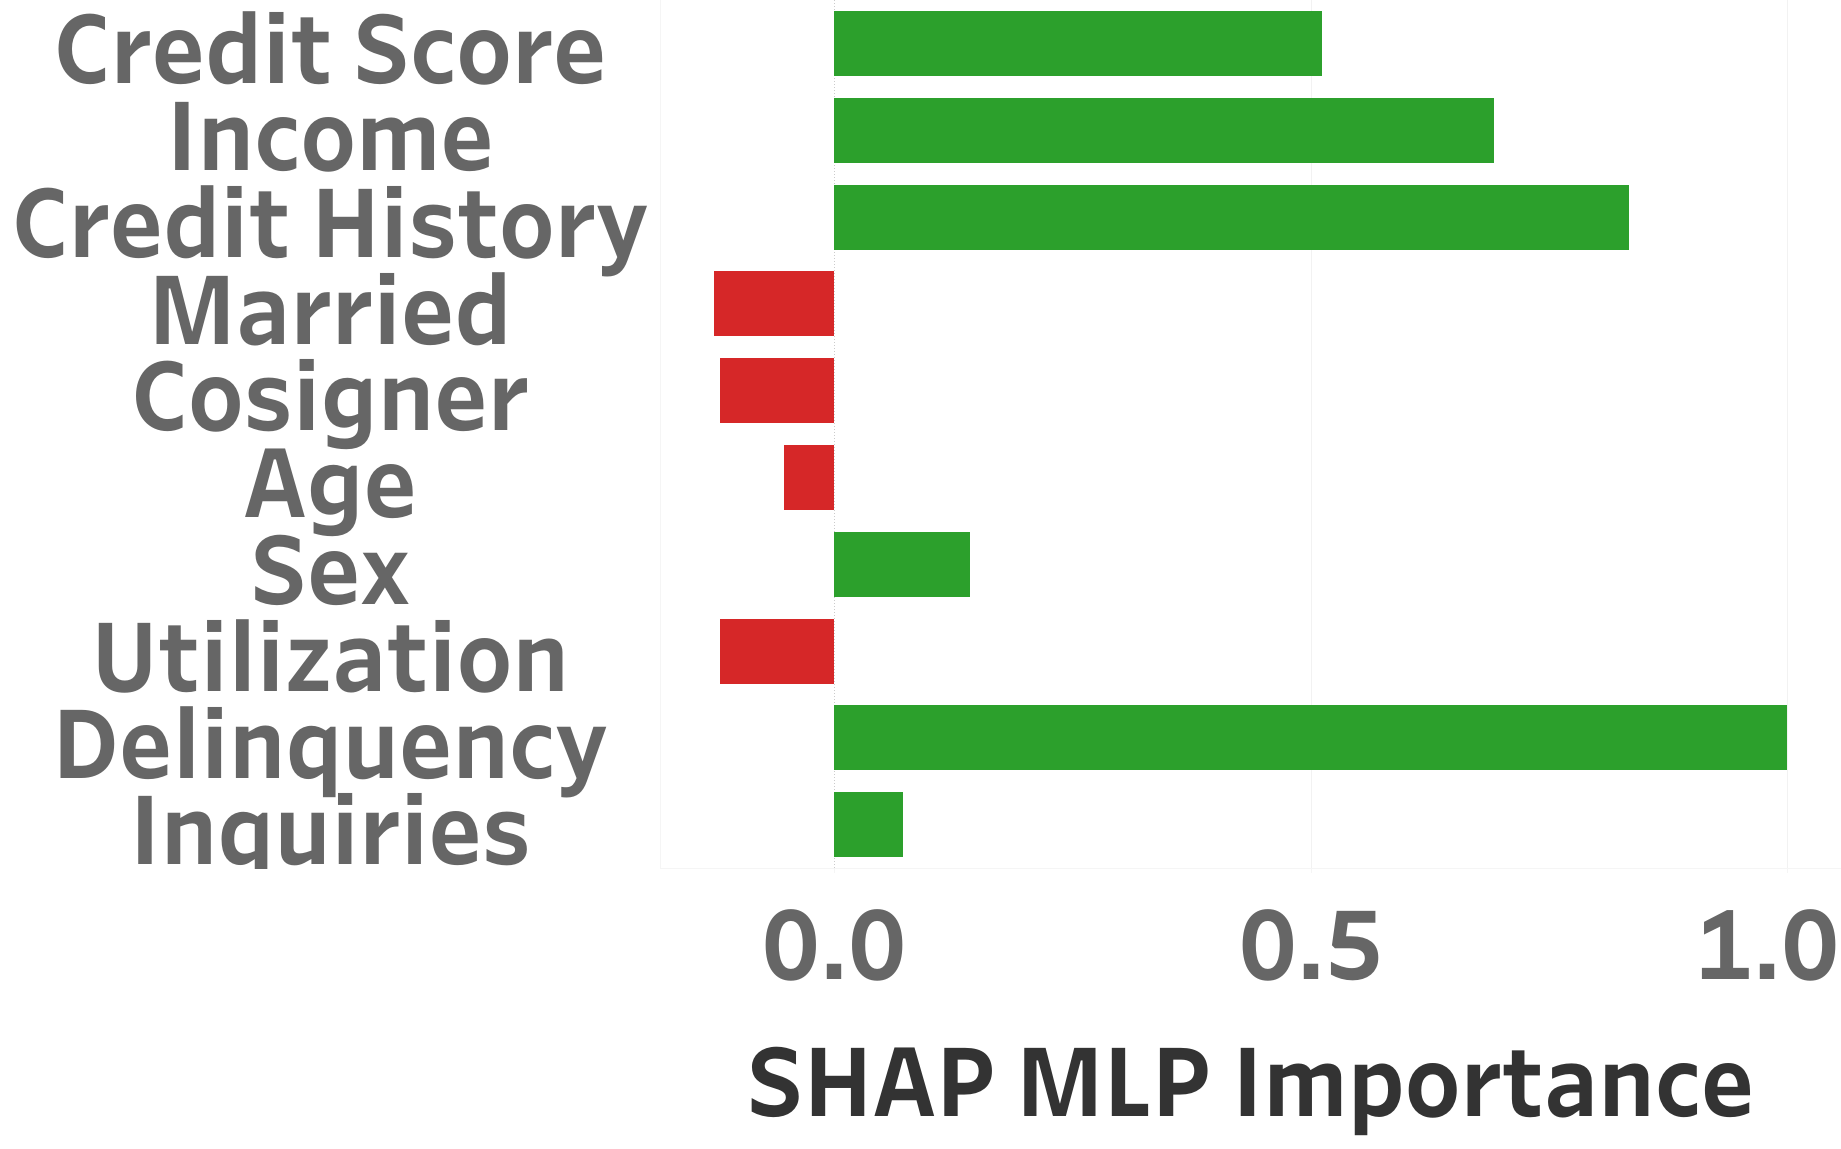
\includegraphics[width=\linewidth]{Figs/shap_mlp_ex.png}
    \end{minipage}}  & \multicolumn{3}{c}{\begin{minipage}{.3\textwidth}
      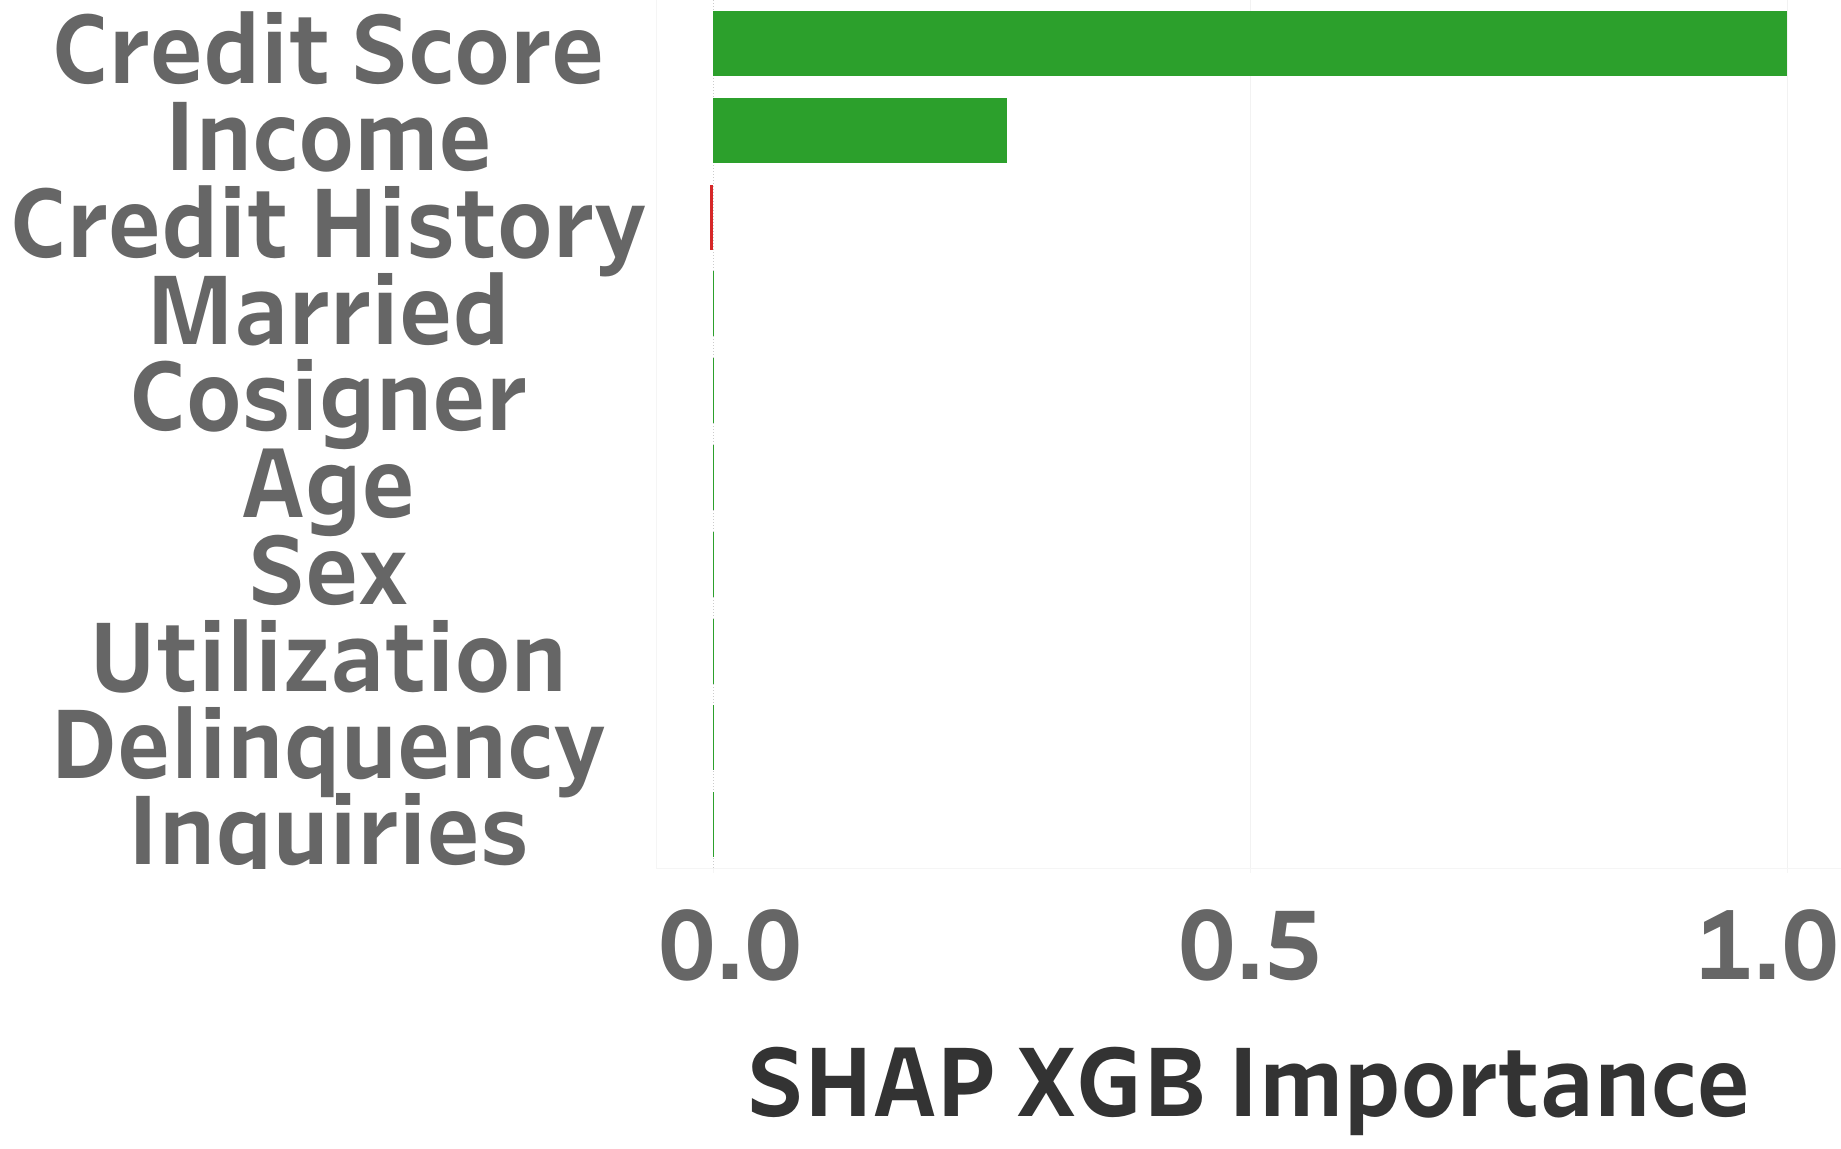
\includegraphics[width=\linewidth]{Figs/shap_xgb_ex.png}
    \end{minipage}} \tabularnewline \midrule
\end{tcolorbox}
\noindent\begin{minipage}{\textwidth}
\captionof{figure}{Ground truth feature importance along with qualitatively different explanations for John obtained when using four instances of the pipeline. In the first pipeline, SHAP is used to explain an MLP. In the second pipeline, SHAP is used to explain an XGBoost model with similar performance. Feature importances are illustrated using diverging bar charts. }\label{box}
\end{minipage}

The concrete demonstration of the \textit{misalignment} and \textit{inconsistency} of post hoc explainers in Figure \ref{box} motivates the main thrust of this paper. That is, we want to find out why post hoc explainers are misaligned and inconsistent, what resulting harm could be done to researchers using such explainers, and what mitigation strategies could be applied. %Section \ref{sec:misalignment} compiles evidence that certain properties of the training data, explainer, and black box are related to how unfaithful explanations are, uses that evidence to motivate mitigation strategies for misalignment, and finally tests those strategies. Section \ref{sec:inconsistency} is similar in structure but addresses inconsistency instead of misalignment.
% \begin{figure}[ht!]
% \centering
%     \begin{subfigure}[b]{.3\textwidth}
%           \centering
%           \includegraphics[width=\textwidth]{Figures/lime_G.png}%{Figures/feng_fig/lime_0_v1.png}
%           \caption{Default LIME explanation of $\mathcal{G}$}
%           \label{fig:lime_G}
%     \end{subfigure}%
%     \hfill
%     \begin{subfigure}[b]{.3\textwidth}
%           \centering
%           \includegraphics[width=\linewidth]{Figures/lime_seed_320.png}%{Figures/feng_fig/shap_0_v1.png}
%           \caption{Lime with seed 320 explanation of an MLP}
%           \label{fig:lime_seed_320}
%     \end{subfigure}
%     \hfill
%     \begin{subfigure}[b]{.3\textwidth}
%           \centering
%           \includegraphics[width=\textwidth]{Figures/lime_M_XGB.png}%{Figures/feng_fig/shap_0_v1.png}
%           \caption{Default LIME explanation of an XGBoost}
%           \label{fig:lime_xgb}
%     \end{subfigure}
% \caption{Proof that LIME can give different explanations that are incorrect in different ways. On the left, LIME correctly ranks the features when explaining $\mathcal{G}$. It can also do this when explaining an MLP, unless it has an unfortunate choice of random seed (middle). LIME's explanation of an XGBoost model with close to the same accuracy as the MLP is somehow even more unfaithful.}
% \label{fig:lime_inconsistency}
% \end{figure}

% REMOVED TO FOCUS ON DESCRIPTIVE
% \subsection{Prescriptive Insight}
% \label{sec:prescriptive}
%      Now we demonstrate a simple way to leverage LIME to obtain guidance for denied applicants who would like to be approved in the future. We produce counterfactuals with LIME by simply perturbing the most important feature it identifies. This time, we consider another applicant whose loan application is rejected and check if LIME can provide effective guidance for how to make the applicant's next application be approved. The applicant in question is a 39-year-old married male who has a ``cosigner", a credit score of 672, and makes \$38,771/year. They have a 20-month-old line of credit, use 20\% of their total credit, have had 5 credit inquiries in the past 6 months, and it has been 21 months since their last delinquent payment. Figure \ref{fig:lime_negative_ex} shows LIME's feature importance values for the denied applicant. LIME implies that the top three most important factors for their rejection were their number of recent credit inquiries, income, and the time since the last delinquent payment. We suppose that the individual would like to just wait some time for their credit inquiries to disappear off of their report, but does not know how many of the five inquiries they have that they need to erase. Manual perturbation of the number of credit inquiries showed that $\mathcal{M}$ would accept their application if their number of credit inquiries is reduced by at minimum two standard deviations. However, even setting the number of credit inquiries to zero does not yield an application that $\mathcal{G}$ would accept. 
    
%     % Of these three, the applicant would only view credit score as actionable. Because LIME's surrogate model has a coefficient of $-.23$ for credit score, LIME implicitly suggests that the individual should lower their credit score in order to be approved. We can check if $\mathcal{M}$ defies intuition by modeling credit score as having a negative relationship with loan approval probability by decrementing the credit score from 672 to, say, 550. Doing this fails to change the output of $\mathcal{M}$ and highlights another key deficiency of LIME: it doesn't actually tell us about how $\mathcal{M}$ uses the features internally. So we are forced to adopt one of the following two assumptions. Either that $\mathcal{M}$ is modeling an unintuitive relationship or that LIME is wrong. In practice $\mathcal{G}$ is of course unknown and $\mathcal{M}$ is still a black-box, so neither assumption is testable. It turns out that, in this case, we have to raise the credit score to at least 762 and lower the number of inquiries to at most 2 for the individual to be approved (by $\mathcal{M}$). Increasing the credit score and lowering the inquiries are the opposite of what LIME's feature importance signs suggested. %So, in this case, LIME just poses more questions instead of providing a definitive prescriptive insight. 

% In the next two sections, we will investigate and show evidence why post hoc explainers could lead to wrong descriptive and prescriptive insights. Specifically, we focus on two aspects of post hoc explanations, namely, the \textit{incorrectness} and \textit{inconsistency}.   The following subsections document various vulnerabilities in these two aspects post hoc explainers have and how they could cause business researchers to misunderstand a business process. 


% \begin{figure}[ht!]
%     \centering
%     \includegraphics[width=.48\textwidth]{Figures/lime_negative_ex.png}
%     \caption{LIME's explanation for a rejected applicant used in Section \ref{sec:prescriptive}. LIME identifies income, credit score, and credit inquiry count as the top three most important features.}
%     \label{fig:lime_negative_ex}
% \end{figure}




    %We also use the $L_2$ distance between the vectors of feature importance values to evaluate explanation instability. This is motivated by our desire to seek conditions associated with explanations for the outcomes of applicants with similar profiles being very different (i.e. unstable).  


\section{Misalignment of Post Hoc Explanations}
  In this section, we study a most important question: Do post hoc explanations of a model $\mathcal{M}$ provide correct information about the true marginal effects of features in $\mathcal{G}$? We first describe how we evaluate explanations in Section \ref{sec:evaluating_faithfulness}. 
  Then, in Section \ref{sec:causes_of_misalignment}, we identify properties of the data $\mD$, the model $\mM$, and the explainer $\mE$ used in a pipeline that lead to misaligned explanations and demonstrate how those individually affect the explanation. Finally, we adduce the generality of the problem of misalignment in Section \ref{sec:pervasive}. %%The experiments in this section all use our running example of explaining loan application decisions, where the ground truth model is a linear model. 

\subsection{Metrics for Assessing the Data-Alignment of Explanations}
   \label{sec:evaluating_faithfulness}
  Both SHAP and LIME provide a feature importance for each feature $j$, denoted by $e_\mE(x^{(i)}_j)$, where $\mE$ represents the explainer. 
   Our goal is to investigate whether $e_\mE(x^{(i)}_j)$ can be used to provide correct information about the marginal effect of feature $j$, in terms of three different aspects motivated by practical use cases of explanations from the literature: the sign, the importance ranking, and relevance. 
     
     First, we give a more detailed definition of the true marginal effects $\boldsymbol{\beta}$ (with some simplifying assumptions) so that our estimand is clear. Our characterization of $\boldsymbol{\beta}$ captures both the correlative effect that each explanatory variable has on the response variable individually as well as any effects that one variable can have on the target through other variables that depend on it. This is accomplished by considering two cases in our definition. If a feature $X_j$ does not depend on any other feature, we define $\beta_j$ to be the total derivative $\dv{Y}{X_j}$. Otherwise, we define $\beta_j = \pdv{Y}{X_j}$. 



         
         % The metrics we propose are motivated by how the post hoc feature importances are used in business research.
          We design three metrics to evaluate data-alignment from different angles considering the practical use case of the explanations. Researchers using SHAP and LIME typically use the feature importance values in three main ways: 1) inspect the sign of the feature importance values to identify how the features impact the outcome they are interested in; %For example, in \citep{park2024extracting} says that the quad-core feature of smartphones having a negative SHAP value also indicates a negative effect on consumer choices. 
         2)  identify the relative importance of features %This type of analysis is exemplified in \citep{zhang2023explainable}, which advocates for managers to use the top most important features from the ranking they obtained via SHAP as early indicators of financial risk in manufacturing companies. 
         and 3) identify the most influential features. %cite kovvuri
    %To capture how well SHAP and LIME can do these things, we use three metrics. 

    The first metric, termed \textbf{directionality}, measures whether post hoc explainers can at least identify the correct \textit{sign} of a feature's influence on the outcome. It evaluates an explanation only qualitatively. We calculate directionality by determining the percentage of cases where the sign of $e_\mE(x^{(i)}_j)$ matches that of $\beta_j$ for each feature $j$ across $m$ instances in the test set. %However, when $\beta_j$ is sufficiently small, checking the sign agreement would be too strict. Thus, we relax the definition and instead check if $\mid e_\mE(x^{(i)}_j)\mid $ is also very small relative to the largest feature importance value $\max_{j^\prime} \mid e_\mE(x^{(i)}_{j^\prime}) \mid $.
    % Given the ground truth $\beta_j$ and feature importance values $e_\mE(x^{(i)}_j)$ from an explainer, we denote the accuracy for the $j^{\text{th}}$ feature as follows. 
    % Note that this definition is  made in reference to the entire test set $\{x^{(i)}\}_{i=1}^n$ but considers only one feature index $j$.  %The notation $\hat{\beta}^{(i)}$ represents a feature importance vector for the $i^{\text{th}}$ test set instance. 
    \begin{equation}
        \label{eq:acc}
        \texttt{directionality}(\{e_\mE(x^{(i)}_j)\}_{i=1}^m,\beta_j) = \frac{1}{m} \sum_{i=1}^m s_j( e_\mE(x^{(i)}_j),\beta_j)
    \end{equation}
    where 
    \begin{equation*}
        s_j(e_\mE(x^{(i)}_j),\beta_j) = \begin{cases*}
                    \mathbf{1}_{\mathbb{R}^+}(\beta_j \cdot e_\mE(x^{(i)}_j)) & if  $\mid \beta_j\mid > \epsilon_1$  \\
                     \mathbf{1}_{(0,\epsilon_2)}\left(\frac{\mid e_\mE(x^{(i)}_j)\mid }{\max_{j'} \mid e_\mE(x^{(i)}_{j'})\mid}\right) & otherwise
                 \end{cases*}
    \end{equation*}
    Here $\mathbf{1}_S(z)$ is an indicator function that returns 1 if $z\in S$ and outputs 0 otherwise. $s_j(e_\mE(x^{(i)}_j),\beta_j)$ is designed to facilitate a relaxed version of accuracy by checking if  $\beta_j$ and $e_\mE(x^{(i)}_j)$ have the same sign only when $\beta_j$ is not very small, i.e. larger than $\epsilon_1$. When $\beta_j$ is small, $s_j$ instead checks if $e_\mE(x^{(i)}_j)$ is small relative to the other $e_\mE(x^{(i)}_{j^{\prime}})$, $j\prime \neq j$. The ratio of $\mid e_\mE(x^{(i)}_j)\mid $ and $\max_j^\prime \mid e_\mE(x^{(i)}_{j^\prime})\mid$ should be small, i.e. at most $\epsilon_2$.
    In our experiments, we use $\epsilon_1=1e-2$ and $\epsilon_2=1e-2$. 
    
      The second metric, \textbf{concordance}, measures how accurately the explanations recover the \textit{relative importance} of features compared to the ground truth, $\beta_j$. Given the $e_\mathcal{E}(x^{(i)}_j)$, we rank the features from least to most important and calculate the \emph{Spearman Rank Correlation} \cite{spearman1904proof} between this ranking and a ranking of the $\beta_j$. While the directionality metric is computed using the entire test set per feature, the concordance is computed per instance using all features.

    % The Spearman rank correlation is defined as follows. 
    \begin{equation}
       \texttt{concordance}(e_\mE(\mathbf{x}^{(i)}),\boldsymbol{\beta}) = 1 - \frac{6\sum_{j=1}^d (\text{rank}(\beta_j) - \text{rank}(e_\mE(x^{(i)}_j)))^2}{d(d^2-1)},
    \end{equation}
    where $d$ is the number of features, and $\text{rank}(\beta_j)$ and $\text{rank}(e_\mE(x^{(i)}_j))$ denote the rank of the $j^{\text{th}}$ feature according to the coefficients of $\boldsymbol{\beta}$ and explanations $e_\mE(\mathbf{x}^{(i)})$, respectively. If the explainers' rankings are 100\% correct, then the correlation should be 1. Any value less than 1 indicates an error in the rankings, leading users to misinterpret the importance of some features.
    
Third, motivated by the fact that  researchers may only be  interested in identifying a small set of features that have the biggest impact, we define the third metric, \textbf{relevance}, based on the ranking of features. Our metric, denoted $\text{relevance}_k$, measures how many of the top-$k$ most important features identified by $\mathcal{E}$ are indeed among the top-$k$ largest marginal effects. Denote by $I_k^+(e_\mE(\mathbf{x}^{(i)}))$ and $I_k^+(\boldsymbol{\beta})$  the set of feature indices  among the top-$k$ most highly ranked according to $e_\mE(\mathbf{x}^{(i)})$ and $\boldsymbol{\beta}$, respectively. Then we define 
    \begin{equation}
        \texttt{relevance}_k(e_\mE(\mathbf{x}^{(i)}), \boldsymbol{\beta}) = \frac{\mid I_k^+(\boldsymbol{\beta}) \cap I_k^+(e_\mE(\mathbf{x}^{(i)}))\mid}{k}.
    \end{equation}
     Like the concordance metric, $\text{relevance}_k$ is also computed at the instance level. 
    In our experiments, we compute $\text{relevance}_k$ for each $k$ and plot the means and standard errors over $m$ instances. $\text{relevance}_k(e_\mE(\mathbf{x}^{(i)}), \boldsymbol{\beta})$ represents the true positive rate for the identification of what features are among the top-$k$ largest marginal effects according to $\mathcal{E}$.       
    
   
        




 \paragraph{Data-Alignment Evaluation}
  We call the evaluation of the directionality, concordance, and relevance the evaluation of \textbf{data-alignment}. We evaluate the data-alignment
 for SHAP and LIME on $m=100$ applicants randomly selected from the test set and report the results in Figure \ref{fig:beta_alignment}. 
 We find that neither SHAP or LIME achieves satisfying results on any of the three dimensions. Particularly, SHAP, while strongly favored over LIME by researchers, perform significantly worse than LIME in all three dimensions. SHAP cannot even identify the correct directionality of the features, let alone the concordance. To have a better understanding of SHAP, we also simulate a \emph{random} explainer that randomly draws its feature importance values $e_\text{random}(x^{(i)}_j)$ from a standard normal distribution for each $j$ and $i$. We find that \emph{SHAP explanations do not have better data-alignment than random explanations do with respect to directionality and concordance.}         
                    \begin{figure}[ht!]
            \centering
            \begin{subfigure}[t]{.28\textwidth}
              \centering
              \captionsetup{justification=centering}
                  \raisebox{.2cm}{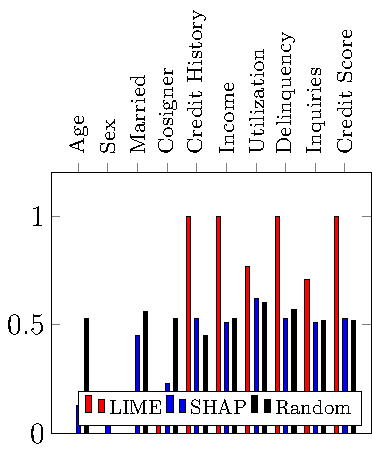
\includegraphics[width=\textwidth]{Figs/sec4_1-figure0.pdf}}%{Figures/lime_shap_Spearman_magnitude.png}

              \caption{Directionality}%Spearman rank correlations of feature importance magnitudes from SHAP and LIME against the true ranking from $\mathcal{G}$. }
               \label{fig:lime_shap_sign_accs}
            \end{subfigure}%
            \hspace{1cm}%\hfill
            \begin{subfigure}[t]{.28\textwidth}
              \centering
               \captionsetup{justification=centering}
              \raisebox{.05cm}{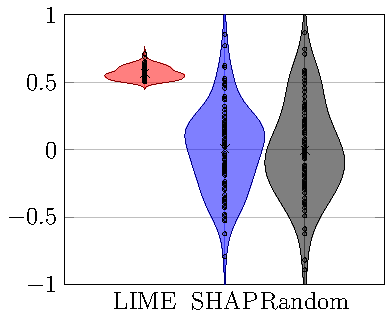
\includegraphics[width=\textwidth]{Figs/sec4_1-figure1.pdf}}%{Figures/lime_shap_Spearman_signed.png}
              \caption{Concordance}%Spearman rank correlations of signed feature importance from SHAP and LIME against the true ranking from $\mathcal{G}$.}
               \label{fig:lime_shap_Spearman_signed}
            \end{subfigure}
            \hspace{1cm}%\hfill
            \begin{subfigure}[t]{.28\textwidth}
              \centering
               \captionsetup{justification=centering}
            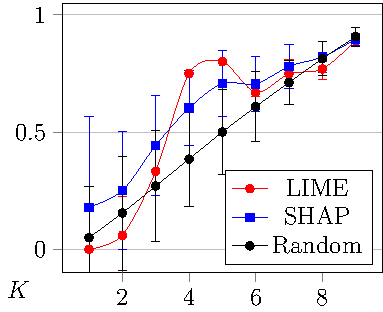
\includegraphics[width=\textwidth]{Figs/sec4_1-figure2.pdf}%
            \caption{Relevance}%The average and standard error of recall of SHAP and LIME when attempting to capture the top K most important features to $\mathcal{G}$ when explaining $\mathcal{M}$, for varied $K=1,2,3,...$ number of features.}
            \label{fig:avg_recall}
            \end{subfigure}
            \caption{Bar plot of directionality, violin plot of concordance, and line plot for relevance$_k$. For plot (c) Each point in the line plot represents a mean relevance for a given $k$. The error bars represent the standard error. The total number of features is 10.}
           \label{fig:beta_alignment}
        \end{figure}    
  
    \subsection{Contributing Factors to  Misalignment}
        \label{sec:causes_of_misalignment}
        Having demonstrated that SHAP and LIME explanations have poor data-alignment, we now move on to investigate factors in the pipeline that contribute to the misalignment. We aim to provide both theoretical and empirical evidence for why post hoc explanations should not be used to infer marginal effects. We first investigate the models of SHAP and LIME in the explanation stage to show why their model design contribute to misalignment. We work under the assumptions that domain knowledge about the data generation process is unavailable and therefore address the key factors in the prediction stage that researchers actually have control over. Namely, how training data are prepared and how $\mathcal{M}$ and $\mathcal{E}$ are constructed.% and how $\mathcal{M}$'s training data are pre-processed. 


    \subsubsection{Explainer Estimands Are Not Necessarily $\beta$}
    \label{sec:theoretical_considerations}
   We first investigate how the explainers themselves contribute to misalignment by deriving and analyzing equations for their explanations. To exclude other factors in the explanation pipeline, we assume here that we have access to the ground truth model $\mathcal{G}$ and that SHAP and LIME are directly applied to explaining $\mathcal{G}$. Thus, the explanations solely depend on the explanation stage. We suppose that $\mathcal{G}$ is a linear function of $d$ features and SHAP and LIME explain the output of $\mathcal{G}$ at a point $\boldsymbol{\xi}$, that is, $\mathcal{G} = \boldsymbol{\beta}^T \mathbf{x}$ where $\mathbf{x} \sim \mathcal{N}(\mathbf{0},\mathds{1}_d)$ and $\boldsymbol{\xi}$ is a realization of $\mathbf{x}$. Below we derive mathematical representations of SHAP and LIME explanations, and investigate their relationships with $\boldsymbol{\beta}$.

         \paragraph{$e_{\text{SHAP}}$ when Explaining a Linear Model}
              %SHAP does \emph{not} recover $\boldsymbol{\beta}$ and should not be relied upon for this purpose. 
              The importance of the $j^{th}$ feature of the $i^{th}$ data sample $\xi^{(i)}_j$ in a SHAP explanation is the Shapley value for that feature in that sample. The Shapley value reduces to the following expression when SHAP is used to explain a linear model according to \cite{StrumbeljErik2014Epma,lundberg17shap}. 
             \begin{equation}
                \label{eqn:shap_gt}
                e_\text{SHAP}(\mathbf{x}^{(i)}_j) = \beta_j (\xi^{(i)}_j - \bar{x}_j).
             \end{equation}

            
The SHAP explanations outlined by Equation \ref{eqn:shap_gt} exhibit several undesirable properties that can limit their practical application. For instance, when $\boldsymbol{\xi}=\bar{\mathbf{x}}$, the SHAP values $e_\text{SHAP}$ reduce to 0, leading to all features being deemed unimportant. Moreover, Shapley values cannot be used to infer the signs of the marginal effects because when $\xi^{(i)}_j - \bar{x}_j$ is negative, the signs of $e_{\text{SHAP}}(\xi^{(i)}_j)$ and $\beta_j$ are opposite. Additionally, it is derived from Equation \ref{eqn:shap_gt} that the expected SHAP values average to zero, rendering them generally uninformative about the marginal effects. Some authors address this in their search for global feature importance by instead considering empirical averages of absolute SHAP values \cite{lenaers23rent,maeng23vr,guenther2023useful}. However, this obviously comes at the cost of losing information about the directionality of a feature's impact.

             Following Equation \ref{eqn:shap_gt}, we propose to instead use normalize SHAP values: $e_{\text{SHAP}}(\xi^{(i)}_j) / (x^{(i)}_j - \bar{x}_j)$. We refer to these as \emph{normalized shapley values}. Although this is a straightforward adjustment one can make to in order to approximate the marginal effects using SHAP, we are not aware of it being used in prior literature.  Our empirical evaluation of these normalized Shapley values, which includes recalculating directionality, concordance, and comparison with traditional SHAP results (illustrated in Figures \ref{fig:beta_alignment} and \ref{fig:shap_dividex_corr}), suggests significant improvements. Normalized SHAP values frequently exhibit correct sign alignment and generate feature rankings highly concordant with ground truth. Directionality for features related to credit score improved remarkably, as shown in Figure \ref{fig:shap_dividex_accs}. However, directionality for the features related to cosigner (married and cosigner) possession decreased somewhat. The improvement to feature rankings are evident from Figures \ref{fig:shap_dividex_spearmans} and \ref{fig:shap_dividex_recalls}; we can see that mean concordance rose from near 0 to about .6 and relevance was improved substantially for $k=2,3,4,5$. 
             
            
             Given the demonstrated effectiveness of the SHAP normalization scheme and our evidence that unmodified SHAP explanations are so inherently data-misaligned such that they are comparable to random explanations, \textbf{we will adopt this normalization approach for all subsequent experiments detailed in this paper}. This is vital as we explore the impacts of $\mathcal{M}$'s predictive performance and feature independence in subsequent sections (\ref{sec:role_of_predictive_power} and \ref{sec:role_of_correlation}). %For example, we will use it in the following subsections on the roles of $\mathcal{M}$'s predictive performance and feature independence (\ref{sec:role_of_predictive_power} and \ref{sec:role_of_correlation}). We wish to show that increasing the predictive performance of $\mathcal{M}$ and using independent training data features may increase data-alignment, so the normalization scheme is necessary because otherwise SHAP's explanations are similar to random ones and thus will be unaffected by external effects. 
           \begin{figure}[ht!]
            \centering
            \begin{subfigure}[t]{.28\textwidth}
              \centering
              \captionsetup{justification=centering}
                  \raisebox{.2cm}{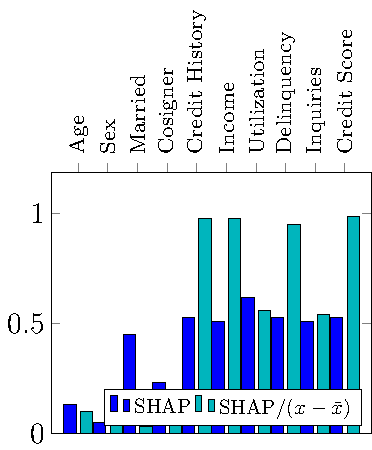
\includegraphics[width=\textwidth]{Figs/sec4_1-figure3.pdf}}%{Figures/lime_shap_Spearman_magnitude.png}

              \caption{Directionality}%Spearman rank correlations of feature importance magnitudes from SHAP and LIME against the true ranking from $\mathcal{G}$. }
               \label{fig:shap_dividex_accs}
            \end{subfigure}%
            \hspace{1cm}%\hfill
            \begin{subfigure}[t]{.28\textwidth}
              \centering
               \captionsetup{justification=centering}
              \raisebox{.05cm}{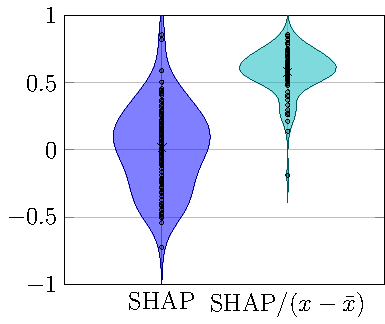
\includegraphics[width=\textwidth]{Figs/sec4_1-figure4.pdf}}%{Figures/lime_shap_Spearman_signed.png}
              \caption{Concordance}%Spearman rank correlations of signed feature importance from SHAP and LIME against the true ranking from $\mathcal{G}$.}
               \label{fig:shap_dividex_spearmans}
            \end{subfigure}
            \hspace{1cm}%\hfill
            \begin{subfigure}[t]{.28\textwidth}
              \centering
               \captionsetup{justification=centering}
            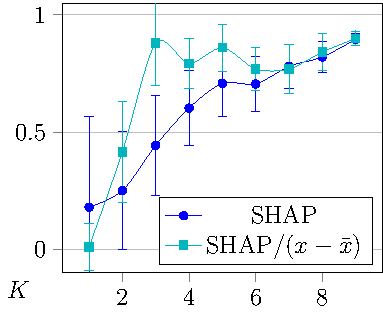
\includegraphics[width=\textwidth]{Figs/sec4_1-figure5.pdf}%
            \caption{Relevance}%The average and standard error of recall of SHAP and LIME when attempting to capture the top K most important features to $\mathcal{G}$ when explaining $\mathcal{M}$, for varied $K=1,2,3,...$ number of features.}
            \label{fig:shap_dividex_recalls}
            \end{subfigure}
            \caption{Comparison of SHAP explanations without and with SHAP value normalization}
           \label{fig:shap_dividex_corr}
        \end{figure}   
        \paragraph{$e_{\text{LIME}}$ when Explaining a Linear Model}
            \label{sec:lime_linear_case}
             %In this section we we will show that there are conditions when the LIME coefficients have the property $e(x_j)\simeq \beta$ and use this fact to justify that  $e(x_j)$ can be evaluated with respect to the ground truth $\boldsymbol{\beta}$. Those conditions are discussed in the next paragraph. 
             Local Interpretable Model-agnostic Explanations works by sampling data points around a given instance, then using these samples to train a weighted linear model as a local surrogate model that approximates the predictions of the original complex model in the vicinity of the instance. To obtain interpretable and sparse explanations, LIME incorporates  discretizes numeric features and includes a regularization component to promote sparsity in the local surrogate models it creates. This regularization helps in selecting a subset of features that are most influential for predictions near the instance being explained, thus ensuring that the explanations are both interpretable and concise. However, the above aspects of LIME's design may compromise its ability to accurately recover the true marginal effects coefficients. 
             
             The use of discretized features in the regression model can eliminate critical information about the decision boundary of the model being explained. Additionally, LIME's reliance on ridge regression incorporates a sparsity penalty, which may lead to zeroing out coefficients for features where $\beta_j$ is indeed non-zero, distorting the picture one may obtain of the marginal effects. Moreover, employing weighted ridge regression introduces a weight matrix that further skews the estimation of marginal effects. This distortion can be observed in the closed-form solution of the weighted ridge regression, indicating potential limitations in LIME's ability to provide accurate estimates under certain conditions.
             
             Thus, the aforementioned  considerations need to be overcome in order to get data-aligned explanations from LIME. Therefore, we propose a few theoretical results which show how LIME's hyperparameters govern its behavior and enable recovery of marginal effects. Theorem \ref{thm:lime_thm} below gives the conditions for LIME to recover marginal effects when explaining a linear model whose input features are sampled from i.i.d. normal variables. It shows that the weight matrix and ridge penalty become irrelevant in expectation when the number of samples $n\rightarrow \infty$. The proof appears in the Appendix. It follows from Theorem \ref{thm:lime_thm} that users of LIME should set LIME to use large $n$. It also prompts the questions ``What should be done since I can only use finite $n$ in practice?" and ``What hyperparameter settings are for LIME are bad and what happens when they are used?". 
            \begin{theorem}
                \label{thm:lime_thm}
                Suppose $f:\mathbb{R}^d\rightarrow \mathbb{R}$ that maps $\mathbf{x} \mapsto \boldsymbol{\beta}^T \mathbf{x}$, is explained at a sample $\boldsymbol{\xi}$ drawn from $\mathcal{N}(\mathbf{0}, \mathds{1}_d)$ with LIME. Let LIME use a generalized ridge regressor as a surrogate model with sparsity penalty parameter $\lambda=1$ and shrinkage target equal to the identity matrix $\mathds{1}_d$. Suppose further that LIME uses all features in the explanation, does not discretize them, samples i.i.d. data points $\mathbf{x}^{(1)},\ldots,\mathbf{x}^{(n)}$ from $ \mathcal{N}(\boldsymbol{\xi}, \mathds{1}_d)$, and weights those samples with the exponential kernel $\pi(\boldsymbol{\xi},\mathbf{x}) = exp(-\norm{\boldsymbol{\xi}-\mathbf{x}}_2^2/2\nu^2)$ using bandwidth $\nu>0$. Then, in the large $n$ limit, the coefficients of LIME converge to $\boldsymbol{\beta}$. That is, for each $\mathbf{x}^{(i)}$, $e_{\text{LIME}}(x^{(i)}_j) \rightarrow \boldsymbol{\beta}$
                as $n \rightarrow \infty$.
            \end{theorem}
The proof of Theorem 1, as well as the proofs for the other theoretical results in this section, are included in the Appendix.
             % Although LIME does not recover $\boldsymbol{\beta}$ with its default settings, Theorem 2 shows that $e_{\text{LIME}}(\mathbf{x}^{(i)}_j)$ converges to $\boldsymbol{\beta}$ in the large $n$ limit when explaining a linear model $\boldsymbol{\beta}^T \mathbf{x}$ where the data $\mathbf{x}$ are sampled from a standard multivariate normal distribution and LIME does not discretize continuous features. 
             
             
            Since the number of samples $n$ cannot be made infinite in practice, we searched for additional ways users can influence data-alignment in practice. Such were illuminated by our Theorem 2 which is motivated by the following ideas from regression. Using the closed form of the weighted ridge regression coefficient estimates, LIME's coefficients can be written as
            \begin{equation*}
                e_{\text{LIME}}(\boldsymbol{\xi})=(\mathbf{A} + \mathbf{I})^{-1}\mathbf{A} \boldsymbol{\beta}
            \end{equation*}
            where $\mathbf{A} = \mathbf{X}^T \mathbf{W}\mathbf{X}$ and $\mathbf{W}$ is the weight matrix for LIME's sample data.  Hence the condition $\norm{(\mathbf{A} + \mathbf{I})^{-1}\mathbf{A}}=1$ is necessary (although not sufficient) for $e_{\text{LIME}}(\boldsymbol{\xi}) = \boldsymbol{\beta}$. Since Theorem \ref{thm:lime_thm} showed that $e_{\text{LIME}}(\boldsymbol{\xi})\rightarrow \boldsymbol{\beta}$ and this entails that $(\mathbf{A} + \mathbf{I})^{-1}\mathbf{A}\rightarrow \mathbf{I}$, this suggests that we may check how close $\norm{(\mathbf{A} + \mathbf{I})^{-1}\mathbf{A}}$ is to 1 as a proxy for $e_{\text{LIME}}(\boldsymbol{\xi})$ being close to $\boldsymbol{\beta}$ (we provide empirical evidence for this in the Appendix). Theorem 2 gives lower and upper bounds on $\norm{(\mathbf{A} + \mathbf{I})^{-1}\mathbf{A}}$ which enables illumination of the roles of $\nu$ and $n$ on how close $e_{\text{LIME}}(\boldsymbol{\xi})$ is to $\boldsymbol{\beta}$ using this idea.  Under the assumptions of Theorem 1, solutions to LIME's ridge regression problems satisfy the following bound.
            
            \begin{theorem}
                 Let the $n$ samples generated by LIME be collected into a data matrix $\mathbf{X}\in\mathbb{R}^{n\times d}$ and $\mathbf{W}\in\mathbb{R}^{n\times n}$ be the ridge regression weight matrix with $w_{ii} = \pi(\boldsymbol{\xi},\mathbf{x}^{(i)})$ for $i=1,\ldots,n$ and 0 elsewhere. Define the shorthand notation $\mathbf{A}:= \mathbf{X}^T \mathbf{W}\mathbf{X}$. so that the ridge regression solution is
                \begin{equation*}
                    e_{\text{LIME}}(\mathbf{x}^{(i)}_j) = (\mathbf{A} + \mathbf{I})^{-1}\mathbf{A} \boldsymbol{\beta}
                \end{equation*}
                Then
                \begin{equation*}
                    \frac{\sigma_{\max}(\mathbf{A})}{\sigma_{\max}(\mathbf{A}) + 1} \leq \norm{(\mathbf{A} + \mathbf{I})^{-1}\mathbf{A}} \leq \frac{\sigma_{\max}(\mathbf{A})}{\sigma_{\min}(\mathbf{A}) + 1}
                \end{equation*}
                where $\sigma_{\min}(\mathbf{A})$ and $\sigma_{\max}(\mathbf{A})$ are the smallest and largest singular values of $\mathbf{A}$, respectively. 
            \end{theorem}
            The lower and upper bounds on $\norm{(\mathbf{A} + \mathbf{I})^{-1}\mathbf{A}}$ given by Theorem 2 depend on the minimum and maximum singular values of the matrices $\mathbf{A}=\mathbf{X}^T\mathbf{W}\mathbf{X}$, which themselves depend on the kernel bandwidth $\nu$ (as $\nu$ influences how samples are weighted). Theorem 2 can be extended to show how the choice of the setting for $\nu$ can prevent or facilitate capture of $\boldsymbol{\beta}$.
            
            Thus, we propose Corollaries 1 and 2 of Theorem 2 to examine the limiting behavior of the aforementioned bounds in terms of $\nu$. Corollary 1 implies that when $\nu \rightarrow 0$ the LIME coefficients shrink to $\mathbf{0}$. Corollary 2 implies that when $n \gg 1$ is very large but finite and $\nu \rightarrow \infty$, the LIME coefficients approach $\boldsymbol{\beta}$.  Thus, when setting LIME's hyperparameters, in addition to making $n$ large, users are encouraged to make $\nu$ large as well. Appendix Section \ref{sec:simulation_experiments} provides some numerical experiments to corroborate our theoretical predictions. 

            \begin{corollary}
                Under the assumptions of Theorem 2, with fixed finite $n$, $e_{\text{LIME}}(\mathbf{x}^{(i)}_j) \rightarrow \mathbf{0}$ as $\nu \rightarrow 0$. 
            \end{corollary}
            
            \begin{corollary}
                Under the assumptions of Theorem 2, with fixed finite $n \gg 1$, $e_{\text{LIME}}(\mathbf{x}^{(i)}_j) \rightarrow \boldsymbol{\beta}$ as $\nu\rightarrow \infty$. 
            \end{corollary}

    \subsubsection{Role of Predictive Power of $\mathcal{M}$}
        \label{sec:role_of_predictive_power}
           % The goal of the explanation pipeline is to unveil the underlying $\boldsymbol{\beta}$ within the unobservable structure $\mathcal{G}$. 
           When using an explainer $\mathcal{E}$, the ground truth model $\mathcal{G}$ is not directly observable. Instead, a machine learning model $\mathcal{M}$ is constructed based on data derived from $\mathcal{G}$, and it is this model to which the explainer $\mathcal{E}$ is applied. Consequently, it is reasonable to infer that the fidelity of $\mathcal{M}$ to $\mathcal{G}$—that is, how accurately $\mathcal{M}$ reflects the true structure of $\mathcal{G}$—significantly influences the explainer's output. If $\mathcal{M}$ accurately represents $\mathcal{G}$, the insights captured by $\mathcal{M}$ stand a better chance of being effectively illuminated by the explainer $\mathcal{E}$. Whether $\mathcal{M}$ correctly represent $\mathcal{G}$ cannot be directly observed due to the unobservability of $\mathcal{G}$. But we can use predictive accuracy of $\mathcal{M}$ as an approximate measure. Therefore, we speculate that the more accurate $\mathcal{M}$ is, the higher the data-alignment can be achieved. 

           It is worth mentioning that high predictive accuracy of $\mathcal{M}$ does not unequivocally confirm an accurate understanding of $\mathcal{G}$—since factors such as correlated features in the input data might allow for accurate predictions without a deep grasp of the underlying dynamics. Nevertheless, this nuance does not diminish the reliability of predictive performance as an indicator of $\mathcal{M}$'s quality. Specifically, while high accuracy does not guarantee an accurate understanding of $\mathcal{G}$, low accuracy definitively signals that $\mathcal{M}$ fails to represent $\mathcal{G}$ accurately. Therefore, predictive accuracy stands as a reliable measure, primarily because low accuracy unequivocally indicates a lack of alignment between $\mathcal{M}$ and the true essence of $\mathcal{G}$, making it a meaningful criterion for assessing $\mathcal{M}$'s quality.

            
            We test our intuition here by comparing SHAP and LIME explanations of MLPs $\mathcal{M}_1$ (the default MLP model we have been using so far) with ROC AUC approximately equal to $0.60$ and $\mathcal{M}_3$ with AUC equal to $0.99$. We also use the MLP with AUC $.93$ from Section \ref{sec:pipeline_demo} as an intermediate model $\mathcal{M}_2$. When training $M_1$ and $M_3$, they start out as the same model (via random seed initialization) but are trained for sufficiently many epochs to achieve their corresponding AUCs of .6 and .93, respectively. Moreover, we follow Equation \ref{eqn:shap_gt} and normalize the SHAP values in this experiment, thereby bypassing SHAP's inherent data-misalignment and enabling us to show how increasing model AUC can aid the usage of SHAP. The results are shown in Figure \ref{fig:mlp_auc_increase} and demonstrate the positive relationship model performance has on data-alignment for both SHAP and LIME.
            
     Figure \ref{fig:mlp_auc_increase} shows that as the performance of the black box improves, the explanations become more data-aligned with respect to all three metrics. However, it's noteworthy that despite $\mathcal{M}_3$ achieving near-perfect performance, with an AUC of $.99$, neither of the two most favored explainers were able to yield perfect or near perfect data-alignment. They consistently struggled to identify even the fundamental qualitative relationships among variables, such as directionality. This implies that in practical scenarios, even a machine learning model with perfect accuracy may not enable researchers to interpret the significance—or even the direction—of feature importance in relation to the true marginal effects. There remains a significant risk that attributes presumed to positively influence the outcome may, in fact, have a detrimental effect. Consequently, the crucial insight is that while constructing an accurate ML model is beneficial, it \emph{does not guarantee} utility in understanding or interpreting the model's decisions. 

        \begin{figure}[t!]
            \subfloat[SHAP Directionality]{%
                \raisebox{.2cm}{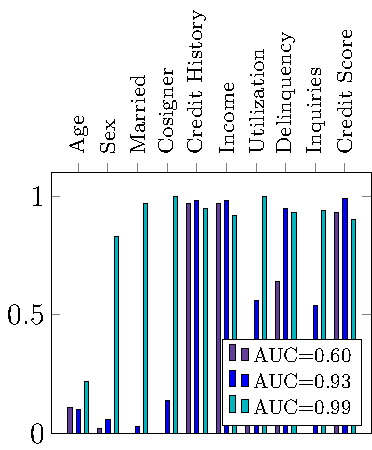
\includegraphics[width=.28\textwidth]{Figs/sec4_4_mlp_auc_shap-figure0.pdf}}%
                \label{subfig:mlp_avg_shap_sign_accs}%
            }\hspace{1cm}
            \subfloat[SHAP Concordance]{%
                 \raisebox{.05cm}{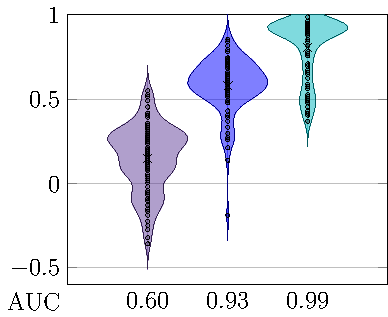
\includegraphics[width=.28\textwidth]{Figs/sec4_4_mlp_auc_shap-figure1.pdf}}%
                \label{subfig:mlp_auc_shap_spearmans}%
            }\hspace{1cm}
            \subfloat[SHAP Relevance]{%
                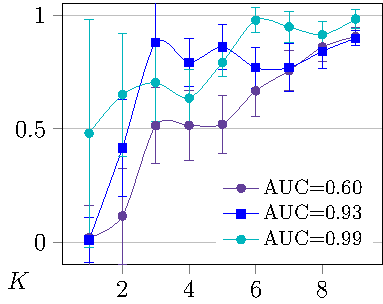
\includegraphics[width=.28\textwidth]{Figs/sec4_4_mlp_auc_shap-figure2.pdf}%
                \label{subfig:mlp_auc_shap_recalls}%
            }\\
            \subfloat[LIME Directionality]{%
                \raisebox{.2cm}{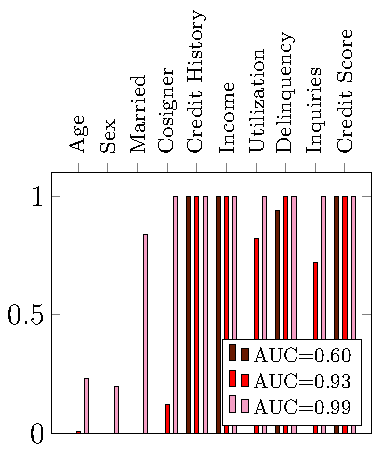
\includegraphics[width=.28\textwidth]{Figs/sec4_4_mlp_auc_lime-figure0.pdf}}%
                \label{subfig:mlp_auc_lime_sign_accs}%
            }\hspace{1cm}%\hfill
            \subfloat[LIME Concordance]{%
                \raisebox{.05cm}{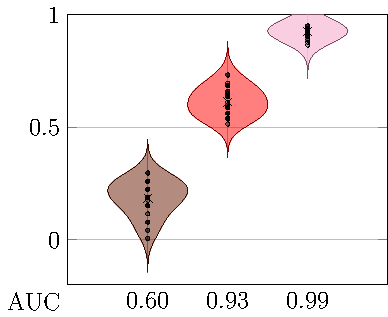
\includegraphics[width=.28\textwidth]{Figs/sec4_4_mlp_auc_lime-figure1.pdf}}%
                \label{subfig:mlp_auc_lime_spearmans}%
            }\hspace{1cm}
            \subfloat[LIME Relevance]{%
                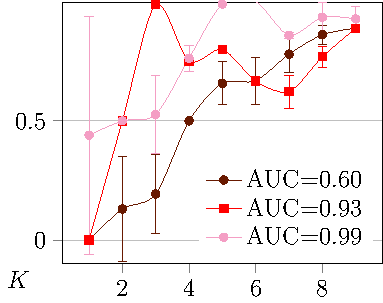
\includegraphics[width=.28\textwidth]{Figs/sec4_4_mlp_auc_lime-figure2.pdf}%
                \label{subfig:mlp_auc_lime_recalls}%
            }\\
            \caption{Comparisons of results for our three metrics for SHAP and LIME when explaining $\mathcal{M}_1$ with AUC=.6, $\mathcal{M}_2$ with AUC=0.92, and $\mathcal{M}_3$ with AUC=.99}
            \label{fig:mlp_auc_increase}
        \end{figure}

    
    %https://stats.stackexchange.com/questions/15011/generate-a-random-variable-with-a-defined-correlation-to-an-existing-variables
    \subsubsection{Role of Feature Independence}
        \label{sec:role_of_correlation}
The machine learning model $\mathcal{M}$ is developed through training on dataset $\mathcal{D}$, aiming to optimize then predictive performance. 
Then $\mathcal{M}$ establishes a mapping from inputs to outputs. However, this outcome-based optimization ensures only the accuracy of the predictions without controlling whether the mapping accurately reflects the true relationships in the data. In other words, it does not govern \emph{how} predictions are produced.

In real-world scenarios, features are typically interdependent. Thus, while the ideal model might rely predominantly on a specific set of features to determine the correct label, 
$\mathcal{M}$ might infer using a different, albeit similar, set of features. Consequently, 
$\mathcal{M}$ can arrive at the same predictions through an alternate mapping.
Complicating this issue is the fact that, regardless of opinions on the significance of dependent variables, machine learning models tend to overvalue features that provide information about multiple other features, as these are strong predictors of the target. Post hoc explainers then interpret the importance of such features in various ways, further muddying the understanding of feature relevance within an ML model.

Given that a feature's dependence on other features can skew its perceived importance in a model, and this importance may be estimated by an explainer to infer information about marginal effects, it is crucial to investigate whether there is a discrepancy between the importance of dependent features as assessed by a post hoc explainer and their significance as represented by their marginal effects. To demonstrate how dependent features can impact data-alignment, we will generate a modified version of the dataset from Section \ref{sec:data_generation} with mutually independent features. In this revised dataset, the credit score is independent of other features, such as credit utilization, credit inquiries, delinquencies, and credit history, rather than being derived from them. Additionally, the cosigner feature is now modeled as a Bernoulli-distributed random variable, independent of marital status. In this case, the marginal effects $\boldsymbol{\beta}$ of $\mathcal{G}$ match the coefficients from Equation \ref{eqn:gt}. %We normalize the SHAP values in an effort to show how feature independence can affect explanations obtained from SHAP, in spite of its inherent data-misalignment.


        Our experiment showed that by making credit score and cosigner independent, data-alignment increased overall and with respect to credit score and cosigner in particular. Figures \ref{fig:shap_corr_accs} and \ref{fig:lime_corr_accs} show that both SHAP and LIME's directionality for the cosigner feature improved by making it independent of marital status. SHAP's directionality for credit score also improved substantially. Our most striking results come from the massive increases in relevance and concordance, especially for LIME. Figure \ref{fig:lime_corr_recalls} shows that LIME was adept at identifying the top $k=1,2,3$ most important features when the features were independent while it could rarely (or never) do so when the features were not independent. Its mean concordance was also larger by about .2. SHAP saw significant gains in relevance for $k=1,\ldots,5$ (see  Figure \ref{fig:shap_corr_recalls})as well as small increase in concordance.
        \begin{figure}[h]
            \subfloat[SHAP Directionality]{%
                \raisebox{.2cm}{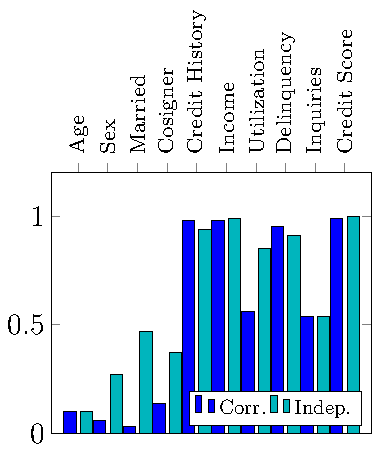
\includegraphics[width=.28\textwidth]{Figs/sec4_3_corr-figure1.pdf}}%
                \label{fig:shap_corr_accs}%
            }\hspace{1cm}%\hfill
            \subfloat[SHAP Concordance]{%
                \raisebox{.05cm}{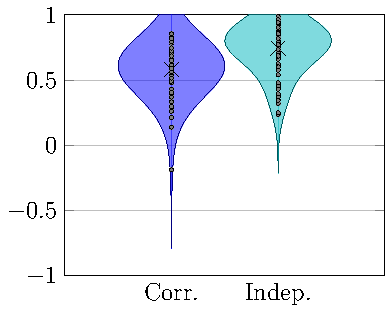
\includegraphics[width=.28\textwidth]{Figs/sec4_3_corr-figure3.pdf}}%
                \label{fig:shap_corr_spearmans}%
            }\hspace{1cm}%\hfill
            \subfloat[SHAP Relevance]{%
                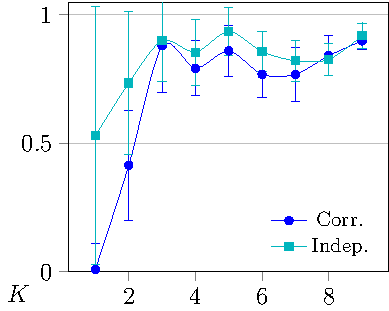
\includegraphics[width=.28\textwidth]{Figs/sec4_3_corr-figure5.pdf}%
                \label{fig:shap_corr_recalls}%
            }\\
            \subfloat[LIME Directionality]{%
                \raisebox{.2cm}{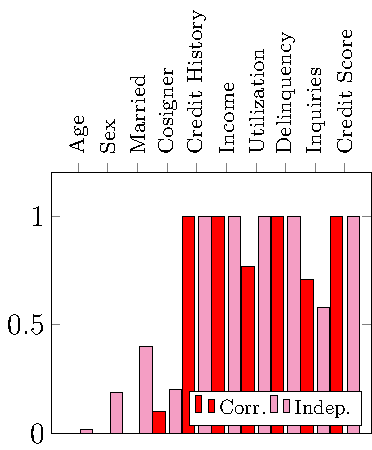
\includegraphics[width=.28\textwidth]{Figs/sec4_3_corr-figure0.pdf}}%
                \label{fig:lime_corr_accs}%
            }\hspace{1cm}%\hfill
            \subfloat[LIME Concordance]{%
                \raisebox{.05cm}{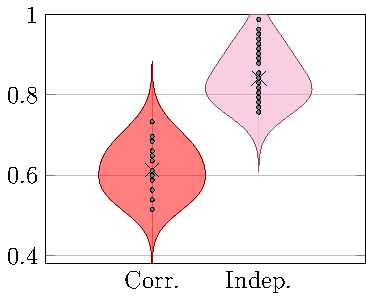
\includegraphics[width=.28\textwidth]{Figs/sec4_3_corr-figure2.pdf}}%
                \label{fig:lime_corr_spearmans}%
            }\hspace{1cm}%\hfill
            \subfloat[LIME Relevance]{%
                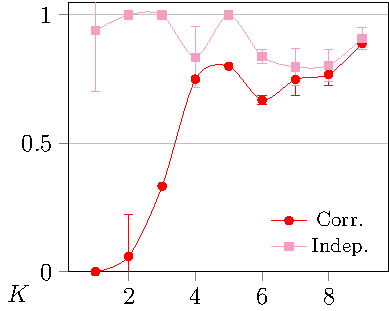
\includegraphics[width=.28\textwidth]{Figs/sec4_3_corr-figure4.pdf}%
                \label{fig:lime_corr_recalls}%
            }\\
            \caption{Comparison of faithfulness of explanations of models trained on data with independent features versus data with two strongly correlated features.}
            \label{fig:lime_shap_colinear}
        \end{figure}
    
    
    
    
    
    
\subsection{Pervasiveness of Data-Misalignment - a Large Scale Evaluation}
    \label{sec:pervasive}
    We used one simulated dataset to demonstrate the mis-alignment of the SHAP and LIME explanations. To study how pervasive the issue is, % We show that data-misalignment is a general property of SHAP and LIME. In doing this, the implications of Section \ref{sec:causes_of_misalignment} are corroborated and the scope of their validity is widened. We do this by evaluating the data-alignment of 
    We evaluate the SHAP and LIME explanations using 100 simulated datasets. To do that, we randomly generate binary classification datasets with between 3 and 100 i.i.d normally distributed features and between 100 and 10000 rows.  The targets of the datasets are initially produced using randomly generated linear decision boundaries, but are then corrupted with varying amounts of noise. We generate a model for each dataset using the Python AutoML package auto-sklearn. Their test set accuracies are between $.82$ and $.99$. It is important to note that as the features are normally distributed and mutually independent, this scenario is practically ideal.  
    %%We do not allow the AutoML to perform feature pre-processing. We set the AutoML to search among the following model types: MLP, XGBoost, Decision Tree, ExtraTrees, Random Forest, and \textcolor{red}{\ldots}. The models are evaluated using 5-fold cross validation with respect to test set accuracy. We run the AutoML in a parellelized fashion with 16 cores and allow a maximum of 10 minutes to produce a model for each dataset. 

    Since the number of features differs across the datasets, we report the results for our three metrics in the following fashion, conditioned on the number of features $d$. For each dataset with $d$ features, we compute the feature-wise mean directionality over $m=100$ test set instances and report the average over the datasets. Similarly, we report the mean and standard deviation of concordance, and mean relevance for $k=3$. 




    
    Our experimental results imply that SHAP and LIME explanations are generally not informative about marginal effects for datasets with more than thirty features. Indeed, Figure \ref{fig:lime_shap_vary_d} shows that, generally when $d$ exceeds $30$, mean directionality for SHAP and LIME is actually under $.5$, worse than random guessing. This is an alarming sign because the two most popular post hoc explainers can not even get the correct qualitative estimation of the true marginal effect - even the sign is wrong! In addition, both the mean concordance and mean relevance for $k=3$ are near $0$. It should be noted that the more features there are, the more challenging it is for the two explainers to correctly identify the contributions of each feature, as there exist more possible mappings from the input to the output that could be different from that of $\mG$ and there is no control over which one $\mM$ uses.

    
    \subsection{Discussion}
            Since researchers cannot directly access the ground truth model $\mathcal{G}$ and can only interact with an intermediary machine learning model $\mathcal{M}$, the process of explanation is bifurcated into two distinct stages: the prediction stage and the explanation stage. To generate explanations that accurately reflect the marginal effects, one must navigate challenges that may arise in either stage, necessitating additional assumptions about the data, $\mathcal{M}$, and the explanation tool $\mathcal{E}$. Crucially, $\mathcal{E}$ must possess the ability to accurately capture information regarding the marginal effectsThe discussion in Section \ref{sec:theoretical_considerations} describes theoretically why it is challenging for SHAP and LIME to draw even qualitative information (e.g. the sign) of the true marginal effect. If we presume $\mathcal{E}$'s competence in recovering the actual marginal effects, it becomes essential for $\mathcal{M}$ to closely approximate $\mathcal{G}$, ensuring that information about the marginal effects is indeed present within $\mathcal{M}$. Insights from Section \ref{sec:causes_of_misalignment} indicate that $\mathcal{M}$'s ability to achieve high predictive accuracy, especially when trained on data featuring mutually independent variables, significantly facilitates the extraction of the marginal effects.       \textbf{SHAP and LIME being data-misaligned appears to be a general phenomenon}, which worsens with \textit{low predictive performance of the machine learning model, dependence of features, and the large number of features}. 

      \begin{figure}[ht!]
      \captionsetup{labelfont=footnotesize,textfont=footnotesize}
      \captionsetup[subfloat]{labelfont=scriptsize,textfont=scriptsize,justification=centering}
      \centering
      \subfloat[SHAP Mean Directionality]{%
        \hspace{0mm}
        \raisebox{0cm}{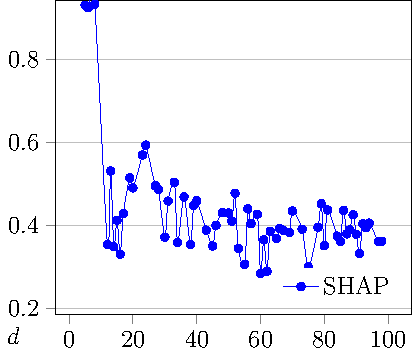
\includegraphics[width=0.178125\textwidth]{SynthFigs/meanaccshap-figure0.pdf}\quad}%
        \label{fig:shap_vary_d_spearmans}%
      }\hspace{1cm}%\hfill
      \subfloat[SHAP Concordance]{%
        \raisebox{0cm}{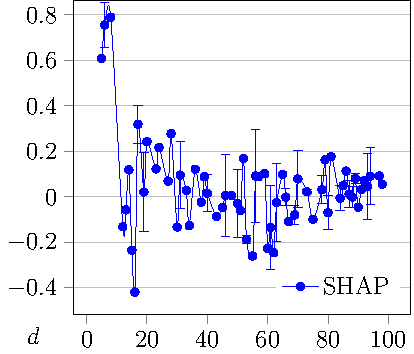
\includegraphics[width=0.178125\textwidth]{SynthFigs/concshap-figure0.pdf}}%
        \label{fig:shap_vary_d_accs}%
      }\hspace{1cm}%\hfill
      \subfloat[SHAP Top-3 Relevance]{%
        \raisebox{0cm}{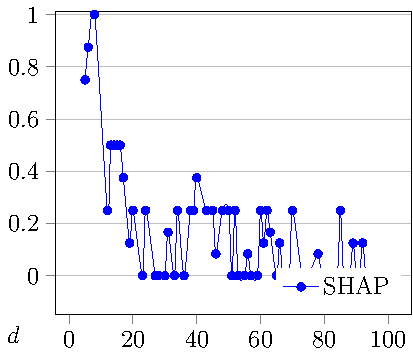
\includegraphics[width=0.178125\textwidth]{SynthFigs/relshap-figure0.pdf}}%
        \label{fig:shap_vary_d_spearmans}%
      }\\
      % \subfloat[LIME Top-1 Directionality]{%
      %   \raisebox{0cm}{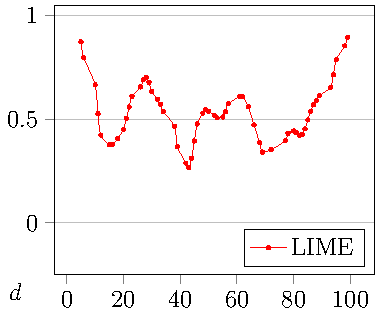
\includegraphics[width=.2\textwidth]{Figs/synthetic-figure1.pdf}}%
      %   \label{fig:lime_vary_d_accs}%
      % }\hspace{.5cm}%\hfill
      \subfloat[LIME Mean Directionality]{%
        \hspace{0mm}
        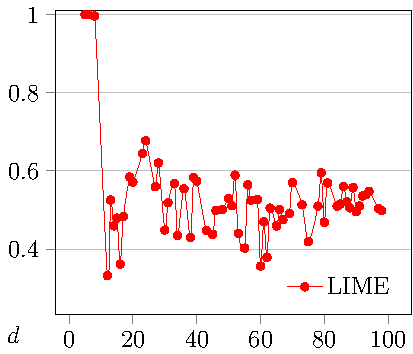
\includegraphics[width=0.178125\textwidth]{SynthFigs/meanacclime-figure0.pdf}\quad%
        \label{fig:lime_vary_d_spearmans}%
      }\hspace{1cm}%\hfill
      \subfloat[LIME Concordance]{%
        \hspace{0mm}
        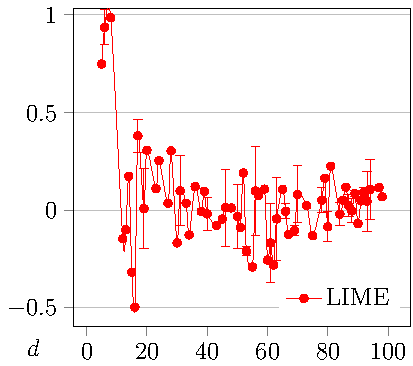
\includegraphics[width=0.178125\textwidth]{SynthFigs/conclime-figure0.pdf}%
        \label{fig:lime_vary_d_accs}%
      }\hspace{1cm}%\hfill
      \subfloat[LIME Top-3 Relevance]{%
        \hspace{0mm}
        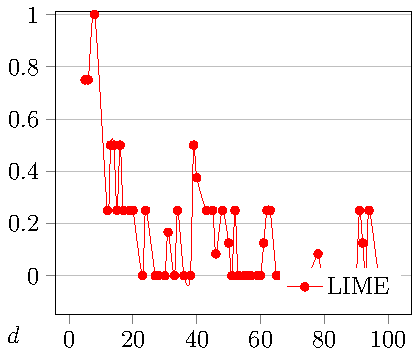
\includegraphics[width=0.178125\textwidth]{SynthFigs/rellime-figure0.pdf}%
        \label{fig:lime_vary_d_spearmans}%
      }\\
      \caption{Relationship of number of features $d$ with feature-wise mean directionality, concordance, and relevance for $k=3$}
      \label{fig:lime_shap_vary_d}
    \end{figure}


      \begin{figure}[ht!]
      \captionsetup{labelfont=footnotesize,textfont=footnotesize}
      \captionsetup[subfloat]{labelfont=scriptsize,textfont=scriptsize,justification=centering}
      \centering
      \subfloat[SHAP Mean Directionality]{%
        \hspace{0mm}
        \raisebox{0cm}{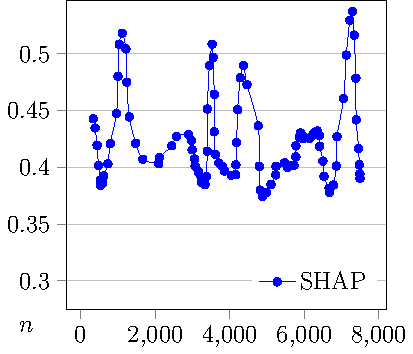
\includegraphics[width=0.178125\textwidth]{SynthFigs/meanaccshap_n-figure0.pdf}\quad}%
        \label{fig:shap_vary_n_spearmans}%
      }\hspace{1cm}%\hfill
      \subfloat[SHAP Concordance]{%
        \raisebox{0cm}{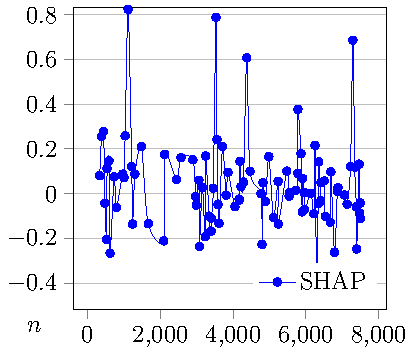
\includegraphics[width=0.178125\textwidth]{SynthFigs/concshap_n-figure0.pdf}}%
        \label{fig:shap_vary_n_accs}%
      }\hspace{1cm}%\hfill
      \subfloat[SHAP Top-3 Relevance]{%
        \raisebox{0cm}{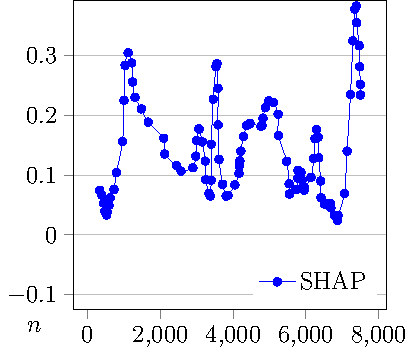
\includegraphics[width=0.178125\textwidth]{SynthFigs/relshap_n-figure0.pdf}}%
        \label{fig:shap_vary_n_spearmans}%
      }\\
      % \subfloat[LIME Top-1 Directionality]{%
      %   \raisebox{0cm}{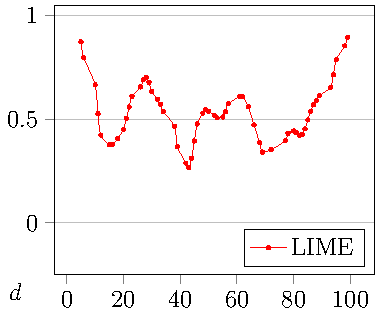
\includegraphics[width=.2\textwidth]{Figs/synthetic-figure1.pdf}}%
      %   \label{fig:lime_vary_d_accs}%
      % }\hspace{.5cm}%\hfill
      \subfloat[LIME Mean Directionality]{%
        \hspace{0mm}
        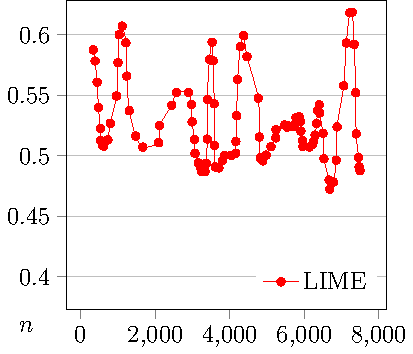
\includegraphics[width=0.178125\textwidth]{SynthFigs/meanacclime_n-figure0.pdf}\quad%
        \label{fig:lime_vary_n_spearmans}%
      }\hspace{1cm}%\hfill
      \subfloat[LIME Concordance]{%
        \hspace{0mm}
        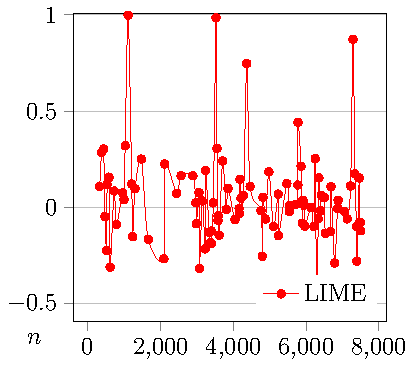
\includegraphics[width=0.178125\textwidth]{SynthFigs/conclime_n-figure0.pdf}%
        \label{fig:lime_vary_n_accs}%
      }\hspace{1cm}%\hfill
      \subfloat[LIME Top-3 Relevance]{%
        \hspace{0mm}
        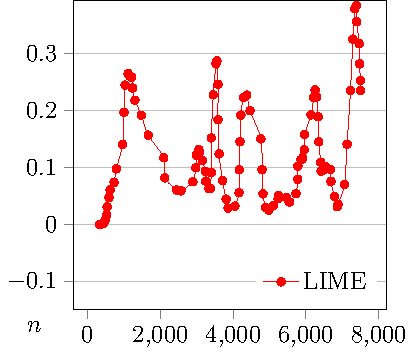
\includegraphics[width=0.178125\textwidth]{SynthFigs/rellime_n-figure0.pdf}%
        \label{fig:lime_vary_n_spearmans}%
      }\\
      \caption{Relationship of number of features $n$ with feature-wise mean directionality, concordance, and relevance for $k=3$}
      \label{fig:lime_shap_vary_n}
    \end{figure}






%The contributions of the confounding and confounded features are concealed unless one has knowledge of the true causal graph underlying the dataset. The faithfulness of explainers of models trained on such data is also harmed. 
           %Because a dataset affected by an unobserved confounder lacks crucial information about the ground truth, explanations of models trained on such datasets naturally must be unfaithful to the ground truth. 

            %The necessity of causal inference conditions is especially important for business research because faithful and interesting business insights are preferably causal relations. Being able to gather, say, that there is a correlation between age and loan approval likelihood without having access to the ground truth is no doubt valuable, but it would be indisputably better if the relationship can be concluded to be causal.

% Change from CIST version: Rashomon -> inconsistency
% https://stackoverflow.com/questions/75638742/why-shap-values-are-the-same-every-time-if-kernel-shap-is-based-on-random-sampl
% SHAP is (nearly) deterministic



% \section{Inconsistency of Post Hoc Explanations}
%     \label{sec:inconsistency}
%     Another major issue post hoc explanations  suffer from is inconsistency, which refers to one or more post hoc explainers providing conflicting information about the marginal effects. Inconsistency is a source of confusion and frustration because without sufficient domain knowledge, misaligned explanations cannot be distinguished from aligned ones. Inconsistency can facilitate generation of invalid hypotheses and invalid inference because users without domain knowledge that are not able to account for inconsistency may be forced to make arbitrary selections of explanations. 

%     Explanation inconsistency has to do with the \textit{model being explained} (i.e., $\mathcal{M}$) and the \textit{explainers} (i.e., $\mathcal{E})$. Fixing one explainer and varying $\mathcal{M}$  may yield differing hypotheses about the marginal effects. This variation is due to the different ways in which models capture and approximate the ground truth ($\mathcal{G}$) and their unique decision-making processes, which can significantly diverge even when their predictions appear similar. Factors such as the dataset characteristics and the internal mechanisms and structures of $\mathcal{M}$ influence these outcomes. Conversely, for a fixed $\mathcal{M}$, explanations could still vary due to inherent differences among the explainers or differing configurations of an explainer's hyperparameters. We provide in Appendix Section \ref{sec:appendix_inconsistency} a set of experiments that demonstrate how inconsistency arises with different combinations of explanation methods and models. For example, we show that both the feature rankings and signs from pairs of SHAP and LIME explanations of the same prediction are usually different.

%     In Appendix Section \ref{sec:instability} we also explore a more general form of inconsistency known as instability. Inconsistency of explanations for similar inputs is called instability. Instability can manifest when, e.g., two applicants with similar profiles get different explanations and can lead to uncertainty about which explanation better represents the marginal effects and possibly unfounded suspicions that the decision process is unfair. 


          
%           %At any rate, the issue of inconsistency makes it difficult to justify any one explanation or pipeline configuration if one does not have sufficient domain knowledge, since alternatives abound with equal plausibility. It follows that researchers who wish to use SHAP or LIME to generate hypotheses about their data should take care in doing so. Researchers should be reticent if considering proclaiming that they have identified some novel phenomena via post hoc feature importance values since such novelty could merely be an artifact of inconsistency. Inconsistency thus facilitates generation of invalid hypotheses and invalid inference because users without domain knowledge that are not able to account for inconsistency are forced to make arbitrary selections of explanations. %We also discussed how the volatility of the decision boundary of $\mathcal{M}$ in comparison to the volatility of the decision boundary of $\mathcal{G}$ affects explanation stability. Explaining an underfit $\mathcal{M}$ as part of a fairness audit of $\mathcal{G}$ could cause unfairness to go unnoticed. Conversely, explanations of similar inputs to an overfit $\mathcal{M}$ could be dissimilar and cause confusion and make neither explanation justifiable. %Consider, for example, how Figure \ref{fig:lime_rankings_mag} shows that LIME may indicate that the least important feature is the most important (and vice versa).
         



\section{Mitigation Strategies}
    \label{sec:mitigation_strategies}
    In this section, we use the results of our experiments and the implications of the theoretical results from Section \ref{sec:theoretical_considerations} to propose and test some simple mitigation strategies for misalignment and inconsistency. The strategies we propose here are meant to be sufficiently simple to understand and use such that they form a platform for further exploration and experimentation. We soften the impact of our choices for data and model in this section by using the version of our dataset with mutually independent features and an MLP with accuracy and test set ROC AUC equal to $.99$ in each experiment unless otherwise stated. To begin the section, we will introduce the criteria we use to test if a strategy improves data-alignment over a baseline with respect to directionality, concordance, and relevance. Then we describe and demonstrate our mitigation strategies, starting with those that are specific to SHAP or LIME and concluding with generally applicable strategies. Using our definitions of improvement, the mitigation strategies we propose are all effective in at least one respect. We provide results for less effective mitigation strategies in Appendix Section \ref{sec:appendix_mitigations}. 

    %\subsection{Mitigation Strategies for misalignment}
    %\label{sec:incorrectness_mitigation} %\textcolor{red}{move this to the end of section 4. this is the mitigation strategy for incorrectness}
    
        %We propose a few intuitive mitigation strategies for explanation faithfulness based on data pre-processing and, model training, and explainer hyperparameters. We first demonstrate the truth of Corrolaries 1 and 2 from Section \ref{sec:theoretical_considerations}. We then verify that ensuring both that $\mathcal{M}$ has high test set accuracy and that its training data has no unobserved, correlated, or confounded features is associated with increased explanation quality. The next strategy involves ensuring that $\mathcal{M}$ has high test set ROC AUC. The final strategy involves ensuring that the underlying model of $\mathcal{E}$ correctly classifies the input being explained. When demonstrating the first, third, and fourth strategies, the training data do not have unobserved, correlated, or confounded features in order to isolate the roles of $\mathcal{E}$ and $\mathcal{M}$. 
    \subsection{Testing Improvement}
        \label{sec:improvement}
        This section introduces the hypothesis testing framework that we use to characterize whether an explanation method $\mE^\prime$ improves over a baseline explanation $\mE$ in terms of directionality, concordance, relevance, and consistency. All details, including statements of the null and alternative hypotheses we use, can be found in Appendix Section \ref{sec:hypothesis_testing}.
        
        
        The underlying idea for our tests for improvement of directionality, concordance, relevance, and consistency of rankings, is to test if the mean(s) of the parameter(s) of interest is(are) higher for $\mE^\prime$ than for $\mE$ using Wilcoxon signed-rank tests on the location of mean of differences from a matched sample(s). When testing for improvement of consistency of feature importance signs, we use one-sided McNemar tests for whether pairs of the pipeline with the mitigation strategy applied and baseline disagree on feature importance signs at the same rate. All of our tests are performed with a significance level of $\alpha=.05$. 
        
        We utilize a rather strict characterization of improvement for data-alignment. Our tests are meant to capture when $\mE^\prime$ has a significant improvement over $\mE$ in at least one respect and is not significantly worse than $\mE$ in any respect. For example, we would not say that $\mE^\prime$ improved directionality overall if $\mE$ had better directionality for a single feature while $\mE^\prime$ had better directionality for all other features. 
        
        
     


    \subsection{Explainer Specific Strategies}
        Before discussing general-use strategies, we will present three strategies applicable only to SHAP or LIME (but not both). All strategies involving SHAP will make use of the simple normalization scheme outlined in Section \ref{sec:theoretical_considerations} as otherwise the strategies would not appear to do anything.


            \subsubsection{Normalizing The Shapley Value}
                It follows directly from the theory underlying SHAP that SHAP values do not represent $\boldsymbol{\beta}$, and so it is therefore worthwhile to seek practical ways to modify our usage of SHAP. Since equation \ref{eqn:shap_gt} showed that SHAP returns $e_{\text{SHAP}}(\mathbf{x}^{(i)})=\boldsymbol{\beta}^T(\mathbf{x}^{(i)} - \bar{\mathbf{x}})$ instead of $\boldsymbol{\beta}$, we proposed in Section \ref{sec:theoretical_considerations} to instead take the importance of feature $j$ to be $e_{\text{SHAP}}(x^{(i)}_j) / (x^{(i)}_j - \bar{x}_j)$ where $\bar{x}_j$ is the empirical mean of feature $j$ from the training data because this expression should be approximately $\beta_j$. Our experiments confirmed the advantage of this technique; Figure \ref{fig:shap_dividex_corr} showed that unmodified SHAP explanations perform about as well as random ones with respect to our three metrics while the normalized SHAP explanations performed quite well with respect to our three metrics. In addition, the normalized SHAP explanations were more consistent across individuals (recall that Figure \ref{fig:shap_dividex_spearmans} showed that the concordance distribution for normalized SHAP explanations had a significantly smaller region of support which, importantly, was centered at a larger value than the mean concordance of the unmodified SHAP explanations). Since these results were produced using the version of our dataset with correlated features, we additionally provide a comparison of SHAP without and with normalization when the input features are independent in Appendix Section \ref{sec:shap_norm_indep}.



        
        \subsubsection{Increasing $\nu$ and $n$ for LIME } 
            \label{sec:lime_params}
            Corollaries 1 and 2 from Section \ref{sec:theoretical_considerations} imply that LIME's kernel bandwidth $\nu$ and number of perturbed samples $n$ need to be large in order for $e_{\text{LIME}}(x_j)$ to be close to $\boldsymbol{\beta}$, so this section will experiment with how their respective sizes affect explanation quality. In our experiment, we compare the concordance of $m=100$ explanations by LIME surrogate models using the default $\nu = .75\sqrt{d}$ (where $d$ is the number of features) and $n=1000$ with LIME surrogate models using $\nu=n=10000$. 
            
            We found that increasing the number of samples $n$ and the kernel bandwith $\nu$ improves directionality, concordance, and relevance. Our results are shown in Figure \ref{fig:lime_tuning}. Although the results for ``credit history", ``credit score", ``delinquency", ``income", ``inquiries", and ``utilization" were identical before and after the strategy was applied, we found that increasing $\nu$ and $n$ directionality improved significantly for the remaining features, as our Wilcoxon tests for equal signs accuracies had p-values of $0.01$ for ``age", $2.34e-3$ for ``cosigner", and $1.65e-9$ for ``sex". The larger $\nu$ and $n$ also resulted in pairs of rankings whose concordances were both larger on average; the p-value for our test for equally consistent rankings was $1.97e-14$. %The plot of $\text{relevance}_k$ shows that using $\nu=n=10000$ netted a strict advantage for correctly ranking the features which were not the most or least important. That is, for $k=1$ the results were identical and for $k=2,8$ we fail to reject the null hypothesis of equal relevances with a p-values of $0.08$ and $0.12$ respectively, but we do reject the null hypotheses for $k=3,\ldots,7$ with p-values of $9.14e-5$, $4.56e-4$, $1.71e-7$, $2.64e-11$, and $5.90e-12$.
        
            \begin{figure}[ht!]
                \centering
                \begin{subfigure}[t]{.28\textwidth}
                  \centering
                  \captionsetup{justification=centering}
                      \raisebox{.2cm}{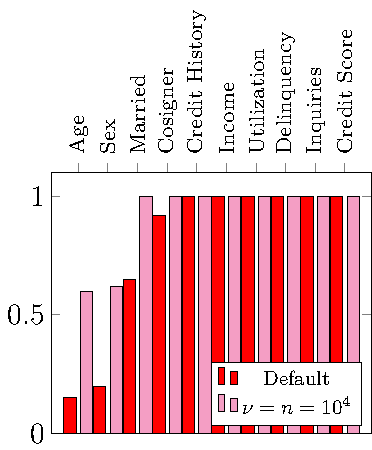
\includegraphics[width=\textwidth]{Figs/fig4_4_LIME-figure0.pdf}}%{Figures/lime_shap_Spearman_magnitude.png}
    
                  \caption{Directionality}%Spearman rank correlations of feature importance magnitudes from SHAP and LIME against the true ranking from $\mathcal{G}$. }
                   \label{fig:lime_tuning_sign_accs}
                \end{subfigure}%
                \hspace{1cm}
                \begin{subfigure}[t]{.28\textwidth}
                  \centering
                   \captionsetup{justification=centering}
                  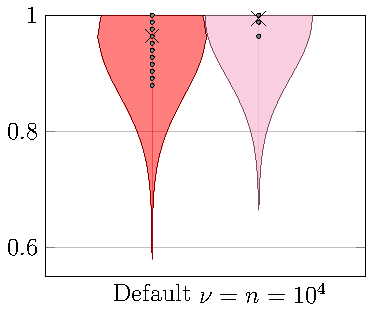
\includegraphics[width=\textwidth]{Figs/fig4_4_LIME-figure1.pdf}%{Figures/lime_shap_Spearman_signed.png}
                  \caption{Concordance}%Spearman rank correlations of signed feature importance from SHAP and LIME against the true ranking from $\mathcal{G}$.}
                   \label{fig:lime_tuning_spearmans}
                \end{subfigure}
                \hspace{1cm}
                \begin{subfigure}[t]{.28\textwidth}
                  \centering
                   \captionsetup{justification=centering}
                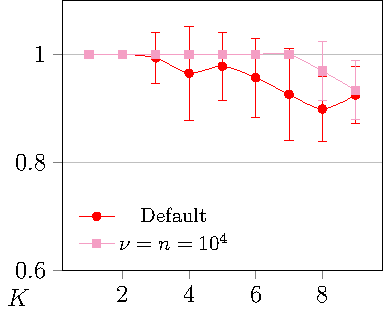
\includegraphics[width=\textwidth]{Figs/fig4_4_LIME-figure2.pdf}%
                \caption{Relevance}%The average and standard error of recall of SHAP and LIME when attempting to capture the top K most important features to $\mathcal{G}$ when explaining $\mathcal{M}$, for varied $K=1,2,3,...$ number of features.}
                \label{fig:lime_tuning_recalls}
                \end{subfigure}
                \caption{Comparison of LIME explainer with default settings versus $\nu=n=10000$ with respect to our three metrics}
               \label{fig:lime_tuning}
            \end{figure} 

            \subsubsection{Averaging Explanations of One Model by Different Explainers}
            \label{sec:averaging_one_explainer}
            Although the inconsistency of the explanations described in Section \ref{sec:conflict_between_within} is unfortunate because it makes individual explanations seem less plausible, we wondered if it could actually be leveraged into an advantage. Each explanation likely has at least a modicum of truth, and so we seek an aggregation strategy that increases the signal to noise ratio. To this end, we investigate whether there is a tendency for an explanation constructed using the average feature importance values over a set of LIME explainers with different hyperparameters to be superior to single explanations from LIME with its default settings. We do not test this strategy with SHAP since its explanations at the individual level are deterministic. 
            
            Additional experiments using different explanation aggregation methods are provided in the Appendix. In particular, we demonstrate that combining one LIME and one (unmodified) SHAP explanation of the same prediction gives a worse explanation than either of the individual explanations. This is because SHAP and LIME have different underlying meanings of feature importance; combining them is not constructive because they have different goals. 
        
            We test if averaging explanations from LIME explainers aids data-alignment by comparing the explanations of the prediction of an MLP on $m=100$ applications by one LIME with the average explanation of 100 LIMEs. The 100 LIME explainers are created using random seeds $1,\ldots,100$ and default settings. The averaged explanation for each applicant is constructed by averaging over the feature importance values from the 100 LIME explanations of the applicant.  %We repeat this with $\nu=n=10000$. 

            Our statistical tests of improvement concluded that directionality, concordance, and relevance were significantly improved by using averaged instead of single LIME explanations. Averaging LIME explanations resulted in an enhanced ability to find the sign of several features (see Figure \ref{fig:lime_avg_sign_accs}). The mitigation did not change the assignment of signs for ``credit history", ``credit score", ``delinquency", ``income", ``inquiries", and ``utilization", but we were able to reject the null hypothesis of equal sign accuracies for ``age", ``cosigner", ``married", and ``sex" all with with $p<.001$. %$3.32e-3$, $2.34e-3$, $3.17e-5$, and $2.12e-6$, respectively.
            Moreover, the rankings produced by the averaged explanations were more concordant with the ground truth; we rejected the null hypothesis of equal concordances with a p-value of $7.39e-12$. %Figure \ref{fig:lime_avg_recalls} also shows that the averaged explanations were more likely to identify the features which were not the most or least important. 

            % \begin{table}[]
            % \centering
            % \begin{tabular}{|l|l|l|l|l|l|l|l|l|l|}
            % \hline
            % Age  & Cosigner & Credit History & Credit Score & Delinquency & Income & Inquiries & Married & Sex & Utilization \\ \hline
            % 0.98 & 1.20e-7   & n/a            & n/a          & n/a         & n/a    & 0.50      & 1.11e-4 & .12 & n/a         \\ \hline
            % \end{tabular}
            % \caption{p-values for improvement to consistency of feature importance signs by using averaged LIME explanations. Values are listed as ``n/a" if both pairs of explanations always found the correct sign for the corresponding feature.}
            % % \label{tab:lime_avg_sign_con}
            % \end{table}
                             
            \begin{figure}[!h]
            \centering
                \begin{subfigure}[t]{0.28\textwidth}
                \centering
                \raisebox{.2cm}{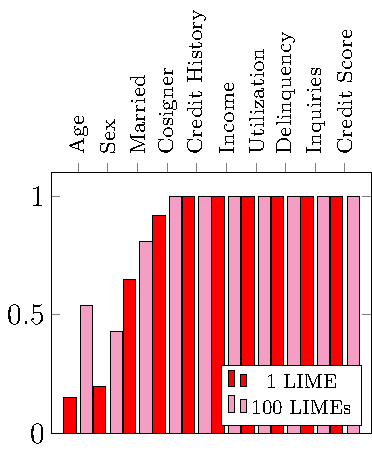
\includegraphics[width=\textwidth]{Figs/sec5_2_lime_avg2-figure0.pdf}}
                \caption{Directionality} \label{fig:lime_avg_sign_accs}
            \end{subfigure}\hspace{1cm}
            \begin{subfigure}[t]{0.28\textwidth}
                \centering
                \raisebox{.05cm}{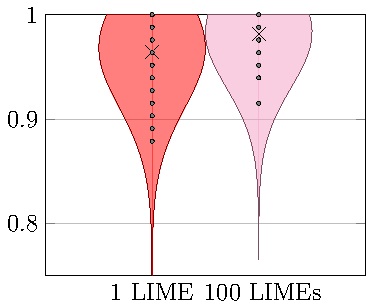
\includegraphics[width=\textwidth]{Figs/sec5_2_lime_avg2-figure1.pdf}}
                \caption{Concordance} \label{fig:lime_avg_spearmans}
            \end{subfigure}\hspace{1cm}
             \begin{subfigure}[t]{0.28\textwidth}
                \centering
                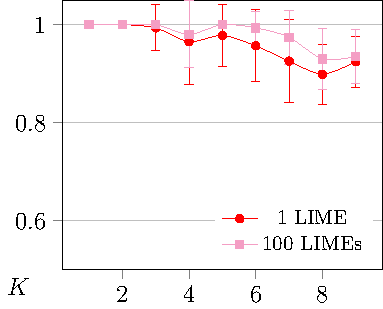
\includegraphics[width=\textwidth]{Figs/sec5_2_lime_avg2-figure2.pdf}
                \caption{Relevance}
                \label{fig:lime_avg_recalls}
            \end{subfigure}
            \caption{Comparisons of results for our three metrics for  explanations of an MLP $\mathcal{M}$ by 1 LIME explainer versus those created by averaging the feature importance values of 100 LIME explanations of $\mathcal{M}$}\label{fig:lime_avg}
            \end{figure}

                
            It was also the case that the averaging routine significantly improved consistency. To obtain this result, we created another set of average explanations from 100 more LIME explainers using random seeds $101,\ldots,200$, and tested whether the signs and rankings were more consistent between the two sets of averaged explanations compared to the signs and rankings of the two individual LIME explainers. We rejected the null hypotheses of our tests for equal consistency of feature importance signs in favor of improvement for ``age", ``cosigner", and ``married" all with $p<.001$.%of  $8.65e-3$, $1.20e-7$ and $1.11e-4$, respectively.
            There was no change for ``credit  history", ``credit score", ``delinquency", ``income", and ``utilization" because both methods were perfect in each case.  With a p-value of $7.60e-15$, we rejected the null hypothesis of our Wilcoxon test that the means of the two concordance distributions are equal in favor of the alternative hypothesis that the mean of the concordance distribution from the averaged explanations is larger. That this is the case is also visually evident from Figure \ref{fig:lime1_v_100_incon}; the concordance distribution of the averaged explanations was more concentrated near 1 and its tail was also shorter. 

            \begin{figure}[ht!]
                \centering
                %\begin{subfigure}{.3\textwidth}
                  \centering
                  \captionsetup{justification=centering}
                  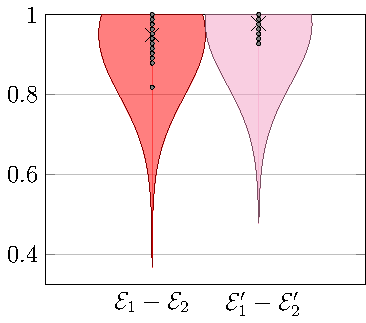
\includegraphics[width=.28\textwidth]{Figs/sec5_2_lime_avg2-figure3.pdf}
                  \caption{Comparison of concordances between explanations from pairs of individual LIME explainers and between pairs of averaged explanations from two sets of 100 LIME explainers.}%Spearman rank correlations of ranked feature importance magnitudes from LIME against the true ranked magnitudes from $\mathcal{G}$.}
                   %\label{fig:lime_income}
                %\end{subfigure}%
                %\caption{}%Violin plots of feature importance values for \emph{income} from SHAP and LIME for cases when \emph{income} is unconfounded and confounded by the unobserved social support feature}
                \label{fig:lime1_v_100_incon}
            \end{figure}
                
    \subsection{General Strategies}
        We now provide three general strategies to produce explanations that are more data-aligned. Recall that we have been using normalized Shapley values since otherwise the explanation are not better than random with respect to data-alignment. %To show the utility of these strategies for SHAP, we will use normalized SHAP values in each the experiments below. 

        \subsubsection{Optimizing the Tradeoff between Complexity and Predictive Power}
            \label{sec:decreasing_complexity}
            In view of the facts that 1) given some dataset many models $\mathcal{M}$ exist with approximately the same generalization error and 2) the complexity (number of parameters) of a model is a basic factor that distinguishes it, it makes sense to analyze what role the complexity of $\mathcal{M}$ plays on data-alignment. Since we established in \ref{sec:role_of_predictive_power} an association between the predictive performance of $\mathcal{M}$ and the faithfulness of LIME explanations of $\mathcal{M}$ with respect to $\mathcal{G}$, this mitigation strategy proposes to ensure that $\mathcal{M}$ has both good predictive performance and minimal complexity.\footnote{This strategy can be motivated by recalling the phenomenon in least squares polynomial regression that $r^2$ increases with the degree of the regressors regardless of how simple the mapping underlying the dataset is.} The labels predicted by $\mathcal{M}$ (after thresholding its output probabilities) agreeing with those in the test set is an incomplete representation of faithfulness to $\mathcal{G}$; even if $\mathcal{M}$ had 100\% training and testing accuracy on data with no measurement error this does not mean $\mathcal{M}=\mathcal{G}$. Thus, it is worth making an effort not to over-parameterize $\mathcal{M}$. To carry out this strategy, one can iteratively train and evaluate models of successively lower complexity and stop the procedure once the reduction of complexity leads to a substantial reduction in predictive performance. 
            
            To investigate this tradeoff as it pertains to data-alignment, we compare SHAP and LIME explanations of two MLPs (perceptrons, actually) of differing complexity but essentially the same predictive performance. The first MLP, $\mathcal{M}_1$, has 100 nodes in its hidden layer (the default in sklearn) and a test set AUC of about $.99$. The second, simpler MLP $\mathcal{M}_2$, has only two nodes in its hidden layer and yet also has a test set AUC of about $.98$. Figure \ref{fig:decreasing_complexity} visualizes our comparison of explanations of $\mathcal{M}_1$ and $\mathcal{M}_2$. Additional results and further motivation for this strategy can be found in Appendix Section \ref{sec:appendix_inconsistency}.

            We found that with the exception of relevance for SHAP, all three metrics were improved for both explainers. However, as shown by Figure \ref{fig:decreasing_complexity}, the improvements were marginal for the most part. For SHAP, we reject the null hypothesis of equal sign accuracies only for age with a p-value of $2.76e-9$ and credit history with a p-value of $0.04$. It is evident from Figure \ref{subfig:decreasing_complexity_shap_spearmans} that concordance did not rise significantly; we failed to reject the null hypothesis of equal concordances with a p-value of $.16$. Although relevance worsened for $k=8$ when explaining $\mathcal{M}_2$, the small improvements for $k=1,2,4,5,6,7$ were significant all with $p<.001$ except for $k=4$, which had $p=4.73e-2$.% $6.21e-3$, $9.83e-4$, $4.73e-2$, $7.85e-5$, $9.73e-6$, and $8.17e-17$.
            For LIME, we could only conclude that the directionality of ``married" improved by rejecting the null hypothesis of equal directionality with a p-value of $0.015$. However, the improvement to concordance was significant as its test had a p-value of $4.90e-5$. As for relevance, the results for $k=1$ were identical and the null hypothesis of equal relevance was rejected in favor of improvement for $k=2,6$ with p-values of $0.02$ and $0.01$. 
            
            A reason that the explanations of the simple model $\mathcal{M}_2$ were better is that even though $\mathcal{M}_1$ may have similar behavior in how they generate training and test set labels, the additional expressive power of $\mathcal{M}_1$ allows the local behavior of its decision boundary to be more erratic. Given that SHAP and LIME are local function approximators, incorrect local behavior of $\mathcal{M}_1$ imposes a limitation on how data-aligned SHAP and LIME can be when explaining $\mathcal{M}_1$. 

            
        \begin{figure}[t!]
            \subfloat[SHAP Directionality]{%
                \raisebox{.2cm}{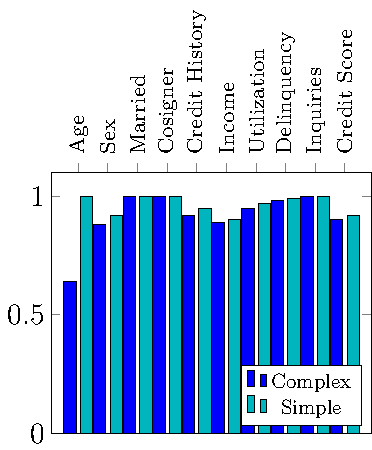
\includegraphics[width=.28\textwidth]{Figs/sec5_mlp_complexity-figure1.pdf}}%
                \label{subfig:decreasing_complexity_shap_sign_accs}%
            }\hspace{1cm}
            \subfloat[SHAP Concordance]{%
                \raisebox{.05cm}{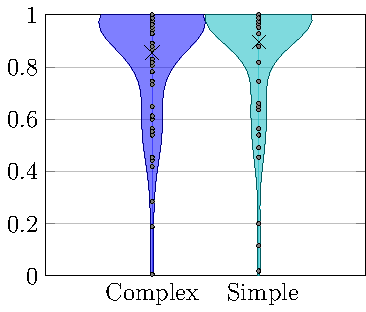
\includegraphics[width=.28\textwidth]{Figs/sec5_mlp_complexity-figure3.pdf}}%
                \label{subfig:decreasing_complexity_shap_spearmans}%
            }\hspace{1cm}
            \subfloat[SHAP Relevance]{%
                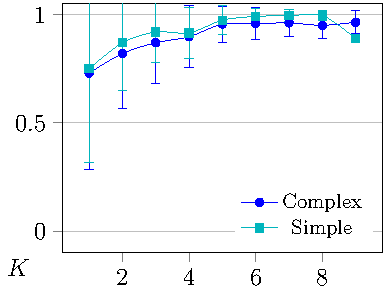
\includegraphics[width=.28\textwidth]{Figs/sec5_mlp_complexity-figure5.pdf}%
                \label{subfig:decreasing_complexity_shap_recalls}%
            }\\
            \subfloat[LIME Directionality]{%
                \raisebox{.2cm}{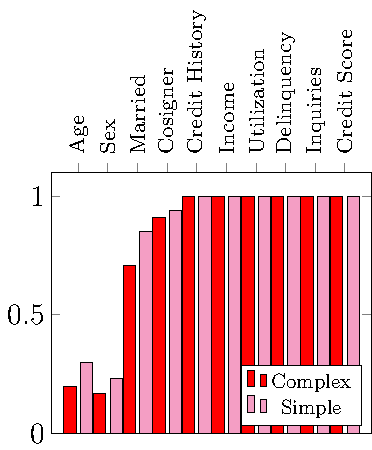
\includegraphics[width=.28\textwidth]{Figs/sec5_mlp_complexity-figure0.pdf}}%
                \label{subfig:decreasing_complexity_lime_sign_accs}%
            }\hspace{1cm}
            \subfloat[LIME Concordance]{%
                \raisebox{.05cm}{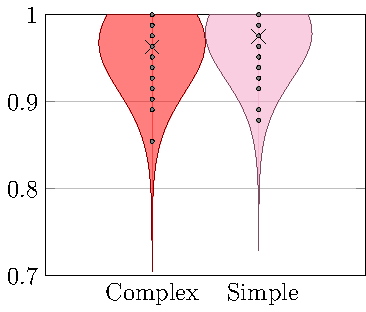
\includegraphics[width=.28\textwidth]{Figs/sec5_mlp_complexity-figure2.pdf}}%
                \label{subfig:decreasing_complexity_lime_spearmans}%
            }\hspace{1cm}
            \subfloat[LIME Relevance]{%
                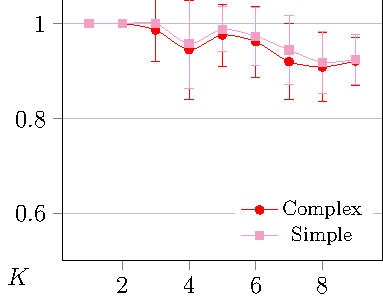
\includegraphics[width=.28\textwidth]{Figs/sec5_mlp_complexity-figure4.pdf}%
                \label{subfig:decreasing_complexity_lime_recalls}%
            }\\
            \caption{Comparisons of results for our three metrics for SHAP (top row) and LIME (bottom row) explanations of equally accurate MLPs with high and low complexity.}
            \label{fig:decreasing_complexity}
        \end{figure}

     %simple models used here
        %\subsubsection{Tuning $\mathcal{M}$ with Minimal Complexity}
        %    \label{sec:m_fidelity}


            %We then demonstrated in Section \ref{sec:role_of_causal}, keeping the predictive performance of $\mathcal{M}$ approximately constant, that (LIME) explanations of a model $\mathcal{M}$ were better equipped to recover $\boldsymbol{\beta}$ when $\mathcal{M}$ was trained on data without correlation or confounding. Whenever possible, it is therefore worthwhile to pre-process data in a way that accounts for correlated and confounded features. %We will show in Appendix Section \ref{sec:backdoor_adjustment} a way to do this that requires knowledge of the true structural causal model underlying the dataset. 

        %\subsubsection{Near Perfect Test Set Accuracy of Model Trained on Ideal Dataset}
            %\label{sec:optimal_conditions}
            %This mitigation strategy relies on the intuition that post hoc explanations should have the best results when the conditions for their use are practically ideal in the senses that 1) $\mathcal{M}$ has very high test set AUC and 2) the dataset satisfies the causal inference conditions. To satisfy the two aforementioned conditions, we again use the low-dimensional dataset with no causal inference violations from Section \ref{sec:causes_of_misalignment} but train $\mathcal{M}$ so that attains 99\% test set accuracy and an AUC of .98.
            
            %. Figure \ref{fig:lime_shap_g} shows that, when explaining $\mathcal{M}$, LIME is able to extract the true feature ranking and gets close with high consistency. SHAP usually does not recover the true feature Spearman Rank Correlations and additionally has more variance in the ranking distribution. %When explaining $\mathcal{G^*}$ itself, LIME seems to be able to perfectly recover the true ranking order almost always. When explaining $P_1$, SHAP can actually recover the true feature Spearman Rank correlations, but with less consistency than LIME does. 
        
            %We repeat the experiments of Section \ref{sec:evaluating_faithfulness} once more, but this time explain the aforementioned highly accurate model. Our results appear in Figures \ref{fig:perfect_data_model}. The main difference between we observed after raising the AUC of $\mathcal{M}$ from .95 to .99 occured with respect to the recall metric. Most notably, we can see from Figure \ref{fig:perfect_data_model_recalls} that LIME's average $\text{relevance}_k$ was equal to 1 for $k=1,2$ and closer to $1$ for $k=3,4$ than in Figure \ref{fig:avg_recall}. SHAP's $\text{relevance}_k$ also improved both in terms of mean and variance over the 100 applicants. However, there was not a signicant difference in the sign accuracy and rank correlation metrics.
            
            %Moreover, SHAP and LIME both still admit the possibility of misalignment in this scenario, despite the conditions for their use being in some sense ideal. For example Figure \ref{fig:perfect_data_model_acc} shows that SHAP and LIME could still only correctly identify how age impacts loan application likelihood for about half of the applicants.% in 
            
        % %use fbox to tailor crop
        % \begin{figure}[ht!]
        % \centering
        %     \begin{subfigure}{.3\textwidth}
        %     \centering
        %     %\fbox{\includegraphics[width=\textwidth,trim=0 10 70 70 mm, clip=true]{Figures/fig21.pdf}}%{Final_Figures/fig20.png}
        %     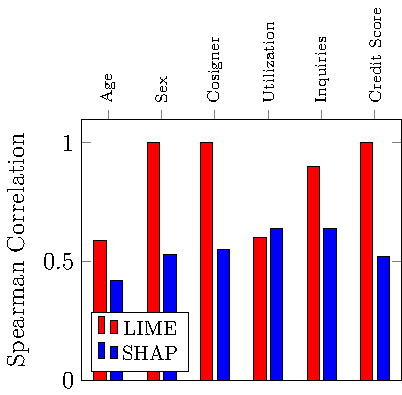
\includegraphics[width=\textwidth]{FinalFigures/sec4_3_perfect_data_sign_accs_final.pdf}
        %     \caption{Directionality}
        %     \label{fig:perfect_data_model_acc}
        %     \end{subfigure}%
        %     %\hfill
        %     \begin{subfigure}{.3\textwidth}
        %     \centering
        %     %\fbox{\includegraphics[width=\textwidth,trim=0 10 70 70 mm, clip=true]{Figures/fig22.p}%{Final_Figures/fig21.png}
        %     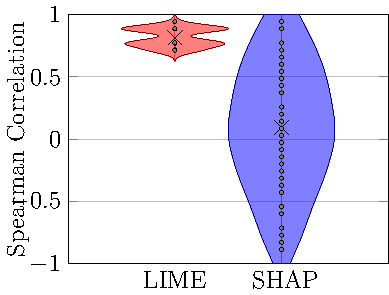
\includegraphics[width=\textwidth]{FinalFigures/sec4_3_perfect_data_spearmans_final.pdf}
        %     \caption{Relevance}
        %     \label{fig:perfect_data_model_spearmans}
        %     \end{subfigure}
        %     \begin{subfigure}{.3\textwidth}
        %     \centering
        %     %\fbox{\includegraphics[width=\textwidth,trim=0 10 70 70 mm, clip=true]{Figures/fig22.p}%{Final_Figures/fig21.png}
        %     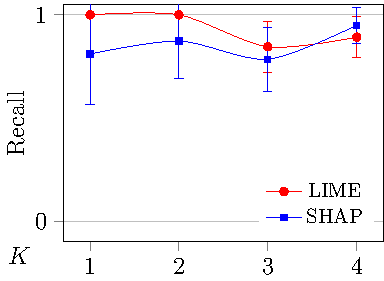
\includegraphics[width=\textwidth]{Figures/Final_Figures/sec4_3_perfect_data_recalls_final.pdf}
        %     \caption{Recall}
        %     \label{fig:perfect_data_model_recalls}
        %     \end{subfigure}
        %             \caption{SHAP and LIME when explaining an MLP with AUC $\sim .99$ trained a dataset with independent, and unconfounded features, and no unobserved features}
        %            \label{fig:perfect_data_model}
        % \end{figure}

        \subsubsection{Averaging Explanations of Different Models}
            The rate at which new machine learning models and methods appear has exploded, making it increasingly difficult for researchers to choose what model to use and ultimately explain. Coupled with the fact that each of them has hyperparameters to tune, model selection is to a machine learning researcher as was finding a route to the Spice Islands to Magellan. A straightforward way to address concerns about what black box to explain is to train many models and construct an average explanation over those models. In this way, diverse information from the hypothesis space under consideration is included in the final (averaged) explanation.%Often, but depending on the dataset, many different models can be constructed that have nearly the same predictive performance \citep{semenova22rashomon}. Each nevertheless has a distinct decision boundary and captures different correlations in the data, and so post hoc explanations of those models can still differ.
            With this in mind, we repeat the experiments of Section \ref{sec:evaluating_faithfulness} twice, once with explanations of a single model and again with the modification that concordance is calculated between the ground truth and a feature ranking constructed by averaging feature importance values over SHAP and LIME explanations of 100 unique MLPs with ROC AUC at least $.9$.
            % PUT THESE DETAILS IN APPENDIX
            %Each MLP is trained with 5 hidden layers and for 10 iterations as before, but each MLP initializes its training with a different random seed. We control for the inconsistency of the explainers by using default hyperparameters and keeping the random seed of the explainers the same. 
             
            The results of our Wilcoxon tests for improvement of data-alignment were quite different between SHAP and LIME. These differences are visualized in Figure \ref{fig:mlp_increase}. Directionality, concordance, and relevance were all significantly improved for LIME. We rejected the null hypothesis of equal sign accuracies in favor of improvement for ``cosigner", ``married", and ``sex" with respective p-values of $0.04$, $4.56e-4$, and $2.87e-7$. We rejected the null hypothesis of equal concordances in favor of improvement as the p-value was $4.21e-11$. In contrast, there was no significant change to sign accuracy for any feature (all p-values were at least $0.15$) and no significant change to concordance, as we failed to reject the null hypothesis of equal concordances with a p-value of $0.25$. Figures \ref{subfig:mlp_avg_lime_sign_accs} and \ref{subfig:mlp_avg_lime_recalls} together show that LIME was had better estimates of the $\boldsymbol{\beta}$ coefficients for ``age", ``cosigner", married, and sex.  In contrast, for SHAP, it is difficult to see any difference in directionality and concordance in Figure \ref{subfig:mlp_avg_shap_sign_accs} and Figure \ref{subfig:mlp_avg_shap_recalls}. %Our results are shown in Figure \ref{fig:mlp_increase}.
            
            %Figure \ref{subfig:mlp_avg_lime_spearmans} shows that LIME's averaged explanations had a slightly larger mean and slightly lower range while Figure \ref{subfig:mlp_avg_lime_spearmans} shows that concordance was almost unchanged for SHAP. Figures \ref{subfig:mlp_avg_lime_sign_accs} and  for LIME and \ref{subfig:mlp_avg_shap_sign_accs} and \ref{subfig:mlp_avg_shap_recalls} show that, with a few exceptions, the averaged explanations were at least as good as the explanations of a single model at identifying feature importance signs and the top-$k$ features. 
            
            %However, the strategy does not seem to be particularly beneficial for finding the top-$k$ features; the curves plotting the recall for SHAP and LIME in Figures \ref{subfig:mlp_avg_lime_recalls} and \ref{subfig:mlp_avg_shap_recalls} are nearly identical for the averaged and single explanation.%Figure \ref{fig:mlp_avg_recalls} also shows that the curves representing the relationships between $K$ and recall for $n=100$ bound the other curves from above. Therefore, this strategy appears to be effective in reducing both misalignment and inconsistency.

            This strategy can be seen as a simplified version of \citep{donnelly2023rashomon}. Instead of leveraging explanations of good models trained on one dataset, they leverage explanations of optimal decision trees or GAMs trained on bootstraps of one dataset. At the time of writing, their method is not valid for more complex models like neural networks. It also produces statistics for feature importance instead of singular feature importance values. 
    

        \begin{figure}[t!]
            \subfloat[SHAP Directionality]{%
                \raisebox{.2cm}{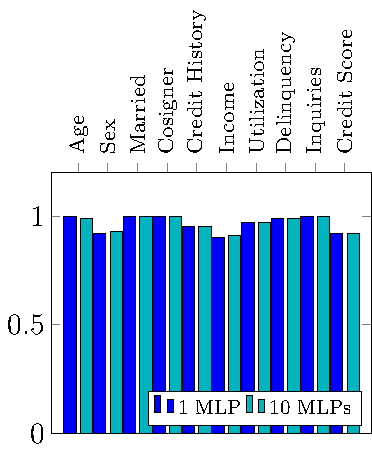
\includegraphics[width=.28\textwidth]{Figs/sec5_2_simple_mlp_avg-figure1.pdf}}%
                \label{subfig:mlp_avg_shap_sign_accs}%
            }\hspace{1cm}
            \subfloat[SHAP Concordance]{%
                \raisebox{.05cm}{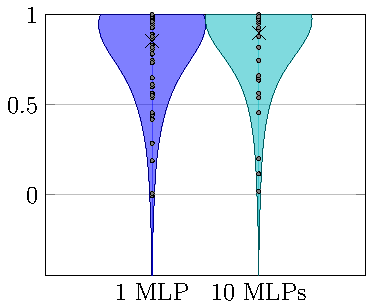
\includegraphics[width=.28\textwidth]{Figs/sec5_2_simple_mlp_avg-figure3.pdf}}%
                \label{subfig:mlp_avg_shap_spearmans}%
            }\hspace{1cm}
            \subfloat[SHAP Relevance]{%
                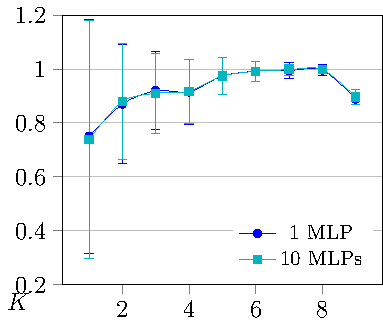
\includegraphics[width=.28\textwidth]{Figs/sec5_2_simple_mlp_avg-figure5.pdf}%
                \label{subfig:mlp_avg_shap_recalls}%
            }\\
            \subfloat[LIME Directionality]{%
                \raisebox{.2cm}{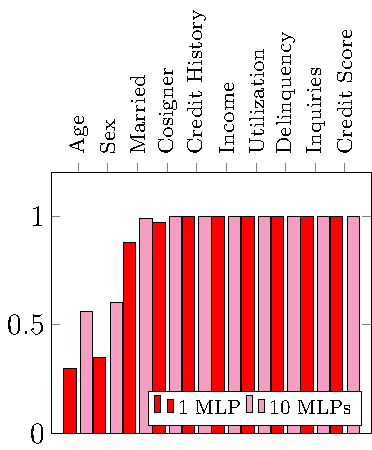
\includegraphics[width=.28\textwidth]{Figs/sec5_2_simple_mlp_avg-figure0.pdf}}%
                \label{subfig:mlp_avg_lime_sign_accs}%
            }\hspace{1cm}
            \subfloat[LIME Concordance]{%
                \raisebox{.05cm}{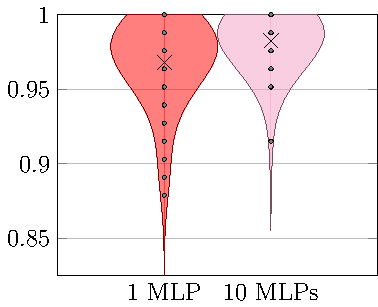
\includegraphics[width=.28\textwidth]{Figs/sec5_2_simple_mlp_avg-figure2.pdf}}%
                \label{subfig:mlp_avg_lime_spearmans}%
            }\hspace{1cm}
            \subfloat[LIME Relevance]{%
                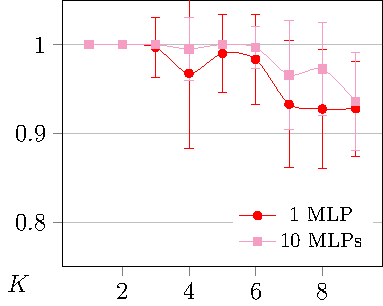
\includegraphics[width=.28\textwidth]{Figs/sec5_2_simple_mlp_avg-figure4.pdf}%
                \label{subfig:mlp_avg_lime_recalls}%
            }\\
            \caption{Comparisons of results for our three metrics for SHAP (top row) and LIME (bottom row) explanations of 1 MLP versus explanations constructed by averaging the feature importance values of 10 MLPs.}
            \label{fig:mlp_increase}
        \end{figure}
        

   
    
    \subsection{Summary and Discussion of Mitigation Strategies}
            \label{sec:summary_and_strategies}
             The main results of our mitigation experiments are that when using SHAP the Shapley values should be normalized, and when using LIME, it may be worthwhile to aggregate the explanations of many LIMEs and individual LIME explainers should have large $\nu$ and $n$. Secondarily, it may be worthwhile to seek black boxes that optimize the trade-off between complexity and predictive power and to average explanations over ensembles of explainers and/or models. 
            %It makes less sense to combine explanations of a single model than explanations of multiple models because of the idea that ``all models are wrong". 
            
            Finding common (valid) patterns within multiple black boxes is possible by aggregating explanations of those models whereas aggregations of explanations of a single black box can at best reveal the single, imperfect, pattern identified by that black box. Ignoring bias and error in the dataset, each explanation has two layers of approximation error with respect to the ground truth whereas each black box has only its own approximation error and captures different patterns in the training data. Thus, researchers may find averaging feature importance values obtained by many models both a useful and intuitive strategy\citep{dong2020variable,donnelly2023rashomon}.  %With the configuration of data and model we used, the local error rates of both SHAP and LIME were skewed to the right, implying that the mean local fidelity over samples of SHAP and LIME models can decrease as the sample size increases. However, it is difficult to validate this claim because the local fidelity of SHAP and LIME is not an especially good measure of how faithful their explanations are to $\mathcal{G}$. That averaging SHAP and LIME together did not yield a consistent and substantial advantage is likely due to the simplicity of the technique. For this reason, we suggest that more research be done on this topic. 
            
            Summing up, researchers who would like to investigate the importance and impact of features in a data generating process may find exploring the following general strategy useful. First, the choice of explainer(s) used for the strategy should be guided by user preference for the types of feature importance outlined in Section \ref{sec:theoretical_considerations}. For example, LIME should be preferred to SHAP if $\boldsymbol{\beta}$ is preferred to $\boldsymbol{\beta}(\boldsymbol{\xi}-\bar{\mathbf{x}})$ as the ground truth feature importance representation.  %construct average explanations over a collection of good LIME explanations of good models. If situational importance is more suitable than theoretical importance for the application, researchers should instead average over SHAP explanations of good models. 
            Next, when starting the prediction stage, the dataset should be pre-processed to remove highly correlated features\footnote{If possible, adjustments can be made to account for confounding. Tools like E-values\citep{gaster2023quantifying} and Pearl's backdoor criterion can be used for this purpose.}% The causal graph can be estimated using Bayesian Networks if sufficient domain knowledge is available.}
            Having pre-processed the data, researchers are encouraged to train $B\geq 1$ black box models with simple enough decision boundary/separating surface to not lose too much predictive performance compared to more complex models. \footnote{Ideally, Rashomon sets of models would be constructed and the simplest models in them would be collected. However, at the time of writing, this is only possible for decision trees and GAMs.} To construct an explanation for the predicted outcome of an instance, the results of multiple explainers can be aggregated by, e.g., averaging the feature importance values over the component explainers. Doing this for each of the $B$ models, $B\cdot E$ explanations in total are used to produce a final explanation for an instance.
            
            % \section{Testing the Recommended Pipeline}
            %     We will demonstrate the efficacy of our recommended pipeline by benchmarking it against a baseline pipeline on five new simulated datasets. The five datasets are have the following ground truths, which have increasing complexity. $\mathcal{G}_1$ is linear, but includes nonlinear transformations of $x$. $\mathcal{G}_2$ includes nonlinear transformations of the $x_i$ as well as an interaction term. $\mathcal{G}_3$ includes features which are correlated through another set of observed features. $\mathcal{G}_4$ has unobserved confounding. $\mathcal{G}_5$ additionally has an interaction term.  
            
            %     \begin{enumerate}
            %         \item  $\mathcal{G}_1(x) = \mathds{1}[\sum_{i=1}^{10} \lambda_i log(x_i) > c_1]$ where $\lambda_i \in (0,1)$ and $x_i \sim \mathcal{U}(1,10)$ $\forall i$
            %         \item $\mathcal{G}_2(x) = \mathds{1}[\mathbf{\Sigma}(x_1x_2 + cos(x_2) + min(x_3,0) + exp(x_4/4) + x_5^2/2) > .5]$ and $x_i \sim \mathcal{U}(-1,1)$
            %         \item $\mathcal{G}_3(x) = \mathds{1}[\mathbf{\Sigma}(x_1 + 2x_2 + x_3/3 + 2x_4/3 + x_5)>c_4]$ where $x_1,x_2,x_3 \sim \mathcal{N}(0,1)$, and $x_4 = 2 +  z_1$, $x_5 = 2 + 3 z_3$ where $z_3 = .8 z_1 + \sqrt{1-.8^2}z_2$ and $z_1\sim \mathcal{N}(1,1)$ and $z_2 \sim \mathcal{N}(2,9)$ with $z_1,z_2$ in the training data
            %         \item $\mathcal{G}_4(x)$ the same as $f_4(x)$ but without $z_1,z_2$ in the training data
            %         \item $\mathcal{G}_5(x) = \mathds{1}[\mathbf{\Sigma}(2x_1x_2 + \frac{1}{sin(x_3)} + 2x_4/3 + x_5)>c_5]$ where $x_1,x_2,x_3 \sim \mathcal{N}(0,1)$, and $x_4 = 2 +  z_1$, $x_5 = 2 + 3 z_3$ where $z_3 = .8 z_1 + \sqrt{1-.8^2}z_2$ and $z_1\sim \mathcal{N}(1,3)$ and $z_2 \sim \mathcal{N}(.5,4)$ without $z_1,z_2$ in the training data. \textcolor{red}{Fenglu should pick $c_5$ such that the target is highly imbalanced.}
            %     \end{enumerate}
                
                
            %     Our baseline pipeline will be represented by a default LIME explanation of an MLP with a ROC AUC of about $.8$. To represent our recommended pipeline, we construct an average explanation for each applicant using the explanations of 10 MLPs with AUC $\geq .9$ by 10 LIME explainers that correctly classify the applicants' loan decisions. We attempt to find the minimum complexity that allowed the MLPs to attain AUC values that exceeded $.9$ to avoid needless model complexity and overfitting. 



\subsection{Case Study: Replicating Econometric Findings}
    \label{sec:case_study}
    To validate our efficacy of our mitigation strategies and illustrate how they could be employed in practice, we will compare how well two combined strategies Replicating insights from an econometric paper on the approval of home loan applications \citep{bane2006econometric} against two baselines. The home loan dataset is publicly available and originates from a study by the Federal Reserve Bank of Boston \citep{hunter1996cultural}. We take the ground truth $\boldsymbol{\beta}$ underlying this dataset to be the coefficients of the logistic regression model obtained in the analysis of \cite{bane2006econometric}. This is justifiable because econometric modeling is equipped to capture $\boldsymbol{\beta}$. The linear ground truth model derived from their logistic regression model appears in Equation \ref{eqn:econ_gt}. The meanings and ranges of each feature appear in Appendix Table \ref{tab:case_study_features}.  %We will use the logistic regression coefficients to evaluate SHAP and LIME explanations in the same manner as has been done throughout this paper. We suppose that the logistic regression coefficients have the correct signs and magnitudes relative to each other, not that the logistic regression itself is the true causal model underlying home loan approvals in Boston. 

    Our two combined strategies are versions of the general strategy outlined in Section \ref{sec:summary_and_strategies} tailored to SHAP and LIME. We will perform the following comparison to evaluate them. First, we split the dataset into 80\% training data and 20\% testing data. Then we train 10 MLPs with test set AUC that are all near $.92$. The LIME variant of the strategy uses all $B=10$ MLPs and $E=10$ LIME explainers for each MLP. Each LIME explainer has $\nu=n=10000$. Because SHAP is (essentially) deterministic and the MLP averaging strategy did not significantly increase directionality and concordance for SHAP, we use $B=E=1$ and normalize the Shapley values. Baseline explanations come from explanations of one MLP with accuracy $.86$, ROC AUC $.93$ with individual SHAP and LIME explainers both using default settings. 
    
    %\begin{tcolorbox}[title = Econometric Ground Truth Model $\mathcal{G}$]
    \begin{equation}
    \label{eqn:econ_gt}
    \begin{split}
        \mathcal{G}(X) =.8 + 3.5\cdot \text{good credit} + 4.7\cdot \text{purchaser type} -4.4 \cdot \text{PMI approved} - .4 \cdot \text{multi family} \\ -2.5 \cdot \text{unver} + .9 \cdot \text{fixed rate} - 1.4 \cdot \text{bankruptcy} - .9 \cdot \text{value rate} - .03 \cdot \text{debt rate} \\- .7 \cdot \text{old} + .8 \cdot \text{married} - .8 \cdot \text{gift}
    \end{split}
    \end{equation}
    %\end{tcolorbox}
    %\subsection{Baseline Performance}
    %Figure \ref{fig:econ_cmp} compares the explanation quality  for 100 applicants from the baseline pipeline and recommended pipeline. %In the Appendix, we show also compare results for importance sign accuracy, Spearman rank correlation, and recall.

    Both the SHAP and LIME variants of our general strategy generally had results which improved upon the baseline in at least one respect. Indeed, our strategy applied to LIME significantly improved concordance overall, significantly improved directionality for ``fixadj" and ``old", significantly improved relevance for the top 2 and 3 features. It had significantly worse directionality only for ``vr" and ``obrat", and significantly worse relevance for features not in the top-4. Our strategy applied to SHAP significantly improved directionality for all features except ``fixadj" and ``gift", significantly improved concordance, and significantly improved relevance for all $k\neq 1,11$. 
    
    %Figure \ref{fig:econ_cmp} visualizes the results. The directionality values from our recommended strategy with SHAP and LIME were at least as good as those from the baseline for all features except ``pubrec" (bankruptcy filed) for LIME and ``vr" (value rate) for SHAP (see Figures \ref{subfig:econ_lime_sign_accs} and \ref{subfig:econ_shap_sign_accs}). The concordance plots for both SHAP and LIME in Figures \ref{subfig:econ_shap_spearmans} and \ref{subfig:econ_lime_spearmans} show that the recommended pipeline rankings were generally more faithful than the most faithful explanations from the equivalent baseline. Finally, it can be seen from Figures \ref{subfig:econ_lime_recalls} and \ref{subfig:econ_shap_recalls} that the recommended strategies using SHAP and LIME both have substantially higher relevance for all $k\neq 1,\ 10,\ 11$.
     
% \begin{figure}[!h]
% \centering
%     \begin{subfigure}[t]{0.28\textwidth}
%     \centering
%     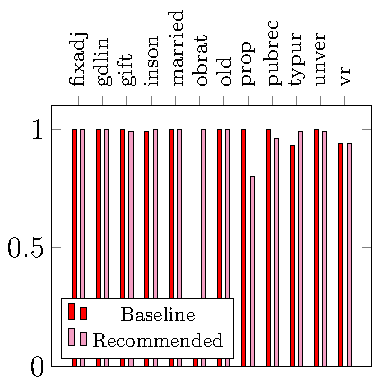
\includegraphics[width=\textwidth]{Figs/econ_cmp-figure0.pdf}
%     \caption{Directionality} \label{fig:econ_cmp_sign_accs}
% \end{subfigure}\hspace{1cm}
% \begin{subfigure}[t]{0.28\textwidth}
%     \centering
%     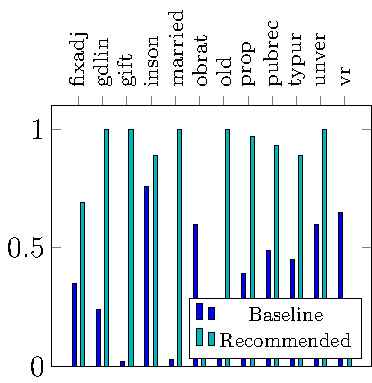
\includegraphics[width=\textwidth]{Figs/econ_cmp-figure1.pdf}
%     \caption{Relevance} \label{fig:econ_cmp_spearmans}
% \end{subfigure}\hspace{1cm}
%  \begin{subfigure}[t]{0.28\textwidth}
%     \centering
%     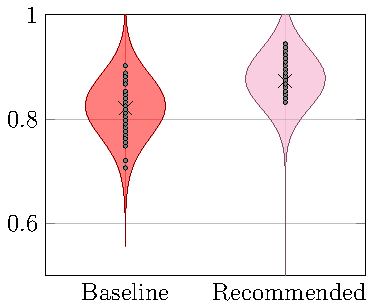
\includegraphics[width=\textwidth]{Figs/econ_cmp-figure2.pdf}
%     \caption{Recall}
%     \label{fig:econ_cmp_recalls}
% \end{subfigure}
% \caption{Improvements due to use of recommended pipeline instead of one without any of our mitigation strategies}\label{fig:econ_cmp}
% \end{figure}


        \begin{figure}[t!]
            \subfloat[SHAP Directionality]{%
                \raisebox{.2cm}{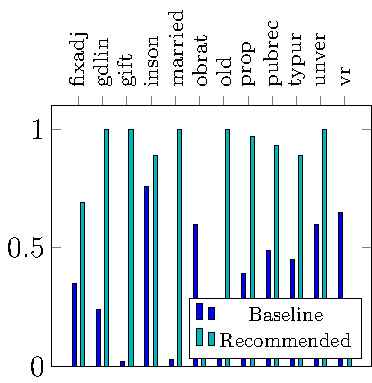
\includegraphics[width=.28\textwidth]{Figs/econ_cmp-figure1.pdf}}%
                \label{subfig:econ_shap_sign_accs}%
            }\hspace{1cm}
            \subfloat[SHAP Concordance]{%
                \raisebox{.05cm}{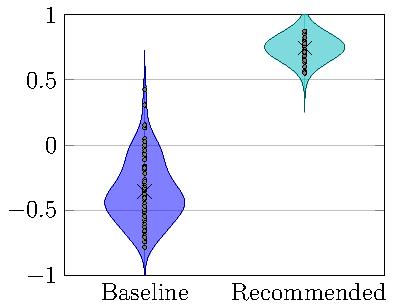
\includegraphics[width=.28\textwidth]{Figs/econ_cmp-figure3.pdf}}%
                \label{subfig:econ_shap_spearmans}%
            }\hspace{1cm}
            \subfloat[SHAP Relevance]{%
                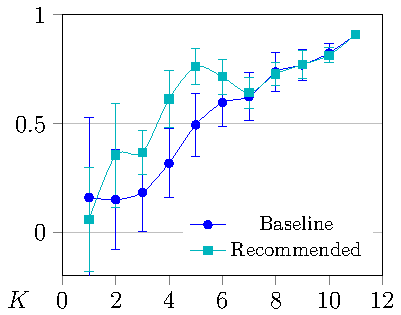
\includegraphics[width=.28\textwidth]{Figs/econ_cmp-figure5.pdf}%
                \label{subfig:econ_shap_recalls}%
            }\\
            \subfloat[LIME Directionality]{%
                \raisebox{.2cm}{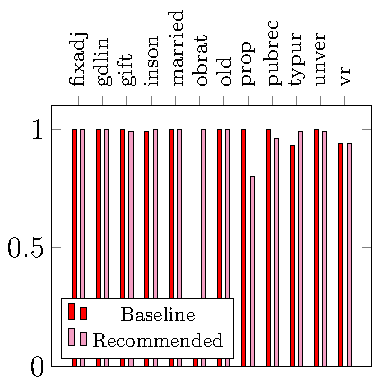
\includegraphics[width=.28\textwidth]{Figs/econ_cmp-figure0.pdf}}%
                \label{subfig:econ_lime_sign_accs}%
            }\hspace{1cm}
            \subfloat[LIME Concordance]{%
                \raisebox{.05cm}{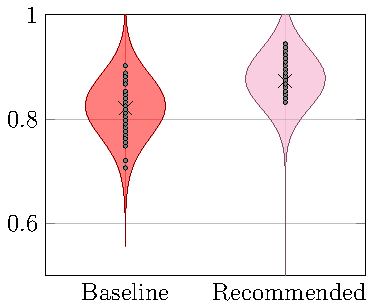
\includegraphics[width=.28\textwidth]{Figs/econ_cmp-figure2.pdf}}%
                \label{subfig:econ_lime_spearmans}%
            }\hspace{1cm}
            \subfloat[LIME Relevance]{%
                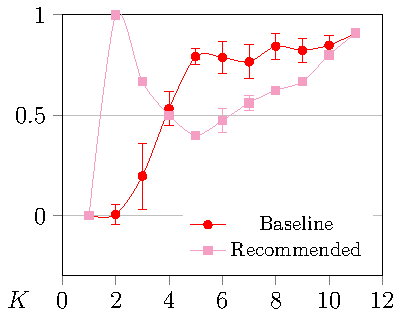
\includegraphics[width=.28\textwidth]{Figs/econ_cmp-figure4.pdf}%
                \label{subfig:econ_lime_recalls}%
            }\\
            \caption{Improvements due to use of recommended pipeline instead of one without any of our mitigation strategies}\label{fig:econ_cmp}
        \end{figure}
    



\section{Discussion and Conclusion}
    \label{sec:discussion}
    As post hoc explanations are gaining popularity in business research, we found an alarming trend of using them to make claims about the underlying variable relationships in the data. In our survey of 150 business papers, we found 42\% of papers use LIME or SHAP for this purpose. However, the validity of this use of post hoc explanations has not been studied in the literature. 
    This paper is the first effort towards this purpose. 
     In the following sections, we will summarize our findings and give some parting advice for the use of post hoc explainers for obtaining managerial insights in business research. 

    %    
    %In this paper we have introduced and investigated issues of misalignment and inconsistency of post hoc explanations. Our thorough literature review uncovered that business researchers using post hoc explanations value data-alignment. Thus we have contributed to the business literature by providing both theoretical and empirical evidence that the two most popular explainers, LIME and SHAP, often produce misaligned explanations. Notably, we proved that SHAP is inherently unsuitable to infer information about $\boldsymbol{\beta}$. %We have also identified various factors that contribute to misalignment and inconsistency. 
    We also contribute to the business literature by proposing some simple and intuitive mitigation strategies which we found to benefit explainer data-alignment to varying extents.

    \subsection{Main Findings}
        Our paper contributes several important findings to the use of post hoc explanations in business research.

        First, through an extensive literature review, we found that the use of post hoc explanations to infer information about the data is quite prevalent. In the 150 papers we reviewed, 63 used SHAP or LIME to draw conclusions about the $X\rightarrow Y$ relationship instead of the $\mathcal{M}(X)\rightarrow Y$ relationship. Such use deviates from the intended purpose of post hoc explainers: they are designed to explain the machine learning model, not to infer any information from the data. Identifying this misuse of post hoc explanations is an important contribution of this paper. Note that while post hoc explanations have been first introduced and widely used in the machine learning community, the issue we discuss in this paper is less of a concern for that community because computer scientists are more interested in model explanations. Post hoc explainers are used to understand a machine learning model's behavior in order to diagnose and debug the model. However, social scientists and business researchers try to understand the data and the underlying phenomena, making this issue more prominent in business research.
        % Using simulated loan application datasets, we produced ground truth application approval mechanisms $\mathcal{G}$ along with MLP approximators $\mathcal{M}$ trained on $\mathcal{G}$ and investigated how well popular post hoc explainers could recover the $\boldsymbol{\beta}$ underlying $\mathcal{G}$. This investigation was motivated by the need to assess the utility of post hoc explainers to business researchers and managers. We used our results from the investigation using simulated data to propose a set of mitigations that would worth exploring in practice. Finally, we tested the efficacy of this set of mitigations in a test to see if we could use LIME to reproduce the results of an econometric study of home loan applications. We found that although it was far better to use them than not, the resulting explanations were still imperfect. 

        % When evaluating the ability of the two most popular post hoc explainers, SHAP and LIME, to extract faithful insights from both real and simulated data, we identified the following issues that are cause for concern for researchers interested in $\boldsymbol{\beta}$ estimation problems using post hoc explainers. 

       Second, we provide both theoretical and empirical evidence that SHAP and LIME explanations are, in fact, not data-aligned. In our investigation, we discovered that SHAP and LIME incorrectly represent the signs and relative importance of the marginal effects of the explanatory variables used to train the models they explain. As shown in Section \ref{sec:causes_of_misalignment}, SHAP and LIME tend to be data-misaligned even in scenarios where they explain an accurate machine learning model trained on data whose features are mutually independent and whose target is derived from a simple linear ground truth model (scenarios which are, in a sense, ideal). This observation suggests a need for caution when interpreting variable relationships based on post hoc explanations. It opens up a dialogue about the complexities of deriving accurate insights from such models, contributing to a deeper understanding of their limitations and paving the way for future research in this area. In light of these insights, it may be beneficial for the academic community to revisit prior analyses that have relied heavily on post hoc explanations. This reassessment could ensure that interpretations and conclusions drawn from such models are robust and reflective of their underlying dynamics. Our findings underscore the importance of continuous critical evaluation in the field, especially as we seek to refine our understanding and application of these explanatory tools. %Our finding is echoed in other recent studies that compared the  \cite{baghdasaryan2021comparison}
        
        Third, we find that the reason for the data-alignment is different for SHAP and LIME. Achieving data-alignment using unmodified SHAP feature importance values is inherently impossible due to the nature of Shapley values. Shapley values represent a feature's contribution to a prediction by considering not only the feature's marginal effect but also its value and the influence of other variables within the explanation process. In the particular case where SHAP explains a linear model, the vector of Shapley values is given by $\boldsymbol{\beta}(\boldsymbol{\xi}-\bar{\mathbf{x}})$, diverging from a direct representation of $\boldsymbol{\beta}$. Conversely, LIME's data-alignment arises from the mechanics of its default ridge regression approach. Our analysis, supported by Theorem \ref{thm:lime_thm}, indicates that LIME could achieve data-alignment by avoiding the discretization of numerical inputs, sampling many points for its synthetic regression problem, and opting for a significantly larger bandwidth than the default. Yet, even with these adjustments, common properties of real-world data such as correlated variables often hinder the attainment of data-alignment. Nonetheless, it is noteworthy that our evaluations generally reveal \textit{LIME to provide explanations of higher concordance and relevance compared to SHAP}.
 
        
         Finally, we identify several mitigation strategies that show promise in enhancing the data-alignment of explanations across various stages of the explanation pipeline. These strategies, validated through empirical testing, offer significant improvements in aligning explanations more closely with marginal effects. However, it is important to acknowledge that none of the strategies can guarantee complete congruence with marginal effects. This absence of a full guarantee means that while explanations may sometimes align closely with the marginal effects, they cannot reliably do so, thus calling for great caution when researchers use them. Such a scenario potentially restricts the applicability of post hoc explanations, as users may remain uncertain about the extent to which these explanations accurately mirror the underlying the marginal effect structure. This limitation underscores the need for cautious interpretation and application of post hoc explanation methods in practical scenarios.
        
        
        % \textcolor{red}{what else did we *find*?}

            
        % Second, users must deal with inconsistent explanations because not only do e.g. SHAP and LIME each produce different explanations for the same outcome, but LIME may produce self-contradictory explanations of the same outcome. How to select an explanation(s) from the myriad available from different combinations of accurate black box models, explainers, and explainer hyperparameters is up to the user, but the mitigations suggested in this paper can help users make more informed decisions.%but robustness checks like those presented in this paper can be used to estimate how confident users can be in their selection(s). 



        % stuff re: prescriptive removed
        %Our main finding regarding prescriptive insights is that LIME, SHAP, and DiCE seem to only be of use for actionable recourse a minority of the time. When tasked with generating new application profiles for denied loan applicants, those new application profiles would be approved by $\mathcal{G}$ less than 50\% of the time. %\textcolor{blue}{May need to be removed!! We showed that... DiCE, a counterfactual explainer (as opposed to an attributive one like SHAP and LIME) was always able to produce new application profiles for rejected loan applicants that would lead to approval in our experiments (for a sufficiently small sparsity parameter). }For DiCE, if we restrict the range of feature variations (within one standard deviation) and the number of features allowed to vary, it can only provide prescriptive insights to a small number of denied applicants.
        
    % \subsection{On Mitigation Strategies}
    %     We proposed some intuitive mitigation strategies for the issues of unfaithful and inconsistent explanations. Each of them was effective with respect to at least one of our three metrics. However, none of them were fully effective solutions that would guarantee that practitioners could confidently use LIME or SHAP for $\boldsymbol{\beta}$ estimation and econometric modeling. Thus, we encourage cautionary usage of SHAP and LIME and to consider exploring the usage of our mitigation strategies in efforts to obtain more data-aligned explanations. 
        
    %     Our principal finding regarding faithfulness was that SHAP has no chance at data-alignment unless its Shapley values are normalized by the difference between feature values and feature means. We also found that the most important strategy for increasing the faithfulness of LIME is to disable discretization of numerical features and to make the number of samples and kernel bandwidth it uses for weighted ridge regression large. 
        
    %     %We found some success in increasing the faithfulness of an explanation of a model $\mathcal{M}$ to the ground truth $\mathcal{G}$. As expected, whether $\mathcal{M}$ and $\mathcal{E}$ can correctly predict decisions from $\mathcal{G}$ affects how faithful their explanations are to $\mathcal{G}$. In addition to ensuring low generalization error of $\mathcal{M}$, we also noted that ensuring that $\mathcal{M}$'s training data without correlated or confounded features resulted in remarkably better results than otherwise. However, it is important to note that the explanations were still usually imperfect even though the model and data were ideal. 
    
    %     To combat inconsistency, we proposed techniques to construct aggregate explanations that are better on average than individual explanations. These strategies worked by  averaging feature importance values obtained from explanations obtained from different combinations of models and explainers. The motivation behind these averaging strategies was that they address uncertainty in the choices users need to make by aggregating the many combinations of models and explainers that are the root of the uncertainty. In addition to addressing inconsistency, these strategies resulted in statistically significant improvements in at least directionality, concordance, or relevance. 

    %     In exploring mitigation strategies, we did not find evidence that LIME or SHAP can be used in a way that makes them suitable alternatives to traditional econometric modeling. Although our recommended strategies for SHAP and LIME compared favorably to their associated baselines in a test to reproduce results an actual econometric study of loan approval, they were unable to consistently extract the $\boldsymbol{\beta}$ that the econometricians found. 

%\textcolor{red}{add in the discussion that althgouh we do not know when the explanation aligns with beta, we can identify when they do not: just run  pipeline multiple times with different split of data and different ML model, if the results do not agree, it is a clear sign that the beta-alignment is low}
    
    
    \subsection{On the Use of post hoc Explanations}
  We want to emphasize that this paper focuses on the issue of using post hoc explanations to make inferences about the ground truth information in $\mG$ that generates the data. We do not explore their use in explaining the machine learning model $\mM$ or its predictions $\mathcal{M}(X)$, which is the primary intended purpose of post hoc explainers. However, it is important to note that even this intended use of post hoc explainers raises some concerns \citep{garreau2020looking,alvarez18robustness,kumar20shap,jacovi2023diagnosing}. For the scope of this paper, our discussion is solely focused on inferring ground truth information from $\mathcal{G}$ through the explanations for $\mathcal{M}$.

    \subsubsection{General Usage}
      While this paper recommends against using post hoc explanations to make any definite claims about marginal effects, it does not mean that post hoc explanations cannot be used at all. Instead of using them as a tool to \textbf{validate} hypotheses and viewing the explanations as evidence, we propose to use post hoc explanations to \textbf{propose} hypotheses that can guide subsequent efforts after they are corroborated.  As a preliminary step, researchers can use the level of inconsistency between explanations of models trained on different splits of the data to gauge data-alignment, viewing explanations which do not share common patterns found the collection of explanations as an indication of its implausibility. Following the preliminary step, an ideal usage of a hypothesis which is deemed to be plausible and interesting would be to empirically validate it through e.g. randomized trials and with collaboration with domain experts. If this were not presently feasible, researchers could at least call on domain experts to validate the hypothesis \citep{donnelly2023rashomon} or do further analyses themselves using tools which are more suited to ascertain causal relationships. For example,  \cite{zhang2023can} follows up their search for important features for restaurant survival using SHAP by using causal forests to estimate the treatment effects of those features. Similarly, \cite{hanauer22boosting} use traditional regression as a trusted baseline that they compare SHAP explanations to. 
      Additionally, as was done in \cite{tang2024china}, plausible post hoc explanations can be used to aid classical regression analyses as a feature selection method. That is, researchers can opt to use only those features which are said to be important by a post hoc explainer(s) in their regressions but should keep in mind that those features may not actually be important to $\mathcal{G}$. 
    
    
    
% \textbf{How to Make Fruitful use of post hoc Explainers}.
% \cite{Usc paper and the other paper using shap to select features}
%  Model-agnostic post hoc explainers certainly have legitimate use cases, but due to the nature of real business datasets and stakes associated with business problems, we urge the business community to use them with caution and with tempered expectations. The problems of data-misalignment and inconsistency make it difficult for researchers to choose explanations in a principled fashion and ascertain their truth value. Thus, without sufficient domain knowledge or evidence, a researcher can neither believe nor trust the content of a post hoc explanation, nor use it to make inductive inferences. In such a context, the only truly principled view of a post hoc explanation is as a hypothesis. 
 

    
    %Then their explanations can be used as a basis for more rigorous analysis. For example, the treatment effects of features identified as important by the explainers can be estimated using causal forests \citep{zhang2023can}.   
    
        %The outline given in Section \ref{sec:summary_and_strategies} can undoubtably be improved and tailored to user-specific situations, and so is worth expounding. We do so below, and provide additional information that could be useful in different use-cases. 


        %During Prediction stage, before even beginning model development, users should use correlation analysis and any available domain knowledge to identify correlated or colinear features, and then decide whether to drop them from the dataset. % attempt to understand the causal graph associated with their problems and employ statistical tests of unconfoundedness assumptions. With this knowledge, users need to decide whether it is worthwhile to use post hoc explainers instead of randomized experiments. If so, the data should be pre-processed to have the desirable properties we have outlined previously. Domain knowledge and knowledge of the causal graph are useful for this purpose~\citep{zhao2021causal}.% to remove redundant features, causal descendants of a collinear pairs of causally linked features. Confounders should be controlled for if possible.
        %Then, unless users are only interested in explaining a particular black box model, we propose that many be generated and used for explanations. This is due to the Rashomon Effect\citep{semenova22rashomon}, which states that models (interpretable or otherwise) with approximately the same predictive performance will represent different relationships of the input features to the target. In other words, equally good models will have different (possibly conflicting) explanations and interpretations. In the best case, users could leverage explanations entire Rashomon sets of good models from specified model classes and training datasets. We showed that this technique was useful when averaging explanations over a rather small set of MLPs with high ROC AUC using LIME explainers which correctly classify the input being explained. Additionally, because we found that the complexity and generalization error of $\mathcal{M}$ was related to post hoc explanation quality and variability, we propose that researchers gather as much training data as feasible.%.qasw11111 and take care not to overfit their models. %Overfitting is especially detrimental because the complexity of the decision boundary of $\mathcal{M}$ contributes to the instability of the explainer. After all, even a perfect explainer for a model which is highly locally nonlinear must be unstable. Thus, needless complexity in a decision boundary due to overfitting could cause an explainer of the decision function to be unstable when it should not be.  

       
        %When starting the explanation stage, users should keep in mind that post hoc explanation can be accidentally misused due to a fundamental misunderstanding of the explainer. For example, \cite{kaur2020interpreting} showed that practitioners misused explanations due to having an incorrect understanding of Shapley values. \cite{jacovi2023diagnosing} also discusses the possibility of users coming away with an incorrect understanding of incomplete explanations because they fill in missing information with their own biases. Users should ensure that they have a complete understanding of how explainers they intend to use work and how their biases may affect their understanding of the explanation. Having done this, we recommend researchers to view post hoc explanations simply as hypotheses and avoid using them to assert novel findings about $\mathcal{G}$ or claiming that they confirm existing hypotheses. 
        
        %As we have discussed, due to the problems of misalignment and inconsistency, researchers should not trust that a single explanation from any explainer applied to any black box model is true unless they can corroborate the explanation. Ideally, explanations would be corroborated using domain knowledge. Otherwise, users could consider comparing the explanations with patterns found in inherently interpretable models or use explainers only for exploratory analyses that are followed up with more rigorous analysis. For example, we recommend that researchers use robustness checks to figure out how confident they can be in the variability of explanations, and select or aggregate explanations from among the large set of explanations created during the robustness checks. 

\subsubsection{Can SHAP be Used as an Alternative to Econometrics Methods?}
    We address whether SHAP can be used as an alternative to traditional econometric modeling because this type of usage was a pattern we found in our literature review. That is, researchers were motivated to use SHAP explanations of an ML model to obtain feature importance values because of perceived advantages XAI has over regression analysis. The most commonly cited advantage is that, unlike traditional least squares regression methods, SHAP explanations automatically include nonlinearities and interactions. 
    
    The following works exemplify the aforementioned usage pattern. \cite{berger2023supply} describes their motivation to use SHAP by asserting that SHAP can provide similar economic insights to pooled OLS \emph{and} capture the non-linear impacts of features. \citep{srivastava23energy}, which expresses the desire to use and explain ML models with SHAP in order to find factors driving energy consumption because ML models can ``detect highly complex interactions between drivers of energy consumption", is an example of this. Furthermore, \cite{zhou23consumption} says that XAI methodology is appealing because it does not necessitate ``...the construction of more intermediate variables and complex statistical analysis". Similarly, \citep{banulescu2023practical} are drawn away from logistic regression because it suffers when a large number of predictors are used. \cite{hanauer22boosting} choose not to use traditional linear regression analysis used for fundamental stock analysis and instead explain random forest and XGBoost models because the ML models deal with non-linearities, interactions, and noisy features. \cite{li24roles} makes inferences about bike sharing by explaining their XGBoost model instead of examining the coefficients of their linear regression because the XGBoost had better predictive performance. 

    Authors often computed the average of the absolute Shapley values over their test set and used the results as measures of global feature importance. \cite{lenaers23rent,maeng23vr,guenther2023useful} are all examples. This obviously comes at a cost of losing any indication of the directionality of impact by features. However, they must do this because the means of signed Shapley values should be 0 due to Equation \ref{eqn:shap_gt}. This is usually the case empirically; \citep{lenaers23rent,maeng23vr,jiang24churn} all show scatter plots of the signed Shapley values of each feature over their dataset and the empirical distributions of the Shapley values are almost always centered at 0. Equation \ref{eqn:shap_gt} implies that the expected absolute Shapley value for feature $X_j$ is proportional to $\beta_j$, but also a function of the mean and standard deviation of $X_j$. So, unless all of the $X_j$ are identically distributed, the expected absolute Shapley values may not be comparable for the sake of relative importance in the same way as the $\beta_j$. In other words, a ranking of the average absolute Shapley values may be different than the ranking of the $\mid \beta_j\mid$.  %For example, if $\beta_1=1$ and $\beta_2=2$ with $X_1\sim\mathcal{N}(\mu_1=100,\sigma_1=1)$ and $X_2\sim \mathcal{N}(\mu_2=0,\sigma_2=\frac{1}{10})$ that are viewed as important in the sense of the effect of a unit increase, the expected absolute Shapley value for $X_1$ is larger than the expected absolute Shapley value of $X_2$ even though $X_2$ is more important than $X_1$ because $\beta_2>\beta_1$:
    % \begin{equation*}
    %     \mathds{E}[\mid \beta_1(X_1-\mu_1)\mid] = \sqrt{\frac{2}{\pi}} > \mathds{E}[\mid \beta_2(X_2-\mu_2)] = \frac{1}{5}\sqrt{\frac{2}{\pi}}
    % \end{equation*}

\subsection{Final Remarks}% and Future Work}
This paper aims to highlight the issue with a use of post hoc explanations that we identify as inappropriate. To demonstrate the seriousness of this problem, we show that it occurs even in the simplest context, where the ground truth $\mathcal{G}$ is linear. Even in this simple case, SHAP and LIME produce misaligned explanations. We expect that in more realistic scenarios their performance can only be worse. Real decision processes are often non-linear and involve feature interactions and unobservable features; naturally, these added complexities should reduce the efficacy of SHAP and LIME, making it even more challenging to obtain data-aligned explanations. Given the uncertainty regarding the validity of post hoc explanations, researchers should view them skeptically and consider them as hypotheses rather than definitive claims about reality. 


 
 % When feasible, we advocate for intrinsically interpretable models to be used instead. %When data have unobserved confounders, randomized experiments should be used to identify treatment effects.


    % reword to remove word MISUSE; need to say instead that users get incorrect misunderstanding
    %Throughout this paper, we have shown how and why the use of post hoc explainers could lead to confusion for business researchers and bad decision making for businesses. Our experiments demonstrated SHAP and LIME's inability to produce consistent and faithful explanations. Possible consequences of this include businesses or customers trying to improve upon some outcome, which could waste time and resources by adjusting for an irrelevant feature that LIME or SHAP implied was important, or even worsen the outcome they were trying to improve. On the surface, model-agnostic post hoc explainers are attractive because they are easy to use and applicable to any model with any dataset. However, their propensity toward unfaithful and / or inconsistent explanations decreases their efficacy. Due to the stakes involved with understanding business problems, post hoc explainers should only be used with great caution. 
        

% Acknowledgments here
\ACKNOWLEDGMENT{The authors gratefully acknowledge the existence of
the Journal of Irreproducible Results and the support of the Society
for the Preservation of Inane Research.}


% References here (outcomment the appropriate case)

% CASE 1: BiBTeX used to constantly update the references
%   (while the paper is being written).
%\bibliographystyle{informs2014} % outcomment this and next line in Case 1
%\bibliography{<your bib file(s)>} % if more than one, comma separated

% CASE 2: BiBTeX used to generate mypaper.bbl (to be further fine tuned)
%\input{mypaper.bbl} % outcomment this line in Case 2

%If you don't use BiBTex, you can manually itemize references as shown below.


\bibliographystyle{informs2014}
\bibliography{refs}

\newpage

% dimensions finds only 206 but indexes preprints
% scopus finds over 400 but doesn't index preprints
%% preprint not necessary
% need to ensure that the papers are actually explaining a black box
% e.g. tong will anonymize my quotations
\section{Appendix}
    The appendix contains additional details and experiments. It begins with information about how we conducted our literature review and how we judged papers for inappropriate use of explainers in Appendix Section \ref{apx_sec:lit_review}. We then provide all details relevant for Section \ref{sec:causes_of_misalignment}. First, we give proofs and experimental justification for theoretical claims in Appendix Section \ref{apx_sec:proofs}.
    Then we detail the experimental designs used in our investigation of correlation and predictive performance in Appendix Section \ref{apx_sec:misalignment_exp_details}. All  We expound upon the problem of explainer inconsistency in Appendix Section \ref{apx_sec:inconsistency} using experiments that demonstrate how and why it occurs. The next part of the Appendix is about our mitigation strategies. Appendix Section \ref{apx_sec:mitigation_details} details our hypothesis testing framework for investigating whether a strategy improves over a baseline pipeline. Appendix Section \ref{apx_sec:additional_mitigations} demonstrates some additional mitigation strategies that we tried that were less effective than the ones in the main body of the paper. Appendix Section \ref{apx_sec:econometric_details} has details about the dataset we used in our econometric case study. Finally, we give the results of a repetition of all experiments in the main body of the paper using a synthetic direct marketing example in Section \ref{apx_sec:marketing}
    
    \subsection{Literature Review}
        \label{apx_sec:lit_review}
        As part of our literature review process, we cataloged papers at the intersection of business and explainable machine learning. We used SSRN and Web of Science to search for publications citing at least one of LIME~\citep{ribeiro16lime} or SHAP~\citep{lundberg17shap} and have either ``LIME" or ``SHAP" appear in the body of the paper.  The results were filtered by topics related to business, such as management, economics, supply chain \& logistics, operations research \& management science, etc. We also searched each of the INFORMS journals for papers satisfying the same criteria. Then we closely examined 150 papers on the top of the list returned by the search. Out of these papers, \textcolor{red}{92\%} used SHAP and \textcolor{red}{9\%} used LIME. %the following Web of Science topics: transportation, management, economics, supply chain \& logistics, economic theory, and operations research \& management science. Marketing does not appear in the table because Web of Science does not include it as a distinct category among business adjacent fields. Figure \ref{fig:citation_count_graph} shows how the frequency of such papers has increased over time. 
        % Figure \ref{fig:treemap} shows the breakdown of the papers we identified by category. %index any such papers that cited WachterCF~\citep{wachter17wachtercf} or DiCE~\citep{mothilal20dice}.

        % make paragraph or table with prototypical language forms
        % labeled with relevant metric
        % 10 examples of each
        % quotations without citation 
        We took a close look at these papers and characterized the papers' use of explainers by following three steps. First, we checked if the paper used SHAP or LIME to explain a machine learning model. Papers that did not actually use SHAP or LIME (e.g. just mentioned them in the contexts of related and future work) were skipped and not included for further analysis. If a paper actually used SHAP and LIME to explain a predictive model, we searched for evidence that it was understood that SHAP and LIME explain model outputs, not the data. Next, we searched for problematic language in four forms and recorded quotations of each type (if available). Table \ref{tab:mistakes} provides examples of each language form. The first form was text where the authors either asserted that features which were important to their predictive model(s) per LIME or SHAP were also drivers of their target variable in reality. The second form was recommendations or implications that individuals, groups, managers, or policy makers should change or guide their behavior on the basis of LIME/SHAP feature importance. In the third form, authors claim that SHAP and LIME explanations are evidence of (or even confirm) an existing hypothesis from prior related work. to The final form was unclear wording that could lead readers to think that the authors were making an assertion of the first form. Having searched a paper for each form of language, we labeled each paper with 1) why the authors used LIME or SHAP in their paper and 2) whether the paper made an error in using LIME or SHAP (by using language of the first three forms), contained potentially misleading wording, or was error-free. 
        
            % \begin{table}[]
            % \centering
            % \begin{tabular}{l|c}
            % \toprule
            % \textbf{Web of Science Category}         & \textbf{Number of Papers} \\ \hline
            % Operations Research / Management Science & 159                     \\ \hline
            % Management                               & 55                      \\ \hline
            % Economics                                & 47                      \\ \hline
            % Business Finance                         & 42                      \\ \hline
            % Business                                 & 31              \\ \bottomrule
            % \end{tabular}
            % \caption{Number of papers citing either LIME or SHAP that belong to business-adjacent Web of Science categories.}
            % \label{tab:citation_count}
            % \end{table}

        \begin{figure}[h]
            \centering
            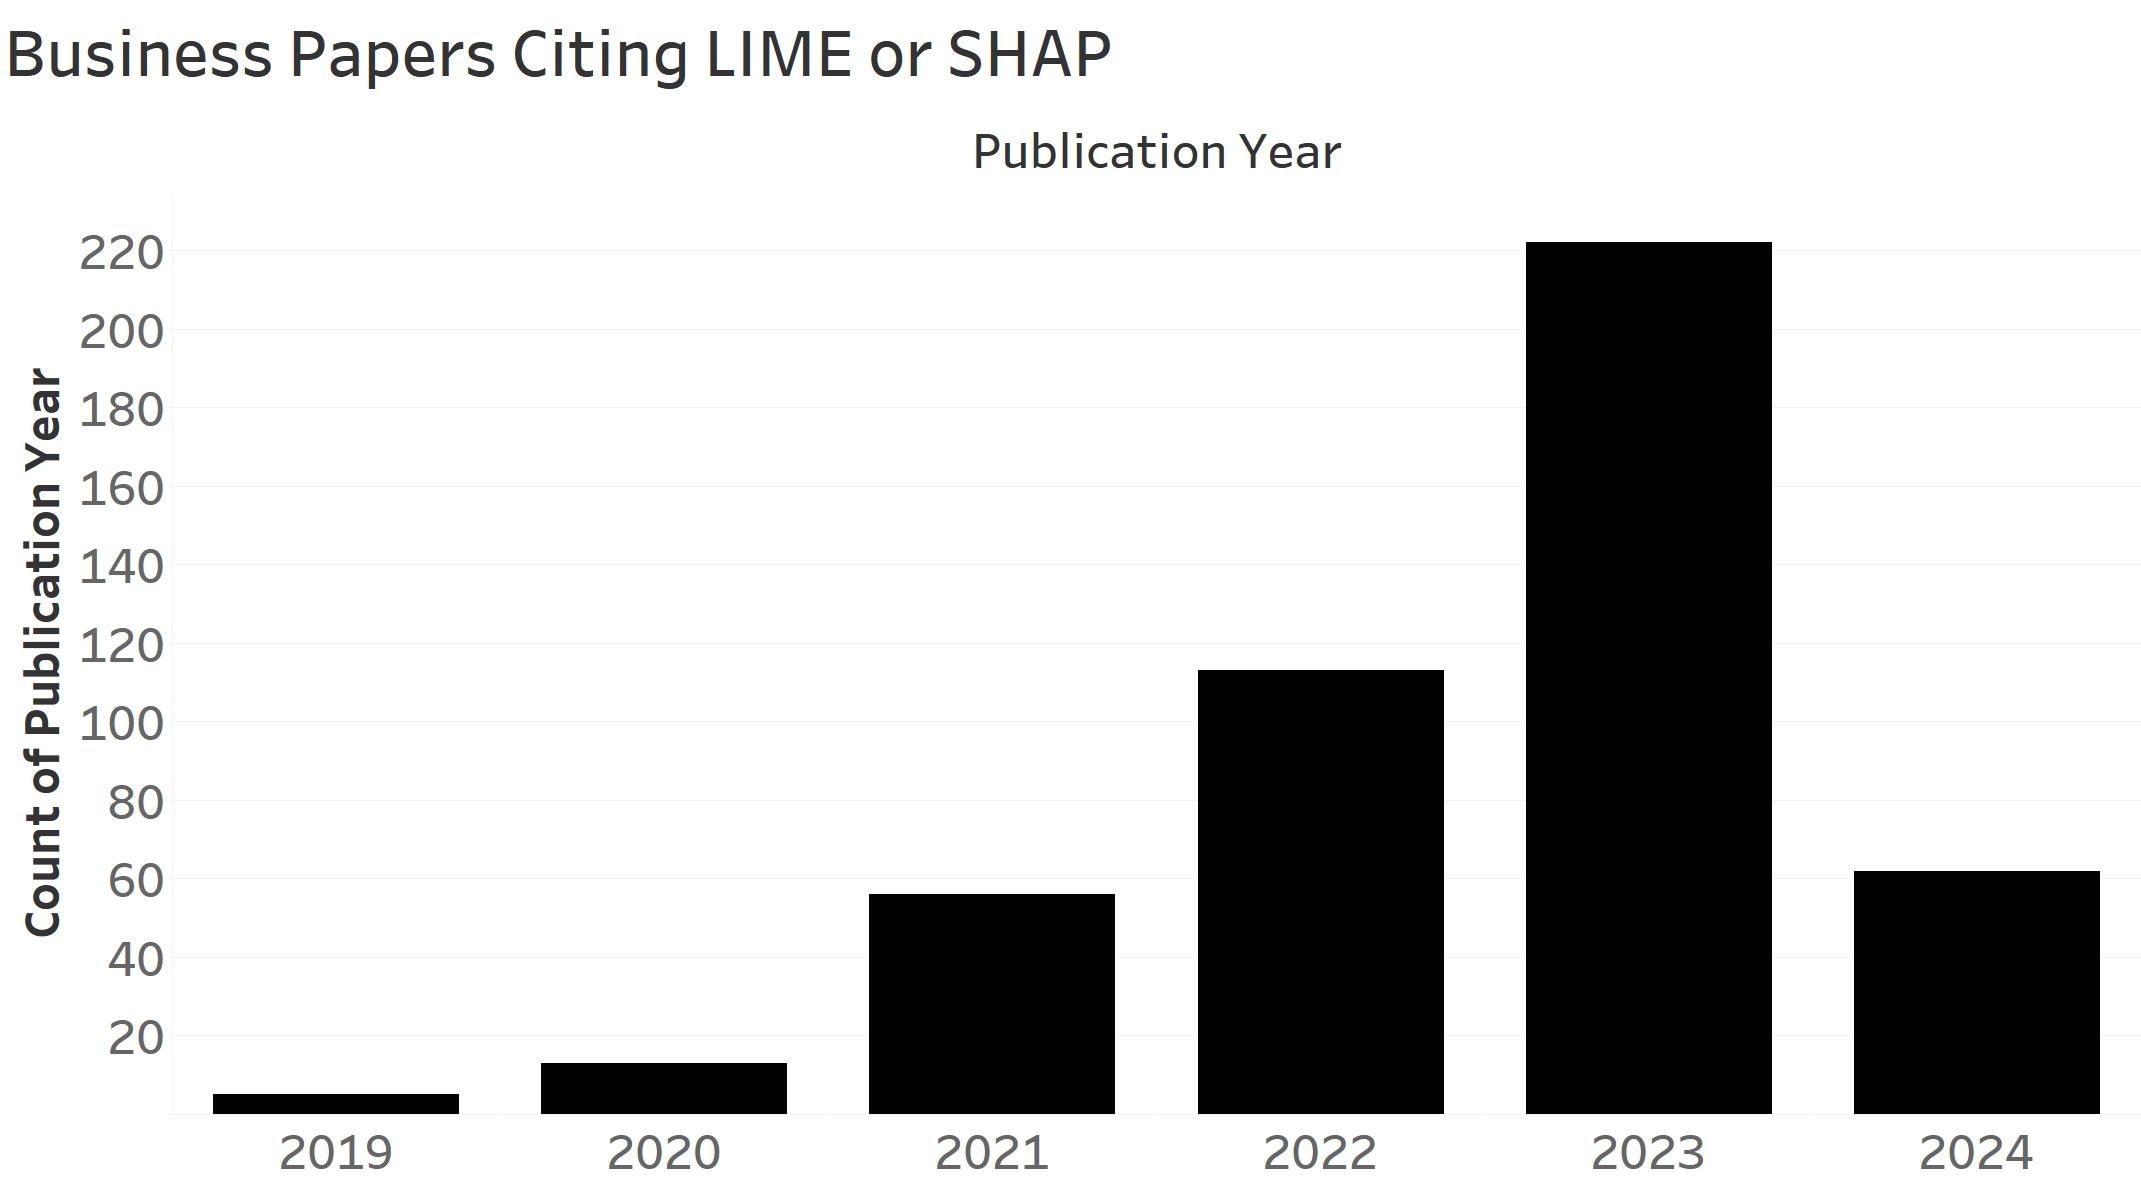
\includegraphics[width=.5\textwidth]{Figs/citations_by_year.png}
            \caption{Year-by-year breakdown of number of papers citing either LIME or SHAP that belong to business-adjacent Web of Science categories.}
            \label{tab:citation_count_graph}
        \end{figure}

        % \begin{figure}
        %     \centering
        %     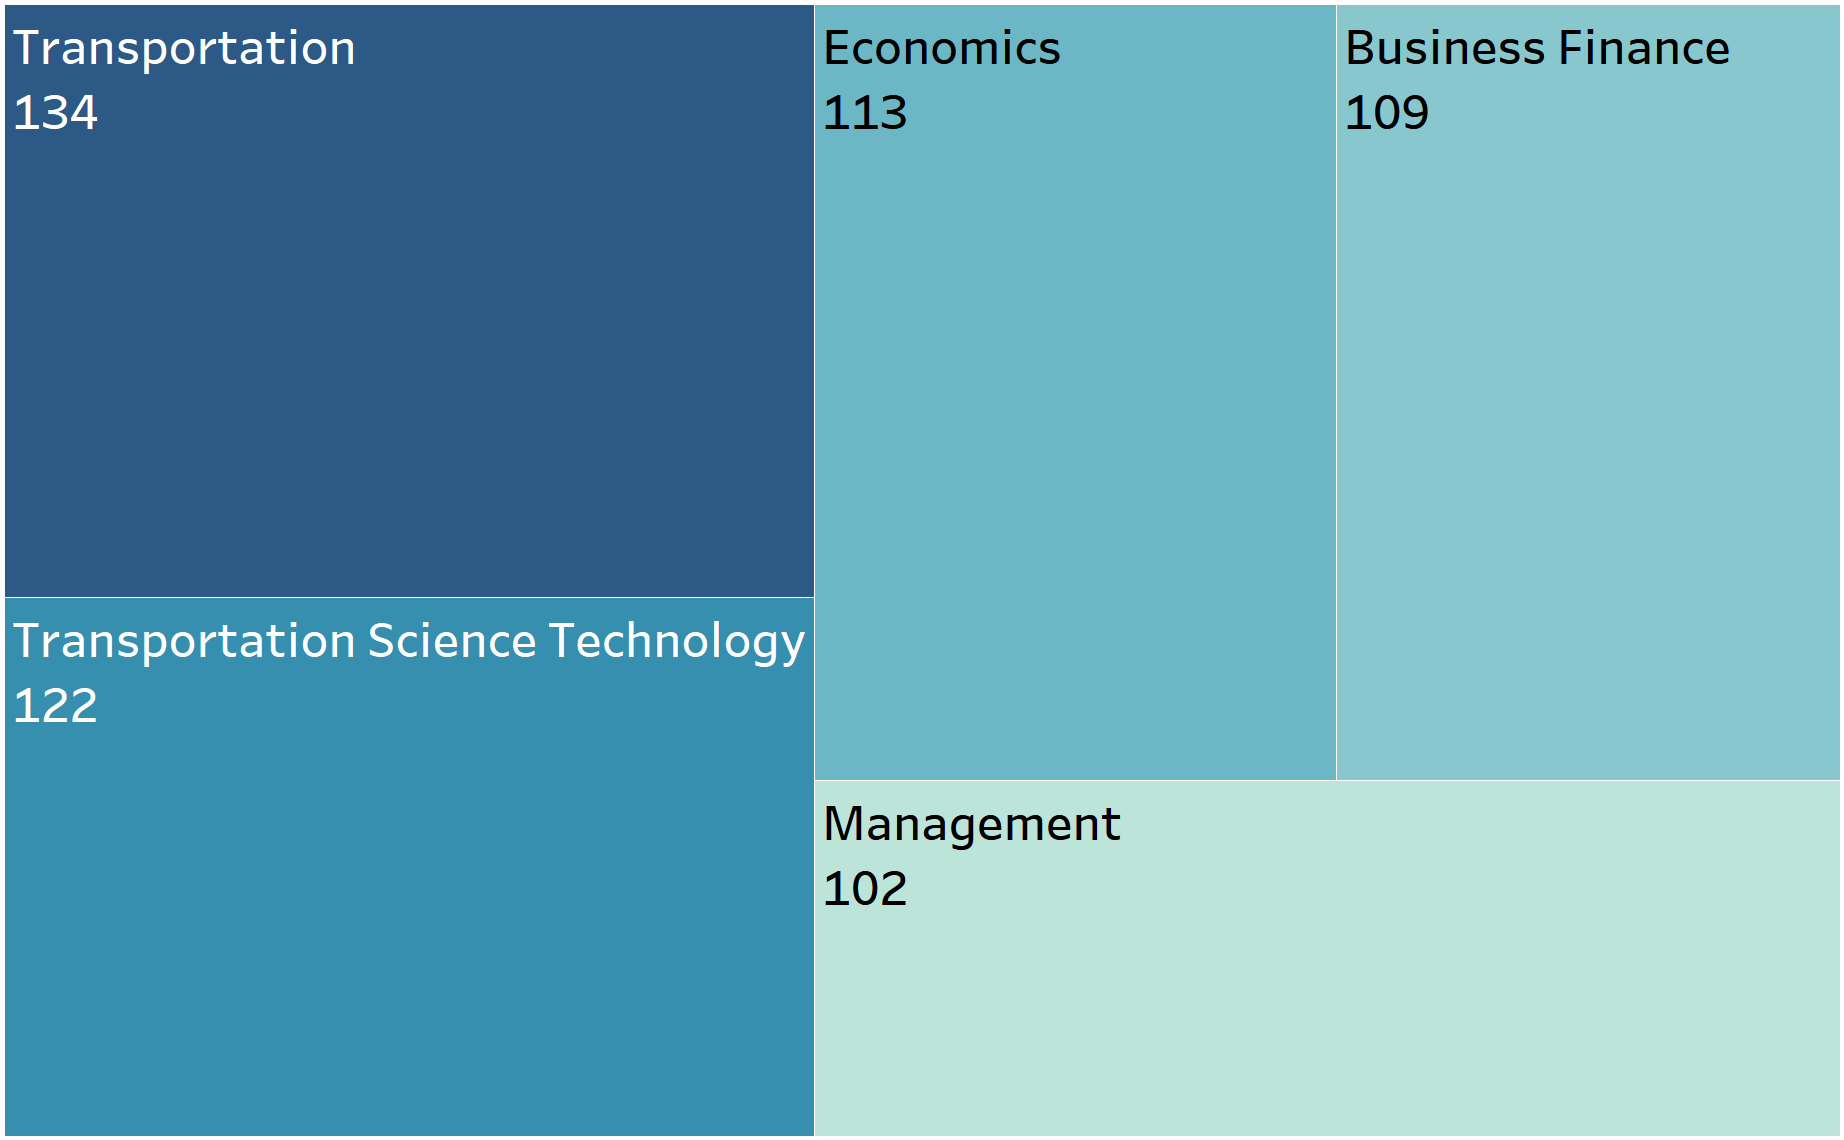
\includegraphics[width=.5\textwidth]{Figs/treemap.png}
        %     \caption{Breakdown of number of papers citing either LIME or SHAP by web of science category.}
        %     \label{tab:treemap}
        % \end{figure}


    % Please add the following required packages to your document preamble:
    % \usepackage{booktabs}
    % \usepackage{lscape}

    % Ambiguous because it's not clear if they mean that the feature is useful for prediction of the target by their model or in reality
    \begin{landscape}
   \begin{table}[htbp] 
    \tiny
    \caption{Types of Language Used when Interpreting Explanations}
    \begin{tabu} to 1\linewidth { | X[l] | X[l] | X[l] | X[l] | X[l] | X[l] |}
       \hline
       \textbf{Language Form} & \textbf{Example 1} & \textbf{Example 2} & \textbf{Example 3}& \textbf{Example 4} & \textbf{Example 5}\\
       \hline
       \textbf{Correct Usage} 
       & However, as outlined in Rudin (2019), the explanations obtained may not be sufficient for a sensitive decision-making process as the results from these methods can be inaccurate representations of the original relationships and potentially misleading. 
       & we analyze feature importance metrics to shed light on how machine learning models arrive at their decisions 
       & We now study the importance of characteristics and their interactions for the performance of gradient boosting and random forests. 
       & To further understand the inner workings of the language-model classifier, we employ Local Interpretable Model-agnostic Explanations 
       & The advantage of this method is that for every prediction the RNN model makes, LIME examines nearby instances and their predictions, and tries to ascertain which parameters have influence over the output using instances in the local environment  \\ \hline 
       \textbf{Extrapolationation}
       & If there are more blue dots with negative SHAP values and more red dots with positive SHAP values, the
values of that feature would be positively correlated with the prediction results. In other words, customers with higher scores for this characteristic are more likely to be churners. 
       & Positive SHAP values indicate that the variable has a facilitative effect on bike-sharing use, while negative values indicate a suppressive effect
       & Here, SHapley Additive exPlanations (SHAP) systematically uncover the crucial elements that govern guest satisfaction during hotel stays.
       & XGBoost, is utilized to capture the quantitative associations, and the SHAP (Shapley Addictive exPlanation) model is used to interpret the results from XGBoost. Our results provide empirical support for prior theoretical findings based on mathematical equilibrium models  
       & Shapley values to understand how various items explain analyst forecasts are generated by utilizing SHAP after XGBoost, when the machine learning model predicts analyst implied ETRs (using the same inputs as predicting actual future ETRs). These Shapley values measure the extent to which various financial
statement items can explain analyst forecasts \\ \hline
       \textbf{Advocacy for Recourse}
       & the method used in this paper has effectively extracted the important influencing variables. On the one hand, it is convenient for investors to quickly evaluate high-polluting enterprises affected by financing, and on the other hand, it can help the government to better promote the transformation of high-polluting enterprises when introducing green credit and green finance
       & When the product contains quad-core (blue), it has a negative impact on customer choices. This relationship implies that a higher spec is recommended for AP in the smartphone
       & Since the number of bus stops, bus lines, bike-sharing trips, parking lots and pedestrian shed ratio have high SHAP importance and substantial effects on metro ridership, relevant last-mile transport facilities should be given sufficient attention by transport planners and operators to enhance these access modes to metro stations.
       & Their SHAP values also raise with the increase of corresponding CV values, revealing that alternative routes with large difference in travel distances, travel speeds or signalized intersection numbers would lead to higher degrees of disequilibrium states at the road network.  
       & The useful forecasting indicators—higher-order moments—used in this study are of great applied economic importance for helping investors, market participants, and policymakers to forecast the volatility of China’s oil futures more effectively, reduce investment risk, and achieve better returns. \\ \hline
       \textbf{Unclear if Assertion Pertains To $\mathcal{M}$ or $\mathcal{G}$}
       &  SHAP can fairly capture the contribution of each predictor and reflect to what extent can each predictor impact the outcome variable
       & But credit and the slope of the yield curve, both domestically and globally are consistently the four most
important predictors. Together, these results strengthen the view that these key variables are robust indicators for predicting financial crises.
       &  According to the feature importance ranking, the top feature may be the potential indicator to trigger financial warning. 
       &  These information can be leveraged by the analyst to understand how to reduce the bankruptcy probability of a specific firm or to get insight in which balance sheet fields need to be improved to increase the rating, therefore providing a business instrument to actively manage clients and structured finance deals. 
       & By analyzing SHAP values, we identify the credit features that significantly influence borrowers' credit scores, gaining insights into the mechanisms behind these features' impact on personal credit scores. \\ \hline
       \textbf{OLS Alternative}
       & Hence, the applied black box algorithm in combination with Shapley values allows to unbox the black box ML approach and provides similar economic insights as provided by pooled OLS
       & we choose to employ machine learning algorithms instead of traditional econometric techniques. The reason is that machine learning offers the following advantages: (1) Machine learning models can deal with non-linearity and complexity...
       %, which allows better modelling of complicated relationships between variables; 
       (2) % Traditional econometric techniques may encounter difficulties when dealing with large datasets due to computational limitations. 
       Machine learning models are often designed to handle large datasets and can be scaled efficiently; (3) Machine learning models can learn from data without the need for explicit model specification. %They can learn patterns and relationships from the data...% and are therefore well suited for cases where the underlying relationships are not well understood and 
       (4) Machine learning models can better capture interaction effects between variables...%, allowing a better understanding of how different factors influence each other. 
       In this way, we then display how key features influence the severity of traffic accidents...% in the early, middle and late stages of the Covid-19 pandemic.
       & To avoid biased estimates and capture non-linear associations, Light Gradient Boosting Machine (LightGBM) model and SHapley additive explanations (SHAP) model are combined to explore the factors affecting the competitiveness of bike-sharing to underground.
       & ...conventional linear HAR models may falter. Additionally, the presence of nonlinearity contributing to volatility forecasting among higher-order moments cannot be identified using conventional linear models. However, machine learning (ML) methods have proven to be effective in addressing multicollinearity and accommodating more sophisticated functional forms, enabling the exploration of complex nonlinear relationships among variables 
       & Machine learning techniques are regarded as a viable alternative to traditional models for traffic forecasting, due to their remarkable ability to capture nonlinearities and exhibit robustness against diverse distributional properties of data. For this reason, machine learning techniques are commonly perceived as a compelling approach for policy and planning analysis \\ \hline
   \end{tabu}
   \label{tab:mistakes}
   \end{table}
   \end{landscape}








   

    
    
    \subsection{Proofs and Experiments}  
        \label{apx_sec:proofs}    
        The proofs for Theorems 1 and 2 in the main paper are provided below, along with simulation experiments that empirically confirm the behavior Theorem 2 predicts about LIME. 
        
        \subsubsection{Proofs}
        \paragraph{Setting of Theorem 1}
            We consider explaining a linear function $f:\mathbb{R}^d \rightarrow \mathbb{R}$ such that $f(\mathbf{x}) = (\boldsymbol{\beta})^T \mathbf{x}$ at the point $\boldsymbol{\xi}\in \mathbb{R}^d$ (which itself was sampled from $\mathcal{N}(0, \mathds{1}_d)$) using a LIME explainer with the following properties. Suppose that LIME samples random vectors $\{\mathbf{x}^{(i)}\}_{i=1}^n$ with $\mathbf{x}^{(i)} \sim \mathcal{N}(\boldsymbol{\xi},\mathds{1}_d)$ for each $n$ and, given a bandwidth parameter $\nu > 0$, weights their distances to $\boldsymbol{\xi}$ using an exponential kernel $\pi(\xi,\mathbf{x}) = exp(-\norm{\boldsymbol{\xi} - \mathbf{x}}_2^2/2\nu^2)$. In the Python LIME implementation, if $\boldsymbol{\xi}$ has feature means $\mu_1,\ldots,\mu_d$ and standard deviations $s_1,\ldots,s_d$, then the samples $\mathbf{x}^{(i)}$ are given by $\sigma_1(z_1 + \mu_1),\ldots,\sigma_D(z_d + \mu_d)$ where each $z_i\sim \mathcal{N}(0,\mathbf{I})$. Since we assumed that $\boldsymbol{\xi} \sim \mathcal{N}(0,\mathbf{I})$, we may assume that each sample is distributed according to $\mathcal{N}(0,\mathbf{I})$ as well. Thus, we may take $\sigma = 1$ in all proofs. 
        
        We assume that LIME follows one of its default settings to solve a ridge regression problem with the following loss function.
        \begin{equation*}
            (\mathbf{y} - \mathbf{X}\mathbf{u})^T \mathbf{W}(\mathbf{y} - \mathbf{X}\mathbf{u}) + (\mathbf{u} - \mathbf{u}_0)^T \Delta(\mathbf{u} - \mathbf{u}_0)
        \end{equation*}
        In this loss function, $\mathbf{X}$ is a data matrix $\mathbf{X} \in \mathbb{R}^{n\times d}$ whose $i^{th}$ row is $\mathbf{x}^{(i)}$ and $\mathbf{W} \in \mathbb{R}^{n\times n}$ is a diagonal weight matrix for each of the $i=1,\ldots,n$ samples with $w_{ii} = \pi(\boldsymbol{\xi},\mathbf{x}^{(i)}) = \exp(-\norm{\boldsymbol{\xi} - \mathbf{x}^{(i)}}_2^2/2\nu^2)$. The response vector $\mathbf{y}\in \mathbb{R}^N$ is defined pointwise by $y^{(i)} = (\boldsymbol{\beta})^T \mathbf{x}^{(i)}$. We set the penalty parameter $\Delta\in \mathbb{R}^{d\times d}$ to $\Delta = \lambda \mathds{I}_{d\times d}$ so that $\Delta$ represents the $L_2$ ridge penalty with hyperparameter $\lambda$. There is another hyperparameter $\mathbf{u}_0 \in \mathbb{R}^d$ which is the target that $\mathbf{u}$ is to be shrunken toward.  We will set $\mathbf{u}_0 = 0$.

        In the proof $i$, and occasionally $i'$, will be used to index the $n$ data samples. $j,k$ and occasionally $l$ will be used to index the $d$ features. Individual data samples in the data matrix $\mathbf{X}$ will be represented with superscript notation, e.g. $\mathbf{x}^{(i)}$. Individual features of a sample will be indexed with subscript notation, e.g. $x^{(i)}_j$. We need not refer to whole rows or columns of $\mathbf{W}$, so it will be indexed entry-wise with $w_{ii}$ for $i=1,\ldots,n$.
    
    
        \paragraph{proof of Theorem 1a}
            The closed form solution to a generalized ridge regression with $\lambda = 1$ and $\mathbf{u}_0 = 0$ is
            \begin{equation*}
                \mathbf{u} = (\mathbf{X}^T \mathbf{W} \mathbf{X} + \mathbf{I})^{-1}(\mathbf{X}^T\mathbf{W}\mathbf{y})% + \Delta \mathbf{u}_0)
            \end{equation*}
                Defining $\hat{\mathbf{\Sigma}}_n = \frac{1}{n}(\mathbf{X}^T \mathbf{W} \mathbf{X} +  \mathbf{I}) \in \mathbb{R}^{d\times d}$ and $\hat{\mathbf{\Gamma}}_n = \frac{1}{n}\mathbf{X}^T \mathbf{W}\mathbf{y}\in \mathbb{R}^{D \times 1}$, we have by the weak law of large numbers that $\hat{\mathbf{\Sigma}}_n$ and  $\hat{\mathbf{\Gamma}}_n$ converge to matrices $\mathbf{\Sigma}=\hat{\mathbf{\Gamma}}_n \mathds{E}[\hat{\mathbf{\Sigma}}_n]$ and $\mathbf{\Gamma}:=\hat{\mathbf{\Gamma}}_n \mathds{E}[\hat{\mathbf{\Gamma}}_n]$ respectively.
                The ridge solution is then denoted $\mathbf{u} := \mathbf{\Sigma}^{-1}\mathbf{\Gamma}$. 
                
                % should actually switch k with i here since i indexes over 1,...,n
                We begin with the computation of $\mathbf{\Sigma}$. We have
                \begin{gather*}
                    \mathbf{\Sigma} = \hat{\mathbf{\Gamma}}_n \frac{1}{n}\mathds{E}[\mathbf{X}^T \mathbf{W} \mathbf{X} + \mathbf{I}] 
                    = \hat{\mathbf{\Gamma}}_n \frac{1}{n}\mathds{E}[\mathbf{X}^T \mathbf{W} \mathbf{X}] + \frac{1}{n} \mathbf{I} \\
                    = \hat{\mathbf{\Gamma}}_n \frac{1}{n}\mathds{E}[\mathbf{X}^T \mathbf{W} \mathbf{X}]
                \end{gather*}
                where expectations are taken over the Wishart distributed random matrices $\mathbf{X}$.
               %  $$           
                Note that $\mathbf{\Gamma} = \frac{1}{n}\mathds{E}[\mathbf{X}^T \mathbf{W} \mathbf{y}]=\frac{1}{n}\mathds{E}[\mathbf{X}^T \mathbf{W} \mathbf{X} \beta]=\frac{1}{n}\mathds{E}[\mathbf{X}^T \mathbf{W} \mathbf{X}] \beta$, so 
                \begin{gather*}
                    \mathbf{\Gamma} = \mathbf{\Sigma} \beta  
                \end{gather*}
        Therefore, we need not actually calculate the expectations or invert $\mathbf{\Sigma}$. It follows that
        \begin{gather*}
            \mathbf{u} = \mathbf{\Sigma}^{-1} \mathbf{\Gamma} \beta = \beta
        \end{gather*}
     
    
        \paragraph{Proof of Lemma 1}
            Let $\mathbf{z} \in \mathbb{R}^N$. First, note that $\mathbf{W}$ induces the norm $\norm{\mathbf{z}}_\mathbf{W} = \sqrt{\mathbf{z}^T \mathbf{W} \mathbf{z}} = \norm{\mathbf{W}^{1/2}\mathbf{z}}_2$. Thus, $\mathbf{X}^T \mathbf{W} \mathbf{X}$ is positive semi-definite. 
            \begin{gather*}
                \mathbf{z}^T \mathbf{X}^T \mathbf{W} \mathbf{X} \mathbf{z} = (\mathbf{X} \mathbf{z})^T \mathbf{W} (\mathbf{X} \mathbf{z}) \\
                = \norm{\mathbf{W}^{1/2} \mathbf{X}\mathbf{z}}_2 \geq 0
            \end{gather*}
            
        \paragraph{Proof of Theorem 1}
            Since the eigenvalues of $\mathbf{A} + \mathbf{I}$ are $\lambda + 1$ for $\lambda$ in the spectrum of $\mathbf{A}$, the eigenvalues of $(\mathbf{A} + \mathbf{I})^{-1}$ have the form $\frac{1}{\lambda + 1}$. By Lemma 1, $\mathbf{A}$ is a symmetric positive semidefinite matrix, and so its singular values coincide with its eigenvalues. $\mathbf{I}$ is positive definite, and the sum of a positive definite matrix and a positive semidefinite matrix is positive definite. Moreover, the inverse of a positive definite matrix is also positive definite.  It follows that the singular values of $(\mathbf{A} + \mathbf{I})^{-1}$ take the form $\frac{1}{\sigma_k(\mathbf{A}) + 1}$ where $\sigma_k(\mathbf{A})$ is the $k^{\text{th}}$ singular value of $\mathbf{A}$. We can now bound $\norm{(\mathbf{A} + \mathbf{I})^{-1}\mathbf{A}}$ in terms of the largest and smallest singular values of $\mathbf{A}$. 
    
            For lower bounds:
            \begin{gather*}
                \norm{(\mathbf{A} + \mathbf{I})^{-1}\mathbf{A}} \geq \sigma_{\min}{(\mathbf{A} + \mathbf{I})^{-1}} \norm{\mathbf{A}} 
                = \frac{\sigma_{\max}(\mathbf{A})}{1 + \sigma_{\max}(\mathbf{A})} %\geq \frac{1}{1 + \sigma_{\max}(\mathbf{A})}
            \end{gather*}
            For upper bounds:
            \begin{gather*}
                \norm{(\mathbf{A} + \mathbf{I})^{-1}\mathbf{A}} \leq \sigma_{\max}{(\mathbf{A} + \mathbf{I})^{-1}} \sigma_{\max}(\mathbf{A}) \\
                \leq \frac{\sigma_{\max}(\mathbf{A})}{\sigma_{\min}(\mathbf{A})+1} \\
                \leq \frac{\sigma_{\max}(\mathbf{A})}{\sigma_{\min}(\mathbf{A})+1}
                \leq \frac{\sigma_{\max}(\mathbf{A})}{\sigma_{\min}(\mathbf{A})} = \kappa(\mathbf{A})
            \end{gather*}
            where $\kappa(\mathbf{A})$ is the condition number of $\mathbf{A}$. 
    
        \paragraph{Proof of Corollary 1}
            As $\nu \rightarrow 0$, $\mathbf{W} \rightarrow \mathbf{0}$, in which case $\mathbf{A}$ converges to $\mathbf{0}$ almost surely and the above bounds have a squeezing effect:
            \begin{equation*}
                0 \leq \norm{(\mathbf{A} + \mathbf{I})^{-1}\mathbf{A}} \leq 0 \implies (\mathbf{A} + \mathbf{I})^{-1}\mathbf{A} = \mathbf{0}
            \end{equation*}
    
    
        \paragraph{Proof of Corollary 2}
            If $\nu \rightarrow \infty$, $\mathbf{W} \rightarrow \mathbf{I}$ and so $\mathbf{A} \rightarrow \mathbf{X}^T \mathbf{X}$ almost surely. Then we have 
            \begin{equation*}
                \frac{\sigma_{\max}(\mathbf{X}^T \mathbf{X})}{\sigma_{\max}(\mathbf{X}^T \mathbf{X})+1} \leq \norm{(\mathbf{A} + \mathbf{I})^{-1}\mathbf{A}} \leq  \kappa(\mathbf{X}^T \mathbf{X})%\frac{\sigma_{\max}(\mathbf{X}^T \mathbf{X})}{\sigma_{\min}(\mathbf{X}^T \mathbf{X})+1} 
            \end{equation*}
            $\mathbf{X}^T \mathbf{X}$ is a Wishart random matrix, so its singular values are on the order of $\sqrt{nd}$. Thus, for $\sqrt{nd} \gg 1$, the lower bound is approximately 1 and the upper bound $\kappa(\mathbf{X}^T \mathbf{X})$ is at most 1 with high probability.  
            %https://arxiv.org/pdf/0810.0800.pdf
            % https://citeseerx.ist.psu.edu/document?repid=rep1&type=pdf&doi=ea7d6ef0f0c530ba591e0833935c4e17fa0794a6 thm3.2
            This can be shown using the following concentration inequality of \citep{edelman2005tails}.
            \begin{equation*}
                \mathds{P}[\kappa(\mathbf{X}^T \mathbf{X}) > 1] \leq c_1 c_2 \leq c_1 (\sqrt{d} + \sqrt{d-1})%\frac{1}{\sqrt{2\pi}} \left(\frac{6}{\mid N - D\mid + 1} \right)^{\mid N-D\mid + 1}
            \end{equation*}
    %https://arxiv.org/pdf/2106.07343.pdf#:~:text=In%20random%20matrix%20theory%2C%20the%20Gordon%E2%80%99s%20theorem%20says,be%20upper%20bounded%20by%20p%20m%2B%20p%20n.
            where $c_1 = \frac{n}{p} \frac{c_{n,d}}{c_{n-1,d+1}}$, $p=\frac{1}{2}(d-n+1)$, $c_{n,d} = \frac{\pi^{3n(n-1)/2}}{2^{nd/2}} \frac{\Gamma(3/2)}{\Gamma_n(3/2)\Gamma_n(p)}$, $\Gamma_n(z) = \pi^{n(n-1)/4} \prod_{i=1}^n \Gamma(z + (i+1)/2)$ is the multivariate gamma function and $c_2$ is the expected value of the largest singular value of a $d-1\times d+1$ matrix of i.i.d. standard Gaussians and the last inequality follows by Gordon's theorem \citep{vershynin2012introduction}.
    
            For fixed $d$, $c_{n,d} \in O\left(\frac{1}{\pi^{n^2} n^2 n!}\right)$. Thus, $c_1 \in O\left(\frac{1}{\pi^{n}n}\right)$. It follows that for sufficiently large $n$, $\mathds{P}[\kappa(\mathbf{X}^T \mathbf{X}) > 1]$ is sufficiently small so that $(\mathbf{A} + \mathbf{I})^{-1}\mathbf{A}$ is squeezed to a value near 1. %CHECK!
    
            
        \paragraph{proof of Theorem 2.}
            This follows immediately from \citep{StrumbeljErik2014Epma} and the assumption that each feature has zero mean.
    
            
        \subsubsection{Insights From Theoretical Results}
            \begin{itemize}
                \item Although explanations using discretized features may be more easily interpretable, they make the explanations less faithful
                \item Users should generally opt to set $n$ to be large 
                \item Users should generally set $\nu$ to be large, otherwise the LIME coefficients may be become zero
                %\item LIME becomes more unfaithful as the number of features $d$ grows. 
                \item The ridge penalty matters only when $\lambda \in O(N)$
            \end{itemize}
    
            \subsubsection{Simulation Experiments}
                \label{sec:simulation_experiments}
                We provide simulations to test the predictions of Theorem 1 and Lemmas 1 and 2 experimentally. In the first simulation we adopt the settings of Theorem 1 and experimentally test the roles of $n$, $\nu$, and $d$ on the convergence of weighted ridge regression using LIME's exponential kernel and the $L_1$ penalty coefficient set to $\Delta=1$. In the second simulation, we use implementation of LIME by its authors and our loan dataset. In this simulation we investigate how the discretization setting affects the actual LIME implementation. In particular, we investigate the ratios $e_{\text{LIME}}(x^{(i)}_j)/\beta_j$. 
    

    
                \paragraph{Role of $\nu$ and $n$ on convergence}
                    We give empirical confirmation of the predictions of Lemmas 1 and 2 in Figure \ref{fig:nu_N_convergence}. To do this, we computed $\norm{\mathbf{H}\mathbf{X} - \mathbf{I}}$ with data matrices $\mathbf{X}$ with $n=100,1000,10000,1000000$ rows  $\mathbf{x}^{(i)} \sim \mathcal{N}(0,\mathbf{I}_4)$ and $\nu=.01,.1,.2,.9,1,.75\sqrt{d},100000$. 
    
                \begin{figure}[ht!]
                \centering
                    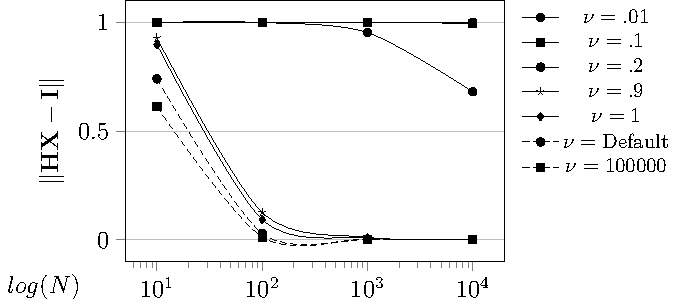
\includegraphics[height=.2\textwidth]{AppendixFigures/apx_lime_conv_nu_N.pdf}%{Figures/fig21.pdf}
                    \caption{Role of $\nu,N$ on $\norm{(\mathbf{X}^T \mathbf{W} \mathbf{X} + \mathbf{I})^{-1}\mathbf{X}^T\mathbf{W}\mathbf{X} - \mathbf{I}}$, with $D=4$}
                    \label{fig:nu_N_convergence}
                \end{figure}

                %\paragraph{Role of $d$ on convergence}
    
                \begin{figure}[ht!]
                \centering
                    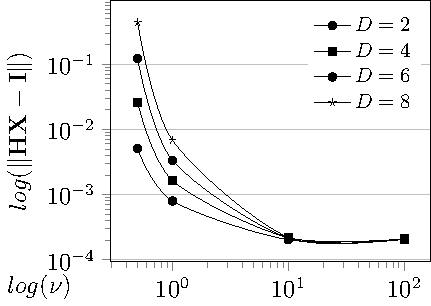
\includegraphics[width=.28\textwidth]{AppendixFigures/apx_lime_conv_D.pdf}%{Figures/fig21.pdf}
                    \caption{Role of $d$ on $\norm{(\mathbf{X}^T \mathbf{W} \mathbf{X} + \mathbf{I})^{-1}\mathbf{X}^T\mathbf{W}\mathbf{X} - \mathbf{I}}$ with $n=50000$}
                    \label{fig:nu_N_convergence}
                \end{figure}
    
                \paragraph{Upper Bounds on $\norm{ (\mathbf{X}^T \mathbf{W} \mathbf{X} + \mathbf{I})^{-1}\mathbf{X}^T\mathbf{W}\mathbf{X}}_2$}
                    We show in Figure \ref{fig:nu_N_convergence} that, except when $\nu$ is too small $\nu=.01$, increasing the number of samples $n$ generally nets a significant decrease in an upper bound for the error of LIME's ridge problem. We use the condition number of  $\norm{ (\mathbf{X}^T \mathbf{W} \mathbf{X} + \mathbf{I})^{-1}\mathbf{X}^T\mathbf{W}\mathbf{X}}_2$ as an upper bound.     
                
                    \begin{figure}[ht!]
                    \centering
                        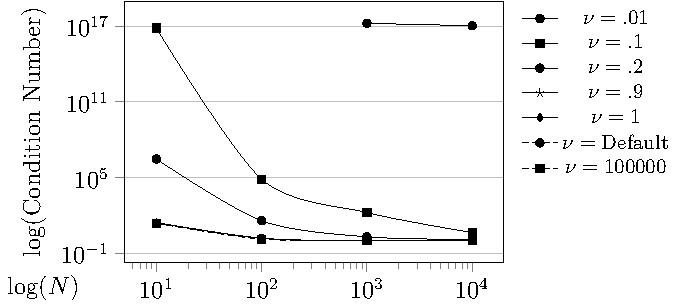
\includegraphics[height=.2\textwidth]{AppendixFigures/apx_lime_conv_cond.pdf}%{Figures/fig21.pdf}
                        \caption{Role of $\nu,N$ on upper bound of $\norm{(\mathbf{X}^T \mathbf{W} \mathbf{X} + \mathbf{I})^{-1}\mathbf{X}^T\mathbf{W}\mathbf{X}}$}
                        \label{fig:nu_N_convergence}
                    \end{figure}
    
                \paragraph{Role of Discretization}
                    We provide evidence of our claim that users should not let LIME discretize numerical features if recovery of the marginal effects is their aim by comparing LIME explainers with and without discretization. For our comparison, we use LIME with and without discretization to explain a linear regressor $f(x) = .05 + .05x_1+ .2x_2+ .8x_3 -.5x_4 +x_5$ with $x_i \sim \mathcal{N}(0,1)$ for all $i$. $\nu$ is set to the default value. We pick 100 test set instances and explain each two sets of 100 LIME explainers. The first set of LIME explainers do not use feature discretization while the second set does. The $i^{th}$ explainer has its random seed set to $n$ in both sets. For each set of explainers, we plot the ratios $C_i:= e(x_j)_i/\beta_i$ for $i=1,\ldots,5$ in Figure \ref{fig:c_demo}.

                %As we claimed in Section 3, the LIME explainers with no feature discretization generally have $C_i$ closer to $1$ than the LIME explainers with discretization. The difference is especially stark with $C_{1}$, which is always 1 with no discretization and between -10 and 20 with discretization. Note that when $C_i$ is negative, LIME has misidenified how feature $i$ impacts the output of $f$. Moreover, in accordance with Theorem 1 and \citep{garreau20theoretical}, we see that $C_i$ can differ significantly across $i$, indicating that $e(x_j)$ is not directly proportional to $\boldsymbol{\beta}$ regardless of whether discretization is used. 

                We show the empirical distributions of proportionality constants $C_j$ for both LIME explainers in Figure \ref{fig:c_demo}. The most striking result is that all $C_j$ are centered around $\frac{1}{3}$ and contained in $[-1,1]$ when discretization is turned off, but $C_1$ takes on values in $[-10,10]$ with a mean of $\sim 3.70$ and $C_2,C_3,C_4,C_5$ have respective means of $.52$, $.06$, $.03$, and $-.001$ when discretization is allowed. Thus, when discretization is allowed, LIME may distort the $\beta_j$ more and have severe inconsistency between how much distortion is present across each $j$.
                
                %use fbox to tailor crop
                \begin{figure}[ht!]
                \centering
                    \begin{subfigure}{.28\textwidth}
                    \centering
                    %\fbox{\includegraphics[width=\textwidth,trim=0 10 70 70 mm, clip=true]{Figures/fig21.pdf}}%{Final_Figures/fig20.png}
                    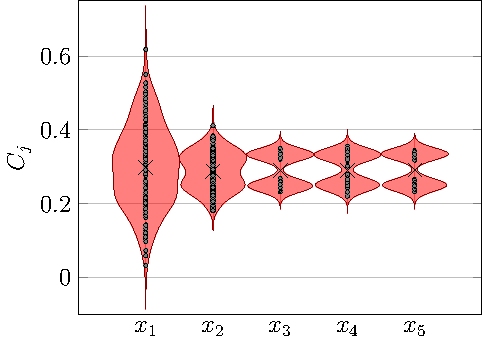
\includegraphics[width=\textwidth]{AppendixFigures/apx_lime_proportionality-figure0.pdf}%{Figures/fig21.pdf}
                    \caption{No discretization}
                    \label{fig:empirical_c}
                    \end{subfigure}%
                    \hspace{3cm}
                    \begin{subfigure}{.28\textwidth}
                    \centering
                    %\fbox{\includegraphics[width=\textwidth,trim=0 10 70 70 mm, clip=true]{Figures/fig21.pdf}}%{Final_Figures/fig20.png}
                    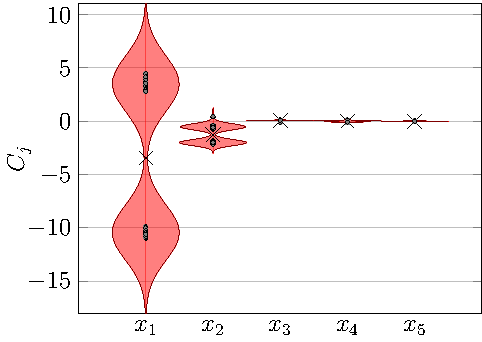
\includegraphics[width=\textwidth]{AppendixFigures/apx_lime_proportionality-figure1.pdf}%{Figures/fig21.pdf}
                    \caption{Discretization allowed}
                    \label{fig:theoretical_cs}
                    \end{subfigure}%
                \caption{Empirical $C_j$ for 100 applicants from 100 LIMEs with/without discretization, and all other parameters set to the defaults.}
                \label{fig:c_demo}
                \end{figure}
    

    


    
    
  
    
    
    \subsection{Details and Additional Experiments for Section \ref{sec:causes_of_misalignment}}
        \label{apx_sec:misalignment_exp_details}
        This section provides details about how the datasets were generated in Section \ref{sec:causes_of_misalignment}.
        %as well as additional experiments that show how correlation and confounding can affect interpretations of post hoc explanations. Table \ref{tab:simulated_variations} documents what features are used in each experiment. 
    
            % \begin{table}[]
            % % determine target width of combined cols 2 and 3:
            % \settowidth\mylenA{Correlated \\ Features} 
            % % determine usable width of cols 2 and 3:
            % \setlength\mylenB{(\mylenA-3\tabcolsep)/3}
            % \centering
            % \begin{tabular}{|c|*{3}{wc{\mylenB}|}*{3}{wc{\mylenB}|}*{3}{wc{\mylenB}|}}
            % \hline
            % \textbf{Experiment} & \multicolumn{3}{c|}{\makecell{\textbf{Correlated} \\ \textbf{Features}}} & \multicolumn{3}{c|}{\makecell{\textbf{Unobserved} \\ \textbf{Confounder}}} & \multicolumn{3}{c|}{\makecell{\textbf{Observed} \\  \textbf{Confounder}}} \\ \hline
            % \textbf{Feature} & \textbf{$\mathcal{G^*}$} & \textbf{$\mathcal{G_{\text{effect}}}$} & \textbf{$\mathcal{M}$}             
            % &   \textbf{$P_1$} & \textbf{$\mathcal{G_{\text{effect}}}$} & \textbf{$\mathcal{M}$}              & \textbf{$P_1$} & \textbf{$\mathcal{G_{\text{effect}}}$}             & \textbf{$\mathcal{M}$}             \\ \hline
            % Age              & \checkmark& \textcolor{red}{\checkmark}    & \checkmark                                                            & \checkmark  & \checkmark    & \checkmark                               & \checkmark& \checkmark   & \checkmark                               \\ \hline
            % Sex              & \checkmark& \checkmark & \checkmark   & \checkmark  & \checkmark   & \checkmark                                & \checkmark& \checkmark & \checkmark                                 \\ \hline
            % Inquiries        & \checkmark& \checkmark  & \checkmark &  \checkmark     &\multicolumn{1}{c|}{\checkmark}        & \checkmark & \checkmark & \textcolor{red}{\checkmark}    & \checkmark                     \\ \hline
            % Cosigner         & \checkmark& \checkmark   & \checkmark                                                              & \checkmark  & \checkmark                                   & \checkmark& \checkmark & \checkmark  &\multicolumn{1}{c|}{\checkmark}                                \\ \hline
            % Utilization      & \checkmark& \checkmark  & \checkmark                                                                 & \checkmark  & \checkmark   & \checkmark                                & \checkmark& \textcolor{red}{\checkmark}  & \checkmark                                \\ \hline
            % Credit Score     & \checkmark& \textcolor{red}{\checkmark} & \checkmark                                 &                               & \checkmark  & \checkmark  & \checkmark & \textcolor{red}{\checkmark}  & \checkmark                                \\ \hline
            % %Social Support   & \multicolumn{1}{c|}{}    & \multicolumn{1}{c|}{}                               &                                    &  \multicolumn{1}{c|}{}  & \multicolumn{1}{c|}{\textcolor{red}{\checkmark}} & \multicolumn{1}{c|}{} & \multicolumn{1}{c|}{}                                 &\multicolumn{1}{c|}{}             &\multicolumn{1}{c|}{}                      \\ \hline
            % Income & \multicolumn{1}{c|}{}    & \multicolumn{1}{c|}{}      &     & \multicolumn{1}{c|}{}                                       & \multicolumn{1}{c|}{\textcolor{red}{\checkmark}} & \multicolumn{1}{c|}{} & \multicolumn{1}{c|}{}                                  &\multicolumn{1}{c|}{}  &\multicolumn{1}{c|}{}                                 \\ \hline
            % \end{tabular}
            % \caption{Table indicating whether the ground truth models $P_1$ and $\mathcal{G}_{\text{effect}}$ use each feature  and whether $\mathcal{M}$ has access to each feature in data produced by ground truth models using them in each experiment. Features which are correlated in $\mathcal{G}_{\text{effect}}$ are marked red.} 
            % \label{tab:simulated_variations}
            % \end{table}
            
        \subsubsection{Correlated Features}
            % We have $\mu_\text{Credit Score}=550$, $\sigma_\text{Credit Score}=20$, $\mu_\text{Age}=38$, $\sigma_\text{Age}=13$, and $\rho=.8$. 
            % \begin{equation*}
            %     \begin{bmatrix}
            %         \text{Credit Score} \\
            %         \text{Age}
            %     \end{bmatrix}
            %     \sim 
            %     \mathcal{N}\left(            
            %     \begin{bmatrix}
            %         \mu_\text{Credit Score} \\
            %         \mu_\text{Age}
            %     \end{bmatrix},             \begin{bmatrix}
            %         \sigma_\text{Credit Score}^2,\ \sigma_\text{Credit Score} \sigma_\text{Age} \rho \\
            %         \sigma_\text{Age} \sigma_\text{Credit Score} \rho,\ \sigma_\text{Age}^2  \\
            %     \end{bmatrix}
            %     \right)
            % \end{equation*}
    
        
            % To isolate the individual data-related effects in each experiment, we will create an ideal data generator $P_1$ together with a data generator $\mathcal{G}_{\text{effect}}$ symptomatic of each effect. $P_1$ generates data such that all features are pairwise independent, observed, and unconfounded.
        
            % We then compare the abilities of SHAP and LIME to explain models $\mathcal{M}$ trained on data generated by $P_1$ and $\mathcal{G}_{\text{effect}}$ for each effect. Following the experimental setup of Section \ref{sec:misalignment}, each experiment will be represented by a plot of the metric of interest for that experiment computed using SHAP and LIME explanations of models $\mathcal{M}$ trained on 100 applicants from the test sets of data given by both $P_1$ and $\mathcal{G}_{\text{effect}}$.  At the end of this section, we also investigate the desirable situation where SHAP and LIME explain an MLP model $\mathcal{M}$ with reasonable accuracy trained on the data from $P_1$ to demonstrate that explanations of $\mathcal{M}$ are still imperfect even if the data has no correlated or confounded features. 
    
            % In this section, the model data generators $P_1$ use a simplified set of features. Namely, age, sex, credit inquiries, credit utilization, credit score, and availability of a cosigner. All features are independent of each other. When training the models $\mathcal{M}$ on $P_1$ and $\mathcal{G}_{\text{effect}}$, we have the setup where 5000 applicants are generated and $\mathcal{M}$ is an MLP with ROC AUC at least .85. Table \ref{tab:simulated_variations} illustrates which features are used as inputs to each ground truth model $P_1$ and $\mathcal{G}_{\text{effect}}$, as well as which features are involved in the effect in $\mathcal{G}_{\text{effect}}$ that breaks the causal inference conditions. It also marks when $\mathcal{M}$ has access to a feature in training data provided by ground truth model using that feature.
        
            %With enough observations, you will eventually be able to identify the separate effects of even highly collinear (but never perfectly collinear) variables. This is why Rob Franzese and UMich likes to call multicollinearity "micronumerosity."
        
            Figure \ref{fig:marital_sign_accs} shows bar plots of the sign accuracies for the marital status feature by SHAP and LIME before and after making the cosigner feature depend on marital status. The bar plots show that the addition of dependencies between features is associated with a loss of the ability to give ``married" the correct sign for both SHAP and LIME. Additionally, Figure \ref{fig:marital_rank_diff} shows the distributions of the absolute differences between the given and correct rank for ``married" before and after addition of correlated features. We see that for both SHAP and LIME, the average ranking error for ``married" is much smaller when the features are mutually independent than otherwise. 
            \begin{figure}[ht!]
                \centering
                \begin{subfigure}{.28\textwidth}
                  \centering
                  \captionsetup{justification=centering}
                  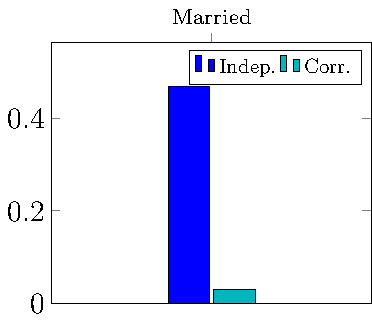
\includegraphics[width=\textwidth]{Figs/apx_marital-figure1.pdf}%{Figures/fig_age_col.pdf}%{Figures/lime_spearman_colinear.png}
                                %\includegraphics[width=.9\linewidth]{Figures/lime_shap_Spearman_magnitude.png}
    
                  \caption{SHAP}%Spearman rank correlations of ranked feature importance magnitudes from LIME against the true ranked magnitudes from $\mathcal{G}$.}
                   \label{fig:marital_sign_accs_shap}
                \end{subfigure}%
                \hspace{3cm}
                \begin{subfigure}{.28\textwidth}
                  \centering
                     \captionsetup{justification=centering}
                  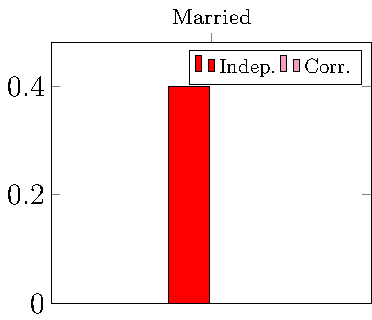
\includegraphics[width=\textwidth]{Figs/apx_marital-figure0.pdf}%{Figures/fig_score_col.pdf}%{Figures/shap_spearman_colinear.png}
    
                  %\includegraphics[width=.9\linewidth]{Final_Figures/fig9b.png}%{Figures/shap_spearman_colinear.png}
                  \caption{LIME}%Spearman rank correlations of signed feature importance magnitudes from SHAP and LIME against the true ranking from $\mathcal{G}$.}
                   \label{fig:marital_sign_accs_lime}
                \end{subfigure}
                
                \caption{Bar charts showing how SHAP and LIME (almost) never can correctly identify the sign of the marital status feature when it is used to determine the cosigner feature.}%rankings of age and credit score change from when being independent to when credit score becomes a function of age}
                \label{fig:marital_sign_accs}
            \end{figure}

            \begin{figure}[ht!]
                \centering
                \begin{subfigure}{.28\textwidth}
                  \centering
                  \captionsetup{justification=centering}
                  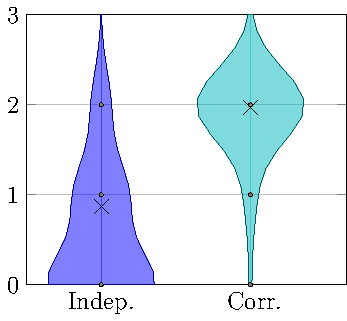
\includegraphics[width=\textwidth]{Figs/apx_marital-figure2.pdf}%{Figures/fig_age_col.pdf}%{Figures/lime_spearman_colinear.png}
                                %\includegraphics[width=.9\linewidth]{Figures/lime_shap_Spearman_magnitude.png}
    
                  \caption{SHAP}%Spearman rank correlations of ranked feature importance magnitudes from LIME against the true ranked magnitudes from $\mathcal{G}$.}
                   \label{fig:marital_rank_diff_shap}
                \end{subfigure}%
                \hspace{3cm}
                \begin{subfigure}{.28\textwidth}
                  \centering
                     \captionsetup{justification=centering}
                  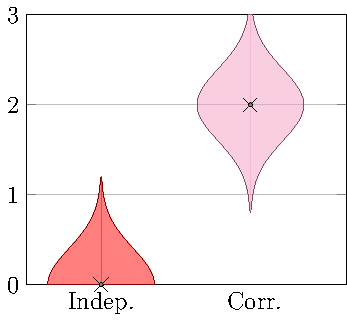
\includegraphics[width=\textwidth]{Figs/apx_marital-figure3.pdf}%{Figures/fig_score_col.pdf}%{Figures/shap_spearman_colinear.png}
    
                  %\includegraphics[width=.9\linewidth]{Final_Figures/fig9b.png}%{Figures/shap_spearman_colinear.png}
                  \caption{LIME}%Spearman rank correlations of signed feature importance magnitudes from SHAP and LIME against the true ranking from $\mathcal{G}$.}
                   \label{fig:marital_rank_diff_lime}
                \end{subfigure}
                
                \caption{Violin plots showing the differences between the given rank and true rank of marital status depending on whether marital status influences possession of a cosigner. Lower is better.}%rankings of age and credit score change from when being independent to when credit score becomes a function of age}
                \label{fig:marital_rank_diff}
            \end{figure}


    
    \subsubsection{Pervasiveness of Data-Misalignment}
        Full details for the experimental design used in Section 5.2.3 follow. We synthesize 100 datasets with randomly selected numbers of features between 3 and 100, and randomly selected numbers of rows between 100 and 10000. The features are i.i.d. according to $\mathcal{N}(0,5)$. The target of each dataset is binary and is produced using randomly generated linear decision boundaries with coefficients between -10 and 10. Additionally, we vary the amount of label noise in each dataset by fixing a probability $p \in [0,.1]$ before generating the dataset and then flipping each label with probability $p$. We split the dataset into 80\% training data and 20\% testing data.

        We generate a model for each dataset using the Python AutoML package auto-sklearn \citep{feurer-neurips15a}. We do not allow the AutoML to perform feature pre-processing. We set the AutoML to search among the following model types: MLP, XGBoost, Decision Tree, ExtraTrees, Random Forest, and \textcolor{red}{\ldots}. The models are evaluated using 5-fold cross validation with respect to test set accuracy. We run the AutoML in a parellelized fashion with 16 cores and allow a maximum of 10 minutes to produce a model for each dataset. 

        Since the number of features differs across the datasets, we report the results for our three metrics in the following fashion, conditioned on the number of features. For directionality, for each $d$, we report the mean directionality for the actual most important feature over 100 test set instances from the datasets with dimension $d$. Similarly, we report the feature-wise mean directionality and the percentage of features whose directionality was under $.5$. We also report the mean concordance and mean relevance for $k=3$ in the same fashion.

        % \begin{figure}[t!]
        %     \subfloat[SHAP Top-1 Directionality]{%
        %         \raisebox{0cm}{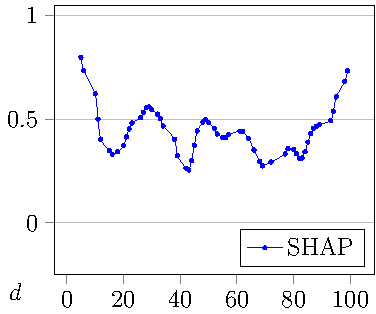
\includegraphics[width=.28\textwidth]{Figs/synthetic-figure0.pdf}}%
        %         \label{apx_fig:shap_vary_d_accs}%
        %     }\hspace{1cm}%\hfill
        %     \subfloat[SHAP Mean Directionality]{%
        %         \raisebox{0cm}{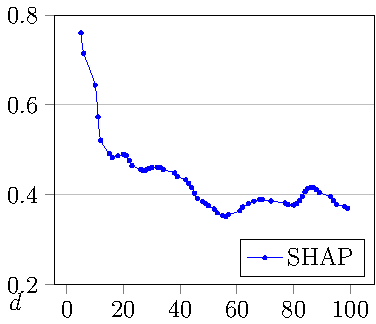
\includegraphics[width=.28\textwidth]{Figs/synthetic-figure2.pdf}}%
        %         \label{apx_fig:shap_vary_d_spearmans}%
        %     }\hspace{1cm}%\hfill
        %     \subfloat[SHAP \% Features With Directionality $<.5$]{%
        %         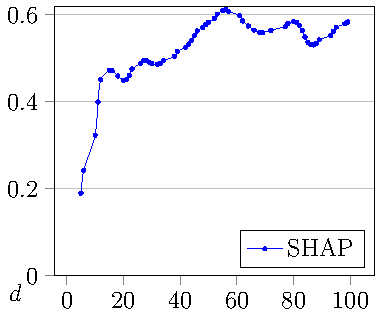
\includegraphics[width=.28\textwidth]{Figs/synthetic-figure4.pdf}%
        %         \label{apx_fig:shap_vary_d_recalls}%
        %     }\\
        %     \subfloat[LIME Top-1 Directionality]{%
        %         \raisebox{0cm}{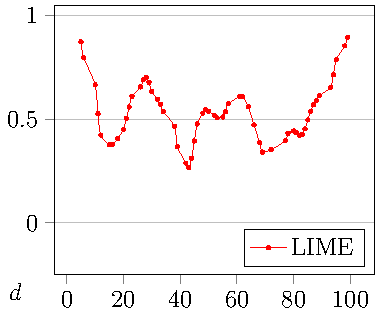
\includegraphics[width=.28\textwidth]{Figs/synthetic-figure1.pdf}}%
        %         \label{apx_fig:lime_vary_d_accs}%
        %     }\hspace{1cm}%\hfill
        %     \subfloat[LIME Mean Directionality]{%
        %         \raisebox{0cm}{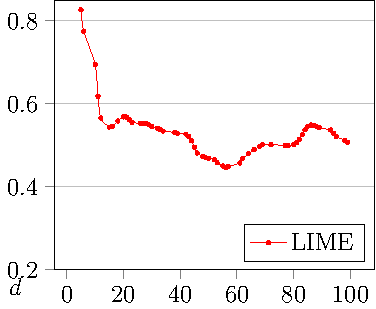
\includegraphics[width=.28\textwidth]{Figs/synthetic-figure3.pdf}}%
        %         \label{apx_fig:lime_vary_d_spearmans}%
        %     }\hspace{1cm}%\hfill
        %     \subfloat[LIME \% Features with Directionality $<.5$]{%
        %         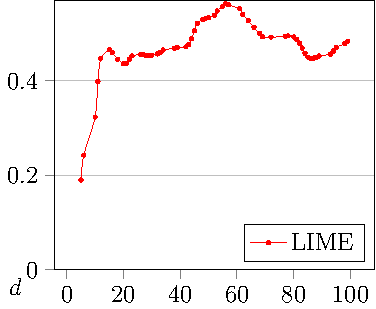
\includegraphics[width=.28\textwidth]{Figs/synthetic-figure5.pdf}%
        %         \label{apx_fig:lime_vary_d_recalls}%
        %     }\\
        %     \caption{Relationship of number of features $d$ with top-1 directionality, feature-wise mean directionality, and the percentage of features with directionality $<.5$}
        %     \label{fig:lime_shap_vary_d}
        % \end{figure}



        % \begin{figure}[t!]
        %     \centering
        %     \subfloat[SHAP Concordance]{%
        %         \raisebox{0cm}{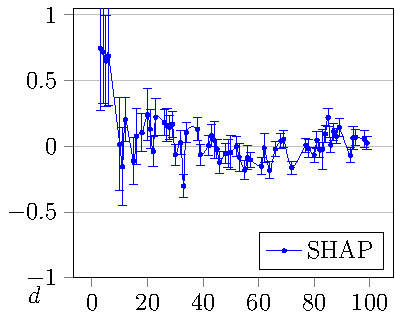
\includegraphics[width=.28\textwidth]{Figs/synthetic-figure6.pdf}}%
        %         \label{fig:shap_vary_d_accs}%
        %     }\hspace{1cm}%\hfill
        %     \subfloat[SHAP Top-3 Relevance]{%
        %         \raisebox{.05cm}{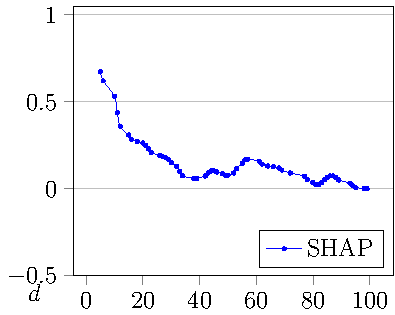
\includegraphics[width=.28\textwidth]{Figs/synthetic-figure8.pdf}}%
        %         \label{fig:shap_vary_d_spearmans}%
        %     }\\
        %     \subfloat[LIME Concordance]{%
        %         \raisebox{0cm}{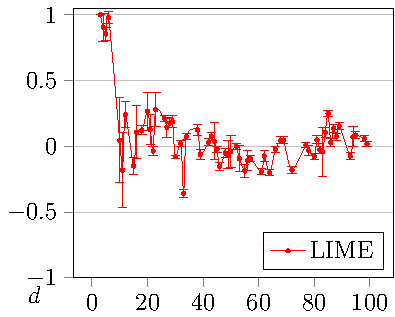
\includegraphics[width=.28\textwidth]{Figs/synthetic-figure7.pdf}}%
        %         \label{fig:lime_vary_d_accs}%
        %     }\hspace{1cm}%\hfill
        %     \subfloat[LIME Top-3 Relevance]{%
        %         \raisebox{0cm}{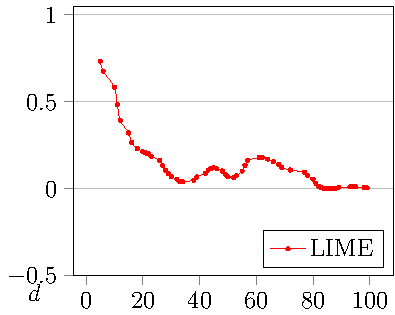
\includegraphics[width=.28\textwidth]{Figs/synthetic-figure9.pdf}}%
        %         \label{fig:lime_vary_d_spearmans}%
        %     }\\
        %     \caption{Relationship of number of features $d$ with concordance, and relevance of top 3 features}
        %     \label{fig:lime_shap_vary_d}
        % \end{figure}



        % \begin{figure}[t!]
        %     \subfloat[SHAP Directionality]{%
        %         \raisebox{.2cm}{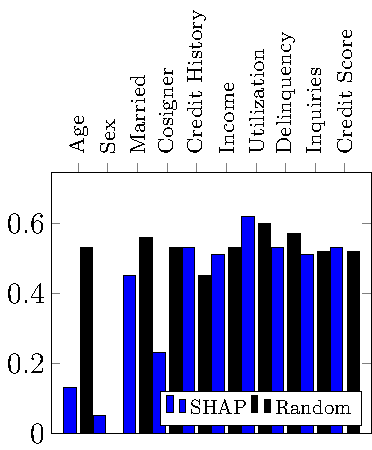
\includegraphics[width=.28\textwidth]{Figs/sec4_1_split-figure0.pdf}}%
        %         \label{subfig:mlp_avg_shap_sign_accs}%
        %     }\hspace{1cm}
        %     \subfloat[SHAP Concordance]{%
        %          \raisebox{.05cm}{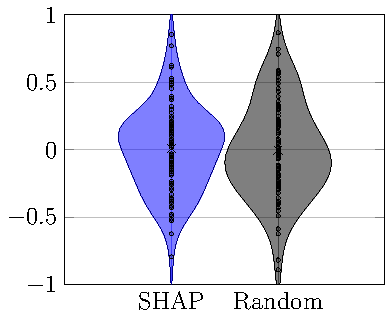
\includegraphics[width=.28\textwidth]{Figs/sec4_1_split-figure2.pdf}}%
        %         \label{subfig:mlp_auc_shap_spearmans}%
        %     }\hspace{1cm}
        %     \subfloat[SHAP Relevance]{%
        %         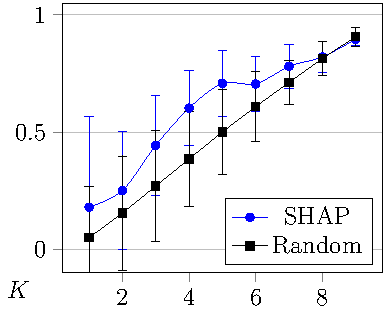
\includegraphics[width=.28\textwidth]{Figs/sec4_1_split-figure4.pdf}%
        %         \label{subfig:mlp_auc_shap_recalls}%
        %     }\\
        %     \subfloat[LIME Directionality]{%
        %         \raisebox{.2cm}{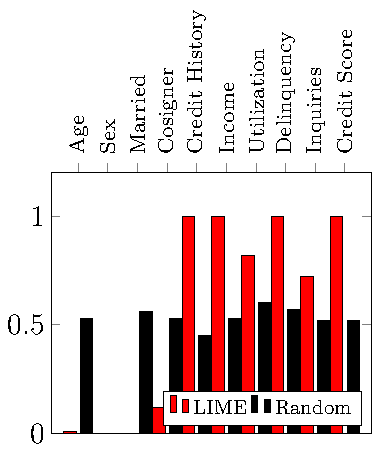
\includegraphics[width=.28\textwidth]{Figs/sec4_1_split-figure1.pdf}}%
        %         \label{subfig:mlp_auc_lime_sign_accs}%
        %     }\hspace{1cm}%\hfill
        %     \subfloat[LIME Concordance]{%
        %         \raisebox{.05cm}{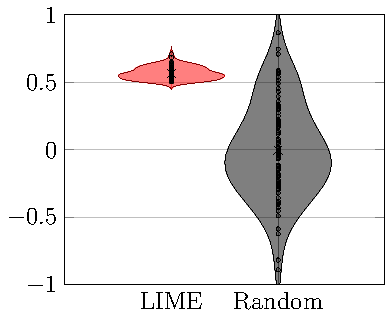
\includegraphics[width=.28\textwidth]{Figs/sec4_1_split-figure3.pdf}}%
        %         \label{subfig:mlp_auc_lime_spearmans}%
        %     }\hspace{1cm}
        %     \subfloat[LIME Relevance]{%
        %         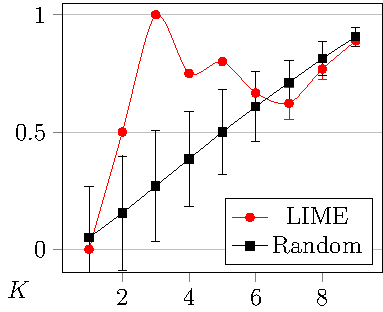
\includegraphics[width=.28\textwidth]{Figs/sec4_1_split-figure5.pdf}%
        %         \label{subfig:mlp_auc_lime_recalls}%
        %     }\\
        %     \caption{Comparisons of results for our three metrics for SHAP, LIME, and an explainer that gives random feature importance values}
        %     \label{fig:mlp_auc_increase}
        % \end{figure}

    

     
    
    
   

    
    

    \subsection{Details and  Experiments Related to Inconsistency}
        \label{apx_sec:inconsistency}
        In this section, we provide a more thorough analysis of the phenomenon of explainer inconsistency. We begin by discussing how the large number of unique mappings from $X$ to $Y$ in ML models' search spaces leads to an even larger number of potential explanations for phenomena regarding $X\rightarrow Y$. Then we investigate how, even if one fixes an ML model $\mathcal{M}$, there are many potential explanations for each prediction $\mathcal{M}(\boldsymbol{\xi})$ because of inconsistency between distinct explainer models and within the same explainer model. Finally, we demonstrate the problem of instability, where, fixing a model and explainer, explanations of the model's predictions on two similar inputs are very dissimilar. 
        
        \subsubsection{Prediction Stage Issues: Diversity of Decision Boundaries for $\mathcal{M}$}
            \label{sec:rashomon_overfitting}
            Because SHAP and LIME aim to approximate the local behavior of $\mathcal{M}$, their explanations are governed by $\mathcal{M}$'s decision boundary \citep{han22which}. This entails that explanations for the same prediction task differ across both model classes and across unique members of each model class. For example, explanations of decision trees and neural networks differ because decision trees partition the data space into rectangular regions while neural networks can partition the data space into irregularly shaped regions. Furthermore, two decision trees with different splits will partition the data into different rectangular regions. 
    
            % consider mentioning bootstrap
            Additionally, because models $\mathcal{M}$ are trained to achieve good predictive performance on given input data, the training data also affects explanations. Different pre-processing methodologies change the representation of the mapping from the features to the target that $\mathcal{M}$ aims to approximate, and therefore affects explanations by e.g. changing the meaning of feature importance. Also, measurement error and bias in the dataset limit how faithful $\mathcal{M}$ can be to the underlying true $\mathcal{G}$ and hence limit how much information about the marginal effects can be extracted. 
            
            %The inconsistency of explanations is, furthermore, related to the diversity of decision boundaries in two senses of the word diversity. First, different models necessarily have different decision boundaries. Second, the volatility of a decision boundary contributes to explanation instability.
    
    
            % put this first per dr. wang's request
            % talk about model performance and rashomon mayble?
            \paragraph{\textbf{Inconsistency from  Choices for $\mathcal{M}$}}
            Despite being trained on the same data and attaining approximately the same predictive performance, explanations of two distinct models with different decision boundaries will necessarily be different. Note that two unique decision boundaries could be obtained for the same dataset by the same class of models, e.g. by training two decision trees with differing maximum tree depths. Figure \ref{box} demonstrated how different explanations of two models from different classes can be by showing that SHAP's explanations for why the same applicant was approved by MLP and XGBoost models were both misaligned and in different ways. Thus, different pipelines using different models tend to yield different explanations, none of which are necessarily representative of the actual marginal effects.
    
            % DOUBLE CHECK THE SHAP RESULT
            We illustrate the problem of inconsistency in greater generality by checking how often  feature importance signs and feature rankings of $m=100$ applicants agree when produced by combinations of the following models $\mathcal{M}$ and explainers $\mathcal{E}$. We consider three models with ROC AUC at least $.9$, an MLP $\mathcal{M}_{\text{MLP}}$, and two distinct XGBoost models $\mathcal{M}_{\text{XGB1}}$ and $\mathcal{M}_{\text{XGB2}}$. We consider two explainers, $\mathcal{E}_{\text{LIME}}$ and $\mathcal{E}_{\text{SHAP}}$.
            
            
            We showcase inconsistency between models from different model classes by investigating the agreement between the explanations produced by $(\mathcal{M}_{\text{MLP}}, \mathcal{E}_{\text{LIME}})$ and $(\mathcal{M}_{\text{XGB1}}, \mathcal{E}_{\text{LIME}})$ as well as those between $(\mathcal{M}_{\text{MLP}}, \mathcal{E}_{\text{SHAP}})$ and $(\mathcal{M}_{\text{XGB1}}, \mathcal{E}_{\text{SHAP}})$. Figure \ref{fig:mlp_xgb_corr} shows that credit score was the only feature which consistently got the same feature importance sign. Also, on average, rankings from explanations of the MLP and XGBoost were nearly uncorrelated for both SHAP and LIME. Since researchers should not, therefore, expect to get the same insights about marginal effects from explanations of models from two different model classes, the choice of what model to explain becomes an issue without a clear solution.
            % SHAP and LIME explanations of two pairs of models, all with AUC$\simeq .85$. The first pair consists of one MLP and one XGBoost, while the second pair consists of two distinct XGBoost models. Figure \ref{fig:model_corrs} presents the results for both pairs. 
            
            Next, we showcase that there is also inconsistency between explanations of models from the same class by considering explanations between   $(\mathcal{M}_{\text{XGB1}}, \mathcal{E}_{\text{LIME}})$ and $(\mathcal{M}_{\text{XGB2}}, \mathcal{E}_{\text{LIME}})$ as well as those between $(\mathcal{M}_{\text{XGB1}}, \mathcal{E}_{\text{SHAP}})$ and $(\mathcal{M}_{\text{XGB2}}, \mathcal{E}_{\text{SHAP}})$, where XGB1 and XGB2 are XGBoost models which are made distinct by changing the random seed used for initialization in their otherwise identical training routine. Figure \ref{fig:xgb_xgb_corr} shows that SHAP had perfect agreement in all explanations while LIME was very inconsistent. SHAP's feature importance signs were completely consistent, while LIME's were only consistent for credit score. The mean concordance for SHAP is about 1 and the mean correlation for LIME is low, just above .25. The reason SHAP's explanations are perfectly consistent is because, when explaining the XGBoost models, all features except for credit score and income are always given Shapley values of 0. 
            The results from Figures \ref{fig:mlp_xgb_incon} and \ref{fig:xgb_xgb_incon} therefore suggest that there is usually disagreement in the feature rankings obtained by explaining two different models, but perhaps not when SHAP is explaining two models of the same type. 
            
            % \begin{figure}[ht!]
            % \centering
            %     \begin{subfigure}[t]{0.28\textwidth}
            %     \centering
            %     \captionsetup{width=1.6\linewidth}
            %     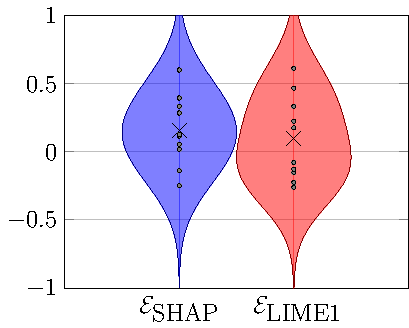
\includegraphics[width=\textwidth]{Figs/sec5_2_incon-figure0.pdf}
            %     \caption{Correlation between pairs of explanations of an MLP and XGBoost model} \label{fig:mlp_xgb_corr}
            % \end{subfigure}
            % \hspace{2cm}
            % \begin{subfigure}[t]{0.28\textwidth}
            %     \centering
            %     \captionsetup{width=1.6\linewidth}
            %     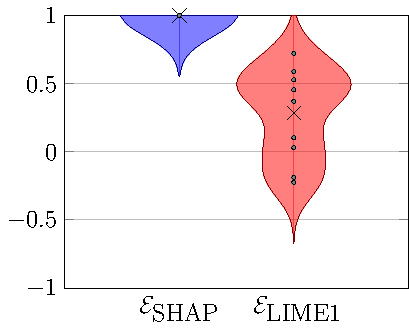
\includegraphics[width=\textwidth]{Figs/sec5_2_incon-figure1.pdf}
            %     \caption{Correlation between pairs of explanations from two distinct XGBoost models} 
            %     \label{fig:xgb_xgb_corr}
            % \end{subfigure}
            % \caption{Violin plots of Spearman correlations between pairs of explanations of different combinations of black box models}
            % \label{fig:model_corrs}
            % \end{figure}
    
            \begin{figure}[ht!]
            \centering
            \begin{subfigure}[t]{0.28\textwidth}
                \centering
                %\captionsetup{width=1.6\linewidth}
                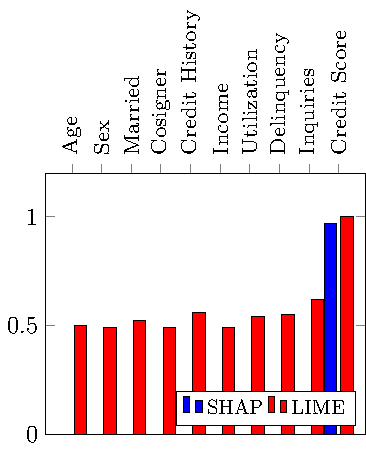
\includegraphics[width=\textwidth]{Figs/sec5_2_incon-figure4.pdf}
                \caption{Sign Agreement} 
                \label{fig:mlp_xgb_sgn}
            \end{subfigure}
            \hspace{2cm}
                \begin{subfigure}[t]{0.28\textwidth}
                \centering
                %\captionsetup{width=1.6\linewidth}
                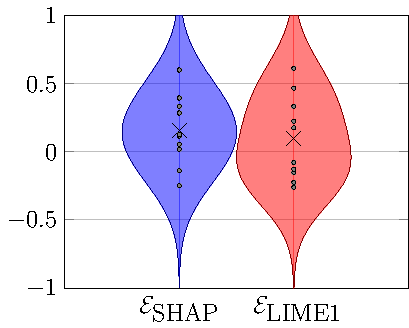
\includegraphics[width=\textwidth]{Figs/sec5_2_incon-figure0.pdf}
                \caption{Correlation} \label{fig:mlp_xgb_corr}
            \end{subfigure}
            \caption{Agreement between pairs of explanations of an MLP and XGBoost model}
            \label{fig:mlp_xgb_incon}
            \end{figure}
    
            \begin{figure}[ht!]
            \centering
            \begin{subfigure}[t]{0.28\textwidth}
                \centering
                %\captionsetup{width=1.6\linewidth}
                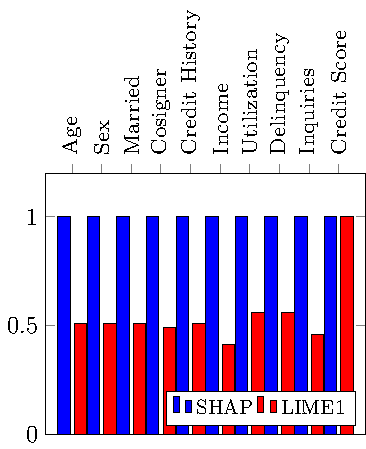
\includegraphics[width=\textwidth]{Figs/sec5_2_incon-figure6.pdf}
                \caption{Sign Agreement} 
                \label{fig:xgb_xgb_sgn}
            \end{subfigure}
                \begin{subfigure}[t]{0.28\textwidth}
                \centering
                %\captionsetup{width=1.6\linewidth}
                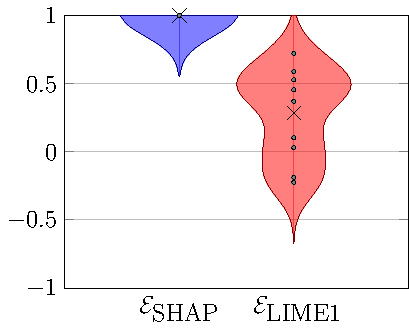
\includegraphics[width=\textwidth]{Figs/sec5_2_incon-figure1.pdf}
                \caption{Correlation} \label{fig:xgb_xgb_corr}
            \end{subfigure}
            \caption{Agreement between pairs of explanations from two distinct XGBoost models}
            \label{fig:xgb_xgb_incon}
            \end{figure}
    
    
            % instability moved to appendix
            %
            
            % \paragraph{\textbf{Inconsistency from Data pre-processing Methodology}}
            %     We identify two ways data pre-processing can affect post hoc explanations. First, the pre-processing affects the decision boundaries of models trained on it, which we know from Section \ref{sec:causes_of_misalignment} affects explanations. Second, pre-processing routines like standardization can change the signs of feature values, which we know from Section \ref{sec:theoretical_considerations} can cause the Shapley value sign to differ from that of $\boldsymbol{\beta}$. 
    
            %     To test this, we constructed two models $\mathcal{M}$ and $\mathcal{M}_{\text{Std.}}$ that were trained on the same dataset without and with feature standardization, respectively. $\mathcal{M}_{\text{Std.}}$ has associated pairs of explainers $\mathcal{E}_{\text{LIME Std.}}$ and $\mathcal{E}_{\text{SHAP Std.}}$. Similarly, $\mathcal{M}$ has associated pairs of explainers $\mathcal{E}_{\text{LIME}}$ and $\mathcal{E}_{\text{SHAP}}$.
                
                
            %     We then compared $(\mathcal{M}_{\text{Std.}}, \mathcal{E}_{\text{LIME Std.}})$ and $(\mathcal{M}_{\text{Std.}}, \mathcal{E}_{\text{SHAP Std.}})$ with explanations from pipelines pipelines $(\mathcal{M}, \mathcal{E}_{\text{LIME}})$ and $(\mathcal{M}, \mathcal{E}_{\text{SHAP}})$, respectively. It is evident from our results, shown in Figure \ref{fig:lime_shap_preproc_corr}, that neither SHAP nor LIME were robust to data normalization. SHAP's relatively worse sensitivity to data standardization can be explained by Equation \ref{eqn:shap_gt}, since the SHAP value of a feature depends linearly on both the value and mean of that feature. 
        
            %     \begin{figure}[ht!]
            %         \centering
            %         %\begin{subfigure}{.3\textwidth}
            %           \centering
            %           \captionsetup{justification=centering}
            %           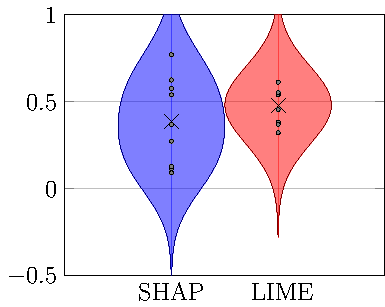
\includegraphics[width=.28\textwidth]{Figs/apx_preproc-figure3.pdf}
            %           \caption{Correlations between feature rankings from explanation of model trained on standardized data with feature rankings from explanations of model trained on data with no standardization}%Spearman rank correlations of ranked feature importance magnitudes from LIME against the true ranked magnitudes from $\mathcal{G}$.}
            %            %\label{fig:lime_income}
            %         %\end{subfigure}%
            %         %\caption{}%Violin plots of feature importance values for \emph{income} from SHAP and LIME for cases when \emph{income} is unconfounded and confounded by the unobserved social support feature}
            %         \label{fig:lime_shap_preproc_corr}
            %     \end{figure}
    
        
        
    
    
        
        
        \subsubsection{Explanation Stage Issues: Inconsistency Between and Within Explainers}
            \label{sec:conflict_between_within}
                %To motivate the use of multiple post hoc explainers, we show that they may explain the same outcome in different ways with differing degrees of accuracy. 
                Inconsistency also comes from the explanation stage since
                different explanations can be obtained by different explainers, or the same explainer method with different hyperparameters.
                We will demonstrate this by showing that not only do SHAP and LIME disagree in their explanations, but two distinct LIME explainers can also disagree. In view of Theorems 1 and 2, unmodified explanations from SHAP and LIME should not agree, so we compare LIME explanations with normalized SHAP explanations. 
                
                % move to discussion
                %\citep{visani21stability}, for example, studied the theoretical side of the issue by showing that LIME explanations are statistically not repeatable under identical conditions of explanation generation. \citep{kommiya21towards} showed that feature rankings from LIME, SHAP, and counterfactual explainers are often uncorrelated (especially with large data dimensions). \citep{Krishna2022TheDP} studied the practical side of the issue and showed (from interviews) that practitioners given multiple explanations from multiple explainers are forced to make confusing and somewhat arbitrary choices of what explanation to keep.
                    To test how consistent SHAP and LIME are with each other, we use both explainers to explain the same set of predictions by the same machine learning model XGB1 which we defined in the previous section and compare the results. For each of the $i=1,\ldots,m$ instances $\mathbf{x}^{(i)}$ we compute the sign agreement and rank correlation between the pair of explanations $e_\text{SHAP}(\mathbf{x}^{(i)})$ and $e_\text{LIME}(\mathbf{x}^{(i)})$. The results of our experiment, illustrated in Figure \ref{fig:lime_shap_incon}, show that the SHAP and LIME explanations of XGB1 are not consistent with each other. There is no substantial agreement in feature importance sign for any feature except or credit score (recall that SHAP assigns all features but credit score and income 0 importance when explaining XGB1). Unsurprisingly, the mean rank correlation between the pairs of explanations is close to 0, indicating that SHAP and LIME generally disagree in their rankings. It is worth noting that the level of disagreement would be \emph{worse} if we did not normalize the SHAP values. 
                    
                
                    
    % new experiment
    % signs feature importance values
    % Fig 1 a: pick one instance, run LIME 10 times with different seeds, and show a bar plot for the percentages of positive values and negative values for the most important feature. （pick a good example - percentages are very different, 90% vs 10% -- low entropy)
    % Fig 1 b: pick one instance, run LIME 10 times with different seeds, and show a bar plot for the percentages of positive values and negative values for the most important feature. (pick a bad example - percentages are very similar, 50% vs 50% -- high entropy)
    % Fig 1 c: for the above experiment, compute the entropy of that two percentages (smaller the better), repeat the experiment on 100 instances and plot a violinplot
    % ranking of feature importance
    % Fig 2 a & b: pick one instance, run LIME 10 times with different seeds, show the distribution (histogram) of ranking for two features.
    % Fig 2 c: for a given instance, run LIME 10 times with different seeds, each time getting a ranking of feature importance. Out of the total 10 rankings, do a pairwise comparison, which produces 45 pairs of Spearman rank correlation. Repeat on 100 instances. violinplot the 45 * 100 Spearman rank correlation.
    
    
    
        %        
    In addition to different types of explainers disagreeing with each other, it is unfortunately also the case that individual explainers of the same type can produce a set of explanations for the same input that has some internal disagreement. We demonstrate this phenomenon with LIME only because SHAP is deterministic. %%The points generated in the sampling step are determined by random seed, the number of samples to generate around the point to explain, the kernel function (default Gaussian), and the kernel width defining the size of the neighborhood around the point to explain. 
                % i used signed feature importance vals here
               We constructed two unique LIME explainers $\mathcal{E}_{\text{LIME1}}$ and $\mathcal{E}_{\text{LIME2}}$ and computed the concordance between explanations from $(\mathcal{M}_{\text{XGB1}}, \mathcal{E}_{\text{LIME1}})$ and $(\mathcal{M}_{\text{XGB1}}, \mathcal{E}_{\text{LIME2}})$ and plotted the results in Figure \ref{fig:lime_corrs}. The first explainer had default hyperparameter settings and the second used a smaller kernel width. Since most of the violin area in Figure \ref{fig:lime_lime_xgb_corr} is below 1, this means that the two LIME explainers disagreed on almost every explanation. The nature of the disagreement was such that the pairs of explanations consistently assigned different signs to all features except for cosigner. Researchers may reasonably anticipate that repeated uses LIME to explain the same prediction will give different results and make selecting which explanation(s) to use in their study challenging. 
    
      
    % \begin{figure}[ht!]
    % \centering
    %     \begin{subfigure}[t]{0.28\textwidth}
    %     \centering
    %     \captionsetup{width=1.6\linewidth,justification=centering}
    %     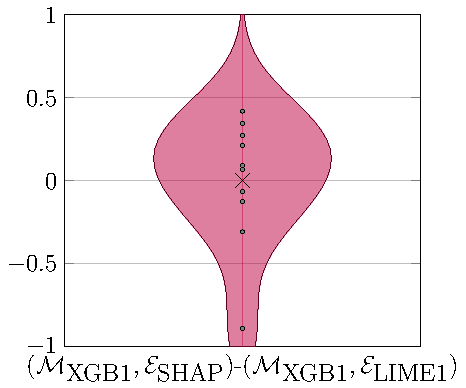
\includegraphics[width=\textwidth]{Figs/sec5_2_incon-figure2.pdf}
    %     \caption{Correlation between SHAP and LIME explanations of pairs of explanations the same XGBoost model} \label{fig:lime_shap_xgb_corr}
    % \end{subfigure}
    % \hspace{2cm}
    % \begin{subfigure}[t]{0.28\textwidth}
    %     \centering
    %     \captionsetup{width=1.6\linewidth,justification=centering}
    %     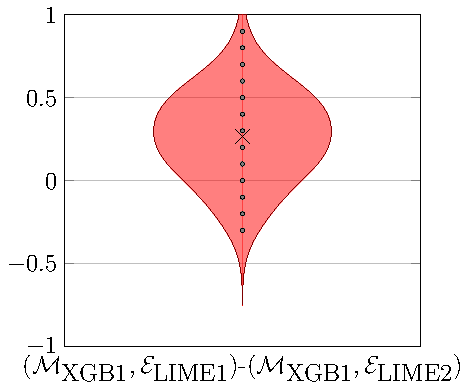
\includegraphics[width=\textwidth]{Figs/sec5_2_incon-figure3.pdf}
    %     \caption{Correlation between pairs of explanations of the same XGBoost model from two distinct LIME explainers} \label{fig:lime_lime_xgb_corr}
    % \end{subfigure}
    % \caption{Violin plots of rank correlations between pairs of explanations of one XGBoost model from different combinations of explainers}
    % \label{fig:explainer_corrs}
    % \end{figure}
    \begin{figure}[ht!]
    \centering
    \begin{subfigure}[t]{0.28\textwidth}
        \centering
        %\captionsetup{width=1.6\linewidth,justification=centering}
        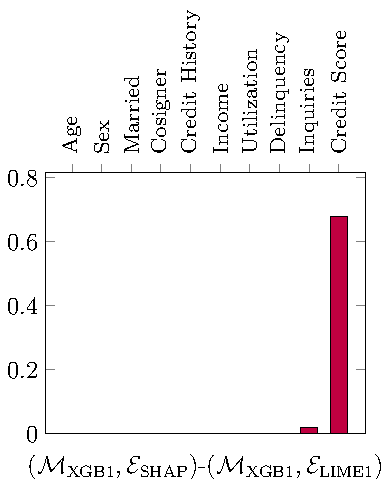
\includegraphics[width=\textwidth]{Figs/sec5_2_incon-figure7.pdf}
        \caption{Sign agreement}
        \label{fig:lime_shap_xgb_sgn}
    \end{subfigure}
    \hspace{2cm}
        \begin{subfigure}[t]{0.28\textwidth}
        \centering
        %\captionsetup{width=1.6\linewidth,justification=centering}
        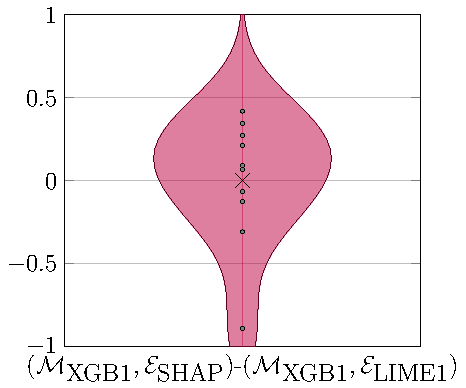
\includegraphics[width=\textwidth]{Figs/sec5_2_incon-figure2.pdf}
        \caption{Correlation} \label{fig:lime_shap_xgb_corr}
    \end{subfigure}
    \caption{Agreement between pairs of explanations of the same XGBoost model from SHAP and LIME}
    \label{fig:lime_shap_incon}
    \end{figure}
    
    \begin{figure}[ht!]
    \centering
    \begin{subfigure}[t]{0.28\textwidth}
        \centering
        %\captionsetup{width=1.6\linewidth,justification=centering}
        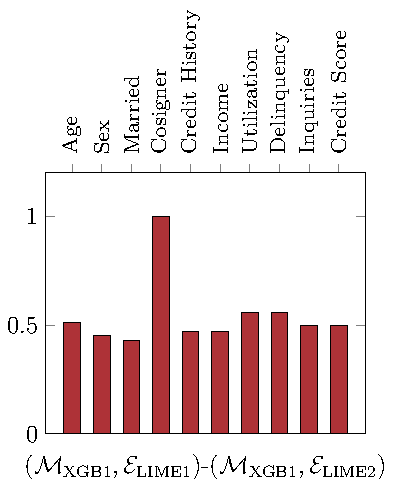
\includegraphics[width=\textwidth]{Figs/sec5_2_incon-figure8.pdf}
        \caption{Sign agreement} 
        \label{fig:lime_lime_xgb_sgn}
    \end{subfigure}
    \hspace{2cm}
    \begin{subfigure}[t]{0.28\textwidth}
        \centering
        %\captionsetup{width=1.6\linewidth,justification=centering}
        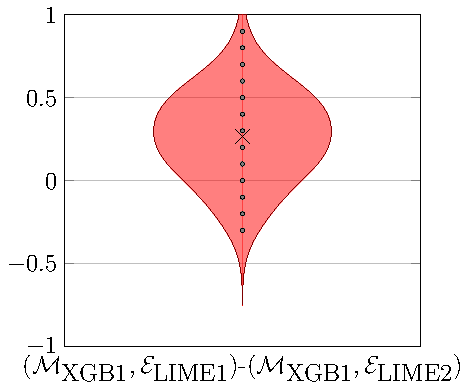
\includegraphics[width=\textwidth]{Figs/sec5_2_incon-figure3.pdf}
        \caption{Correlation } 
        \label{fig:lime_lime_xgb_corr}
    \end{subfigure}
    \caption{Agreement between pairs of explanations of the same XGBoost model from two distinct LIME explainers}
    \label{fig:lime_corrs}
    \end{figure}
        
        % % EXPOUND
         
         
    
    %---------------------------------
    
    
            
            The second goal of this section is to introduce instability, another kind of inconsistency. 
            
        
        \subsubsection{Instability Due to Decision Boundary Volatility}         
            \label{sec:instability}
            Intuitively, explanations for the outcomes occurring in similar scenarios should be similar as well. In fact, the reasoning behind the decisions made on applicants with sufficiently similar profiles should be identical. Otherwise, applicants could have reason to suspect unfairness. But consider a situation where inputs $\boldsymbol{\xi}^{(1)}$ and $\boldsymbol{\xi}^{(2)}$ are nearby but $\mathcal{M}(\boldsymbol{\xi}^{(1)})$ and $\mathcal{M}(\boldsymbol{\xi}^{(2)})$ are distant. If one only cares about the faithfulness of the explainer with respect to $\mathcal{M}$, the explanations of $\boldsymbol{\xi}^{(1)}$ and $\boldsymbol{\xi}^{(2)}$ should definitely be dissimilar. However, if we care about faithfulness with respect to $\mathcal{G}$, and $\mathcal{G}(\boldsymbol{\xi}^{(1)})$ and $\mathcal{G}(\boldsymbol{\xi}^{(2)})$ are close, instability is not desirable. Instability is therefore a problem when an explainer is too unstable due to, e.g., overfitting. Both when $\mathcal{M}$ overfits $\mathcal{G}$ and when $\mathcal{E}$ overfits $\mathcal{M}$ can cause unnecessary variability to be captured by $\mathcal{E}$ and result in unnecessary instability. 
          
            To demonstrate instability, we construct a two-dimensional loan approval model based only on income and credit utilization and check the instability of LIME's coefficients when overfitting is and is not present. %Our approach for evaluating stability is similar to the coefficient stability index (CSI) from \citep{visani21stability}. 
            The first step of the experiment is to generate a dataset using a ground truth model $\mathcal{G}$ which decides approval using a linear combination of income and credit utilization. Then we train an MLP $\mathcal{M}_1$ on a noisy version of that dataset where some points near the decision boundary of $\mathcal{G}$ have their label flipped. $\mathcal{M}_1$ misclassifies those noise points and is therefore meant to represent a classifier that did not overfit by fitting the noise points correctly. We construct another MLP $\mathcal{M}_{2}$ which does overfit the noisy data and consequently has a comparatively erratic decision boundary. The decision boundaries of $\mathcal{M}_1$ and $\mathcal{M}_2$ are shown in Figure \ref{fig:dbds}. Finally, we quantify coefficient stability by computing the Euclidean distances between the LIME coefficients for pairs of LIME explanations of points near the decision boundary of $\mathcal{M}_1$ and their nearest neighbor with the same label. 

            Figure \ref{fig:dbd_dists} shows that explainers for $\mathcal{M}_{2}$ are more unstable than those for $\mathcal{M}_1$. This is evident because the distances between the coefficient sets of LIME explainers for pairs of nearby points are always much higher for LIME explainers of $\mathcal{M}_{2}$ than for explainers of $\mathcal{M}_1$.% When explaining $\mathcal{M}$, the mean distance is $9e-4$ and the standard deviation is $1e-3$, while when explaining $\mathcal{M}_{\text{overfit}}$, the mean distance is $2e-2$ and the standard deviation is $1.7e-2$. Explainers of $\mathcal{M}$ have high coefficient stability because the distances are concentrated near 0 in Figure \ref{fig:dbd_dists}. Explainers of $\mathcal{M}_{\text{overfit}}$ do not because the distance distribution is always much larger than 0. 

            \begin{figure}[ht!]
                \centering
                % \begin{subfigure}[t]{.3\textwidth}
                %   \centering
                %   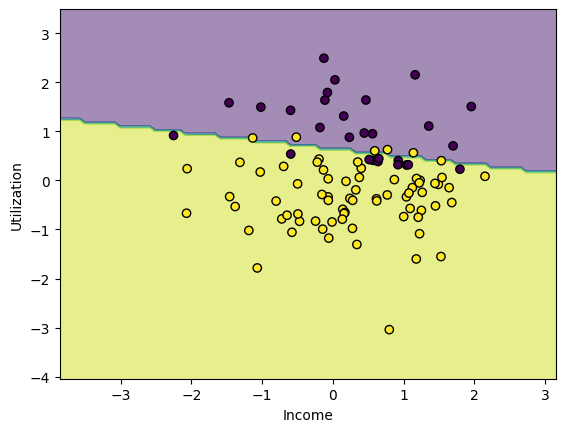
\includegraphics[width=\textwidth]{Figures/dbd_M.png}
                %   \caption{Decision boundary of $\mathcal{M}$}
                %   \label{fig:M_dbd}
                % \end{subfigure}%
                % \hfill
                % \begin{subfigure}[t]{.3\textwidth}
                %   \centering
                %   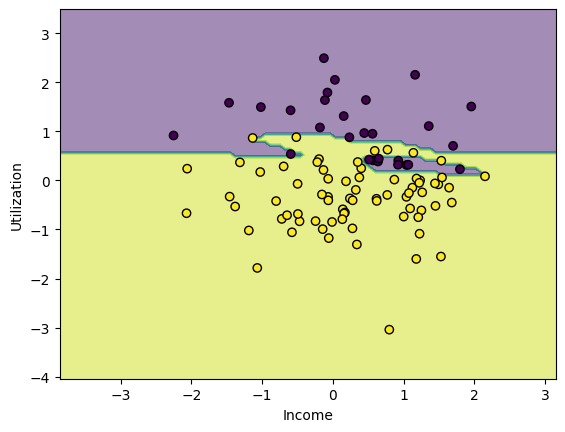
\includegraphics[width=\textwidth]{Figures/dbd_Mp.png}
                %   \caption{Decision Boundary of $\mathcal{M}_{\text{overfit}}$}
                %   \label{fig:Mp_dbd}
                % \end{subfigure}
                % \hfill
               \begin{subfigure}[t]{.28\textwidth}
                \centering
                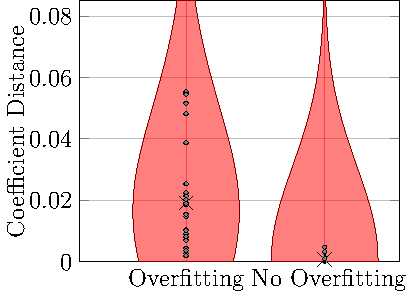
\includegraphics[width=\textwidth]{Figures/sec5_1_overfitting_spearmans.pdf}%{Figures/dbd_dists.png}
                %\caption{Effect of overfitting on stability}%Violin plots representing the stability of explainers of $\mathcal{M}$ and $\mathcal{M}_{\text{overfit}}$}
                \label{fig:dbd_dists}
                \end{subfigure}
                \caption{Violin plots representing the stability of explainers of $\mathcal{M}_1$ and $\mathcal{M}_2$. Each point represents the $L_2$ distance between the LIME coefficients for the explanation of a point near the decision boundary of $\mathcal{G}$ and its closest neighbor of the same class.}
                \label{fig:effect_of_overfitting}
            \end{figure}

            %\subsubsection{Decision Boundaries for Section on Decision Boundary Volatility}
            %    \label{sec:effect_of_overfitting}
                \begin{figure}[ht!]
                    \centering
                    \begin{subfigure}[t]{.28\textwidth}
                      \centering
                      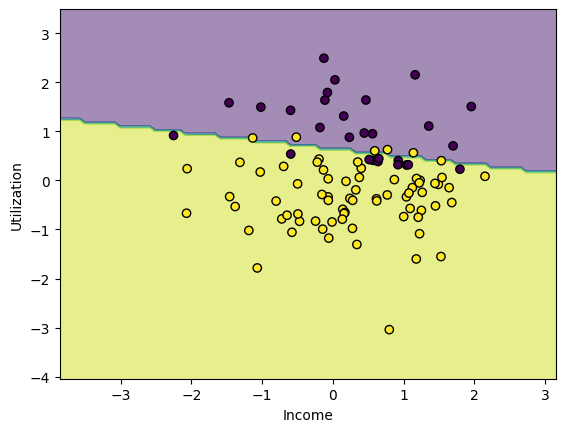
\includegraphics[width=\textwidth]{Figures/dbd_M.png}
                      \caption{Decision boundary of $\mathcal{M}$}
                      \label{fig:M_dbd}
                    \end{subfigure}%
                    \hspace{1cm}
                    \begin{subfigure}[t]{.28\textwidth}
                      \centering
                      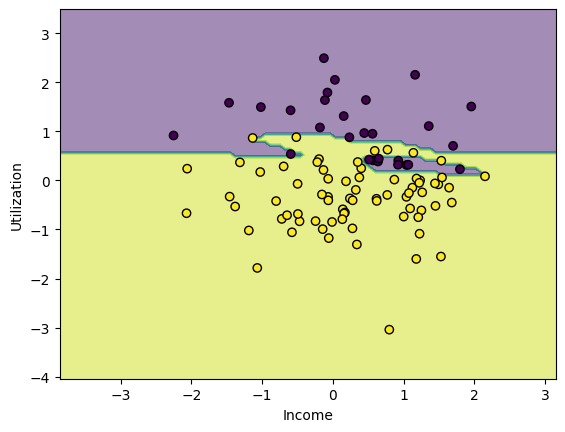
\includegraphics[width=\textwidth]{Figures/dbd_Mp.png}
                      \caption{Decision Boundary of $\mathcal{M}_{\text{overfit}}$}
                      \label{fig:Mp_dbd}
                    \end{subfigure}
                    \hspace{1cm}
                   \begin{subfigure}[t]{.28\textwidth}
                    \centering
                    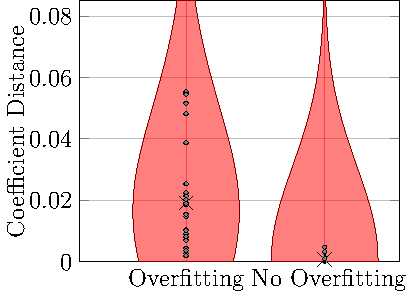
\includegraphics[width=\textwidth]{Figures/sec5_1_overfitting_spearmans.pdf}%{Figures/dbd_dists.png}
                    \caption{Effect of overfitting on stability}%Violin plots representing the stability of explainers of $\mathcal{M}$ and $\mathcal{M}_{\text{overfit}}$}
                    \label{fig:dbd_dists}
                    \end{subfigure}
                    \caption{Visualizations of decision boundaries for MLPs that do and do not overfit ($\mathcal{M}$ and $\mathcal{M}_{\text{overfit}}$) on a simple two variable loan approval dataset. Yellow points are accepted applicants and purple points are denied applicants.}
                    \label{fig:dbds}
                \end{figure}
        
        \subsubsection{Effect of Data Pre-processing}
        We identify two ways data pre-processing can affect post hoc explanations. First, the pre-processing affects the decision boundaries of models trained on it, which we know from Appendix Section \ref{sec:rashomon_overfitting} affects explanations. Second, pre-processing routines like standardization can change the signs of feature values, which we know from Section \ref{sec:theoretical_considerations} can cause the signs of a feature's Shapley value and marginal effect to differ.
            \begin{figure}[ht!]
                \centering
                %\begin{subfigure}{.28\textwidth}
                  \centering
                  \captionsetup{justification=centering}
                  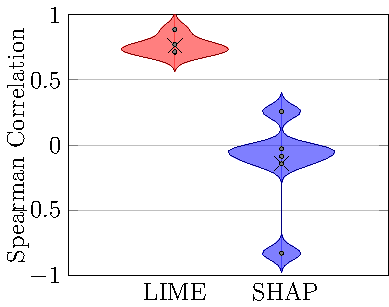
\includegraphics[width=.28\textwidth]{AppendixFigures/apx_preproc_rank_corrs.pdf}
                  %\caption{Correlations between feature rankings from explanation of model trained on standardized data with feature rankings from explanations of model trained on data with no pre-processing}%Spearman rank correlations of ranked feature importance magnitudes from LIME against the true ranked magnitudes from $\mathcal{G}$.}
                %   \label{fig:lime_income}
                %\end{subfigure}%
                \caption{Correlations between feature rankings from explanation of model trained on standardized data with feature rankings from explanations of model trained on data with no pre-processing}%Violin plots of feature importance values for \emph{income} from SHAP and LIME for cases when \emph{income} is unconfounded and confounded by the unobserved social support feature}
                \label{fig:lime_shap_preproc_corr}
            \end{figure}
    
    
    
   
    \subsection{Details on Mitigation Strategies}
        \label{apx_sec:mitigation_details}
        This section contains all the details for the hypothesis testing framework we use to evaluate our mitigation strategies. We motivate each test used and give the statements of the null and alternative hypotheses. 
        
        \subsubsection{Hypothesis Testing for Improvement}
            \label{sec:hypothesis_testing}
            In this section we will abuse notation and, for example, consider $\mE$ to be LIME with default settings explaining an MLP $\mathcal{M}_1$ and $\mE^\prime$ to be an explanation method that applies some mitigation strategies we propose. Thus, the notation $\mE$ and $\mE^\prime$ suppresses the models and data being used.
            
            Wilcoxon signed-rank tests are non-parametric tests for differences of populations, and thus applicable in our setting. Given two sets of measurements $A=\{a_i\}_{i=1}^m$ and $B=\{b_i\}_{i=1}^m$, Wilcoxon signed-rank tests operate on the matched differences $a_i-b_i$. We can view explanations from $\mE$ and $\mE^\prime$ as a matched sample since, for each $i$, $e_{\mE}(\mathbf{x}^{(i)})$ and $e_{\mE^\prime}(\mathbf{x}^{(i)})$ differ only by the explanation method used. We will assume that the differences are symmetrically distributed so that the null hypotheses declare the location of the population mean of the differences $a_i - b_i$. All tests will be performed with a significance level of $\alpha=.05$.
   
            \paragraph{Test for Equality of Directionality}        We have two conditions for $\mE^\prime$ to improve over $\mE$ with respect to directionality stating that 1) the sign accuracy of $\mE^\prime$ cannot be significantly worse than the sign accuracy of $\mE$ for any feature, and 2) the sign accuracy of $\mE^\prime$ must be significantly better than the sign accuracy of $\mE$ for at least one feature. We implement this using two Wilcoxon signed-rank tests for each feature. We consider, for each feature $j$, the null hypothesis
            \begin{equation*}
                H_0: \text{ The } s_j(e_\mE(x_j^{(i)},\beta_j) - s_j(e_{\mE^\prime}(x_j^{(i)},\beta_j) \text{ are symmetric about } \mu = 0
            \end{equation*}
            Then, to test if the directionality of $\mE^\prime$ was significantly worse than those of $\mE$, we test the following one-sided alternative hypotheses for each $j$.
            \begin{equation*}
                H_1: \text{ The } s_j(e_\mE(x_j^{(i)},\beta_j) - s_j(e_{\mE^\prime}(x_j^{(i)},\beta_j) \text{ are symmetric about } \mu > 0
            \end{equation*}
            If we reject $H_0$ in favor of $H_1$ at the $\alpha=.05$ level, we come to conclusion that $\mE^{\prime}$ did not improve over $\mE$ with respect to directionality. Otherwise, we move on to test the other one-sided alternative hypothesis for each $j$.
            \begin{equation*}
                H_2: \text{ The }  s_j(e_\mE(x_j^{(i)},\beta_j) - s_j(e_{\mE^\prime}(x_j^{(i)},\beta_j) \text{ are symmetric about } \mu < 0
            \end{equation*}
            If we reject $H_0$ in favor of $H_2$ for at least one $j$, we come to the conclusion that $\mE^{\prime}$ improved over $\mE$ with respect to directionality. Otherwise, we conclude that there was no significant change. 
            
            % are the ranks independent?
            % In pairs(x,y), x is a measurement for individual I and y is a measurement coming from an identical copy of I...
            \paragraph{Test for Equality of Concordance}  
            We say that $\mE^\prime$ improves over $\mE$ in terms of concordance based on the result of a Wilcoxon signed-rank test with the following null and alternative hypotheses.
            \begin{align*}
                H_0: \text{ The } \text{\text{concordance}}(e_\mE(\mathbf{x}^{(i)}),\boldsymbol{\beta}) - \text{\text{concordance}}(e_{\mE^\prime}(\mathbf{x}^{(i)})) \text{ are symmetric about } \mu=0 \\
                H_1: \text{ The } \text{\text{concordance}}(e_\mE(\mathbf{x}^{(i)}),\boldsymbol{\beta}) - \text{\text{concordance}}(e_{\mE^\prime}(\mathbf{x}^{(i)})) \text{ are symmetric about } \mu<0     \end{align*}
            That is, we must reject the null hypothesis that the concordance distributions of $\mE$ and $\mE^\prime$ have the same mean.        
            % cannot find implementation of multivariate KS test
            %Finally, we say that $E^\prime$ improve over $E$ in terms of relevance if a Kolmogorov-Smirnov (KS) test is significant at the $\alpha=.05$ level. The KS test is a non-parametric test for equality of (continuous) distributions. We use the multivariate extension  
            % is this not ok because the distributions for each k are related?
            \paragraph{Test for Equality of Relevance}         As with the directionality metric, have two conditions for $\mE^\prime$ to improve $\mE$ based on one sided Wilcoxon signed-rank tests. First, $\text{relevance}_k$ for $\mE^\prime$ cannot be significantly worse than the $\text{relevance}_k$ of $\mE$ for any $k$. Likewise, the $\text{relevance}_k$ of $E^\prime$ must be significantly better than the$\text{relevance}_k$ of $\mE$ for at least one $k$. We formulate the null and alternative hypotheses for each $k$ as follows.
            \begin{align*}
            H_0: \text{ The } \text{relevance}_k(r(e_\mE(\mathbf{x}^{(i)}), r(\boldsymbol{\beta})) - \text{relevance}_k(r(e_{\mE^\prime}(\mathbf{x}^{(i)}), r(\boldsymbol{\beta})) \text{ are symmetric about } \mu=0 \\
            H_1: \text{ The }\text{relevance}_k(r(e_\mE(\mathbf{x}^{(i)}), r(\boldsymbol{\beta})) - \text{relevance}_k(r(e_{\mE^\prime}(\mathbf{x}^{(i)}), r(\boldsymbol{\beta})) \text{ are symmetric about } \mu > 0 \\
            H_2: \text{ The } \text{relevance}_k(r(e_\mE(\mathbf{x}^{(i)}), r(\boldsymbol{\beta})) - \text{relevance}_k(r(e_{\mE^\prime}(\mathbf{x}^{(i)}), r(\boldsymbol{\beta})) \text{ are symmetric about } \mu<0      \end{align*}

            \paragraph{Tests for Equality of Consistency}
        We are interested in how consistent a method's feature importance values are across different factors of the pipeline when explaining a linear model since, ideally, they would always be data-aligned. Having established in Section \ref{sec:inconsistency} that different pairs of pipeline configurations often produce pairs of explanations such that the corresponding pairs of feature importance signs and rankings disagree, we will test for improvement of consistency in those two respects. To test whether a strategy improves consistency, we will compare a baseline pair of pipelines $\mE_1$ and $\mathcal{E}_2$ with a second pair of pipelines  $\mE^\prime_1$ and $\mE^\prime_2$ that employ the strategy we propose will improve consistency.

        We characterize improvement of consistency of feature importance signs by requiring that the feature importance signs from $\mE^\prime_1$ and $\mE^\prime_2$ are more consistent than those from $\mE_1$ and $\mE_2$ for at least one feature and not less consistent for any features. To test for this, for each of the $j=1,\ldots,d$ features, we utilize a one-sided McNemar test with the following contingency table, and null and alternative hypotheses involving matched samples of feature importance signs. Using the sign function ($\text{sgn}(0)=0$ and $\text{sgn}(x)=\frac{x}{\mid x\mid})$ otherwise), we define the following contingency table.
\begin{table}[h]
\centering
\begin{tabular}{|l|l|l|}
\hline
& $\text{sgn}(e_{\mE^\prime_1}(x_j^{(i)}))=\text{sgn}(e_{\mE^\prime_2}(x_j^{(i)}))$ & $\text{sgn}(e_{\mE^\prime_1}(x_j^{(i)}))\neq\text{sgn}(e_{\mE^\prime_2}(x_j^{(i)}))$ \\ \hline
$\text{sgn}(e_{\mE_1}(x_j^{(i)}))=\text{sgn}(e_{\mE_2}(x_j^{(i)}))$                  & a                                                                             & b                                                                                \\ \hline
$\text{sgn}(e_{\mE^\prime_1}(x_j^{(i)}))\neq\text{sgn}(e_{\mE^\prime_2}(x_j^{(i)}))$ & c                                                                             & d                                                                                \\ \hline
\end{tabular}
\caption{Contingency table used for McNemar's test of marginal equivalences applied to testing for improvement to the consistency of the feature importance sign given to feature $j$.}
\label{tab:my-table}
\end{table}
We define theoretical probabilities $p_a,p_b,p_c,p_d$ of occurrence in the cells $a,b,c,d$ such that $p_b$ and $p_c$ represent the probability that $\mE^\prime_1$ and $\mE^\prime_2$ give the same sign to a sample and the probability that $\mE_1$ and $\mE_2$ give the same sign to a sample, respectively. The null hypothesis asserts the equality of $p_b$ and $p_c$ and the alternative asserts that $p_b>p_c$, i.e. that the modified pipeline assigns feature importance signs more consistently.
        \begin{align*}
            & H_0: p_b = p_c \text{ (disagreement between $\mE_1$ and $\mE_2$ and disagreement between $\mE^\prime_1$ and $\mE^\prime_2$ is equally likely)}\\
            & H_1: p_b > p_c \text{ ($\mE_1$ and $\mE_2$ are more likely to disagree)} 
        \end{align*}
        Thus, improvement occurs if $H_0$ is rejected in favor of $H_1$ for at least one feature and $H_0$ is not rejected in favor of $H_2$ for any feature.

        
         We test for consistency of rankings as follows. Using the baseline pair of pipelines, we compute $C = \{\text{concordance}(e_{\mE_1}(\mathbf{x}^{(i)}), e_{\mE_2}(\mathbf{x}^{(i)}))\}_{i=1}^m$. Then, using the pair of pipelines involving the mitigation strategy of interest, we compute $C^\prime = \{\text{concordance}(e_{\mE^\prime_1}(\mathbf{x}^{(i)}), e_{\mE^\prime_2}(\mathbf{x}^{(i)}))\}_{i=1}^m$. We then perform a Wilcoxon signed-rank test with the following null and alternative hypotheses using $C$ and $C^\prime$ as matched samples. 
        \begin{align*}
            H_0: \text{ The } \text{concordance}(e_{\mE_1}(\mathbf{x}^{(i)}), e_{\mE_2}(\mathbf{x}^{(i)})) - \text{concordance}(e_{\mE^\prime_1}(\mathbf{x}^{(i)}), e_{\mE^\prime_2}(\mathbf{x}^{(i)})) \text{ are symmetric about } \mu=0 \\
            H_a: \text{ The } \text{concordance}(e_{\mE_1}(\mathbf{x}^{(i)}), e_{\mE_2}(\mathbf{x}^{(i)})) - \text{concordance}(e_{\mE^\prime_1}(\mathbf{x}^{(i)}), e_{\mE^\prime_2}(\mathbf{x}^{(i)})) \text{ are symmetric about } \mu > 0   
        \end{align*}
        
        % are disjoint sets of applicants so that $C$ and $C^\prime$ can be taken to be independent. 
        % Finally, we perform the following one-sided $F$-test for two variances at the $\alpha=.05$ significance level.

        % \begin{align*}
        %     H_0:\ \sigma_C^2 = \sigma_{C^\prime}^2 \\
        %     H_a:\ \sigma_C^2 < \sigma_{C^\prime}^2 \\
        % \end{align*}
        
        \subsubsection{SHAP Value Normalization}
            \label{sec:shap_norm_indep}

                Figure \ref{fig:dividex} shows a comparison of the results we obtained by comparing default SHAP explanations with SHAP explanations modified by normalizing by $(\mathbf{x}-\bar{\mathbf{x}})$. It shows that by normalizing the Shapley value, SHAP sees significant increases in directionality for all features, movement of the mean concordance from 0 to near 1, and noteworthy increases to $\text{relevance}_k$ for $k=2,\ldots,5$. Indeed, normalizing the Shapley value yields a significant improvement for each of our three metrics. This result suggests that normalizing the Shapley value is necessary to obtain data-aligned explanations using SHAP.
                    \begin{figure}[ht!]
                \centering
                \begin{subfigure}[t]{.28\textwidth}
                  \centering
                  \captionsetup{justification=centering}
                      \raisebox{.2cm}{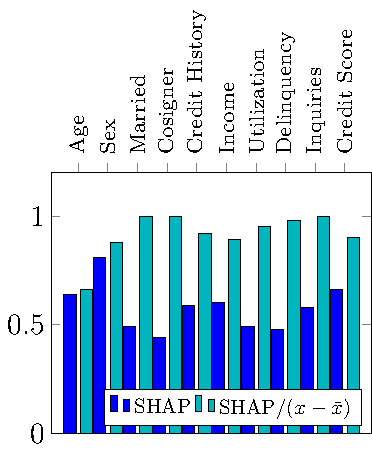
\includegraphics[width=\textwidth]{Figs/apx_dividex-figure0.pdf}}%{Figures/lime_shap_Spearman_magnitude.png}
    
                  \caption{SHAP Directionality}%Spearman rank correlations of feature importance magnitudes from SHAP and LIME against the true ranking from $\mathcal{G}$. }
                   \label{fig:dividex_sign_accs}
                \end{subfigure}%
                \hspace{1cm}
                \begin{subfigure}[t]{.28\textwidth}
                  \centering
                   \captionsetup{justification=centering}
                  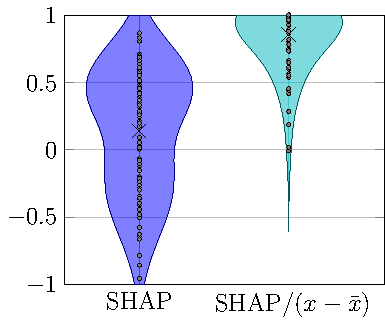
\includegraphics[width=\textwidth]{Figs/apx_dividex-figure1.pdf}%{Figures/lime_shap_Spearman_signed.png}
                  \caption{SHAP Concordance}%Spearman rank correlations of signed feature importance from SHAP and LIME against the true ranking from $\mathcal{G}$.}
                   \label{fig:dividex_spearmans}
                \end{subfigure}
                \hspace{1cm}
                \begin{subfigure}[t]{.28\textwidth}
                  \centering
                   \captionsetup{justification=centering}
                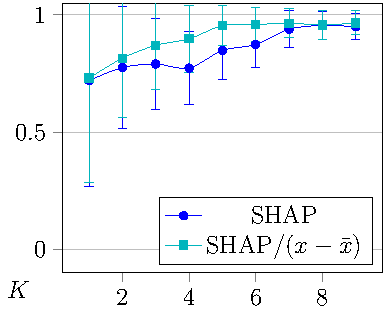
\includegraphics[width=\textwidth]{Figs/apx_dividex-figure2.pdf}%
                \caption{SHAP Relevance}%The average and standard error of recall of SHAP and LIME when attempting to capture the top K most important features to $\mathcal{G}$ when explaining $\mathcal{M}$, for varied $K=1,2,3,...$ number of features.}
                \label{fig:dividex_recalls}
                \end{subfigure}
                \caption{Comparison of default and normalized SHAP explanations with respect to directionality, concordance, and relevance.}
               \label{fig:dividex}
            \end{figure} 

    
    
    
    \subsection{Additional Mitigation Strategies}
        \label{apx_sec:additional_mitigations}
        In this section, we provide the results for mitigations strategies that we tried that are less effective or less intuitive/natural than those in the main paper. We first further explore different ways to use ensembles of explanations, then explore ways to select LIME explainers on the basis of their local predictive performance. 
        
        \subsubsection{Averaging Explanations Across Two Explainer Types}
            \label{sec:averaging_across_explainers}
            A simple way to resolve the difficulty in choosing whether to use SHAP or LIME is to use both and combine their results. In view of the fact that SHAP and LIME feature important values have different meanings, we propose to combine normalized Shapley values with LIME's feature importance values. 

            We did not find evidence that averaging SHAP and LIME together is beneficial. Figure \ref{fig:lime_shap_Spearman_together} shows that the averaged explanations were usually worse than those from LIME. We propose that this is because SHAP and LIME explanations generally do not satisfy criteria necessary for ensemble learning to be successful.   

            %use fbox to tailor crop
            \begin{figure}[ht!]
            \centering
                \begin{subfigure}{.28\textwidth}
                \centering
                %\fbox{\includegraphics[width=\textwidth,trim=0 10 70 70 mm, clip=true]{Figures/fig21.pdf}}%{Final_Figures/fig20.png}
                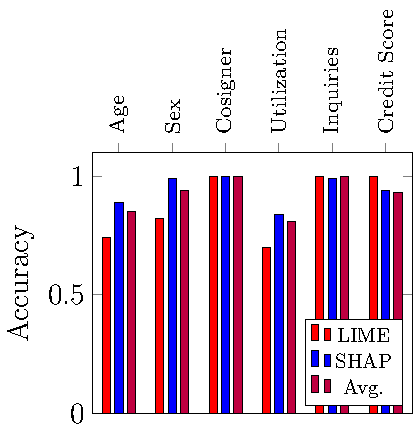
\includegraphics[width=\textwidth]{Figures/apx_limeshap-figure0.pdf}%{Figures/fig21.pdf}
                \caption{Directionality}
                \label{fig:lime_shap_Spearman_together}
                \end{subfigure}%
                \hspace{1cm}
                \begin{subfigure}{.28\textwidth}
                \centering
                %\fbox{\includegraphics[width=\textwidth,trim=0 10 70 70 mm, clip=true]{Figures/fig21.pdf}}%{Final_Figures/fig20.png}
                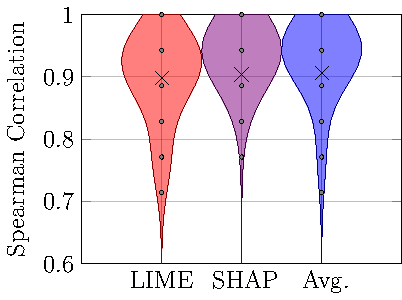
\includegraphics[width=\textwidth]{Figures/apx_limeshap-figure1.pdf}%{Figures/fig21.pdf}
                \caption{Relevance}
                \label{fig:lime_shap_Spearman_together}
                \end{subfigure}%
                \begin{subfigure}{.28\textwidth}
                \centering
                %\fbox{\includegraphics[width=\textwidth,trim=0 10 70 70 mm, clip=true]{Figures/fig22.p}%{Final_Figures/fig21.png}
                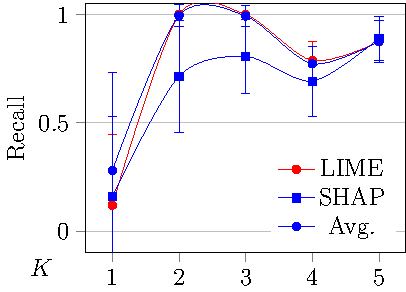
\includegraphics[width=\textwidth]{Figures/apx_limeshap-figure2.pdf}%{Figures/fig22.pdf}
                \caption{Relevance}
                \label{fig:lime_shap_Spearman_together_recall}
                \end{subfigure}
            \caption{Violin plots showing the effect of averaging SHAP and LIME explanations together on explanation quality and the ability to identify the most important features. }
            \label{fig:lime_shap_spearman_plots}
            \end{figure}


        \subsubsection{Voting Ensembles}
            Prior experiments handled ensembles of explanations by constructing the final ranking by ranking the features according to the average importance given to them over the component explanations. We hypothesize that this strategy could be improved by adding sophistication using voting strategies such as the borda count.  

            The Borda count is a ranked choice voting method. In it, every voter provides a ranking of the candidates. Each candidate is allocated a number of points from every ballot depending on what rank they were assigned. The point assignment method varies, but in the original formulation (which is used by the Slovenian Parliament), every candidate gets at least one point from each ballot. If there are $C$ candidates, the top ranked candidate gets in a ballot gets $C$ points, the runner up gets $C-1$ points, and so on until the lowest ranked candidate gets $1$ point. The candidate with the most points wins the election.

            The Borda count can be used to produce feature rankings for an input from LIME by making many LIME explainers by varying its hyperparameters and considering each LIME explainer to be a voter. We tested this method by comparing single explanations for each applicant with explanations formed from the Borda count results of 100 LIME explainers with random seeds $1,2,\ldots,100$.
            
            Our experiment did not provide evidence that the Borda count is an effective way to aggregate feature rankings. We show the results for spearman rank correlation and relevance metrics in Figure \ref{fig:borda_results} (since the Borda count operates on rankings, sign accuracy is not relevant). 

            \begin{figure}[ht!]
                \centering
                \begin{subfigure}[t]{.28\textwidth}
                  \centering
                   \captionsetup{justification=centering}
                  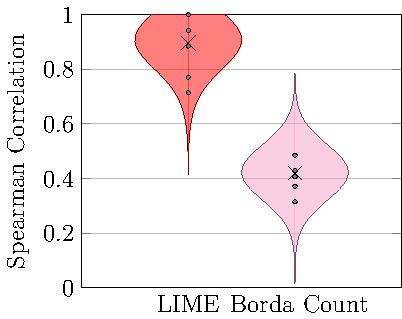
\includegraphics[width=\textwidth]{Figs/apx_borda-figure0.pdf}%{Figures/lime_shap_Spearman_signed.png}
                  \caption{Concordance}%Spearman rank correlations of signed feature importance from SHAP and LIME against the true ranking from $\mathcal{G}$.}
                   \label{fig:borda_spearmans}
                \end{subfigure}
                \hspace{1cm}
                \begin{subfigure}[t]{.28\textwidth}
                  \centering
                \captionsetup{justification=centering}
                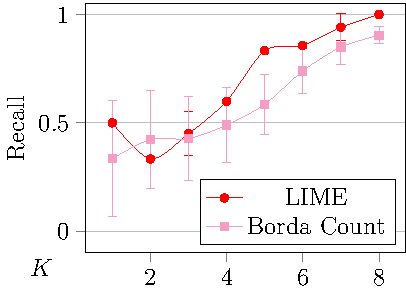
\includegraphics[width=\textwidth]{Figs/apx_borda-figure1.pdf}%
                \caption{Relevance}%The average and standard error of recall of SHAP and LIME when attempting to capture the top K most important features to $\mathcal{G}$ when explaining $\mathcal{M}$, for varied $K=1,2,3,...$ number of features.}
                \label{fig:borda_recalls}
                \end{subfigure}
                \caption{Comparisons of results for our three metrics for rankings from one LIME explainer compared with rankings obtained by applying the Borda count to rankings from 100 LIME explainers}
               \label{fig:borda_results}
            \end{figure} 

        \subsubsection{Averaging SHAP and LIME Explanations}
            Since SHAP and LIME have differing meanings of feature importance it does not make sense to aggregate them without further processing. We take two steps to address this. First, we normalize Shapley values (following Section \ref{sec:theoretical_considerations}) so that both SHAP and LIME can be seen as approximating $\boldsymbol{\beta}$. Then we max-normalized the SHAP and LIME values so that they occur on the same scale. 

            \begin{figure}[!h]
            \centering
                \begin{subfigure}[t]{0.28\textwidth}
                \centering
                \raisebox{.2cm}{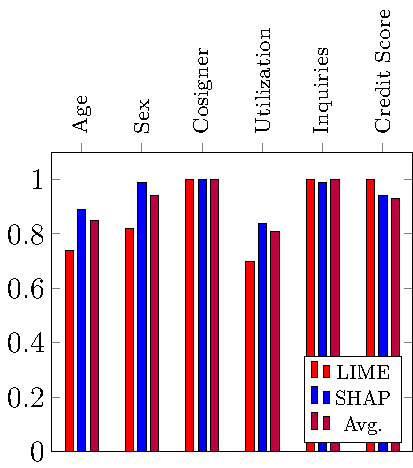
\includegraphics[width=\textwidth]{AppendixFigures/apx_limeshap-figure0.pdf}}
                \caption{Directionality} \label{fig:limeshap_sign_accs}
            \end{subfigure}\hspace{1cm}
            \begin{subfigure}[t]{0.28\textwidth}
                \centering
                \raisebox{.05cm}{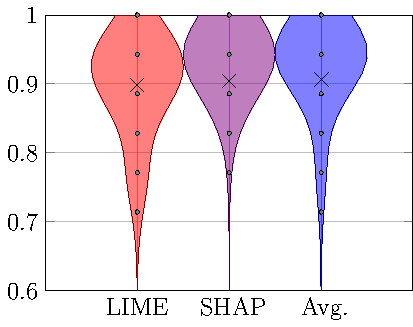
\includegraphics[width=\textwidth]{AppendixFigures/apx_limeshap-figure1.pdf}}
                \caption{Concordance} \label{fig:limeshap_spearmans}
            \end{subfigure}\hspace{1cm}
             \begin{subfigure}[t]{0.28\textwidth}
                \centering
                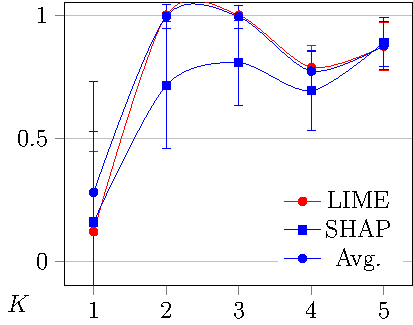
\includegraphics[width=\textwidth]{AppendixFigures/apx_limeshap-figure2.pdf}
                \caption{Relevance}
                \label{fig:limeshap_recalls}
            \end{subfigure}
            \caption{Comparison of individual LIME and (normalized) SHAP explanations with explanations constructed by averaging the feature importance values between the two for each applicant}\label{fig:limeshap}
            \end{figure}            

        \subsubsection{Ensuring that LIME's Local Prediction is Correct} 
            \label{sec:e_fidelity}
            Since the underlying linear model of a LIME explanation is constructed to be a good representative of $\mathcal{M}$'s local behavior, we hypothesized that the ability of a LIME explainer to correctly classify the label of the input being explained is related to the quality of the explanation for that input. Given an outcome $\mathcal{M}(\boldsymbol{\xi}) = y$ to be explained, the LIME package provides prediction probabilities for each possible label for $\boldsymbol{\xi}$. We will take $\hat{y}_{\text{LIME}}$ to be the label of the larger probability and attempt to clarify the relation between the condition $y = \hat{y}_{\text{LIME}}$ and the quality of LIME's explanations. In the Appendix, we also investigate how the local accuracy of LIME affects its explanation quality. 
        
            We only consider LIME here because LIME's surrogate model is a linear approximation of $\mathcal{M}$ and SHAP's is not; the idea of predictive accuracy makes sense for LIME and not SHAP. Indeed, the concept of local fidelity is only relevant for explainers using surrogate models. Counterfactual explanations, for example, do not have a notion of local fidelity. 
            
            %The local fidelity of an explainer's surrogate model is the surrogate model's prediction accuracy with respect to $\mathcal{M}$ in a neighborhood of the point being explained \citep{laugel18defining}. 
            %We will define fidIntuitively, high local fidelity should be associated with faithful explanations. This section investigates this claim. We use LIME alone in our experiments because LIME's surrogate model is a linear approximation of $\mathcal{M}$ and SHAP's is not; the idea of local fidelity in terms of function approximation only makes sense for LIME. The concept of local fidelity is only relevant for explainers using surrogate models. Counterfactual explainers, for example, have no notion of local fidelity. For our experiment, we create a set of LIME explainers of varying degrees of local fidelity and record the quality of their explanations. 
        
            For our experiment, we create a set of LIME explainers with different hyperparameters and, for 100 applicants, record whether they correctly classify the applicants' loan decision and the quality of their explanations for those applicants. We have LIME explain an MLP with AUC=.8 because if the AUC of $\mathcal{M}$ is very high, we observed that LIME surrogate models (almost) always correctly classify all loan decisions. For each applicant, we construct 100 LIME explainers using combinations of kernel widths $\nu$ in $\{.1\sqrt{d},.2\sqrt{d},\ldots,\sqrt{d}\}$ and random seeds $1,2,\ldots,10$. We do this because the kernel width and random seed determine the LIME surrogate model and therefore directly affect fidelity. We then evaluate our three faithfulness metrics for the resulting two families of LIME surrogate models. %We obtain the local fidelity of each $\mathcal{E}_{i,k}$ using LIME's built-in \emph{ score} function. 
                    
            %We also record the Spearman rank correlation of each feature ranking given by $\mathcal{E}_{i,k}$ and the ground truth. This allows us to associate local fidelity and explanation quality for each of the $\mathcal{E}_{i,k}$. We use the pairs of local fidelity and Spearman correlations to create a point plot in Figure \ref{fig:lime_fidelity}. 
        
            The results of our experiment suggest that ensuring that a LIME explainer's surrogate model correctly classifies the input being explained implies that the explainer may deserve additional confidence. We give violin plots of Spearman correlations of rankings for explanations given by LIME explainers whose underlying models correctly and incorrectly predicted the loan application decision in Figure \ref{fig:1pt_fid}. The figure shows that the mean concordanceis significantly larger for LIME explainers that correctly classify the input they are explaining. Additionally, the empirical concordancedistribution for correct LIMEs is more concentrated above .7 and has a much thinner left tail. Moreover, the LIME explainers that correctly classified loan approval decisions also generally had marginally better performance in finding the correct sign of feature importance values and identifying the top most important features. 
                    
            %Figure \ref{fig:lime_fidelity} reveals that as the fidelity of $\mathcal{E}$ increases, the quality of its explanations generally increases. The variance in explanation quality appears to decrease as local fidelity increases past 50\%. We hypothesize that the drop in concordancewhen the local fidelity is 100\% is due to overfitting. That is, the LIME surrogate model models the decision boundary of $\mathcal{M}$ too well and suffers as a result because $\mathcal{M}$ is an imperfect approximation of $\mathcal{G}$ and because local feature importance does not necessarily reflect the global feature importance in $\mathcal{G}$'s decision function.
        
                    % \begin{figure}[ht!]
                    %     \centering
                    %     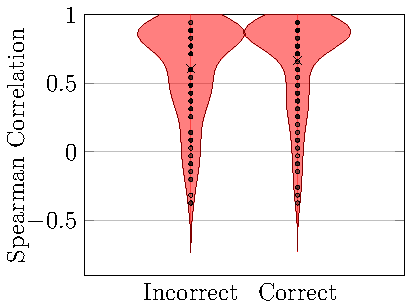
\includegraphics[width=.3\textwidth]{Figures/sec4_4_1pt_fid_spearmans.pdf}
                    %     \caption{Violin plots of Spearman correlations of feature rankings given by LIME explainers that did (right) and did not (left) correctly classify the input they were explaining}%Point plot for LIME's local fidelity versus its explanation quality, measured via Spearman rank correlation. Points indicate means and the vertical bars at each fidelity level indicate the 95\% confidence interval for the concordancetaken over all the models that had that level of accuracy.}
                    %     \label{fig:lime_fidelity}
                    % \end{figure}
                    
            \begin{figure}[ht!]
                \centering
                \begin{subfigure}[t]{.28\textwidth}
                  \centering
                  \captionsetup{justification=centering}
                      \raisebox{.2cm}{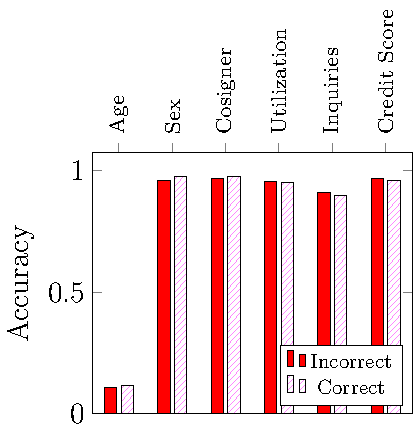
\includegraphics[width=\textwidth]{Figs/sec4_4_1pt_fid-figure0.pdf}}%{Figures/lime_shap_Spearman_magnitude.png}
    
                  \caption{Directionality}%Spearman rank correlations of feature importance magnitudes from SHAP and LIME against the true ranking from $\mathcal{G}$. }
                   \label{fig:1pt_sign_accs}
                \end{subfigure}%
                \hspace{1cm}
                \begin{subfigure}[t]{.28\textwidth}
                  \centering
                   \captionsetup{justification=centering}
                  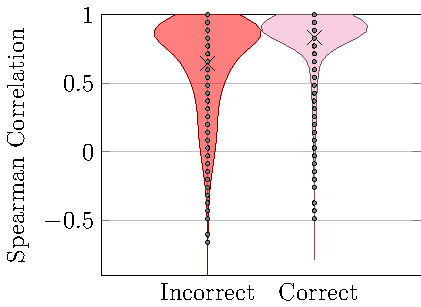
\includegraphics[width=\textwidth]{Figs/sec4_4_1pt_fid-figure1.pdf}%{Figures/lime_shap_Spearman_signed.png}
                  \caption{Concordance}%Spearman rank correlations of signed feature importance from SHAP and LIME against the true ranking from $\mathcal{G}$.}
                   \label{fig:1pt_spearmans}
                \end{subfigure}
                \hspace{1cm}
                \begin{subfigure}[t]{.28\textwidth}
                  \centering
                \captionsetup{justification=centering}
                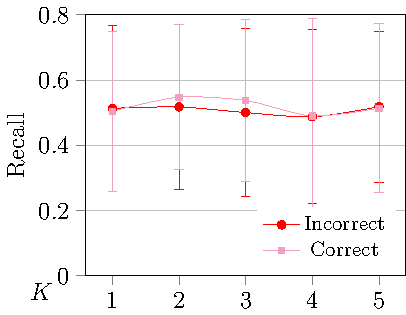
\includegraphics[width=\textwidth]{Figs/sec4_4_1pt_fid-figure2.pdf}%
                \caption{Relevance}%The average and standard error of recall of SHAP and LIME when attempting to capture the top K most important features to $\mathcal{G}$ when explaining $\mathcal{M}$, for varied $K=1,2,3,...$ number of features.}
                \label{fig:1pt_recalls}
                \end{subfigure}
                \caption{Comparisons of results for our three metrics for LIME explainers whose surrogate models do and do not correctly classify the loan decision of applicants they are explaining.}
               \label{fig:1pt_fid}
            \end{figure} 
        
        
            % Intuition dictates that as the local fidelity of the surrogate model of an explainer $\mathcal{E}$ increases, the quality of the explanations from $\mathcal{E}$ should also increase. Assuming that $\mathcal{M}$ is a good representation of $\mathcal{G}$, this sets $\mathcal{E}$ up to also represent $\mathcal{G}$ well. Although there generally seems to be a positive correlation between local fidelity and average explanation quality, the wild variance of explanation quality, especially for lower local fidelities, makes this relationship less clear. We hypothesize that the lack of clarity here is related to the fact that LIME regressors are fit on sampled data, some of which may be out of distribution \citep{rahnama19shift}.
            
            %It is not clear, however, what the impact of the fidelity of $\mathcal{E}$ is on explanation quality aside from very low and very high fidelities making explanation quality vary wildly. We hypothesize that the lack of clarity here is related to the fact that LIME regressors are fit on sampled data, some of which may be out of distribution \citep{rahnama19shift}.
        
    
        
            
   
    
    %\subsection{Mitigation Strategies for Inconsistency} 
    %    \label{sec:inconsistency_mitigation}
 
    

        \subsubsection{Increasing LIME's Local Fidelity}
            In Section \ref{sec:} we established an association between the quality of a LIME explainer $\mathcal{E}$'s explanation of $y=\mathcal{M}(\boldsymbol{\xi})$ and whether $\mathcal{E}(\boldsymbol{\xi}) = y$. We will explore here whether the accuracy of $\mathcal{E}$ on data in $\text{B}_\nu(\boldsymbol{\xi})$, the neighborhood of data samples within $\nu$ of $\boldsymbol{\xi}$. 

        %\subsubsection{Weak Learner LIMEs}

        % \subsubsection{Pearl's Backdoor Adjustment}
        %     \label{sec:backdoor_adjustment}

    %n -> i
    % add closed form for SHAP
    
    

    
    
    \subsection{Details on Econometric Case Study}
        \label{apx_sec:econometric_details}
        It was necessary to use simulated data for most of our experiments because we needed control over the ground truth and data generation process, but we needed a real dataset and accompanying econometric results to gauge how well SHAP and LIME could reproduce those results. This case study is motivated in part by the pattern we noticed in our case study where authors express an affinity for explaining ML models instead of using econometrics methods. 
        
        The data for the case study is a well known dataset used in textbooks such as \cite{}. It originally appeared in \cite{}, but we use the regression results of \cite{} as the ground truth for the case study. The meanings of the feature names were obtained \citep{HunterWilliamC1996Tcah} and are provided below in Table \ref{tab:case_study_features}.
        
        \begin{table}[ht!]
            \centering
            \begin{tabular}{|l|l|l|}
            \hline
            \textbf{Feature} & \textbf{Meaning}                   & \textbf{Range}                \\ \hline
            %gdlin            & credit history meets guidelines    & binary                        \\ \hline
            good credit            & credit history meets guidelines    & binary                        \\ \hline
            %typur            & type of purchaser of loan          & 0,1,2,\textbackslash{}ldots,9 \\ \hline
            purchaser type            & type of purchaser of loan          & 0,1,2,\textbackslash{}ldots,9 \\ \hline
            %inson            & \makecell{approved for private mortage insurance (PMI)}                      & binary                        \\ \hline
            PMI approved            & \makecell{approved for private mortage insurance (PMI)}                      & binary                        \\ \hline
            %prop             & type of property                   & binary                        \\ \hline
            multi family     & \makecell{purchasing 2-4 family home \\ versus 1 family home or condo } \\ \hline
            unver            & unverifiable info                  & binary                        \\ \hline
            %fixadj           & fixed or adjustable rate           & binary                        \\ \hline
            fixed rate           & fixed or adjustable rate           & binary                        \\ \hline
            %pubrec           & filed bankruptcy                   & binary                        \\ \hline
            bankruptcy           & filed bankruptcy                   & binary                        \\ \hline
            %vr               & tract vac rte \textgreater msa med & binary                        \\ \hline
            value rate               & \makecell{whether the rental income in tract \\ divided by estimate of value \\\ of rental property \textgreater Boston median} & binary                        \\ \hline
            %obrat            & \makecell{percentages of housing expenditures \\ and other obligations \\ normalized by total income}    & {[}0,100{]}                   \\ \hline
            debt rate           & \makecell{percentages of housing expenditures \\ and other obligations \\ normalized by total income}    & {[}0,100{]}                   \\ \hline
            old              & applicant age \textgreater Boston median & binary                        \\ \hline
            married          & if applicant married               & binary                        \\ \hline
            gift             & gift as down payment               & binary                         \\
            \hline
            \end{tabular}
            \caption{Feature meanings and ranges for the case study}
            \label{tab:case_study_features}
        \end{table}

%\subsection{Guidance For Use of post hoc Explainers}
%    \subsubsection{Compare Explanations With Those From Decision Trees}

  

    
    
    \subsection{Repetition of Main Experiments on Marketing Dataset}
        \label{apx_sec:marketing}
        To further support our findings, we present here the results of all experiments in the main body of the paper (less the econometric case study) using a synthetic direct marketing example. The meanings of the features and how they were generated is summarized in Table \ref{tab:marketing_simulated}. Unlike the loan application dataset, the direct marketing dataset contains categorical features. We binarize the categorical features, which contributes to this dataset having more features than the loan application dataset (15 versus 10). We will see in the next section that there is a tendency for dataset with more features to have less data-aligned explanations.


\begin{table}[h]
\centering
\resizebox{\textwidth}{!}{%
\begin{tabular}{c|c|c}
\toprule
\textsc{Feature} & \textsc{Explanation}                           & \textsc{Formula}       \\ \toprule
Age              & Customer Age                                   & Uniform(18,100)        \\ 
Sex              & Customer Sex                                   & Bernoulli(.5)          \\
Married          & Customer Marital Status                        & Bernoulli(.5)          \\ 
Education           & Customer Education Level                                & High School, College, or Graduate \\ 
Previous Purchase        & Whether product previously purchased                      & Bernoulli(.5)          \\ 
Website Visits         & Number of Times Website Visited & Uniform(0,50)         \\ 
Subscribed      & Subscribed to Regular Ads            & Bernoulli(.5)           \\ 
Offer Type     & Type of offer in Ad  & Discount, BOGO, or Free Shipping \\
Offer Value    & Value of offer in Ad & Depends on Subscription status          \\ 
Mode     & Way advertisement is delivered & Email, SMS, or Social Media \\           \\ \bottomrule
\end{tabular}%
}
\caption{Description of features for simulated direct marketing data.}
\label{tab:marketing_simulated}
\end{table}
        \subsubsection{Baseline}
            Figure \ref{fig:marketing_beta_alignment} shows a comparison between SHAP and LIME with their default settings and a random explainer when explaining a model with test set ROC AUC of XX that was trained on the marketing dataset described in Table \ref{tab:marketing_simulated}. We reach the same conclusion as in Section \ref{sec:misalignment}, that is that LIME does fairly well with respect to all three metrics while SHAP is not significantly better than a random explainer except with respect to relevance.
            
            \begin{figure}[ht!]
                \centering
                \begin{subfigure}[t]{.28\textwidth}
                  \centering
                  \captionsetup{justification=centering}
                      \raisebox{.2cm}{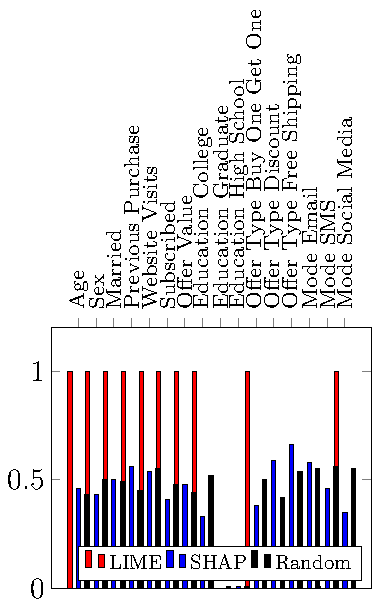
\includegraphics[width=\textwidth]{MarketingFigs/sec4_1-figure0.pdf}}%{Figures/lime_shap_Spearman_magnitude.png}
    
                  \caption{Directionality}%Spearman rank correlations of feature importance magnitudes from SHAP and LIME against the true ranking from $\mathcal{G}$. }
                   \label{fig:lime_shap_sign_accs}
                \end{subfigure}%
                \hspace{1cm}%\hfill
                \begin{subfigure}[t]{.28\textwidth}
                  \centering
                   \captionsetup{justification=centering}
                  \raisebox{.05cm}{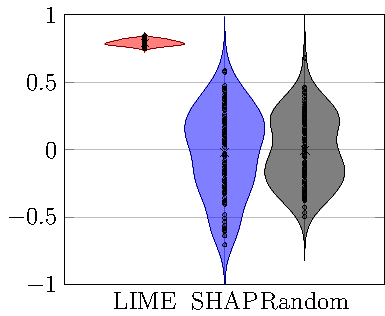
\includegraphics[width=\textwidth]{MarketingFigs/sec4_1-figure1.pdf}}%{Figures/lime_shap_Spearman_signed.png}
                  \caption{Concordance}%Spearman rank correlations of signed feature importance from SHAP and LIME against the true ranking from $\mathcal{G}$.}
                   \label{fig:lime_shap_Spearman_signed}
                \end{subfigure}
                \hspace{1cm}%\hfill
                \begin{subfigure}[t]{.28\textwidth}
                  \centering
                   \captionsetup{justification=centering}
                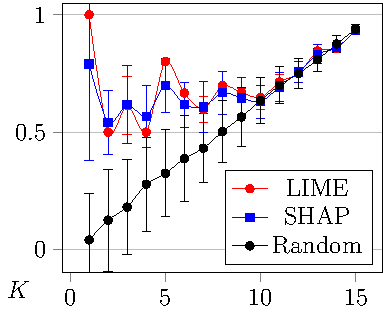
\includegraphics[width=\textwidth]{MarketingFigs/sec4_1-figure2.pdf}%
                \caption{Relevance}%The average and standard error of recall of SHAP and LIME when attempting to capture the top K most important features to $\mathcal{G}$ when explaining $\mathcal{M}$, for varied $K=1,2,3,...$ number of features.}
                \label{fig:avg_recall}
                \end{subfigure}
                \caption{Bar plot of directionality, violin plot of concordance, and line plot for relevance$_k$. For plot (c) Each point in the line plot represents a mean relevance for a given $k$. The error bars represent the standard error. The total number of features is 16.}
               \label{fig:marketing_beta_alignment}
            \end{figure}   

        \subsubsection{SHAP Normalization}
            As in Section \ref{sec:theoretical_considerations}, we check whether SHAP normalization is useful when working with the direct marketing dataset. Figure \ref{fig:marketing_shap_dividex_corr} shows that this is indeed the case if not only because concordance increased greatly. Additionally, directionality for many features increased from nearly .5 to nearly 1. 


           \begin{figure}[ht!]
            \centering
            \begin{subfigure}[t]{.28\textwidth}
              \centering
              \captionsetup{justification=centering}
                  \raisebox{.2cm}{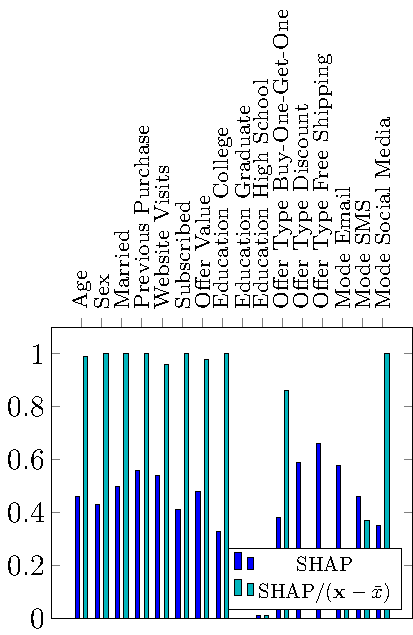
\includegraphics[width=\textwidth]{MarketingFigs/shap_dividex-figure0.pdf}}%{Figures/lime_shap_Spearman_magnitude.png}

              \caption{Directionality}%Spearman rank correlations of feature importance magnitudes from SHAP and LIME against the true ranking from $\mathcal{G}$. }
               \label{fig:marketing_shap_dividex_accs}
            \end{subfigure}%
            \hspace{1cm}%\hfill
            \begin{subfigure}[t]{.28\textwidth}
              \centering
               \captionsetup{justification=centering}
              \raisebox{.05cm}{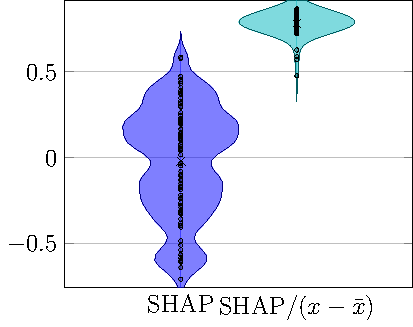
\includegraphics[width=\textwidth]{MarketingFigs/shap_dividex-figure1.pdf}}%{Figures/lime_shap_Spearman_signed.png}
              \caption{Concordance}%Spearman rank correlations of signed feature importance from SHAP and LIME against the true ranking from $\mathcal{G}$.}
               \label{fig:marketing_shap_dividex_spearmans}
            \end{subfigure}
            \hspace{1cm}%\hfill
            \begin{subfigure}[t]{.28\textwidth}
              \centering
               \captionsetup{justification=centering}
            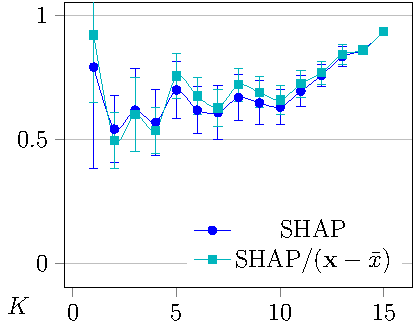
\includegraphics[width=\textwidth]{MarketingFigs/shap_dividex-figure2.pdf}%
            \caption{Relevance}%The average and standard error of recall of SHAP and LIME when attempting to capture the top K most important features to $\mathcal{G}$ when explaining $\mathcal{M}$, for varied $K=1,2,3,...$ number of features.}
            \label{fig:marketing_shap_dividex_recalls}
            \end{subfigure}
            \caption{Comparison of SHAP explanations without and with SHAP value normalization}
           \label{fig:marketing_shap_dividex_corr}
        \end{figure}   

        \subsubsection{Role of Predictive Performance of $\mathcal{M}$ - \textcolor{red}{Double check!!!}}
            To test the effect of the predictive performance of $\mathcal{M}$, we compare explanations of models $\mathcal{M}_1$ with AUC XX, $\mathcal{M}_2$ with AUC YY, and $\mathcal{M}_3$ with AUC ZZ. The results of our comparison, illustrated below in Figure \ref{fig:}, show that although directionality was not significantly impacted for SHAP or LIME, increasing the model AUC did have substantial effects on concordance and relevance. SHAP's concordance.
        \begin{figure}[t!]
            \subfloat[SHAP Directionality]{%
                \raisebox{.2cm}{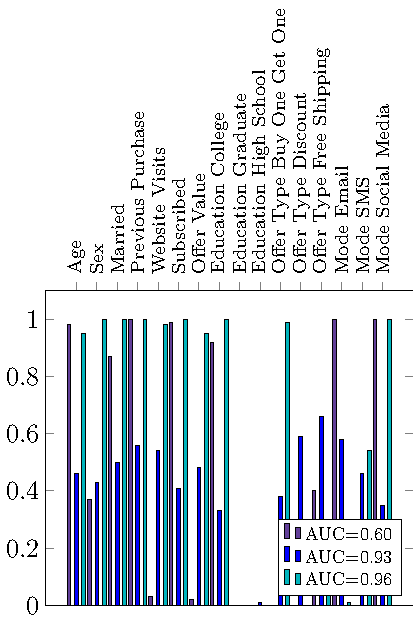
\includegraphics[width=.28\textwidth]{MarketingFigs/sec4_4_mlp_auc_shap-figure0.pdf}}%
                \label{subfig:marketing_mlp_avg_shap_sign_accs}%
            }\hspace{1cm}
            \subfloat[SHAP Concordance]{%
                 \raisebox{.05cm}{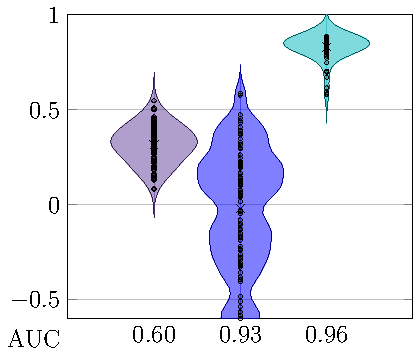
\includegraphics[width=.28\textwidth]{MarketingFigs/sec4_4_mlp_auc_shap-figure1.pdf}}%
                \label{subfig:marketing_mlp_auc_shap_spearmans}%
            }\hspace{1cm}
            \subfloat[SHAP Relevance]{%
                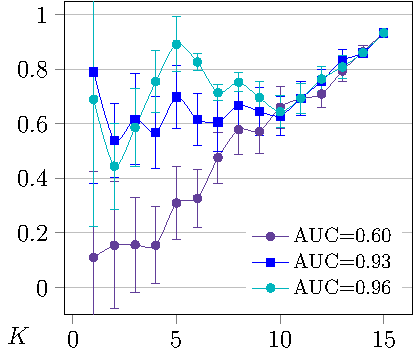
\includegraphics[width=.28\textwidth]{MarketingFigs/sec4_4_mlp_auc_shap-figure2.pdf}%
                \label{subfig:marketing_mlp_auc_shap_recalls}%
            }\\
            \subfloat[LIME Directionality]{%
                \raisebox{.2cm}{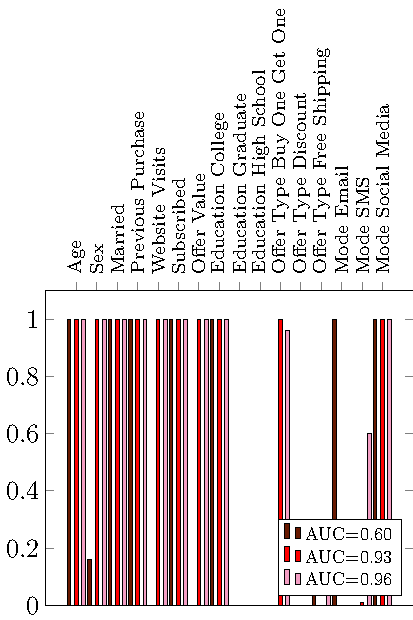
\includegraphics[width=.28\textwidth]{MarketingFigs/sec4_4_mlp_auc_lime-figure0.pdf}}%
                \label{subfig:marketing_mlp_auc_lime_sign_accs}%
            }\hspace{1cm}%\hfill
            \subfloat[LIME Concordance]{%
                \raisebox{.05cm}{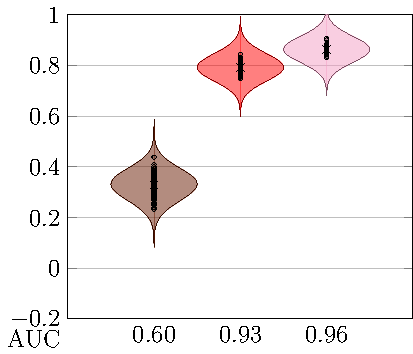
\includegraphics[width=.28\textwidth]{MarketingFigs/sec4_4_mlp_auc_lime-figure1.pdf}}%
                \label{subfig:marketing_mlp_auc_lime_spearmans}%
            }\hspace{1cm}
            \subfloat[LIME Relevance]{%
                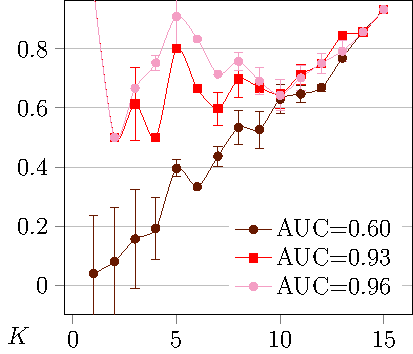
\includegraphics[width=.28\textwidth]{MarketingFigs/sec4_4_mlp_auc_lime-figure2.pdf}%
                \label{subfig:marketing_mlp_auc_lime_recalls}%
            }\\
            \caption{Comparisons of results for our three metrics for SHAP and LIME when explaining $\mathcal{M}_1$ with AUC=.6, $\mathcal{M}_2$ with AUC=0.92, and $\mathcal{M}_3$ with AUC=.99}
            \label{fig:marketing_mlp_auc_increase}
        \end{figure}


        \subsubsection{Role of Feature Independence}
            Following Section \ref{sec:}, we alter the direct marketing dataset to make the features independent but do not change the formula for $\mathcal{G}(\mathbf{X})$. The only change made is to change``Offer Value" from being a function of subscription status to becoming distributed according to XYZ.

            It was again the case that explanations of the model trained on data with independent features were more data aligned. In particular, Figure \ref{fig:} shows that explanations of the model trained on the version of the marketing dataset with independent features had a mean concordance which was about .1 larger and relevances for $k=2,3,4$ which were up to .5 larger. 
            
            \begin{figure}[t!]
                \subfloat[SHAP Directionality]{%
                    \raisebox{.2cm}{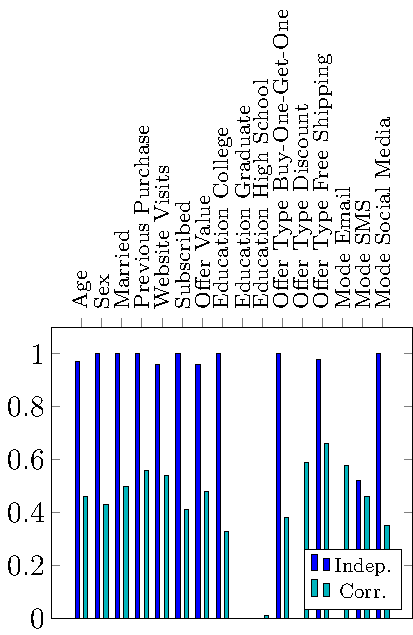
\includegraphics[width=.28\textwidth]{MarketingFigs/shap_corr-figure0.pdf}}%
                    \label{fig:marketing_shap_corr_accs}%
                }\hspace{1cm}%\hfill
                \subfloat[SHAP Concordance]{%
                    \raisebox{.05cm}{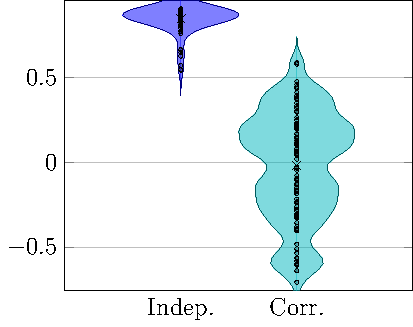
\includegraphics[width=.28\textwidth]{MarketingFigs/shap_corr-figure1.pdf}}%
                    \label{fig:marketing_shap_corr_spearmans}%
                }\hspace{1cm}%\hfill
                \subfloat[SHAP Relevance]{%
                    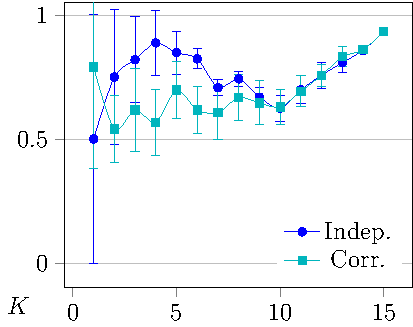
\includegraphics[width=.28\textwidth]{MarketingFigs/shap_corr-figure2.pdf}%
                    \label{fig:marketing_shap_corr_recalls}%
                }\\
                \subfloat[LIME Directionality]{%
                    \raisebox{.2cm}{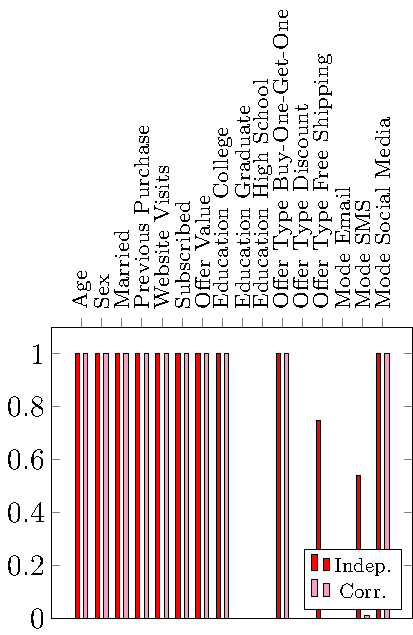
\includegraphics[width=.28\textwidth]{MarketingFigs/lime_corr-figure0.pdf}}%
                    \label{fig:marketing_lime_corr_accs}%
                }\hspace{1cm}%\hfill
                \subfloat[LIME Concordance]{%
                    \raisebox{.05cm}{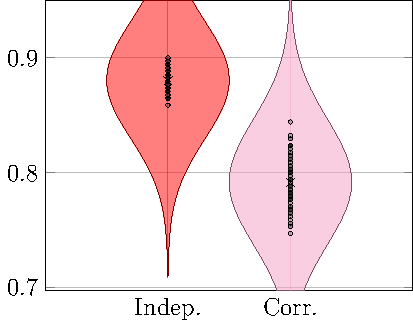
\includegraphics[width=.28\textwidth]{MarketingFigs/lime_corr-figure1.pdf}}%
                    \label{fig:marketing_lime_corr_spearmans}%
                }\hspace{1cm}%\hfill
                \subfloat[LIME Relevance]{%
                    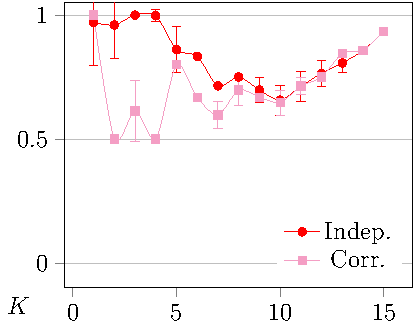
\includegraphics[width=.28\textwidth]{MarketingFigs/lime_corr-figure2.pdf}%
                    \label{fig:marketing_lime_corr_recalls}%
                }\\
                \caption{Comparison of faithfulness of explanations of models trained on data with independent features versus data with two strongly correlated features.}
                \label{fig:marketing_lime_shap_colinear}
            \end{figure}

        \subsubsection{Increasing $\nu$ and $n$ for LIME}
            The effect of increasing $\nu$ and $n$ may not be immediately apparent from Figure \ref{fig:marketing_lime_tuning}, but it does show directionality was increased for some features and not lower for any other feature except ``website visits". Directionality for ``Offer Type: Free Shipping" was significantly increased with $p<.001$ while directionality for ``Mode: SMS" was increased insignificantly with $p\simeq.07$. Concordance was slightly lower when $\nu=n=10000$. Relevance was significantly better for $k=1,3$ with $p\simeq.004$.
            \begin{figure}[ht!]
                \centering
                \begin{subfigure}[t]{.28\textwidth}
                  \centering
                  \captionsetup{justification=centering}
                      \raisebox{.2cm}{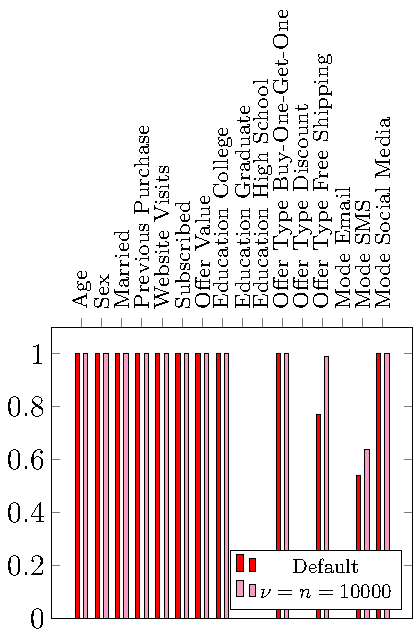
\includegraphics[width=\textwidth]{MarketingFigs/lime_nu_N-figure0.pdf}}%{Figures/lime_shap_Spearman_magnitude.png}
    
                  \caption{Directionality}%Spearman rank correlations of feature importance magnitudes from SHAP and LIME against the true ranking from $\mathcal{G}$. }
                   \label{fig:marketing_lime_tuning_sign_accs}
                \end{subfigure}%
                \hspace{1cm}
                \begin{subfigure}[t]{.28\textwidth}
                  \centering
                   \captionsetup{justification=centering}
                  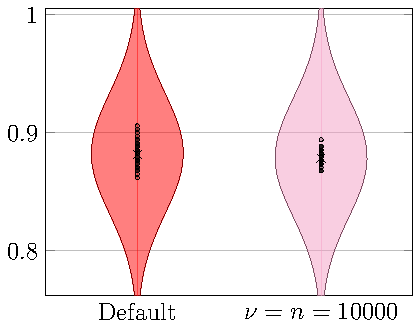
\includegraphics[width=\textwidth]{MarketingFigs/lime_nu_N-figure1.pdf}%{Figures/lime_shap_Spearman_signed.png}
                  \caption{Concordance}%Spearman rank correlations of signed feature importance from SHAP and LIME against the true ranking from $\mathcal{G}$.}
                   \label{fig:marketing_lime_tuning_spearmans}
                \end{subfigure}
                \hspace{1cm}
                \begin{subfigure}[t]{.28\textwidth}
                  \centering
                   \captionsetup{justification=centering}
                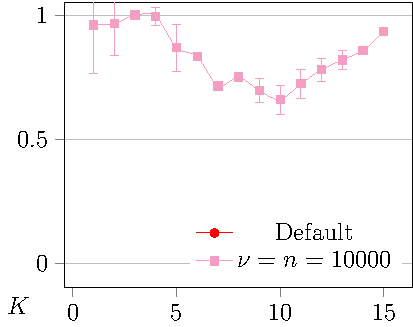
\includegraphics[width=\textwidth]{MarketingFigs/lime_nu_N-figure2.pdf}%
                \caption{Relevance}%The average and standard error of recall of SHAP and LIME when attempting to capture the top K most important features to $\mathcal{G}$ when explaining $\mathcal{M}$, for varied $K=1,2,3,...$ number of features.}
                \label{fig:marketing_lime_tuning_recalls}
                \end{subfigure}
                \caption{Comparison of LIME explainer with default settings versus $\nu=n=10000$ with respect to our three metrics}
               \label{fig:marketing_lime_tuning}
            \end{figure} 

        \subsubsection{Averaging Explanations of One Model by Different Explainers}
            We again tested whether averaging the explanations of one model by 10 LIME explainers with different random seeds was useful. The results of the experiment are given in Figure \ref{fig:} and show that directionality increased appreciably for a few features while it was unchanged for the others, there was not a significant change to concordance, and there was some improvement to relevance for small $k$. 

            As for directionality, ``Mode: SMS" was increased with $p\simeq .01$, ``Offer Type: Free Shipping" increased with $p<.001$, and the other features were unaffected except for ``Website Visits" which was worse with $p<.001$. Concordance was very slightly lower. Relevance was significantly increased for $k=1$  with $p\simeq .004$, insignificantly increased for $k=3$ with $p\simeq .07$. 

            The strategy increased the consistency in some respects. Feature importance signs were more consistent with $p\simeq .1$ for ``Mode: SMS" and significantly more consistent for ``Offer Type: Free Shipping" with $p<.001$. The rankings were significantly more consistent with $p<.001$. 
            \begin{figure}[!h]
            \centering
                \begin{subfigure}[t]{0.28\textwidth}
                \centering
                \raisebox{.2cm}{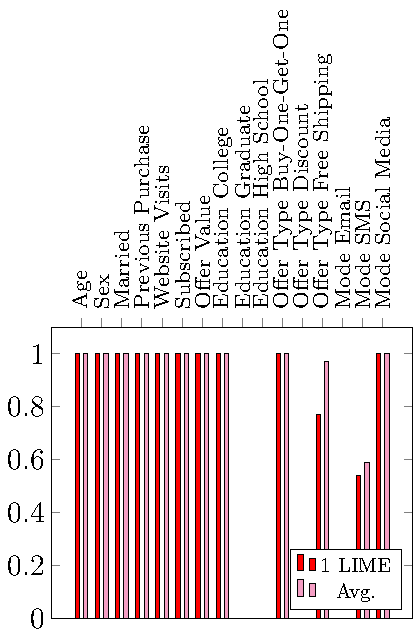
\includegraphics[width=\textwidth]{MarketingFigs/lime_avg-figure0.pdf}}
                \caption{Directionality} \label{fig:marketing_lime_avg_sign_accs}
            \end{subfigure}\hspace{1cm}
            \begin{subfigure}[t]{0.28\textwidth}
                \centering
                \raisebox{.05cm}{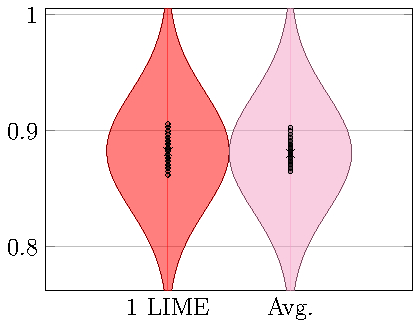
\includegraphics[width=\textwidth]{MarketingFigs/lime_avg-figure1.pdf}}
                \caption{Concordance} \label{fig:marketing_lime_avg_spearmans}
            \end{subfigure}\hspace{1cm}
             \begin{subfigure}[t]{0.28\textwidth}
                \centering
                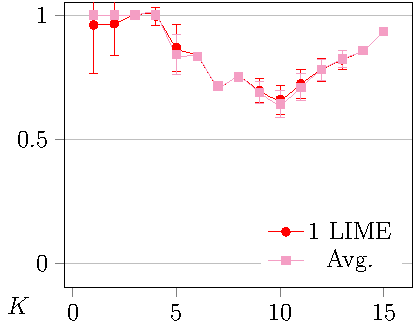
\includegraphics[width=\textwidth]{MarketingFigs/lime_avg-figure2.pdf}
                \caption{Relevance}
                \label{fig:marketing_lime_avg_recalls}
            \end{subfigure}
            \caption{Comparisons of results for our three metrics for  explanations of an MLP $\mathcal{M}$ by 1 LIME explainer versus those created by averaging the feature importance values of 100 LIME explanations of $\mathcal{M}$}\label{fig:marketing_lime_avg}
            \end{figure}

        \subsubsection{Averaging Explanations of Different Models}
            The models we used for averaging all had test set AUCs of .96 and test set accuracies of .89. It is easily seen from the visualization of the experimental results in Figure \ref{fig:} that this strategy was beneficial because the concordances are noticeably larger for both SHAP and LIME. 

            With regard to directionality for SHAP, ``Offer Type: Free Shipping" and ``Website visits" were the two features that significantly increased, as they had $p<.001$. Concordance significantly increased with $p<.001$. Relevance was significantly increased for $k=1,12$. It also increased for the other $k$, but not significantly at the $\alpha=.05$ level. 
            
            \begin{figure}[t!]
                \subfloat[SHAP Directionality]{%
                    \raisebox{.2cm}{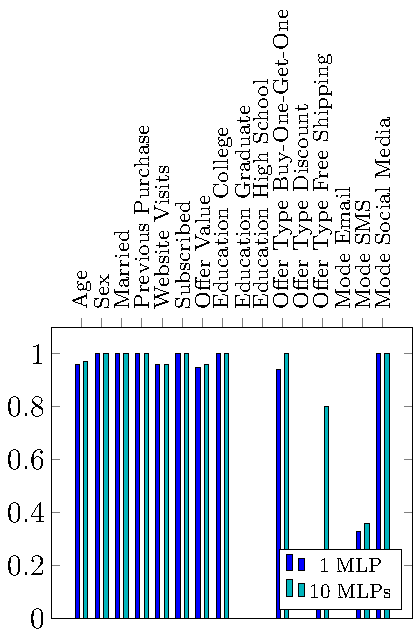
\includegraphics[width=.28\textwidth]{MarketingFigs/shap_mlp_avg-figure0.pdf}}%
                    \label{subfig:marketing_mlp_avg_shap_sign_accs}%
                }\hspace{1cm}
                \subfloat[SHAP Concordance]{%
                    \raisebox{.05cm}{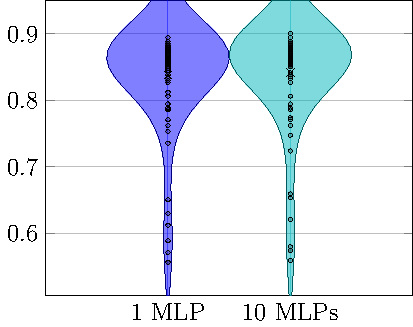
\includegraphics[width=.28\textwidth]{MarketingFigs/shap_mlp_avg-figure1.pdf}}%
                    \label{subfig:marketing_mlp_avg_shap_spearmans}%
                }\hspace{1cm}
                \subfloat[SHAP Relevance]{%
                    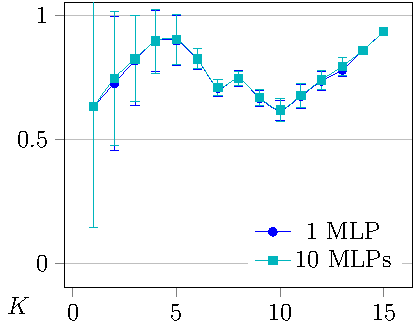
\includegraphics[width=.28\textwidth]{MarketingFigs/shap_mlp_avg-figure2.pdf}%
                    \label{subfig:marketing_mlp_avg_shap_recalls}%
                }\\
                \subfloat[LIME Directionality]{%
                    \raisebox{.2cm}{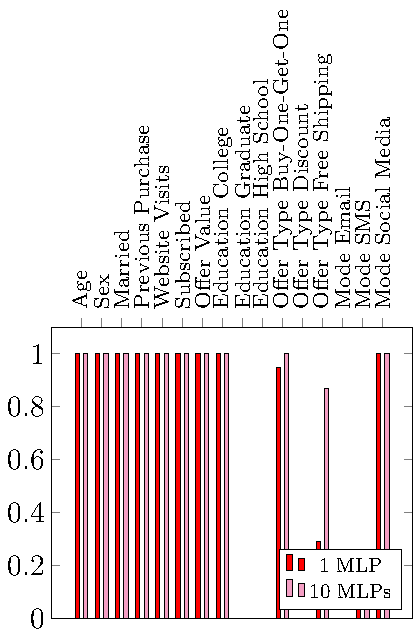
\includegraphics[width=.28\textwidth]{MarketingFigs/lime_mlp_avg-figure0.pdf}}%
                    \label{subfig:marketing_mlp_avg_lime_sign_accs}%
                }\hspace{1cm}
                \subfloat[LIME Concordance]{%
                    \raisebox{.05cm}{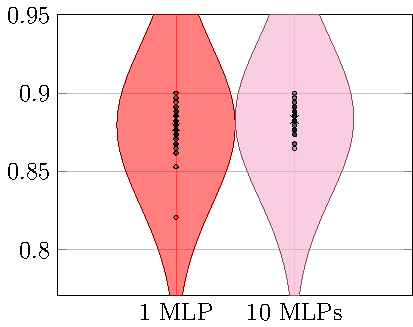
\includegraphics[width=.28\textwidth]{MarketingFigs/lime_mlp_avg-figure1.pdf}}%
                    \label{subfig:marketing_mlp_avg_lime_spearmans}%
                }\hspace{1cm}
                \subfloat[LIME Relevance]{%
                    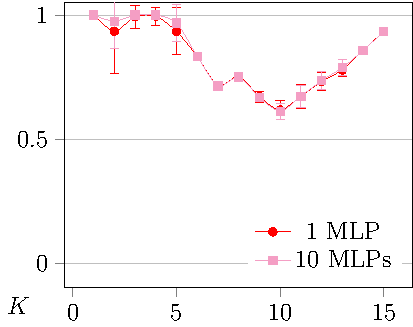
\includegraphics[width=.28\textwidth]{MarketingFigs/lime_mlp_avg-figure2.pdf}%
                    \label{subfig:marketing_mlp_avg_lime_recalls}%
                }\\
                \caption{Comparisons of results for our three metrics for SHAP (top row) and LIME (bottom row) explanations of 1 MLP versus explanations constructed by averaging the feature importance values of 10 MLPs.}
                \label{fig:marketing_mlp_increase}
            \end{figure}

        \subsubsection{Optimizing the Tradeoff between Complexity and Predictive Power}
            In this section we compare the data-alignment of explanations of models $\mathcal{M}_1$ with 100 neurons in its hidden layer and $\mathcal{M}_2$ with only 2 nodes in its hidden layer. Both models have a test set AUC of about .96. We found that the explanations of the simpler model $\mathcal{M}_2$ were more data-aligned with respect to relevance but less data-aligned with respect to concordance. Figure \ref{fig:marketing_decreasing_complexity} shows that the mean relevances for both SHAP and LIME were noticeably larger for $\mathcal{M}_2$ for many $k$ but the mean concordances for both SHAP and LIME were smaller for explanations of $\mathcal{M}_2$ than for explanations of $\mathcal{M}_1$.

            For SHAP, directionality was significantly improved for ``Mode: Email", ``Mode: SMS", and ``Offer Type: Free Shipping" with $p<.001$. Directionality for SHAP explanations of $\mathcal{M}_2$ was not significantly lower for any feature. Relevance was significantly improved for $k=1$ with $p\simeq .01$, $k=2$ with $p\simeq .04$, $k=5,\ldots,13$ with $p<.001$, and $k=14$ with $p\simeq .002$.  For LIME, directionality was also significantly improved for ``Mode: Email", ``Mode: SMS", and ``Offer Type: Free Shipping" with $p<.001$ and not significantly lower for any feature. Directionality was significantly improved for $k=6$ with $p\simeq .02$ and for $k=7,\ldots,14$ with $p<.001$. 

            
            \begin{figure}[t!]
                \subfloat[SHAP Directionality]{%
                    \raisebox{.2cm}{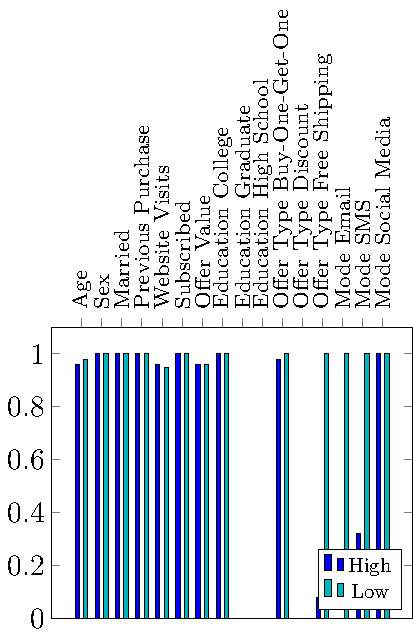
\includegraphics[width=.28\textwidth]{MarketingFigs/shap_cplx-figure0.pdf}}%
                    \label{subfig:marketing_decreasing_complexity_shap_sign_accs}%
                }\hspace{1cm}
                \subfloat[SHAP Concordance]{%
                    \raisebox{.05cm}{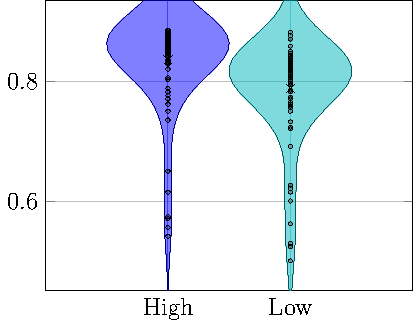
\includegraphics[width=.28\textwidth]{MarketingFigs/shap_cplx-figure1.pdf}}%
                    \label{subfig:marketing_decreasing_complexity_shap_spearmans}%
                }\hspace{1cm}
                \subfloat[SHAP Relevance]{%
                    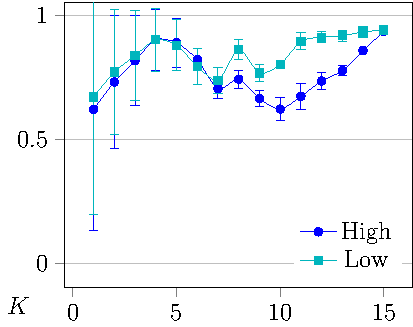
\includegraphics[width=.28\textwidth]{MarketingFigs/shap_cplx-figure2.pdf}%
                    \label{subfig:marketing_decreasing_complexity_shap_recalls}%
                }\\
                \subfloat[LIME Directionality]{%
                    \raisebox{.2cm}{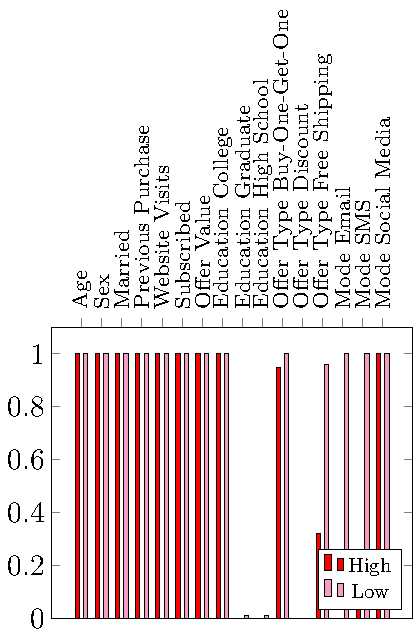
\includegraphics[width=.28\textwidth]{MarketingFigs/lime_cplx-figure0.pdf}}%
                    \label{subfig:marketing_decreasing_complexity_lime_sign_accs}%
                }\hspace{1cm}
                \subfloat[LIME Concordance]{%
                    \raisebox{.05cm}{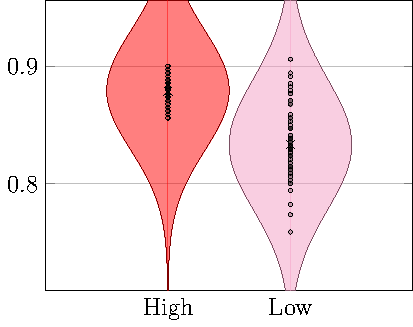
\includegraphics[width=.28\textwidth]{MarketingFigs/lime_cplx-figure1.pdf}}%
                    \label{subfig:marketing_decreasing_complexity_lime_spearmans}%
                }\hspace{1cm}
                \subfloat[LIME Relevance]{%
                    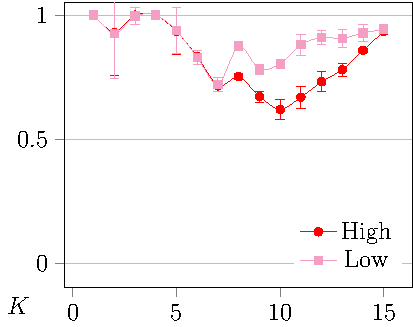
\includegraphics[width=.28\textwidth]{MarketingFigs/lime_cplx-figure2.pdf}%
                    \label{subfig:marketing_decreasing_complexity_lime_recalls}%
                }\\
                \caption{Comparisons of results for our three metrics for SHAP (top row) and LIME (bottom row) explanations of equally accurate MLPs with high and low complexity.}
                \label{fig:marketing_decreasing_complexity}
            \end{figure}


    



    
   
\end{document}
% %%%%%%%%%%%%%%%%%?